% /*@@
%   @file      UsersGuide.tex
%   @date      27 Jan 1999
%   @author    Tom Goodale, Gabrielle Allen, Gerd Lanferman
%   @desc 
%   Main file for the Cactus User's Guide
%   @enddesc 
%   @version $Header: /cactus/Cactus/doc/UsersGuide/UsersGuide.tex,v 1.32 2001/12/20 16:59:28 jthorn Exp $      
% @@*/

\documentclass{report}
\usepackage{fancyhdr,ifthen,calc}

\newif\ifpdf
\ifx\pdfoutput\undefined
\pdffalse % we are not running PDFLaTeX
\else
\pdfoutput=1 % we are running PDFLaTeX
\pdftrue
\fi

\ifpdf
\usepackage[pdftex]{graphicx}
\else
\usepackage{graphicx}
\fi


\makeatletter
\@addtoreset{chapter}{part}
\makeatother

%%%%%%%%%%%%%%%%%%%%%%%%%%%%%%%%%%%%%%%%%%%%%%%%%%%%%%%%%%%%%%%%%%%%%%%%%
\parskip = 0 pt
\parindent = 0pt
\oddsidemargin = 0 cm
\textwidth = 16 cm
\topmargin = -1 cm
\textheight = 24 cm

\usepackage{tocloft}
\addtolength{\cftchapnumwidth}{0.5em}
\addtolength{\cftsecnumwidth}{0.5em}
\addtolength{\cftsubsecnumwidth}{0.5em}
\addtolength{\cftsubsubsecnumwidth}{0.5em}

\def\q{\bf QUERY: }
\def\t{\tt \obeylines }
\def\ie{\hbox{i.e.\hbox{}}}

%%%%%%%%%%%%%%%%%%%%%%%%%%%%%%%%%%%%%%%%%%%%%%%%%%%%%%%%%%%%%%%%%%%%%%%%%%
\newenvironment{CCTKroutine}{\newpage}{}
\newenvironment{CCTKsyn}{\noindent\begin{tabular}{@{}p{3cm}cp{11cm}}&&\\{\bf Synopsis} \hfill&&\\}{\end{tabular}}
% The above needs to be fixed -- sometimes it runs off the page (e.g. with cctk_complex arguments...)
\newenvironment{CCTKpar}{\noindent\begin{tabular}{@{}p{3cm}cp{11cm}}&&\\{\bf Parameters} \hfill&&\\}{\end{tabular}}
\newcommand{\CCTKname}[1]{\noindent{\t #1}\hrule}
\newcommand{\CCTKdesc}[1]{\vskip .3cm \noindent #1}

%%%%%%%%%%%%%%%%%%%%%%%%%%%%%%%%%%%%%%%%%%%%%%%%%%%%%%%%%%%%%%%%%%%%%%%%
%Define some saveboxes to hold data
\newsavebox{\cctkbox}
\newsavebox{\cctkcargbox}
\newsavebox{\cctkfargbox}
\newsavebox{\cctkfargdefs}
\newsavebox{\cctkcsepbox}
\newsavebox{\cctkfsepbox}
\newsavebox{\cctkfdefssep}
\newsavebox{\cctkcprefix}
\newsavebox{\cctkfprefix}
\newsavebox{\cctkparambox}


%%%%%%%%%%%%%%%%%%%%%%%%%%%%%%%%%%%%%%%%%%%%%%%%%%%%%%%%%%%%%%%%%%%%%%%%%
% MANPAGE like description setting for options, use as 
% \begin{Lentry} \item[text] text  \end{Lentry}

\newcommand{\entrylabel}[1]{\mbox{\textsf{#1}}\hfil}
\newenvironment{entry}
  {\begin{list}{}
    {\renewcommand{\makelabel}{\entrylabel}
      \setlength{\labelwidth}{90pt}
      \setlength{\leftmargin}{\labelwidth+\labelsep}
    }
  }
  {\end{list}}

\newlength{\Mylen}
\newcommand{\Lentrylabel}[1]{%
  \settowidth{\Mylen}{\textsf{#1}}%
  \ifthenelse{\lengthtest{\Mylen > \labelwidth}}%
    {\parbox[b]{\labelwidth} %  term > labelwidth
      {\makebox[0pt][l]{\textsf{#1}}\\}} %
    {\textsf{#1}} %

  \hfil\relax}
\newenvironment{Lentry}
  {\renewcommand{\entrylabel}{\Lentrylabel}
   \begin{entry}}
  {\end{entry}}
%%%%%%

%%%%%%%%%%%%%%%%%%%%%%%%%%%%%%%%%%%%%%%%%%%%%%%%%%%%%%%%%%%%%%%%%%%%%%%%%%%

\newenvironment{CCTKFunc}[2]
        {\sbox{\cctkbox}{#1}
         \newpage
         \noindent{\t #1}\hrule 
         \vskip .3cm \noindent #2\\
%Clear the saveboxes - this may not be neccessary
         \sbox{\cctkcargbox}{}
         \sbox{\cctkfargbox}{}
         \sbox{\cctkfargdefs}{}
         \sbox{\cctkcsepbox}{}
         \sbox{\cctkfsepbox}{}
         \sbox{\cctkfdefssep}{}
         \sbox{\cctkcprefix}{}
         \sbox{\cctkfprefix}{}
%A command to add an argument - takes ctype, ftype, name
         \newcommand{\argument}[3]
         {\sbox{\cctkcargbox}{\usebox{\cctkcargbox}\usebox{\cctkcsepbox} ##1 ##3} 
          \sbox{\cctkcsepbox}{,}
          \sbox{\cctkfargbox}{\usebox{\cctkfargbox}\usebox{\cctkfsepbox} ##3} 
          \sbox{\cctkfsepbox}{,}
          \sbox{\cctkfargdefs}{\noindent{}\vbox{\noindent\usebox{\cctkfargdefs}\noindent\usebox{\cctkfdefssep}\noindent {}  ##2 ##3}}
          \sbox{\cctkfdefssep}{\\}
         }
%Use this command if it is a subroutine, same args as \argument
         \newcommand{\subroutine}[3]
         {\sbox{\cctkcprefix}{##1 ##3 =}
          \sbox{\cctkfprefix}{call}
          \sbox{\cctkfargbox}{##3\usebox{\cctkfsepbox} \usebox{\cctkfargbox}} 
          \sbox{\cctkfsepbox}{,}
          \sbox{\cctkfargdefs}{\noindent{}\vbox{\noindent ##2 ##3 \usebox{\cctkfdefssep}\noindent{}\usebox{\cctkfargdefs}}}
          \sbox{\cctkfdefssep}{\\}
         }

%Use this command if it is a function, same args as \argument
         \newcommand{\function}[3]
         {\sbox{\cctkcprefix}{##1 ##3 =}
          \sbox{\cctkfprefix}{##3 = }
          \sbox{\cctkfargdefs}{\noindent{}\vbox{\noindent ##2 ##3 \usebox{\cctkfdefssep}\noindent{}\usebox{\cctkfargdefs}}}
          \sbox{\cctkfdefssep}{\\}
         }

%Use this to display the arguments
         \newcommand{\showargs}
         {\noindent
          \begin{tabular}{@{}p{3cm}cp{11cm}}&&\\
{\bf Synopsis} \hfill&&\\ 
\hfill {\bf C} && {\t \usebox{\cctkcprefix} \usebox{\cctkbox}(\usebox{\cctkcargbox})}\\
\hfill {\bf Fortran} && 
{\t \usebox{\cctkfprefix} \usebox{\cctkbox}(\usebox{\cctkfargbox} ) }\\
&&\noindent\usebox{\cctkfargdefs}
\end{tabular}\\
}

%Use this to display the C arguments
         \newcommand{\showcargs}
         {\noindent
          \begin{tabular}{@{}p{3cm}cp{11cm}}&&\\
{\bf Synopsis} \hfill&&\\ 
\hfill {\bf C} && {\t \usebox{\cctkcprefix} \usebox{\cctkbox}(\usebox{\cctkcargbox})}\\
\end{tabular}\\
}


%Environment for describing parameters
          \newenvironment{params}{
             \noindent\begin{tabular}{@{}p{3cm}cp{11cm}}&&\\{\bf Parameters} \hfill&&\\}{\end{tabular}\\}
%Command to describe a parameter, takes name and description
          \newcommand{\parameter}[2]{
\\
\hfill {\t ##1} &-&##2
\\
}
%Environment for discussion
    \newenvironment{discussion}
    {\noindent
     \begin{tabular}{@{}p{14cm}}
     \\{\bf Discussion} \hfill\\
    }
    {
     \end{tabular}\\
    }
%Environment for examples
    \newenvironment{examples}
    {\noindent
     \begin{tabular}{@{}p{14cm}}
     \\{\bf Examples} \hfill\\
    }
    {
     \end{tabular}\\\\
    }

%Environment for describing errors
     \newenvironment{errorcodes}
    {\noindent
     \begin{tabular}{@{}p{6cm}cp{10cm}}&&\\
     {\bf Errors} \hfill&&\\}
    {\end{tabular}\\}
%Command to describe an errorcode, takes name and description
          \newcommand{\errorcode}[2]{
\\
\hfill {\t ##1} &-&##2
\\
}

}% end of \begin{CCTKFunc} expansion
{}% \end{CCTKFunc} expansion

%%%%%%%%%%%%%%%%%%%%%%%%%%%%%%%%%%%%%%%%%%%%%%%%%%%%%%%%%%%%%%%%%%%%%%%%%%%

%
% Alternate environments/macros to define function descriptions
% (can/should be used to replace CCTKFunc environment)
% Jonathan Thornburg, 10 Nov 2001
%
% Usage:
%	\begin{FunctionDescription}{name}
%	\label{label}
%	Synopsis for this function			(running text rules)
%
%	\begin{Synopsis}{C}
%	text of C function synopsis			(running text rules)
%	\end{Synopsis}
%	\begin{Synopsis}{Fortran}
%	text of Fortran function synopsis		(running text rules)
%	\end{Synopsis}
%
%	\begin{ResultNote}
%	note to go at the beginning of all results	(running text rules
%	(this is optional; omit the ResultNote environment if not needed)
%	\end{ResultNote}
%	\begin{Result}{name or value (automatically in \tt font)}
%	desription of what the result means in general,
%	or of what this particular result value means	(running text rules)
%	\end{Result}
%
%	\begin{Parameter}{name (automatically in \tt font)}
%	desription of parameter				(running text rules)
%	\end{Parameter}
%	\begin{Parameter}{name2 (automatically in \tt font)}
%	desription of another parameter			(running text rules)
%	\end{Parameter}
%	\begin{Discussion}
%	discussion					(running text rules)
%	\NewPar
%	another paragraph of discussion			(running text rules)
%	\NewPar
%	yet another paragraph of discussion		(running text rules)
%	\end{Discussion}
%
%	\begin{SeeAlso}{name (automatically in \tt font)
%	cross-references to other function of that name (running text rules)
%	\end{SeeAlso}
%	\begin{SeeAlso}{name2 (automatically in \tt font)
%	cross-references to another function            (running text rules)
%	\end{SeeAlso}
%
%	\begin{Error}{error\_code (automatically in \tt font)}
%	description of what this error code means	(running text rules)
%	\end{Error}
%	\begin{Error}{error\_code2 (automatically in \tt font)}
%	description of what next error code means	(running text rules)
%	\end{Error}
%
%	\begin{Example}{C}
%	example C code					(running text rules)
%	\end{Example}
%	\begin{Example}{Fortran}
%	example Fortran code				(running text rules)
%	\end{Example}
%
% For arguments which are automatically in \tt font, \rm may be used
% to switch back to normal Roman font (eg for a numerical value), and
% $...$ may be used for math mode (eg  ($\ge 0$)  to mark a result
% which is always non-negative).
%
% Each "running text rules" item is the body of a latex environment,
% so it may include multiple lines or even paragraphs.  Normally
% underscore must be escaped (\_), but  \verb|...|  and/or
%	\begin{verbatim}
%	...
%	\end{verbatim}
% or similar constructs (which can't be used inside a macro argument)
% may also be used (in which case _ { } \ etc need not be escaped).
%
% Within a multi-paragraph "running text rules" item, \NewPar should be
% used at the start of each new paragraph.
%
% All the subsections are optional.
%
% Bugs:
% - There are various hardcoded lengths which should ideally be global
%   style parameters, and/or be determined from other style parameters
%   and \textwidth
% - It would be nice if we could avoid having to escape underscore
%   within arguments.
% - Error checking: if you have to ask, there isn't enough for you! :)
% - The vertical spacing is a bit of a hack.  Notably, having to use
%   \NewPar is an awful kludge -- \par should be redefined to do this
%   automagically.
% - There are no controls to prevent a page break falling between the
%   line "C" or "Fortran", and an immediately following example generated
%   by the Example subenvironment.  In fact, LaTeX seems to like doing
%   this. :(
% - It would be nice to have a "...continued" legend at the bottom of
%   all but the last page of a multi-page description.
% - The running header giving the function name, only appears for the
%   first page of a multi-page description.
% - In some ideal world, "See Also" would generate pdf hotlinks.
% - Footnotes don't work properly -- they come out at the bottom of
%   the individual section, not at the bottom of the page.
%   
\newenvironment{FunctionDescription}[1]
{
\def\NewPar{\vskip0.5\baselineskip}
\newpage
\noindent{\t #1}
\vskip1mm
\hrule 
\vskip3mm
%
% We define all the subenvironments inside the main one, so they won't
% interfere with any conflicting global definitions.
%
% We want to generate a heading for the *first* Synopsis, Result, Parameter,
% SeeAlso, Error, or Example environment, but not for later ones, so for
% each of these environments we first \gdef the desired heading, then have
% the environment redefine it to be empty (or just some vspace).
%
\gdef\SynopsisHeading{{\bf Synopsis}\\}%%%
\newenvironment{Synopsis}[1]
               {%%%
               \par
               \noindent\SynopsisHeading
               \gdef\SynopsisHeading{{\bf \ }\\[-0.5\baselineskip]}%%%
               \hbox to 25mm{\hfill\bf ##1}\quad\begin{minipage}[t]{125mm}
               }
               {%%%
               \end{minipage}
               \hrule height0ex depth0ex	% advance vertically down to
				               % end of above minipage box
               }
\gdef\ResultHeading{{\bf Result}\\}%%%
\newenvironment{ResultNote}
               {%%%
               \par
               \noindent\ResultHeading
               \gdef\ResultHeading{{\bf \ }\\[-0.5\baselineskip]}%%%
               \begin{minipage}[t]{150mm}
               }
               {%%%
               \end{minipage}
               \hrule height0ex depth0ex	% advance vertically down to
						% end of above minipage box
               }
\newenvironment{Result}[1]
               {%%%
               \par
               \noindent\ResultHeading
               \gdef\ResultHeading{{\bf \ }\\[-0.5\baselineskip]}%%%
               \hbox to 25mm{\hfill\t ##1}\quad\begin{minipage}[t]{125mm}
               }
               {%%%
               \end{minipage}
               \hrule height0ex depth0ex	% advance vertically down to
						% end of above minipage box
               }
\gdef\ParameterHeading{{\bf Parameters}\\}%%%
\newenvironment{Parameter}[1]
               {%%%
               \par
               \noindent\ParameterHeading
               \gdef\ParameterHeading{{\bf \ }\\[-0.5\baselineskip]}%%%
               \hbox to 25mm{\hfill\t ##1}\quad\begin{minipage}[t]{125mm}
               }
               {%%%
               \end{minipage}
               \hrule height0ex depth0ex	% advance vertically down to
						% end of above minipage box
               }
\newenvironment{Discussion}
               {%%%
               \par
               \noindent{\bf Discussion}\\
               \hbox to 25mm{\hfill}\quad\begin{minipage}[t]{125mm}
               }
               {%%%
               \end{minipage}
               \hrule height0ex depth0ex	% advance vertically down to
						% end of above minipage box
               }
\gdef\SeeAlsoHeading{{\bf See Also}\\}%%%
\newenvironment{SeeAlso}[1]
               {%%%
               \par
               \noindent\SeeAlsoHeading
               \gdef\SeeAlsoHeading{{\bf \ }\\[-0.5\baselineskip]}%%%
               \hbox to 55mm{\hfill\t ##1}\quad\begin{minipage}[t]{95mm}
               }
               {%%%
               \end{minipage}
               \hrule height0ex depth0ex	% advance vertically down to
						% end of above minipage box
               }
\gdef\ErrorHeading{{\bf Errors}\\}%%%
\newenvironment{Error}[1]
               {%%%
               \par
               \ErrorHeading
               \gdef\ErrorHeading{{\bf \ }\\[-0.5\baselineskip]}%%%
               \hbox to 55mm{\hfill\t ##1}\quad\begin{minipage}[t]{95mm}
               }
               {%%%
               \end{minipage}
               \hrule height0ex depth0ex	% advance vertically down to
						% end of above minipage box
               }
\gdef\ExampleHeading{{\bf Examples}\\}%%%
\newenvironment{Example}[1]
               {%%%
               \par
               \ExampleHeading
               \gdef\ExampleHeading{{\bf \ }\\[-0.5\baselineskip]}%%%
               \hbox to 25mm{\hfill\bf ##1}\\	% put #1 on a line by itself
               \hbox to 25mm{\hfill}\quad\begin{minipage}[t]{125mm}
               }
               {%%%
               \end{minipage}
               \hrule height0ex depth0ex	% advance vertically down to
						% end of above minipage box
               }
}% end of \begin{FunctionDescription} expansion
{}% \end{FunctionDescription} expansion is empty

%%%%%%%%%%%%%%%%%%%%%%%%%%%%%%%%%%%%%%%%%%%%%%%%%%%%%%%%%%%%%%%%%%%%%%
% Takes three arguments - the name of the document, the revision, and
% the date.
% Additionally ther eis an optional first argument with the version number

\newcommand{\cactustitlepage}[4][4.0]
{
\thispagestyle{empty}
\setlength{\parindent}{0mm}
\setlength{\parskip}{0mm}
\vspace*{\stretch{1}}
\rule{\linewidth}{1mm}
\begin{flushright}
  \Huge Cactus #1\\[5mm]
        #2
\end{flushright}
\rule{\linewidth}{1mm}
\vspace*{\stretch{2}}
\begin{center}
\ifpdf
\else

\includegraphics[angle=0,width=5cm]{bincactus2.eps}
\fi
\end{center}
\vspace*{\stretch{2}}
\begin{center}
   \Large #3 \\[3mm]
          #4
\end{center}
\newpage
\setlength{\parindent}{0mm}
\setlength{\parskip}{0mm}
}
%%%%%%%%%%%%%%%%%%%%%%%%%%%%%%%%%%%%%%%%%%%%%%%%%%%%%%%%%%%%%%%%%%%%%%%%%%%%%

\newenvironment{cactuspart}[4]
{
  \clearpage
  \renewcommand{\thepage}{\Alph{part}\arabic{page}}
  % Redefine the plain style
  \fancypagestyle{plain}
  {
    \fancyhf{} % Clear all header and footer fields
    \lfoot{#3}
    \cfoot{#4}
    \rfoot{\thepage/\pageref{lastpage:\thepart}}
    \renewcommand{\headrulewidth}{0.0pt}  
    \renewcommand{\footrulewidth}{0.4pt}  
    \renewcommand{\thepage}{\Alph{part}\arabic{page}}
  }

  % Make sure it's arabic numbering
  \pagenumbering{arabic}
  % Start the page counter at 1
  \setcounter{page}{1}
  % Start a new part
  \renewcommand{\thepage}{\Alph{part}\arabic{page}}
  \part{#2}
  \setcounter{part}{#1}
  % Redefine the page
  % Set up fancy headings.
  \lfoot{#3}
  \cfoot{#4}
  \rfoot{\thepage/\pageref{lastpage:\thepart}}
  \renewcommand{\headrulewidth}{0.4pt}
  \renewcommand{\footrulewidth}{0.4pt}
}
{
  % Remember the last page of the 
  \label{lastpage:\thepart}
  \clearpage
}


%%%%%%%%%%%%%%%%%%%%%%%%%%%%%%%%%%%%%%%%%%%%%%%%%%%%%%%%%%%%%%%%%%%%%%%%%%%%%
%%%%%%%%%%%%%%%%%%%%%%%%%%%%%%%%%%%%%%%%%%%%%%%%%%%%%%%%%%%%%%%%%%%%%%%%%%%%%

\begin{document}

\ifpdf
\DeclareGraphicsExtensions{.pdf, .jpg}
\else
\DeclareGraphicsExtensions{.eps, .jpg}
\fi

\cactustitlepage{Users' Guide}{$$Revision: 1.32 $$}{$$Date: 2001/12/20 16:59:28 $$}

\setcounter{page}{1}

% Table of contents
\pagenumbering{roman}

\tableofcontents

%%%%%%%%%%%%%%%%%%%%%%%%%%%%%%%%%%%%%%%%%%%%%%%%%%%%%%%%%%%%%%%%%%%%%%%
%%%%%%%%%%%%%%%%%%%%%%%%%%%%%%%%%%%%%%%%%%%%%%%%%%%%%%%%%%%%%%%%%%%%%%%
%%%%%%%%%%%%%%%%%%%%%%%%%%%%%%%%%%%%%%%%%%%%%%%%%%%%%%%%%%%%%%%%%%%%%%%

\renewcommand{\thepart}{\Alph{part}}
\renewcommand{\thechapter}{\Alph{part}\arabic{chapter}}
\renewcommand{\thepage}{\Alph{part}\arabic{page}}
\pagestyle{fancy}
\parskip = 10 pt
\parindent = 0pt

\newpage

%%%%%%%%%%%%%%%%%%%%%%%%%%%%%%%%%%%%%%%%%%%%%%%%%%%%%%%%%%%%%%%%%%%%%%%
%%%%%%%%%%%%%%%%%%%%%%%%%%%%%%%%%%%%%%%%%%%%%%%%%%%%%%%%%%%%%%%%%%%%%%%
%%%%%%%%%%%%%%%%%%%%%%%%%%%%%%%%%%%%%%%%%%%%%%%%%%%%%%%%%%%%%%%%%%%%%%%

% /*@@
%   @file      Preface.tex
%   @date      27 Jan 1999
%   @author    Tom Goodale, Gabrielle Allen, Gerd Lanferman
%   @desc 
%   Preface for the Cactus User's Guide
%   @enddesc 
%   @version $Header: /cactus/Cactus/doc/UsersGuide/Preface.tex,v 1.7 2001/12/17 10:06:13 rideout Exp $      
% @@*/

%%%%%%%%%%%%%%%%%%%%%%%%%%%%%%%%%%%%%%%%%%%%%%%%%%%%%%%%%%%%%%%%%%%%%%%
%%%%%%%%%%%%%%%%%%%%%%%%%%%%%%%%%%%%%%%%%%%%%%%%%%%%%%%%%%%%%%%%%%%%%%%

{\large \bf Preface} 
\label{sec:pr}
 
\vskip .5cm

This document will eventually be a complete guide to using and
developing with the Cactus Code. However, it is currently under
development, so please be patient if you can't find what you need.
Please report omissions, errors, or suggestions to 
and of our contact addresses below, and we will
try and fix them as soon as possible. 

\vskip .5cm

{\bf Overview of documentation}

\vskip .5cm

This guide covers the following topics

\begin{Lentry}

\item [{\bf Part A: Installation and Running.}]
  We give an overview of required hardware and
  software and talk you through the installation of a working
  Cactus tool kit. 
  You will be able to verify the correct installation with our
  test suite technology. 

\item [{\bf Part B: Application Thorn Writing.}] We introduce thorn
  concepts and describe all you need to know for creating, writing
  and maintaining application thorns. You will learn how to use the
  programming interface to take advantage of parallelism and modularity.

\item [{\bf Part C: Infrastructure Thorn Writer's Guide.}] In this more
  advanced part, we talk about user supplied infrastructure routines such
  as {\em additional output routines, drivers, etc.} [This part is not
  yet complete, and is currently under construction.]

\item [{\bf Part D: Function Reference.}] Here all Cactus flesh functions which
are available to thorn writers in C and Fortran are described.

\item [\bf Part E: Appendices.] These contain a description of the
Cactus Configuration Language, and other odds and ends, such as how to
use GNATS or TAGS.

\end{Lentry}

Other topics to be discussed in separate documents include:

\begin{Lentry}

\item [{\bf Computational Thorn Guide}] This will contain details about the 
arrangements and thorns making up the standard Cactus Computational Tool Kit.

\item [{\bf Relativity Thorn Guide}] This will contain details about the arrangements and thorns making up the Cactus Relativity Tool Kit, one of the major 
 motivators, and still the driving force, for the Cactus Code.

\item [{\bf Flesh Maintainers Guide}] 
 This will contain all the gruesome details
 about the inner workings of Cactus, for all those who want or need to 
 expand or maintain the core of Cactus.

\end{Lentry}

\vskip .5cm

{\bf Typographical Conventions}

\begin{Lentry}

\item[{\tt Typewriter}] Is currently used for everything you type,
	for program names, and code extracts.
\item[{\tt < ... >}] Indicates a compulsory argument.
\item[{\tt [ ... ]}] Indicates an optional argument.

\end{Lentry}
 
\vskip .5cm

{\bf How to Contact Us}

\vskip .5cm

Please let us know of any errors or omissions in this guide, as well
as suggestions for future editions. These can be reported via our 
bug tracking system at {\tt www.cactuscode.org}, or via email to
{\tt cactus@cactuscode.org}. Alternatively, write to us at

\vskip .5cm
The Cactus Team\\
Albert Einstein Institute\\
Max Planck Institute for Gravitational Physics\\
Am M\"{u}hlenberg 1\\
D-14476 Golm\\
Germany


\vskip .5cm

{\bf Acknowledgements}

\vskip .5cm

Hearty thanks to all those who have helped with documentation for the
Cactus Code. Special thanks to those who struggled with the earliest
sparse versions of this guide and sent in mistakes and suggestions,
in particular John Baker, Carsten Gundlach, Ginny Hudak-David, 
Sai Iyer, Paul Lamping, Nancy Tran and Ed Seidel. 



% /*@@
%   @file      RunningCactus.tex
%   @date      27 Jan 1999
%   @author    Tom Goodale, Gabrielle Allen, Gerd Lanferman
%   @desc 
%   How to run Cactus part of the Cactus User's Guide
%   @enddesc %   @version $Header: /cactus/Cactus/doc/UsersGuide/RunningCactus.tex,v 1.75 2002/01/02 16:32:04 tradke Exp $      
% @@*/
\begin{cactuspart}{1}{Installation and Running}{$RCSfile: RunningCactus.tex,v $}{$Revision: 1.75 $}
\renewcommand{\thepage}{\Alph{part}\arabic{page}}



%%%%%%%%%%%%%%%%%%%%%%%%%%%%%%%%%%%%%%%%%%%%%%%%%%%%%%%%%%%%%%%%%%%%%%%
%%%%%%%%%%%%%%%%%%%%%%%%%%%%%%%%%%%%%%%%%%%%%%%%%%%%%%%%%%%%%%%%%%%%%%%

\chapter{Installation} 
\label{cha:in}

%%%%%%%%%%%%%%%%%%%%%%%%%%%%%%%%%%%%%%%%%%%%%%%%%%%%%%%%%%%%%%%%%%%%%%%

\section{Required software}
\label{sec:reqo}

In general, Cactus {\em requires} the following set of software to function
in single processor mode. Please refer to the architecture section
\ref{sec:suar} for architecture specific items.
\begin{Lentry}
\item[{\tt Perl5.0}] Perl is used extensively during the Cactus
  thorn configuration phase. Perl is available for nearly all
  operating systems known to man and can be obtained at
  {\tt http://www.perl.org}
\item[{\tt GNU make}] The make
  process works with the GNU make utility (referred to as {\bf gmake} 
  henceforth). While other make utilities may also work, this is not 
  guaranteed. Gmake can be obtained from your favorite GNU site or
  from {\tt www.gnu.org}
\item[{\tt C}] C compiler. For example, the GNU compiler. This
 is available for most supported platforms.  Platform specific compilers 
 should also work. 
\item[{\tt CPP}] C Pre-processor. For example, the GNU CPP.  These are
normally provided on most platforms, and many C compilers have an option
to just run as a preprocessor.
\item[{\tt CVS}] The {\em ``Concurrent Versioning System''} is not needed
  to run/compile Cactus, but you are strongly encourage to install
  this software to take advantage of the update procedures. It can be
  downloaded from your favorite GNU site.  Tar files of each release are
  also available.
\end{Lentry}

\noindent
To use Cactus, with the default driver\footnote{For help with unfamiliar terms, please consult the glossary, Appendix \ref{sec:glossary}.} ({\tt CactusPUGH/PUGH}) on multiple
processors you also need:
\begin{Lentry}
\item[{\tt MPI}] the {\it Message Passing Interface (MPI)} 
which provides inter-processor communication. 
Supercomputing sites often supply a native {\tt MPI} implementation with
which Cactus is very likely to be compatible. Otherwise there are
various freely available ones available, e.g. the {\tt MPICH}
version of {\tt MPI} is available for various architectures and operating
systems at {\tt http://www-unix.mcs.anl.gov/mpi/}. 
\end{Lentry}

\noindent
If you are using any thorns containing routines 
written in {\tt C++} you also need
\begin{Lentry}
\item[{\tt C++}] C++ compiler. For example, the GNU compiler. This
 is available for most supported platforms.  Platform specific compilers 
 should also work.  Note that if a C++ compiler is available then the
 {\em main} routine in the flesh is compiled with C++ to allow static
 class initialisations.
\end{Lentry}

\noindent
If you are using any thorns containing routines 
written in {\tt FORTRAN} you also need
\begin{Lentry}
\item[{\tt F90/F77}] For routines written in F77, either an F90 or an F77
 compiler can be used. For routines written in F90 a F90 compiler is
 obviously
 required. There is a very limited set of free F90 compilers available
 for the different architectures.
\end{Lentry}

\noindent
While not required for compiling or running Cactus, for thorn development
it is useful to install
\begin{Lentry}
\item[{\tt ctags/etags}] The program Tags enables you browse through the calling structure
  of a program by help of a function call database. Navigating the flesh and
  arrangements becomes very easy. Emacs and vi both support this method. See
  \ref{sec:usta} for a short guide to ``tags''.
\end{Lentry}

%%%%%%%%%%%%%%%%%%%%%%%%%%%%%%%%%%%%%%%%%%%%%%%%%%%%%%%%%%%%%%%%%%%%%%%

\section{Supported architectures}
\label{sec:suar}

Cactus runs on many machines, under a large number of operating
systems.  Here we list the machines we have compiled and verified
Cactus on, including some architecture specific notes.  A complete
list of architectures supported by Cactus, along with more notes, can
be found at
\begin{center}
{\tt http://www.cactuscode.org/Documentation/Architectures.html}.
\end{center}

\begin{Lentry} 
\item[{\bf SGI}] 32 or 64 bit running Irix.
\item[{\bf Cray T3E}]
\item[{\bf Compaq Alpha}]  Compaq operating system and Linux.  Single processor
  mode and {\tt MPI} supported. The Alphas need to have the GNU {\tt C/C++}
  compilers installed.
\item[\textbf{IA32}] running Linux or Windows 2000/NT.  Single
processor mode and MPI ({\tt MPICH} and {\tt LAM}) supported.\\On
Windows Cactus compiles with Cygwin.  MPI
({\tt WMPI}, {\tt HPVM}, and {\tt MPIPro}) supported.  Please read
doc/README.NT for details.
\item[\textbf{IA64}]  running Linux.
\item[{\bf Macintosh PowerPC}] (MacOS X and Linux PPC)
\item[{\bf IBM SP2}]
\item[{\bf Hitachi SR8000-F1}]
\item[{\bf Sun} Solaris]
\item[{\bf Fujitsu}]
\end{Lentry}

%\begin{Lentry} 
%\item[{\bf SGI Origin 2000} running Irix]
%\item[{\bf SGI} 32 or 64 bit running Irix]
%\item[{\bf Cray T3E}] 
%\item[{\bf Dec Alpha}]  Dec operating system and Linux. Single processor
%  mode and {\tt MPI} supported. The Decs need to have the GNU {\tt C/C++} 
%  compilers installed 
%\item[{\bf Linux (ia32, ia64, ppc, alpha)}] There is a
%  free Linux F90 compiler available from  {\tt http://www.psrv.com}
%  -- the only free we know of; please note the comment about installing this in 
%the FAQ.
%  Single processor mode and MPI ({\tt MPICH} and {\tt LAM}) supported.
%\item[{\bf Windows NT}] Compiles with Cygwin. Single processor mode and MPI ({\t
%t WMPI}, 
%{\tt HPVM}, and {\tt MPIPro}) supported.  Please read doc/README.NT for details.
%\item[{\bf Macintosh PowerPC (MacOS X)}]
%\item[{\bf IBM SP2}]
%\item[{\bf Hitachi SR8000-F1}]
%\item[{\bf Sun Solaris}]  
%\end{Lentry}

The following machines are only partially supported
\begin{Lentry}
\item[{\bf HP Exemplar}] 
\item[{\bf NEC SX-5}]
\end{Lentry}

%%%%%%%%%%%%%%%%%%%%%%%%%%%%%%%%%%%%%%%%%%%%%%%%%%%%%%%%%%%%%%%%%%%%%%%

\section{Checkout procedure}
\label{sec:chpr}

Cactus is distributed, extended, and maintained using the free CVS
software ({\it Concurrent Versioning System}: {\tt http://www.cvshome.org}). 
CVS  allows many people to work on a large software project 
together without getting into a tangle. 
Since Cactus thorns are distributed from several repositories on the
main CVS site, and from a growing number of user sites, we provide a
script, described below,  on our website for checking out the flesh and thorns.
The Cactus website also provides a form interface for direct download.

CVS experts who want to use raw CVS commands are directed to Appendix~\ref{sec:uscv}
for full instructions. For CVS novices, we also summarize in this
appendix basic CVS commands.

The space required for an installation depends on the arrangements and
thorns used. The flesh on its own requires less than 5 MB.

The script for checking out the flesh and thorns, {\tt GetCactus}, is available 
from the website at 

{\tt http://www.cactuscode.org/Download/GetCactus}

The 
script takes as an argument the name of a file containing a {\it ThornList},
that is a list of thorns with the syntax 
{\tt
\begin{verbatim}
<arrangement name>/<thorn name>
\end{verbatim}
}
If no filename is given, only the flesh is checked out.
Optional directives in the ThornList indicate which CVS repository to fetch 
thorns from. The default is to take the thorns from the same repository as
the flesh. A full description of ThornList syntax is provided in Appendix~\ref{chap:th}.
ThornLists for example applications are provided on the Cactus website.

The same script can be used to checkout additional thorns.

%%%%%%%%%%%%%%%%%%%%%%%%%%%%%%%%%%%%%%%%%%%%%%%%%%%%%%%%%%%%%%%%%%%%%%%

\section{Directory structure}
\label{sec:dist}

A fresh checkout creates a directory {\tt Cactus} with the
following subdirectories:

\begin{Lentry}

\item[{\tt CVS}] the CVS book-keeping directory, present in every subdirectory

\item[{\tt doc}] Cactus documentation

\item[{\tt lib}] contains libraries

\item[{\tt src}] contains the source code for Cactus

\item [{\tt arrangements}] contains the Cactus arrangements. The arrangements
  (the actual ``physics'') are not supplied by checking out just Cactus. 
  If the arrangements you want to use are standard Cactus arrangements, or
  reside on our CVS repository ({\tt cvs.cactuscode.org}), 
  they can be checked out in similar way to the Flesh. 
\end{Lentry}

When Cactus is first compiled it creates a new directory {\tt
Cactus/configs}, which will contain all the source code, object files and
libraries created during the build process.  Disk space may be a problem 
on supercomputers where home directories are small. 

A workaround is to first create a
configs directory on scratch space, say {\tt scratch/cactus\_configs/} (where
{\tt scratch/} is your scratch directory), and then either
\begin{itemize}
\item{} set the environment variable {\tt CACTUS\_CONFIGS\_DIR} to point to 
this directory
\end{itemize}
or
\begin{itemize}
\item{}  soft link this directory ({\tt ln -s
scratch/cactus\_configs Cactus/configs/}) to the Cactus directory, if your
file-system supports soft-links.
\end{itemize}

Configurations are described in detail in section \ref{sec:coaco}.

%%%%%%%%%%%%%%%%%%%%%%%%%%%%%%%%%%%%%%%%%%%%%%%%%%%%%%%%%%%%%%%%%%%%%%%

\section{Getting help}
\label{sec:gehe}

For tracking problem reports and bugs we use GNATS, which is a bugtracking 
system published under the GNU license. We have set up a web interface at 
{\tt http://www.cactuscode.org} which allows easy submission and browsing 
of problem reports.    

A description of the GNATS categories which we use is provided in the appendix 
\ref{sec:usgn}.

% OK, there is NO emacs at the moment, because the GNATS setup is really stupid
% and sendpr handles like c.... besides the fact, that the user has to go 
% through a make-process which installs stuff somewhere on his HD. gerd.
% BUT, we could distribute our own, either copy cvsbug, or write a perl
% version.  Tom
% \begin{itemize}
% \item {\tt A web interface}
% \item {\tt SendPR}
% {FIXME: Mention the emacs thing here too...}
% \end{itemize}

%%%%%%%%%%%%%%%%%%%%%%%%%%%%%%%%%%%%%%%%%%%%%%%%%%%%%%%%%%%%%%%%%%%%%%%
%%%%%%%%%%%%%%%%%%%%%%%%%%%%%%%%%%%%%%%%%%%%%%%%%%%%%%%%%%%%%%%%%%%%%%%

\chapter{Compilation} 

%%%%%%%%%%%%%%%%%%%%%%%%%%%%%%%%%%%%%%%%%%%%%%%%%%%%%%%%%%%%%%%%%%%%%%%


Cactus can be built in different configurations from the same copy of
the source files, and these different configurations coexist in the
{\tt Cactus/configs} directory. Here are several instances in which
 this can be useful:

\begin{enumerate}
\item{}Different configurations can be for {\em different
architectures}. You can keep executables for multiple architectures
based on a single copy of source code, shared on a common file
system.
\item{} You can compare different {\em compiler options, debug-modes}.
  You might want to compile different communication protocols
  (e.g. {\tt MPI} or {\tt GLOBUS}) or leave them out all together.
\item{} You can have different configurations for {\em different thorn
    collections} compiled into your executable.
\end{enumerate}

Once a configuration has been created, by {\tt gmake <config>} as described
in detail in the next section, a single call to {\tt gmake <config>}
will compile the code.  The first time it generates a compile 
{\tt ThornList},  and gives you the chance to edit it before continuing.

%%%%%%%%%%%%%%%%%%%%%%%%%%%%%%%%%%%%%%%%%%%%%%%%%%%%%%%%%%%%%%%%%%%%%%%
\section{Creating a configuration}
\label{sec:coaco}

At its simplest, this is done by {\tt gmake <config>}.  This generates
a configuration with the name {\tt config}, doing its best to automatically
determine the default compilers and compilation flags suitable for the current 
architecture.

There are a number of additional command line arguments which may be supplied 
to override some parts of the procedure.

\subsection{Configuration options}

There are three ways to pass options to the configuration process.
% from the gmake command line.  
\begin{enumerate}
\item{} Create a file \texttt{\~{ }/.cactus/config}.

All available configuration options may be set in the file {\tt
\~{ }/.cactus/config}, any which are not set will take a default value.
The file should contain lines of the form:

{\tt <option> [=] ...}

The equals sign is optional.

\item{} Add the options to a configuration file and use,\\
{\tt gmake <config>-config  options=<filename>}
The options file has the same format as {\tt \~/.cactus/config}.

\item{} Pass the options individually on the command line,\\
{\tt gmake <configuration name>-config  <option name>=<chosen value>, ...}
Not all configuration options can be set on the command line.  Those that can
be set are indicated in the table below.
\end{enumerate}

They are listed here in order of increasing precedence, e.g. options
set on the command line will take priority over (potentially
conflicting) options set in \texttt{\~{ }/.cactus/config}.
%Note that if a configuration file is used, and options are also passed
%on the command line, the command line options will override those from
%the configuration file.

It is important to note that these methods cannot be used to, for example add
options to the default values for {\tt CFLAGS}.  Setting {\tt CFLAGS} in the
configuration file or the command line will overwrite completely the 
default values.

\subsection{Available options}
\label{Compilation-Available_Options}

There is a plethora of available options.

\begin{itemize}

\item {\tt Compiled Thorns}

These specify the chosen set of thorns for compilation. If the thorn choice is not provided
during configuration, a list containing all thorns in the {\tt arrangements} directory
is automatically created, and the users prompted for any changes.

\begin{Lentry}

\item [{\tt THORNLIST}] Name of file containing a list of thorns with
the syntax {\tt <arrangement name>/<thorn name>}, lines beginning with
\# or ! are ignored.

\item [{\tt THORNLIST\_DIR}] Location of directory containing {\tt THORNLIST}.

%\item [{\tt THORNS}] List of thorns to use for compilation. This option can be used in 
% 	conjunction with {\tt THORNLIST}. NOTE: In Beta 10 this will change to {\tt THORNLIST}.

\end{Lentry}

\item {\tt Compiler and tool specification}

These are used to specify which compilers and other tools to use. Entries followed
by * may be specified on the command line.

\begin{Lentry}
\item [{\tt CC}]
* The C compiler.
\item [{\tt CXX}]
The C++ compiler.
\item [{\tt F90}]
* The Fortran 90 compiler.
\item [{\tt F77}]
* The FORTRAN 77 compiler.
\item [{\tt CPP}]
  The preprocessor used to generate dependencies and to preprocess Fortran code.
\item [{\tt LD}]
* The linker.
\item [{\tt AR}]
The archiver used for generating libraries.
\item [{\tt RANLIB}]
The archive indexer to use.
\item [{\tt MKDIR}]
The program to use to create a directory.
\item [{\tt PERL}]
The name of the perl executable.

\end{Lentry}

\item {\tt Compilation and tool flags}

Flags which are passed to the compilers and the tools.

\begin{Lentry}
\item [{\tt CFLAGS}]
Flags for the C compiler.

\item [{\tt CXXFLAGS}]
Flags for the C++ compiler.

\item [{\tt F90FLAGS}]
* Flags for the Fortran 90 compiler.

\item [{\tt F77FLAGS}]
* Flags for the FORTRAN 77 compiler.

\item [{\tt MKDIRFLAGS}]
  Flags for MKDIR so that no error is given if the directory exists.
\item [{\tt LDFLAGS}]
* Flags for the linker.

\item [{\tt ARLAGS}]
Flags for the archiver.

\item [{\tt DEBUG}]
* Specifies what type of debug mode should be used, 
the default is no debugging.
Current options are {\tt yes}, {\tt no}, or {\tt memory}. The option 
{\tt yes} switches on all debugging features, whereas {\tt memory} just 
employs memory tracing (\ref{sec:metr}).


\item [{\tt OPTIMISE}]
* Specifies what type of optimisation should be used. The only option
currently available is {\tt no}. The default is to use optimisation.

\item [{\tt C\_OPTIMISE\_FLAGS}]
Optimisation flags for the C compiler, their use depends on the type of
optimisation being used.

\item [{\tt CXX\_OPTIMISE\_FLAGS}]
Optimisation flags for the C++ compiler, their use depends on the type of
optimisation being used.

\item [{\tt F90\_OPTIMISE\_FLAGS}]
Optimisation flags for the FORTRAN 90 compiler, their use depends on the 
type of optimisation being used.

\item [{\tt F77\_OPTIMISE\_FLAGS}]
Optimisation flags for the FORTRAN 77 compiler, their use depends on the 
type of optimisation being used.

\item [{\tt C\_WARN\_FLAGS}]
Warning flags for the C compiler, their use depends on the type of
warnings used during compilation (\ref{sec:gmopfobuco}).

\item [{\tt CXX\_WARN\_FLAGS}]
Warning flags for the C++ compiler, their use depends on the type of
warnings used during compilation (\ref{sec:gmopfobuco}).

\item [{\tt F90\_WARN\_FLAGS}]
Warning flags for the FORTRAN 90 compiler, their use depends on the type of
warnings used during compilation (\ref{sec:gmopfobuco}).

\item [{\tt F77\_WARN\_FLAGS}]
Warning flags for the Fortran 77 compiler, their use depends on the type of
warnings used during compilation (\ref{sec:gmopfobuco}).

\end{Lentry}

\item {\tt Architecture-specific flags}

\begin{Lentry}
\item [{\tt IRIX\_BITS=32|64}] For Irix SGI systems: whether to build a 32- or 64-bit configuration.
\end{Lentry}

\item {\tt Library flags}

Used to specify auxiliary libraries and directories to find them in.

\begin{Lentry}
\item [{\tt LIBS}] The additional libraries.
\item [{\tt LIBDIRS}] Any other library directories.
\end{Lentry}

\item {\tt Extra include directories}

\begin{Lentry}
\item [{\tt SYS\_INC\_DIRS}]
Used to specify any additional directories for system include files.
\end{Lentry}


\item {\tt Precision options}

Used to specify the precision of the default real and integer data types,
specified as the number of bytes the data takes up.  Note that not all
values will be valid on all architectures.

\begin{Lentry}

\item [{\tt REAL\_PRECISION}]
* Allowed values are 16, 8, 4.

\item [{\tt INTEGER\_PRECISION}]
* Allowed values are 8, 4 and 2.

\end{Lentry}

\item {\tt Executable name}

\begin{Lentry}
\item [{\tt EXEDIR}] The directory in which to place the executable.
\item [{\tt EXE}] The name of the executable.
\end{Lentry}

\item{\tt Extra packages}

Compiling with extra packages is described fully in 
Section \ref{sec:cowiexpa},
which should be consulted for the full range of configuration options.

\begin{Lentry}
\item [{\tt MPI} *] The {\tt MPI} package to use, if required. Supported values are
        {\tt CUSTOM}, {\tt NATIVE}, {\tt MPICH} or {\tt LAM}.

\item [{\tt HDF5}]
Supported values are {\it yes}.

\item [{\tt PTHREADS}]
Supported values are {\it yes}.

\end{Lentry}

\end{itemize}



%%%%%%%%%%%%%%%%%%%%%%%%%%%%%%%%%%%%%%%%%%%%%%%%%%%%%%%%%%%%%%%%%%%%

\subsection{Compiling with extra packages}
\label{sec:cowiexpa}


\subsubsection{MPI: Message Passing Interface}

{\tt MPI} (the {\it Message Passing Interface}) provides inter-processor 
communication. It can either be implemented natively on a machine
(this is usual on most supercomputers), or through a standard package
such as {\tt MPICH}, {\tt LAM}, {WMPI}, or {PACX}.  

To compile with MPI, the configure option is

{\tt MPI = <MPI\_TYPE>}

where {\tt <MPI\_TYPE>} can take the values (entries followed by * 
may be specified on the configuration command line):

\begin{Lentry}

\item[{\tt CUSTOM}] For a custom {\tt MPI} configuration set the variables
  \begin{Lentry}
  \item [{\tt MPI\_LIBS} *] libraries.
  \item [{\tt MPI\_LIB\_DIRS} *] library directories.
  \item [{\tt MPI\_INC\_DIRS} *] include file directories.
  \end{Lentry}

\item[{\tt NATIVE}] Use the native {\tt MPI} for this machine, as indicated in
        the {\tt known-architectures} directory 
	({\tt lib/make/known-architectures}).

\item[{\tt MPICH}] 
Use MPICH ({\tt http://www-unix.mcs.anl.gov/mpi/mpich}). This is controlled
by the options
  \begin{Lentry}
  \item [{\tt MPICH\_ARCH} *] machine architecture.
  \item [{\tt MPICH\_DIR} *] directory in which {\tt MPICH} is installed.
        If this option is not defined it will be searched for.
  \item [{\tt MPICH\_DEVICE} *] the device used by {\tt MPICH}. If not 
        defined, the configuration process will search for this in a 
        few defined places.
        Supported devices are currently {\tt ch\_p4}, {\tt ch\_shmem}, 
	{\tt globus} and {\tt myrinet}.
	For versions of MPICH prior to 1.2.0 the devices are searched for
 	in this order, for 1.2.0 you may need to specify {\tt MPICH\_DEVICE},
	depending on the installation.
  \end{Lentry}

If {\tt MPICH\_DEVICE} is chosen to be {\tt globus}, ({\tt www.globus.org}), 
an additional variable must be set
  \begin{Lentry}
  \item[{\tt GLOBUS\_LIB\_DIR} *] directory in which Globus libraries are installed.
  \end{Lentry}

If {\tt MPICH\_DEVICE} is chosen to be {\tt ch\_gm}, ({\tt www.myri.com}), 
an additional variable must be set
  \begin{Lentry}
  \item[{\tt MYRINET\_DIR} *] directory in which Myrinet libraries are installed.
  \end{Lentry}

\item[{\tt LAM}]
Use {\tt LAM} (Local Area Multicomputer, {\tt http://www.lam-mpi.org/}). This is 
controlled by the variables 
  \begin{Lentry}
  \item[{\tt LAM\_DIR} *] directory in which {\tt LAM} is installed. This 
     will be searched for in a few provided places if not given.
  \end{Lentry}
if the {\tt LAM} installation splits libraries and include files into different
directories, instead of setting {\tt LAM\_DIR} set the two variables
  \begin{Lentry}
  \item[{\tt LAM\_LIB\_DIR} *] directory in which {\tt LAM} libraries are installed. 
  \item[{\tt LAM\_INC\_DIR} *] directory in which {\tt LAM} include files are installed. 
  \end{Lentry}


\item[{\tt WMPI}] 
Use WMPI (Win32 Message Passing Interface, {\tt http://dsg.dei.uc.pt/w32mpi/intro.html}). This is controlled by the variable
  \begin{Lentry}
  \item[{\tt WMPI\_DIR} *] directory in which {\tt WMPI} is installed.
  \end{Lentry}

\item[{\tt HPVM}] 
Use HPVM (High Performance Virtual Machine,\\{\tt http://www-csag.ucsd.edu/projects/hpvm.html}). This is controlled by the variable
  \begin{Lentry}
  \item[{\tt HPVM\_DIR} *] directory in which {\tt HPVM} is installed.
  \end{Lentry}

\item[{\tt MPIPro}] 
Use MPIPro ({\tt http://www.mpi-softtech.com/}).

\item[{\tt PACX}] 
Use the PACX Metacomputing package (PArallel Computer eXtension,\\
{\tt http://www.hlrs.de/structure/organisation/par/projects/pacx-mpi/}). This is controlled by the variables
  \begin{Lentry}
  \item[{\tt PACX\_DIR} *] directory in which {\tt PACX} is installed.
        If this option is not defined it will be searched for.
  \item[{\tt PACX\_MPI} *] the MPI package {\tt PACX} uses for node-local
        communication. This can be any of the above MPI packages.
  \end{Lentry}

\end{Lentry}

Note that the searches for libraries etc. mentioned above use the 
locations given in the files in {\tt lib/make/extras/MPI}.

\subsubsection{HDF5: Hierarchical Data Format version 5}

To compile with HDF5 ({\tt http://hdf.ncsa.uiuc.edu/whatishdf5.html}),
the configure options are

{\tt HDF5 = YES [HDF5\_DIR = <dir>] [LIBZ\_DIR = <dir>]}

If HDF5\_DIR is not given the configuration process will search for an
installed HDF5 package in some standard places (defined in
{\tt lib/make/extras/HDF5}). If the found HDF5 library was compiled with
libz.a, the configuration process also searches for that library and adds it 
to the linker flags. You may also point directly to an installation of libz.a
by setting LIBZ\_DIR.\\


\subsubsection{PTHREADS: POSIX threads}

To enable multithreading support within Cactus using POSIX threads 
the configure option is

{\tt PTHREADS = yes}

The configuration process will check if a re-entrant C library is available
and adds it to the linker flags. It will also search for the system's Pthreads
library (either libpthread or libpthreads) and set preprocessor
defines necessary for compiling multithreaded code.


\subsection{File layout}

The configuration process sets up various subdirectories and files in the 
{\tt configs} directory to contain the configuration specific files, these
are placed in a directory with the name of the configuration.

\begin{Lentry}

\item [{\tt config-data}] contains the files created by the configure
script:

The most important ones are

\begin{Lentry}

\item [{\tt make.config.defn}] 
contains compilers and compilation flags for a configuration.  

\item [{\tt make.extra.defn}]
contains details about extra packages used in the configuration.

\item [{\tt cctk\_Config.h}]
The main configuration header file, containing architecture specific
definitions.

\item [{\tt cctk\_Archdefs.h}]
An architecture specific header file containing things which cannot be
automatically detected, and have thus been hand-coded for this architecture.
\end{Lentry}

These are the first files which should be checked or modified to suit any
peculiarities of this configuration.

In addition the following files may be informative:

\begin{Lentry}
\item [{\tt fortran\_name.pl}] 
A perl script used to determine how the Fortran compiler names subroutines.  
This is used to make some C routines callable from Fortran, and Fortran 
routines callable from C.

\item [{\tt make.config.deps}]
Initially empty.  Can be edited to add extra architecture specific dependencies
needed to generate the executable.

\item [{\tt make.config.rule}] 
Make rules for generating object files from source files.

\end{Lentry}

Finally, autoconf generates the following files.

\begin{Lentry}

\item [{\tt config.log}]
A log of the autoconf process.

\item [{\tt config.status}]
A script which may be used to regenerate the configuration.

\item [{\tt config.cache}]
An internal file used by autoconf.

\end{Lentry}

\item [{\tt lib}] 
An empty directory which will contain the libraries created for each thorn.

\item [{\tt build}] 
An empty directory which will contain the object files generated for this 
configuration, and preprocessed source files.

\item [{\tt config-info}]
A file containing information about the configuration.

\item [{\tt bindings}] A directory which contains all the files
generated by the CST from the \texttt{.ccl} files.

\item [{\tt scratch}]
A scratch directory which is used to accomodate Fortran 90 modules.

\end{Lentry}


\section{Building and Administering a configuration}
\label{sec:buanadaco}

Once you have created a new configuration, the command
\\ \\ 
{\tt gmake <configuration name>}
\\ \\
will build an executable, prompting you along the way for the 
thorns which should be included. There is a range of  gmake 
targets and options which are detailed in the following sections.

%%%%%%%%%%%%%%%%%%%%%%%%%%%%%%%%%%%%%%%%%%%%%%%%%%%%%%%%%%%%%%%%%%%%%%%
\subsection{gmake targets for building and administering configurations}
\label{sec:gmtafobuanadco}

A target for {\tt gmake} can be naively thought of as an argument
that tells it which of several things listed in the {\tt Makefile} it
is to do. The command {\tt gmake help} lists all gmake targets:
% colon clarifies that all (config) targets are listed here

\begin{Lentry}

\item [{\tt gmake <config>}] 
	builds a configuration. If the configuration doesn't exist
        it will create it.

\item [{\tt gmake <config>-clean}] removes all object and dependency files from
  a configuration. 

\item [{\tt gmake <config>-cleandeps}] removes all dependency files from
  a configuration. 

\item [{\tt gmake <config>-cleanobjs}] removes all object files from
  a configuration. 

\item [{\tt gmake <config>-config}] creates a new configuration or reconfigures an old one.

\item [{\tt gmake <config>-cvsupdate}] update the Flesh and Thorns for a configuration using CVS

\item [{\tt gmake <config>-delete}] deletes a configuration ({\tt rm -r configs/<config>}).

\item [{\tt gmake <config>-editthorns}] edits the ThornList.

\item [{\tt gmake <config>-examples}] copies all the example parameter files relevant for this configuration to the directory {\tt examples} in the Cactus home directory. If a file of the same name is already there, it will not overwrite it.

\item [{\tt gmake <config>-realclean}] removes from a configuration
all object and dependency files, as well as files generated from the
CST (stands for Cactus Specification Tool, which is the perl scripts
which parse the thorn configuration files).  Only the files generated
by configure and the ThornList file remain.

\item [{\tt gmake <config>-rebuild}] rebuilds a configuration (reruns the CST).

\item [{\tt gmake <config>-testsuite}] runs the test programs associated with
 each thorn in the configuration. See section \ref{sec:te} for information about the 
 testsuite mechanism.

\item [{\tt gmake <config>-thornlist}] regenerates the ThornList for a configuration.

\item [{\tt gmake <config>-utils [UTILS$=$<list>]}] builds all utility programs provided by the thorns of a configuration. Individual utilities can be selected by giving their names in the {\tt UTILS} variable.

\item[{\tt gmake <config>-ThornGuide}] builds documentation for the thorns 
in this configuration.

\item[{\tt gmake <config>-configinfo}] displays the options used to build the configuration.

\item[{\tt gmake <config>-cvsupdate}] updates the Flesh and this configuration's Thorns from the CVS repositories.

\end{Lentry}



\subsection{Compiling in thorns}
\label{sec:cointh}

Cactus will try to compile all thorns listed in 
{\tt configs/<config>/ThornList}.
The {\tt ThornList} file is simply a list of the form
{\t <arrangement>/<thorn>}.  All text after a \# or ! sign
on a line is treated as a comment and ignored.
The first time that you compile a configuration, if you did 
not specify a ThornList already during configuration, 
you will be shown a list of all the thorns in your arrangement
directory, and asked if you with to edit them. You can regenerate
this list at anytime by typing

\begin{verbatim}
gmake <config>-thornlist
\end{verbatim}

or you can edit it using

\begin{verbatim}
gmake <config>-editthorns
\end{verbatim}

Instead of using the editor to specify the thorns you want to
  have compiled, you can {\em edit} the {\em ThornList} outside
  the make process. It is located in {\tt configs/<config>/ThornList},
  where {\tt <config>} refers to the name of your configuration.
  The directory, {\tt ./configs}, exists {\em
    after} the very first  make phase for the first configuration.

\subsection{Notes and Caveats}
\begin{itemize}
\item{} If during the build you see the error ``{\tt missing
    separator}'' you are probably not using GNU make. 
\item{} {\em The EDITOR environment variable}. You may not be aware of
  this, but this thing very often exists and may be set  by default to
  something scary like {\tt vi}. If you don't know how to use {\tt vi}
  or wish to
  use your favorite editor instead, reset this environment variable.
  (To exit {\tt vi} type {\tt <ESC> :q!})
\end{itemize}

\subsection{gmake options for building configurations}
\label{sec:gmopfobuco}

An {\it option} for gmake can be thought of as an argument which tells
it how it should make a {\tt target}. Note that the final result is always
the same.

\begin{Lentry}
% This works as either a config or a build option:
\item [{\tt gmake <target> PROMPT=no}] turns off all prompts from the
make system.
% This should be a config option:
%\item [{\tt gmake <target> THORNLIST=<file> [THORNLIST\_DIR=<dir>]}] uses the file {\tt dir/file} as the ThornList for the configuration. The directory defaults to the current directory.
\item [{\tt gmake <target> SILENT=no}] print the commands that gmake is executing.
\item [{\tt gmake <target> WARN=yes}] show compiler warnings during compilation.
\item [{\tt gmake <target> FJOBS=<number>}] compile in parallel, across files within each thorn.
\item [{\tt gmake <target> TJOBS=<number>}] compile in parallel, across thorns.

\end{Lentry}

Note that with more modern versions of gmake, it is sufficient to pass the normal
 {\tt -j <number>} flag to gmake to get parallel compilation. 
%%%%%%%%%%%%%%%%%%%%%%%%%%%%%%%%%%%%%%%%%%%%%%%%%%%%%%%%%%%%%%%%%%%%%%%




%%%%%%%%%%%%%%%%%%%%%%%%%%%%%%%%%%%%%%%%%%%%%%%%%%%%%%%%%%%%%%%%%%%%%%%

\section{Other gmake targets}

\begin{Lentry}

\item [{\tt gmake help}] lists all make options.

\item [{\tt gmake checkout}] allows you to easily checkout Cactus
arrangements and thorns.  For example it can checkout all the thorns
in any thornlist file found in the \texttt{thornlists} subdirectory of
the Cactus root directory. % (usually \texttt{Cactus}).

\item [{\tt gmake cvsdiff}] differences between checked out version of Cactus and that in the CVS repositories.

\item [{\tt gmake cvsstatus}] status of checked out version of Cactus, reporting which files have been modified or need updating.

\item [{\tt gmake cvsupdate}] update Flesh and all Thorns from CVS repositories.

\item [{\tt gmake default}] creates a new configuration with a default name.

\item [{\tt gmake distclean}] delete your {\tt configs} directory and hence all your configurations.

\item [{\tt gmake downsize}] removes non-essential files as documents
  and testsuites to allow for minimal installation size.

\item [{\tt gmake newthorn}] creates a new thorn, prompting for the necessary 
  information and creating template files.

\item [{\tt gmake TAGS}] creates an Emacs style TAGS file. See section
  \ref{sec:usta} for using TAGS within Cactus.

\item [{\tt gmake tags}] creates a {\tt vi} style tags file. See section
  \ref{sec:usta} for using TAGS within Cactus.

\item [{\tt gmake UsersGuide}] runs LaTeX to produce a copy of the Users' Guide.

\item [{\tt gmake ThornGuide}] runs LaTeX to produce a copy of the Thorn Guide, for all the thorns in the arrangements directory.

\item [{\tt gmake MaintGuide}] runs LaTeX to produce a copy of the Maintainers' Guide.

\item [{\tt gmake configinfo}] prints configuration options for every
configuration found in user's \texttt{configs} subdirectory.

\end{Lentry}


\section{Testing} 
\label{sec:te}

Some thorns come with a testsuite, consisting of example parameter files
and the output files generated by running these. To run the testsuites
for the thorns you have compiled use

{\tt gmake <configuration>-testsuite}

These testsuites serve the dual purpose of

\begin{Lentry}
\item [Regression testing]
i.e. making sure that changes to the thorn or the flesh don't affect the
output from a known parameter file.
\item [Portability testing]
i.e. checking that the results are independent of the architecture --- this
is also of use when trying to get Cactus to work on a new architecture.
\end{Lentry}

%%%%%%%%%%%%%%%%%%%%%%%%%%%%%%%%%%%%%%%%%%%%%%%%%%%%%%%%%%%%%%%%%%%%%%%
%%%%%%%%%%%%%%%%%%%%%%%%%%%%%%%%%%%%%%%%%%%%%%%%%%%%%%%%%%%%%%%%%%%%%%%

\chapter{Running Cactus}

Cactus executables always run from a parameter file (which may be a
physical file or taken from standard input), which specifies which
Thorns to use and set the values of any parameters which are different
from the default values. Any accepted filename can be used for the name
of the parameter file, although standard convention is to use the file
extension {\tt .par}.  Optional command line arguments can be used
to customise runtime behaviour, and to provide information about the
Thorns used in the executable. The general syntax for running Cactus from
a physical parameter file is
then

{\tt ./cactus\_<config> <parameter file> [command line options]}

or if the parameter file should be taken from standard input

{\tt ./cactus\_<config> [command line options] -}

The remainder of this chapter covers all aspects for running your
Cactus executable.  These include: command line options, parameter
file syntax, understanding screen output, and environment variables.

\section{Command Line Options}
\label{sec:coliop}

The cactus executable accepts numerous command line arguments:

{\tt
\begin{tabular}{|l|l|}
\hline
Short Version & Long Version \\
\hline
 -O[v] & -describe-all-parameters \\
\hline
 -o <param> & -describe-parameter <param> \\
\hline
 -T & -list-thorns\\
\hline
 -t <arrangement/thorn>& -test-thorn-compiled <arrangement/thorn>\\
\hline
 -h,-? & -help\\
\hline
 -v & -version \\
\hline
 -x [<nprocs>] & -test-parameters [<nprocs>] \\
\hline
 -W <level> & -warning-level <level> \\
\hline
 -E <level> & -error-level <level> \\
\hline
 -r & -redirect-stdout \\
\hline
 -i & -ignore-next \\
\hline
    & -parameter-level <level> \\
\hline
\end{tabular}
}

\begin{Lentry}
\item [{\tt -O} or {\tt -describe-all-parameters}]
Produces a full list of all parameters from all thorns which were compiled,
along with descriptions and allowed values.  This can take an optional extra
parameter {\tt v}  (i.e. {\tt -Ov} to give verbose information about
all parameters).
\item [{\tt -o <param>} or {\tt -describe-parameter <param>}] 
Produces the description and allowed values for a given parameter --- takes one
argument.
\item [{\tt -T} or {\tt -list-thorns}] 
Produces a list of all the thorns which were compiled in.
\item [{\tt -t <arrangement or thorn>} or {\tt -test-thorn-compiled <arrangement or thorn>} ] 
Checks if a given thorn was compiled in - takes one argument.
\item [{\tt -h}, {\tt -?} or {\tt -help}]
Produces a help message.
\item [{\tt -v} or {\tt -version}] 
Produces version information of the code.
\item [{\tt -x <nprocs>} or {\tt -test-parameters <nprocs>}] 
Runs the code far enough to check the consistency of the parameters.  If
given a numeric argument it will attempt to simulate being on that number 
of processors. [To be implemented.]
\item [{\tt -W <level>} or {\tt -waring-level <level>}]
Sets the warning level of the code.  All warning messages are given a level ---
the lower the level the greater the severity.  This parameter controls the
level of messages to be seen.  The default is a warning level of 1, with 
0 indicating that only those messages which are (by default) fatal should 
be seen.
\item [{\tt -E <level} or {\tt -error-level <level>}]
This works in concert with {\tt -W} --- it controls which warning level is
treated as a fatal error.  This cannot be set to a higher value than 
{\tt -W}. The default value is zero.
\item [{\tt -r} or {\tt -redirect-stout}]
This redirects the standard output of each processor to a file.  By default
the output from processors other than processor 0 is discarded.
\item [{\tt -i} or {\tt -ignore-next}] 
Ignore the next argument on the command line.
\item [{\tt -parameter-level}]
Set the level of parameter checking to be used, either {\tt strict}, {\tt normal} (the default), or {\tt relaxed}. See Section~\ref{sec:pafisy}.
\end{Lentry}

%%%%%%%%%%%%%%%%%%%%%%%%%%%%%%%%%%%%%%%%%%%%%%%%%%%%%%%%%%%%%%%%%%%%%%%
%%%%%%%%%%%%%%%%%%%%%%%%%%%%%%%%%%%%%%%%%%%%%%%%%%%%%%%%%%%%%%%%%%%%%%%

\section{Parameter File Syntax}
\label{sec:pafisy}

The parameter file is used to control the behaviour of the code at runtime.
It is a text file with lines which are either comments, denoted
by a `\#' or `!', or parameter statements. A parameter statement consists 
of one or more parameter names, followed by
an `=', followed by the value(s) for this (these) parameter(s). 
Note that all string parameters are case insensitive.

The {\tt first parameter} in any parameter file should be {\tt ActiveThorns}.
This is a special parameter  which tells the 
code which {\em thorns} are to be activated.  Only parameters from active 
thorns can be set  (and only those routines {\it scheduled} by active thorns 
are run).  By default all thorns are inactive. For example, the first 
entry in a parameter file which is using just the two thorns 
{\tt CactusPUGH/PUGH} and {\tt CactusBase/CartGrid3D} should be

{\tt ActiveThorns = ``PUGH CartGrid3D''}

Parameters following the {\tt ActiveThorns} parameter all have names
whose syntax depends on the scope of the parameter:
\begin{Lentry}
\item [{\tt Global parameters}]
Just the name of the parameter itself. Global parameters are avoided, and 
there are none in the Flesh and Cactus Toolkits. 
\item [{\tt Restricted parameters}]
The name of the {\em implementation} which defined the parameter, two colons,
and the name of the parameter --- e.g. {\tt driver::global\_nx}.
\item [{\tt Private parameters}]
The name of the {\em thorn} which defined the parameter, two colons,
and the name of the parameter --- e.g. {\tt wavetoyF77::amplitude}.
\end{Lentry}

This notation is not strictly enforced currently in the code. It is 
sufficient to specify the first part of the parameter name using either
the implementation name, or the thorn name. However, it is suggested 
that the convention above is followed.

The Cactus Flesh performs checks for consistency and range of parameters,
the severity of these checks is controlled by the command line argument
{\tt -parameter-level} which can take the following values
\begin{Lentry}
\item[{\tt relaxed}] Cactus will issue a level 0 warning (that is the
default behaviour will be to terminate) if
\begin{itemize}
\item{} The specified parameter value is outside of the allowed range.
\end{itemize}

\item [{\tt normal}] 
This is the default, and provides the same warnings as the 
{\tt relaxed} level, with in addition a level 0 warning issued for
\begin{itemize}
\item{} An implementation and/or thorn {\tt foo} is active, but the 
	parameter {\tt foo::bar} was not defined.
\item{} The parameter {\tt foo::bar} was successfully set for both an 
	active implementation {\tt foo} not implemented by a thorn {\tt foo}, 
	and to a thorn {\tt foo}.
\end{itemize}

\item [{\tt strict}]
This provides the same warnings as the {\tt normal} level, with in 
addition a level 0 warning issued for
\begin{itemize}
\item{} The parameter {\tt foo::bar} is specified in the parameter file,		but no implementation or thorn with the name {\tt bar} is active.
\end{itemize}
\end{Lentry}

Notes:

\begin{itemize}

\item{} You can obtain lists of the parameters associated with
each thorn using the command line options {\tt -o} and {\tt -O}
(Section~\ref{sec:coliop}).

\item{} The parameter file is read {\it sequentially} from top to bottom,
	this means that if you set the value of a parameter twice in 
	the parameter file, the second value will be used. (This is 
	why the {\tt ActiveThorns} parameter is always first in the file).

\item{} Some parameters are {\it steerable} and can be changed during 
	the execution of a code using parameter steering interfaces 
	(for example, thorn {\tt CactusConnect/HTTPD}, or using a 
	parameter file when recovering from a checkpoint file. 

\item{} For examples of parameter files, look in the {\tt par} directory
	which can be found in most thorns.

\end{itemize}

%%%%%%%%%%%%%%%%%%%%%%%%%%%%%%%%%%%%%%%%%%%%%%%%%%%%%%%%%%%%%%%%%%%%%%%
%%%%%%%%%%%%%%%%%%%%%%%%%%%%%%%%%%%%%%%%%%%%%%%%%%%%%%%%%%%%%%%%%%%%%%%


\chapter{Getting and looking at output}


\section{Screen output}

As your Cactus executable runs, standard output and standard error
are usually written to the screen. Standard output provides you
with information about the run, and standard error reports warnings
and errors from the flesh and thorns.

As the program runs, the normal output provides the following information:

\begin{Lentry}

\item [Active thorns]
	A report is made as each of the thorns in the {\tt ActiveThorns} parameters from the parameter file is attempted to be activated. This report 
shows whether the activation was successful, and if successful gives the 
thorn's implementation. For example

{\tt
\begin{verbatim}
Activating thorn idscalarwave...Success -> active implementation idscalarwave
\end{verbatim}
}

\item [Failed parameters] 
 	If any of the parameters in the parameter file does not belong to any of the active thorns, or if the parameter value is not in the allowed range, an
error is registered. For example, if the parameter is not recognised

{\tt
\begin{verbatim}
Unknown parameter time::ddtfac�
\end{verbatim}
}
or if the parameter value is not in the allowed range

{\tt
\begin{verbatim}
Unable to set keyword CartGrid3D::type - ByMouth not in any active range
\end{verbatim}
}

\item [Scheduling information]
	A complete list of all scheduled routines is given, in the 
order that they will be executed. For example

{\tt
\begin{verbatim}
----------------------------------------------------------------------
  Startup routines
    Cactus: Register banner for Cactus
    CartGrid3D: Register GH Extension for GridSymmetry
    CartGrid3D: Register coordinates for the Cartesian grid
    IOASCII: Startup routine
    IOBasic: Startup routine
    IOUtil: IOUtil startup routine
    PUGH: Startup routine
    WaveToyC: Register banner

  Parameter checking routines
    CartGrid3D: Check coordinates for CartGrid3D
    IDScalarWave: Check parameters

  Initialisation
    CartGrid3D: Set up spatial 3D Cartesian coordinates on the GH
    PUGH: Report on PUGH set up
    Time: Set timestep based on speed one Courant condition
    WaveToyC: Schedule symmetries
    IDScalarWave: Initial data for 3D wave equation

  do loop over timesteps
    WaveToyC: Evolution of 3D wave equation
    t = t+dt
    if (analysis)
    endif
  enddo
----------------------------------------------------------------------
\end{verbatim}
}

\item [Thorn banners]
	Any banners registered from the thorns are displayed.

\end{Lentry}


\section{Output}
Output methods in Cactus are all provided by thorns. Any number
of output methods can be used for each run. The behaviour of 
the output thorns in the standard arrangements are described in
those thorns' documentation. In general, these thorns decide
what to output by parsing a string parameter containing the 
names of those grid variables, or groups of variables, for 
which output is required. The names should be fully qualified
with the {\tt implementation} and {\tt group} or {\tt variable} names. 
There is usually a parameter for each method to denote how often, in evolution
iterations, this output should be performed.  There is also usually
a parameter to define the directory in which the output should be
placed, defaulting to the directory from which the executable is 
run.


%%%%%%%%%%%%%%%%%%%%%%%%%%%%%%%%%%%%%%%%%%%%%%%%%%%%%%%%%%%%%%%%%%%%%%%

\section{Checkpointing}

Checkpointing is defined as writing all data from a run to a file,
so that the run can be restarted from reading all the data from the
file. Checkpointing methods in Cactus are provided by thorns.

%%%%%%%%%%%%%%%%%%%%%%%%%%%%%%%%%%%%%%%%%%%%%%%%%%%%%%%%%%%%%%%%%%%%%%%

\end{cactuspart}


% /*@@
%   @file      ThornWriters.tex
%   @date      27 Jan 1999
%   @author    Gabrielle Allen, Tom Goodale, Gerd Lanfermann
%   @desc
%   Thorn writer's guide part of the Cactus User's Guide
%   @enddesc
%   @version $Header: /cactus/Cactus/doc/UsersGuide/ThornWriters.tex,v 1.102 2002/01/02 18:35:15 allen Exp $
% @@*/

\begin{cactuspart}{2}{Application thorn writing}{$RCSfile: ThornWriters.tex,v $}{$Revision: 1.102 $}

\renewcommand{\thepage}{\Alph{part}\arabic{page}}

%%%%%%%%%%%%%%%%%%%%%%%%%%%%%%%%%%%%%%%%%%%%%%%%%%%%%%%%%%%%%%%%%%%%%%%
%%%%%%%%%%%%%%%%%%%%%%%%%%%%%%%%%%%%%%%%%%%%%%%%%%%%%%%%%%%%%%%%%%%%%%%
\chapter{Overview}

This chapter goes into the nitty-gritty of writing a thorn.
It introduces key concepts for thorns, then goes on to give
a brief outline of how to configure a thorn.
There is then some detail about concepts introduced by the configuration
step, followed by discussion of code which you must put into your files
in order to use Cactus functionality, and details of utility functions
you may use to gain extra functionality.


%%%%%%%%%%%%%%%%%%%%%%%%%%%%%%%%%%%%%%%%%%%%%%%%%%%%%%%%%%%%%%%%%%%%%%%
%%%%%%%%%%%%%%%%%%%%%%%%%%%%%%%%%%%%%%%%%%%%%%%%%%%%%%%%%%%%%%%%%%%%%%%

\chapter{Thorn concepts}


%%%%%%%%%%%%%%%%%%%%%%%%%%%%%%%%%%%%%%%%%%%%%%%%%%%%%%%%%%%%%%%%%%%%%%%
%%%%%%%%%%%%%%%%%%%%%%%%%%%%%%%%%%%%%%%%%%%%%%%%%%%%%%%%%%%%%%%%%%%%%%%

\section{Thorns}

A thorn is the basic working module within Cactus.  All user-supplied
code goes into thorns, which are, by and large, independent of each other.
Thorns communicate with each other via calls to the flesh API, plus, more
rarely, custom APIs of other thorns.

The connection from a thorn to the flesh or to other thorns is specified in
configuration files which are parsed at compile time and used to generate
glue code which encapsulates the external appearence of a thorn.

Thorn names must be (case independently) unique, must start with a letter,
and can only contain
letters, numbers or underscores.
In addition, a thorn cannot have the name {\t doc}, this is reserved
for arrangement documentation. Arrangement names which start with a
`\#', or finish with `\~{}' or `.bak' will be ignored.



\section{Arrangements}

Thorns are grouped into {\em arrangements}.  This is a logical grouping of
thorns which is purely for organisational purposes. For example,
you might wish to keep all your initial data thorns in one arrangement,
and all your evolution thorns in another arrangement, or you may want
to have separate arrangements for your developments, private and shared
thorns.

The arrangements live in the {\tt arrangements} directory off the main
Cactus directory.  Arrangement names must be (case independently) unique,
must start with a letter,
and can only contain
letters, numbers or underscores. Arrangement names which start with a
`\#', or finish with `\~{}' or `.bak' will be ignored.

Inside an arrangement directory there are directories for each thorn
belonging to the arrangement.

\section{Implementations}

\label{sec:im}

One of the key concepts for thorns is the concept of the {\bf implementation}.
Relationships among thorns are all based upon relationships among the
{\bf implementations} they provide.
In principle it should be possible to swap one thorn providing an
implementation with another thorn providing that implementation,
without affecting any other thorn.

An {\bf implementation} defines a group of variables and parameters which
are used to implement some functionality.  For example the thorn
{\tt CactusPUGH/PUGH} provides the implementation {\it driver}.  This
implementation is responsible for providing memory for grid variables and
for communication.  Another thorn can also implement {\tt driver},
and both thorns can be compiled in {\em at the same time}.
At runtime, the user can decide which thorn providing {\tt driver} is used.
No other thorn should be affected by this choice.

When a thorn decides it needs access to a variable or a parameter provided by
another thorn, it defines a relationship between itself and the other thorn's
{\bf implementation}, not explicitly with the other {\bf thorn}.
This allows the transparent replacement, at compile or runtime, of one
thorn with another thorn providing the same functionality as seen by
the other thorns.


%%%%%%%%%%%%%%%%%%%%%%%%%%%%%%%%%%%%%%%%%%%%%%%%%%%%%%%%%%%%%%%%%%%%%%%
%%%%%%%%%%%%%%%%%%%%%%%%%%%%%%%%%%%%%%%%%%%%%%%%%%%%%%%%%%%%%%%%%%%%%%%


\chapter{Anatomy of a thorn}
\label{sec:anofath}

\section{Thorns}
\label{sec:th}

A thorn consists of a subdirectory of an arrangement containing three
administrative files

\begin{Lentry}
\item[{\tt interface.ccl}] the cactus interface, which defines the grid
functions, variables, etc. See \ref{sec:in}.
\item[{\tt param.ccl}] the parameters introduced by this thorn, and the
parameters needed from other thorns. See
\ref{sec:pa}.
\item[{\tt schedule.ccl}] scheduling information for routines called by
the flesh. See \ref{sec:sc}.
\end{Lentry}

Thorns can also contain
\begin{itemize}
\item a subdirectory called {\tt src}, which should hold source files
        and compilation instructions for the thorn
\item a subdirectory {\tt src/include} for include files
\item a {\tt README} containing a brief description of the thorn
\item a {\tt doc} directory for documentation
\item a {\tt par} directory for example parameter files
\item a {\tt test} subdirectory may also be added, to hold the thorn's
    testsuite. See \ref{sec:adatesu} for details.
\end{itemize}

\section{Creating a thorn}


To simplify the creation of a thorn, a make target {\tt
gmake newthorn} has been provided. When this is run:

\begin{enumerate}
\item{} You will be prompted for the name of the new thorn.
\item{} You will be prompted for the name of the arrangement you would
like to include your thorn in. Either enter a new arrangement name or pick
one from the list of available arrangements that are shown.
\end{enumerate}


\section{Configuring your thorn}

The interaction of a thorn with the flesh and other thorns is controlled
by various configuration files.

These consist of:

\begin{Lentry}

\item [{\tt interface.ccl}]
This defines the {\bf implementation} (Section~\ref{sec:im}) the thorn
provides, and the variables the thorn needs, along with their
visibility to other implementations.

\item [{\tt param.ccl}]
This defines the parameters that are used to control the thorn, along
with their visibility to other implementations.

\item [{\tt schedule.ccl}]
This defines which functions from the thorn are called and when they are
called. It also handles memory and communication assignment for grid variables.

\end{Lentry}

\subsection{General syntax of CCL files}

{\bf Cactus Configuration Language} (CCL) files are simple text files
used to define configuration information for a thorn.  CCL files are
case independent, and may contain comments introduced by the `\#' character,
which indicates that the rest of the line is a comment. If the last non-blank character of a line in a CCL file is a backslash {\tt $\backslash$}, the following line is treated as a continuation of the current line.

\subsection{The {\tt interface.ccl}}

The {\tt interface.ccl} file is used to declare

\begin{itemize}
\item the implementation provided by the thorn,
\item the variables provided by the thorn
\item the include files provided by the thorn
\item the functions provided by the thorn (in development)
\end{itemize}


The implementation is declared by a single line at the top of the file
\begin{verbatim}
implements: <name>
\end{verbatim}
Where {\tt <name>} can be any combination of alphanumeric
characters and underscores, and is case independent.
There are three different access levels available for variables

\begin{Lentry}
\item[{\tt Public}]
Can be `inherited' by other implementations (see below).
\item[{\tt Protected}]
Can be shared with other implementations which declare themselves to
be friends of this one (see below).
\item[{\tt Private}]
Can only be seen by this thorn.
\end{Lentry}

Corresponding to the first two access levels there are two relationship
statements that can be used to get variables from other thorns.

\begin{Lentry}
\item [{\tt Inherits: <name>}]
This gets all {\tt Public} variables from implementation {\tt <name>}, and all
variables that {\tt <name>} has in turn inherited.
An implementation may inherit from any number of other implementations.
\item [{\tt Friend: <name>}]
This gets all {\tt Protected} variables from implementation {\tt <name>}, but,
unlike {\tt inherits}, it is symmetric and also defines a transitive relation by
pushing its own implementations {\tt Protected} variables onto implementation
{\tt <name>}.  This keyword is used define to a group of implementations which
all end up with the same {\tt Protected} variables.
\end{Lentry}

So, for example, an {\tt interface.ccl} starting
\begin{verbatim}
implements: wavetoy
inherits:   grid
friend:     wave_extract
\end{verbatim}
declares that the thorn provides an implementation called `wavetoy', gets
all the {\tt public} variables declared by an implementation called `grid', and
shares all {\tt protected} variables with {\tt wave\_extract} and its friends.

Cactus variables, described in Section~\ref{sec:cava} are placed
in groups with homogeneous attributes, where
the attributes describe properties such as the data type, group type,
dimenension, ghostsize, number of timelevels, type of staggering and
distribution.

For example, a group, called {\tt realfields} of 5 real grid
functions ({\tt phi}, {\tt a},
{\tt b}, {\tt c}, {\tt d}), on a 3D grid, would be defined by
\begin{verbatim}
CCTK_REAL realfields type=GF TimeLevels=3 Dim=3
{
  phi
  a,b,c,d
} "Example grid functions"\end{verbatim}
or, for a group called {\tt intfields} consisting of just one
distributed 2D array of integers,
\begin{verbatim}
CCTK_INT intfields type=ARRAY size=xsize,ysize ghostsize=gxsize,gysize
{
 anarray
} "My 2D arrays"
\end{verbatim}
where {\tt xsize}, {\tt ysize}, {\tt gxsize}, {\tt gysize} are all
parameters defined in the thorns {\tt param.ccl}.


By default all groups are {\tt private}, to change this an access
specification of the form {\tt public:} or {\tt protected:} (or
{\tt private:} to change it back) may be placed on a line by itself.  This
changes the access level for any group defined in the file from that point on.

All variables seen by any one thorn must have distinct names.

\subsection{The {\tt param.ccl}}

Users control the operation of thorns via parameters given in a file
at runtime.  The {\tt param.ccl}
is used to specify the parameters used to control an individual thorn, and
to specify the values these parameters are allowed to take.  When the code
is run it reads a parameter file and sets the parameters if they fall
within the allowed values. If a parameter is not assigned in a parameter
file, it is given its default value.

There are three access levels available for parameters:

\begin{Lentry}
\item [{\tt Global}]
These parameters are seen by all thorns.
\item [{\tt Restricted}]
These parameters may be used by other implementations if they so desire.
\item [{\tt Private}]
These are only seen by this thorn.
\end {Lentry}

A parameter specification consists of:
\begin{itemize}

\item the parameter type (each may have an optional {\t CCTK\_} in front)
\begin{Lentry}
\item [{\tt REAL}]
\item [{\tt INT}]
\item [{\tt KEYWORD}]
A distinct string with only a few known allowed values.
\item [{\tt STRING}]
An arbitrary string, which must conform to a given regular expression.
\item [{\tt BOOLEAN}]
A boolean type which can take values 1, `t', `true', `yes' or
0, `f', `false', `no'.
\end{Lentry}

\item the parameter name

\item a {\tt description} of the parameter

\item an allowed value block --- This consists of a brace delimited
block of lines\footnote{The begining brace (\{) must sit on a line by
itself; the ending brace (\}) must be preceeded by a carriage return.}
describing the allowed values of the parameter.  Each range may have a
description associated with it by placing a :: on the line and putting
the description afterwards.

\item the default value ---
This must be one of the allowed values.

\end{itemize}

For the numeric types {\tt INT} and {\tt REAL}, a range consists
of a string of the
forms lower-bound:upper-bound:step where a missing number or a * denotes
anything (i.e. infinite bounds or an infinitesimal step).

For example
\begin{verbatim}
REAL Coeff "Important coefficient"
{
0:3.14 :: "Range has to be from zero to Pi, default is zero"
} 0.0

#No need to define a range for BOOLEAN
BOOLEAN nice "Nice weather ?"
{
}"yes"

# A example for a set of keywords and its default (which has to be
# defined in the body)
KEYWORD confused "Are we getting confused ?"
{
  "yes"    :: "absolutely positively"
  "perhaps" :: "we are not sure"
  "never"   :: "never"
} "never"
\end{verbatim}
defines a REAL parameter, a BOOLEAN parameter, and a KEYWORD.

By default all parameters are {\tt private}, to change this an access
specification of the form {\tt global:} or {\tt restricted:} (or
{\tt private:} to change it back) may be placed on a line by itself.  This
changes the access level for any parameter defined in the file from that point on.

To access {\tt restricted} parameters from another implementation, a line
containing {\tt shares: <name>} declares that all parameters mentioned in
the file from now until the next access specification originate in
implementation {\tt <name>}. Each of these parameters must be qualified by the initial token {\tt USES} or {\tt EXTENDS}, where
\begin{Lentry}
\item[{\tt USES}] indicates that the parameters range remains unchanged.
\item[{\tt EXTENDS}] indicates that the parameters range is going to be extended.
\end{Lentry}

In contrast to parameter declarations in other access blocks, the default
value must be omitted - it is impossible to set the default value of any
parameter not originating in this thorn.
For example, the following block adds possible values to the keyword
{\tt initial\_data} originally defined in the implementation {\tt einstein},
and uses the real parameter {\tt speed}.

\begin{verbatim}
shares:einstein

EXTENDS KEYWORD initial_data
{
  "bl_bh"         :: "Brill Lindquist black holes"
  "misner_bh"     :: "Misner black holes"
  "schwarzschild" :: "One Schwarzschild black hole"
}

USES CCTK_REAL speed

\end{verbatim}

Note that you must compile at least one thorn which implements {\tt einstein}.


%%%%%%%%%%%%%%%%%%%%%%%%%%%%%%%%%%%%%%%%%%%%%%%%%%%%%%%%%%%%%%%%%%%%%%%%%%%
%%%%%%%%%%%%%%%%%%%%%%%%%%%%%%%%%%%%%%%%%%%%%%%%%%%%%%%%%%%%%%%%%%%%%%%%%%%

\subsection{The {\tt schedule.ccl}}
\label{subsec:schedule_ccl}
By default no routine of a thorn will be run.  The {\tt schedule.ccl} file
defines those that should be run and when they should be run.

The specification of this is via a schedule block which consists of
 lines of the form

\begin{verbatim}
schedule <name> at <time bin> [other options]
{
  LANG:     <FORTRAN|C>
  STORAGE:  [group list]
  TRIGGERS: [group list]
  SYNC:     [group list]
} "A description"
\end{verbatim}
where {\tt <name>} is the name of the routine, and

\begin{Lentry}

\item[{\tt <time bin>}] is one of
(in the following the initial {\tt CCTK\_} is optional):

\begin{Lentry}

\item [{\tt CCTK\_STARTUP}]
For routines run before the grid hierachy is set up, for example function
registration.

\item [{\tt CCTK\_PARAMCHECK}]
For routines which check parameter combinations, routines registered here
only have access to the grid size and the parameters.

\item [{\tt CCTK\_BASEGRID}]
Responsible for setting up coordinates etc.

\item [{\tt CCTK\_INITIAL}]
For generating initial data.

\item [{\tt CCTK\_POSTINITIAL}]
Tasks which must be applied after initial data is created.

\item [{\tt CCTK\_RECOVER\_VARIABLES}]
For recovery of grid variables from a checkpoint.

\item [{\tt CCTK\_CPINITIAL}]
For checkpointing initial data.

\item [{\tt CCTK\_PRESTEP}]
Stuff done before the evolution step.

\item [{\tt CCTK\_EVOL}]
The evolution step.

\item [{\tt CCTK\_POSTSTEP}]
Stuff done after the evolution step.

\item [{\tt CCTK\_CHECKPOINT}]
For checkpointing evolution data.

\item [{\tt CCTK\_ANALYSIS}]
For analysing data.

\item [{\tt CCTK\_TERMINATE}]
Called when Cactus terminates.

\item [{\tt CCTK\_SHUTDOWN}]
Cactus final shutdown routines.

%\item [{\tt CCTK\_CONVERGENCE}]
%Convergence stuff.
%
\end{Lentry}


\item[{\tt STORAGE}] The {\tt STORAGE} keyword specifies any groups for
which  memory should be
allocated for the duration of the routine.
The storage status reverts to its previous status after the
routine returns.

\item[{\tt TRIGGERS}] {\tt TRIGGERS} is used when the routine is registered at {\tt ANALYSIS} ---
this is a
special time bin, a routine registered here will only be called if one of
the variables from a group in {\tt TRIGGERS} is due for output.

\item[{\tt SYNC}]
The keyword {\tt SYNC} specifies groups of variables which should be
synchronised (that is, their ghostzones should be exchanged between
processors) on exit from the routine. Specifying synchonisation of
grid variables in {\tt schedule.ccl} is an alternative to calling the
function {\tt CCTK\_SyncGroup()} from inside a routine. Using the {\tt SYNC}
keyword in the {\tt schedule.ccl} is the preferred method, since it
provides the Flesh with more information about the behaviour of your code,
and in particular is a requirement for using a driver with adaptive mesh
refinement.

\item[{\tt other options}]
The `other options' allow finer grained control of the scheduling.  It is
possible to state that the routine must run {\tt BEFORE} or {\tt AFTER}
another routine. It is also possible to schedule the routine under an
alias name by using {\tt AS <alias\_name>}.

\end{Lentry}

The {\tt LANG} keyword specifies the linkage of the scheduled routine
which determines how to call it from the scheduler.
C and Fortran linkage are possible here. C++ routines should be defined as
{\tt extern "C"} and registered as {\tt LANG: C}.

As well as schedule blocks it's possible to embed C style {\tt if/else}
statements in the schedule.ccl.
These can be used to schedule things based upon the value of a parameter.

\vskip .5cm
{\bf Example I:}

The routine {\tt hydro\_predictor} is scheduled at {\em evolution}, after the
routine {\tt metric\_predictor} and before {\tt metric\_corrector}, if
the parameter {\tt evolve\_hydro} has been set.
\begin{verbatim}

if(CCTK_Equals(evolve_hydro,"yes"))
{
  SCHEDULE hydro_predictor AT evol AFTER metric_predictor BEFORE metric_corrector
  {
    LANG:     FORTRAN
    STORAGE:  hydro_variables
  } "Do a predictor step on the hydro variables"
}
\end{verbatim}

\vskip .5cm
{\bf Example II:}

The thorns {\tt WaveToy77} and {\tt WaveToyC} each provide a
routine to evolve the 3D wave equation: {\tt WaveToyF77\_Evolution} and
{\tt WaveToyC\_Evolution}. The routine names have to be different, so
that both thorns can be compiled at the same time, their functionlity
is identical though. Either one of them can then be activated at run
time  in the parameter file via {\tt ActiveThorns}.

Since each evolution routine provides the same
functionality, it makes sense to schedule them under the common alias {\tt
WaveToy\_Evolution} to allow relative scheduling ({\tt
BEFORE/AFTER}) independent of the actual routine name (which may
change depending on the activation in the parameter file).

In both cases the group of variables {\tt scalarfield} are synchronised
across processes when the routine is exited.

\begin{verbatim}
schedule WaveToyF77_Evolution AS WaveToy\_Evolution AT evol
{
  LANG: Fortran
  STORAGE: scalartmps
  SYNC: scalarfield
} "Evolution of 3D wave equation"

schedule WaveToyC_Evolution AS WaveToy_Evolution AT evol
{
  LANG: C
  STORAGE: scalartmps
  SYNC: scalarfield
} "Evolution of 3D wave equation"
\end{verbatim}

The thorn {\tt IDScalarWave} schedules the routine {\tt WaveBinary}
after the alias {\em WaveToy\_Evolution}. It is scheduled independently of
the C or Fortran routine name.

\begin{verbatim}
schedule WaveBinary AT evol AFTER WaveToy_Evolution
{
  STORAGE: wavetoy::scalarevolve
  LANG:    Fortran
} "Provide binary source during evolution"
\end{verbatim}

\subsubsection{Storage Outside of Schedule Blocks}

The keyword {\tt STORAGE} can also be used outside
of the schedule blocks to indicate that storage for these
groups should be switched on at the start of the run. Note that
the storage is only allocated in this way at the start,
a thorn could explicitly switch the storage off.




%%%%%%%%%%%%%%%%%%%%%%%%%%%%%%%%%%%%%%%%%%%%%%%%%%%%%%%%%%%%%%%%%%%%%%%
%%%%%%%%%%%%%%%%%%%%%%%%%%%%%%%%%%%%%%%%%%%%%%%%%%%%%%%%%%%%%%%%%%%%%%%

\section{Naming Conventions for Source Files}
\label{nacofosofi}

The make system uses file extensions
to designate coding language. The following extensions can be handled:

\begin{center}
\begin{tabular}{|c|c|}
\hline
Extension & Coding Language \\
\hline
{\t .F} & Fortran90 fixed form \\
{\t .f} & (no preprocessing) Fortran90 fixed form\\
{\t .F90} & Fortran90 free form\\
{\t .f90} & (no preprocessing) Fortran90 free form\\
{\t .F77} & Fortran77 \\
{\t .f77} & (no preprocessing) Fortran77\\
{\t .c} & C \\
{\t .cc} or {\t .C} & C++ \\
\hline
\end{tabular}
\end{center}

The following restrictions apply to file names:
\begin{itemize}
\item Currently all source files in different subroutines within a
thorn must have distinct names.  We hope
to relax this in future.  Different thorns can have files with the same names.
\end{itemize}

\section{Adding source files}

By default the CCTK looks in the {\tt src} directory of the thorn for source
files.

There are two ways in which to specify the sources.  The easiest is to use the
{\tt make.code.defn} based method in which the CCTK does all the work, but you
may instead put a {\tt Makefile} in the {\tt src} directory and do everything
yourself.

\subsection{{\tt make.code.defn} based thorn building}
\label{sec:mabathbu}

This is the standard way to compile your thorn's source files.
The Cactus make system looks for a file called {\tt make.code.defn} in that
directory (if there is no file called {\tt Makefile} in the {\tt src} directory).  At its simplest, this file contains two lines

\begin{itemize}
\item {\t SRCS = <list of all source files in this directory>}

\item {\t SUBDIRS = <list of all subdirectories, including subdirectories of subdirectories>}

\end{itemize}

Each subdirectory listed should then have a {\tt make.code.defn} file
containing just a {\tt SRCS = } line, a {\tt SUBDIRS = } line will
be ignored.

In addition, each directory can have a {\tt make.code.deps} file, which,
for files in that directory, can contain additional make rules and dependencies
for files in that directory.  See the GNU Make documentation for complete details of the
syntax.

\subsection{{\tt Makefile} based thorn building}

This method gives you the ultimate responsibility.
The only requirement is that
a library called {\tt \$NAME} be created by the {\tt Makefile}.

The makefile is passed the following variables
\begin{Lentry}

\item [{\tt \$(CCTK\_HOME)}]  the main Cactus directory

\item [{\tt \$(TOP)}] the configuration directory

\item [{\tt \$(SRCDIR)}] the directory in which the source files can be found

\item [{\tt \$(CONFIG)}]  the directory containing the configuration files

\item [{\tt \$(THORN)}]   the thorn name

\item [{\tt \$(SCRATCH\_BUILD)}]  the scratch directory where Fortran90 module
files should end up if they need to be seen by other thorns.

\item [{\tt \$(NAME)}] the name of the library to be built

\end{Lentry}

and has a working directory of {\tt <config>/build/<thorn\_name>} .

\subsection{Other makefile variables}

\begin{itemize}
\item CC
\item CXX
\item F90
\item F77
\item CFLAGS
\item CXXFLAGS
\item F90FLAGS
\item F77FLAGS
\item LD
\end{itemize}

%%%%%%%%%%%%%%%%%%%%%%%%%%%%%%%%%%%%%%%%%%%%%%%%%%%%%%%%%%%%%%%%%%%%%%%%%%%%%%%
%%%%%%%%%%%%%%%%%%%%%%%%%%%%%%%%%%%%%%%%%%%%%%%%%%%%%%%%%%%%%%%%%%%%%%%%%%%%%%%

\chapter{Cactus Variables}
\label{sec:cava}

Cactus variables are sorted into {\tt groups}.  All variables in a group
are of the same type, and have
the same attributes, and most Cactus operations act on a group as a whole.

Cactus variables are used instead of local variables for a number of reasons:
\begin{itemize}
\item Cactus variables can be made visable to other thorns, allowing
thorns to communicate and share data,
\item Cactus  variables can be distributed and communicated
        among processors, allowing parallel computation,
\item A database of Cactus variables, and their attributes, is held by
      the Flesh, and this information is used by thorns, for example for
      obtaining a list of variables for checkpointing,
\item Many Cactus APIs and tools can only be used with Cactus variables,
\item Cactus provides features for error checking based on Cactus variables
      and their attributes.
\end{itemize}

The specification for a group declaration
(fully described in Section~\ref{sec:in}) is,

\begin{verbatim}
<data_type> <group_name> [TYPE=<group_type>] [DIM=<dim>] [TIMELEVELS=<num>] \
   [SIZE=<size in each direction>] [DISTRIB=<distribution_type>] \
   [GHOSTSIZE=<ghostsize>] [STAGGER=<stagger-specification>]
[{
   <variable_name>[,]<variable_name>
   <variable_name>
}] ["<group_description>"]
\end{verbatim}

Currently, the names of groups and variables must be distinct.

\section{Data Type}

Cactus supports integer, real, complex and character variables, in
various different sizes.  (Sizes in the following refer to the number of
bytes the type takes).

\begin{Lentry}
\item[INTEGER]
CCTK\_INT, CCTK\_INT2, CCTK\_INT4, CCTK\_INT8.  (CCTK\_INT defaults to being CCTK\_INT4).
\item[REAL]
CCTK\_REAL, CCTK\_REAL4, CCTK\_REAL8, CCTK\_INT16.  (CCTK\_REAL defaults to being CCTK\_REAL8).
\item[COMPLEX]
CCTK\_COMPLEX, CCTK\_COMPLEX8, CCTK\_COMPLEX16, CCTK\_COMPLEX32.
(CCTK\_COMPLEX defaults to being CCTK\_COMPLEX16).
\item[BYTE]
This is a 1 byte data type.
\end{Lentry}

Normally a thorn should use the default types ---
CCTK\_INT, CCTK\_REAL, CCTK\_COMPLEX --- rather than explicitly setting the size, as this gives maximum
portability. Also, the defaults can be changed at configuration time (see
\ref{Compilation-Available_Options}), and this allows people to compile the
code with different precisions to test for round-off effects, or to run more
quickly with a lower accuracy.

\section{Group Types}

Groups can be either {\tt scalars}, {\tt grid functions (GFs)}, or {\tt grid arrays}. Different attributes are relevant for the different group types.

\begin{Lentry}
\item[SCALAR]
This is just a single number, e.g. the total energy of some field.  These
variables aren't communicated between processors --- what would be the
result of such communication?
\item[GF]
This is the most common group type.  A GF is a an array with a
specific size, set at run-time in the parameter file, which is distributed
across processors.  All GFs have the same size, and the same number of
ghostzones. Groups of GFs can also specify a dimension,
number of timelevels, and stagger type.
\item[ARRAY]
This is a more general form of the GF.  Each group of arrays can have
a distinct size and number of ghostzones, in addition to dimension,
number of timelevels and stagger type.
The drawback of using an array over a GF is that a lot of data about the
array can only be determined by function calls, rather than the
quicker methods available for GFs.
\end{Lentry}

\section{Timelevels}

These are best introduced by an example using finite differencing.
Consider the 1-D wave equation
\begin{equation}
\frac{\partial^2 \phi}{\partial t^2} = \frac{\partial^2 \phi}{\partial x^2}
\end{equation}
To solve this by partial differences, one discretises the derivatives, to get
an equation relating the solution at different times.  There are many ways
to do this, one of which produces the following difference equation
\begin{equation}
\label{equation:difference}
\phi(t+\Delta t,x) -2\phi(t,x) +\phi(t-\Delta t,x) = \frac{\Delta t^2}{\Delta x^2} \lbrace{\phi(t,x+\Delta x) -2\phi(t,x) +\phi(t,x-\Delta x)}\rbrace
\end{equation}
which relates the three timelevels $t+\Delta t$, $t$, and $t-\Delta t$.

Obviously the code could just use three variables, one for each timelevel.
This turns out, however, to be inefficient, because as soon as the time is
incremented to $t+\Delta t$, it would be necessary to copy data from the
$t$ variable to the $t-\Delta t$ variable and from the $t+\Delta t$ variable
to the $t$ variable.

To remove this extraneous copy, Cactus allows you to specify the number
of timelevels used by your numerical scheme.  It then generates variables
with the base name (e.g. {\tt phi}) suffixed by a qualifier for
which timelevel is being referred to --- no suffix for the
next timelevel, and {\tt \_p} for each previous timelevel.

The timelevels are rotated (by the driver thorn) at the start
of each evolution step, that is:
\begin{verbatim}
initial
poststep
analysis

loop:
  rotate timelevels
  t = t + dt
  it = it + 1
  prestep
  evolve
  poststep
  analysis
\end{verbatim}

Timelevel rotation means that, for example,
{\tt phi\_p} now holds the values of the former {\tt phi},
and {\tt phi\_p\_p} the values of the former {\tt phi\_p}, etc.
Note that after rotation {\tt phi} is  undefined, and it's values should
not be used until they have been updated.

All timelevels, except the current level, should be considered {\bf read-only} during evolution, that is their values should not be changed by thorns.
The exception to this rule is for function initialisation, when the
values at the previous timelevels do need to be explicitly filled out.



\section{Size and Distrib}

A Cactus grid function or array has a size set at runtime by parameters.
This size can either be the global size of the array across all processors
({\tt DISTRIB=DEFAULT}),
or, if {\tt DISTRIB=CONSTANT} the specified
size on {\bf each} processor.
If the size is split across processors, the driver thorn is
responsible for assigning the size on each processor.

\section{Ghost Size}

Cactus is based upon a {\tt distributed computing} paradigm.  That is,
the problem domain is split into blocks, each of which is assigned to
a processor.  For hyperbolic and parabolic problems the blocks only
need to communicate at the edges.

To illustrate this, take the example of the wave equation again.
Equation \ref{equation:difference} describes a possible time-evolution
scheme.  On examination you can see that to generate the data at the
point ($t+\Delta t$, $x$) we need data from the four points ($t$,
$x$), ($t-\Delta t$, $x$), ($t$, $x+\Delta x$) and ($t$, $x-\Delta x$)
only.  Ignoring the points at $x$, which are obviously always
available on a given processor, you can see that the algorithm
requires a point on either side of the point $x$, i.e. this algorithm
has {\tt stencil size} 1.  Similarly algorithms requiring two points
on either side have stencil size 2, etc.

Now, if you evolve the above scheme, it becomes apparent that at each
iteration the number of grid points you can evolve decreases by one at
each edge (see figure \ref{fig:noghost}).

\begin{figure}[ht]
\begin{center}
\ifpdf
\else
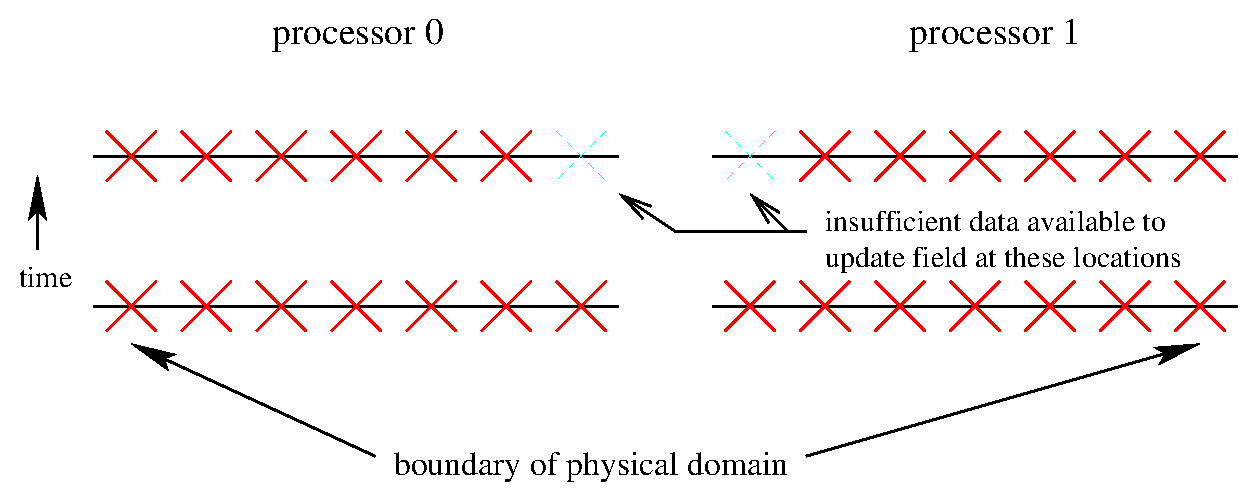
\includegraphics[angle=0,width=8cm]{1dnoghost.eps}
\fi
\end{center}
\caption{Distributed wave equation with no ghostzones}
\label{fig:noghost}
\end{figure}

At the outer boundary of the physical domain the data for the boundary
point can be generated by the boundary conditions, however at internal
boundaries the data has to be copied from the adjacent processor.  It
would be inefficient to copy each point individually, so instead, a
number of {\bf ghostzones} are created at the internal boundaries.  A
ghostzone consists of a copy of the whole plane (in 3d, line in 2d,
point in 1d) of the data from the adjacent processor.  I.e. the array
on each processor is augmented with copies of points from the adjacent
processors, thus allowing the algorithm to proceed {\bf on the points
owned by this processor} without having to worry about copying data.
Once the data has been evolved one step, the data in the ghostzones
can be exchanged (or {\bf synchronised}) between processors in one
fell swoop before the next evolution step.  (See figure
\ref{fig:withghost}.)  Note that you should have at least as many
ghostzones as your stencil-size requires.

\begin{figure}[ht]
\begin{center}
\ifpdf
\else
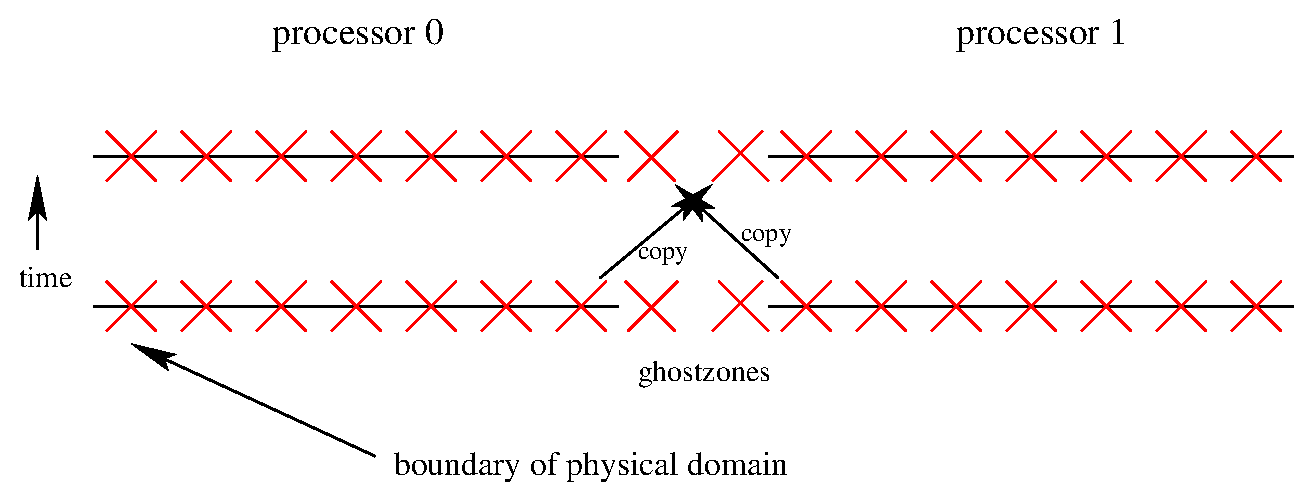
\includegraphics[angle=0,width=8cm]{withghost.eps}
\fi
\end{center}
\caption{Distributed wave equation with ghostzones}
\label{fig:withghost}
\end{figure}

\section{Staggering}

The staggering of a gridfunction or array describes the {\em physical}
placement of that gridfunction relative to the supporting grid
structure. For example, a gridfunction does not have to
be placed at the intersection
of the ``grid lines''. It can be moved by half a grid spacing in
any or all dimensions. In the latter case, it will be placed in
the center of a cell.

The staggering of grid function is a pure {\em physical} property:
the values will be calculated at a different position in physical
space. Still the indexing (or bookeeping)  is kept the same for all
types of staggerings: the indexing of the default unstaggered grids is
used.

\vskip .25cm

{\bf Specifying the staggertype}

The type of staggering applied to a gridfunction can be specified in
the {\tt interface.ccl} file by the attribute {\tt stagger} (see
\ref{sec:in}). Cactus supports three kinds of staggering
per dimension. The physical location of a gridfunction is shifted
relative to the default position by adding the following values to the
stagger attribute:
\begin{Lentry}
\item[{\tt M}] no staggering, default. Refers to the ``minus'' face
relative to  the default gridpoint.
\item[{\tt C}] centre staggering. The physical location is offset by
half of the grid spacing in the positive direction (or to the right).
\item[{\tt P}] full staggered. P refers to plus. The physical location
is offset by a full gridspacing in the positive direction (or the
right).
\end{Lentry}
For multi dimensional gridfunctions you concatenate the code
characters in xyz order. In Figure \ref{fig:stagger1} we show four different
staggerings of a two dimensional grid function. The solid black grid
circles show the default location of the grid function at the
intersections of the grid lines. In (A) we show an additional grid
function of type {\tt stagger=MC}: no staggering in x direction,
center staggered in y direction. In (B) we have  {\tt stagger=CM} and
staggering each direction ({\tt stagger=CC}) is shown in (C). The full
staggering in (D) ({\tt stagger=PP}) obeys the same rules, but is
rather unusual; it is included here for completeness.

\begin{figure}[ht]
  \def\epsfsize#1#2{0.45#1}
\begin{center}
\ifpdf
\else
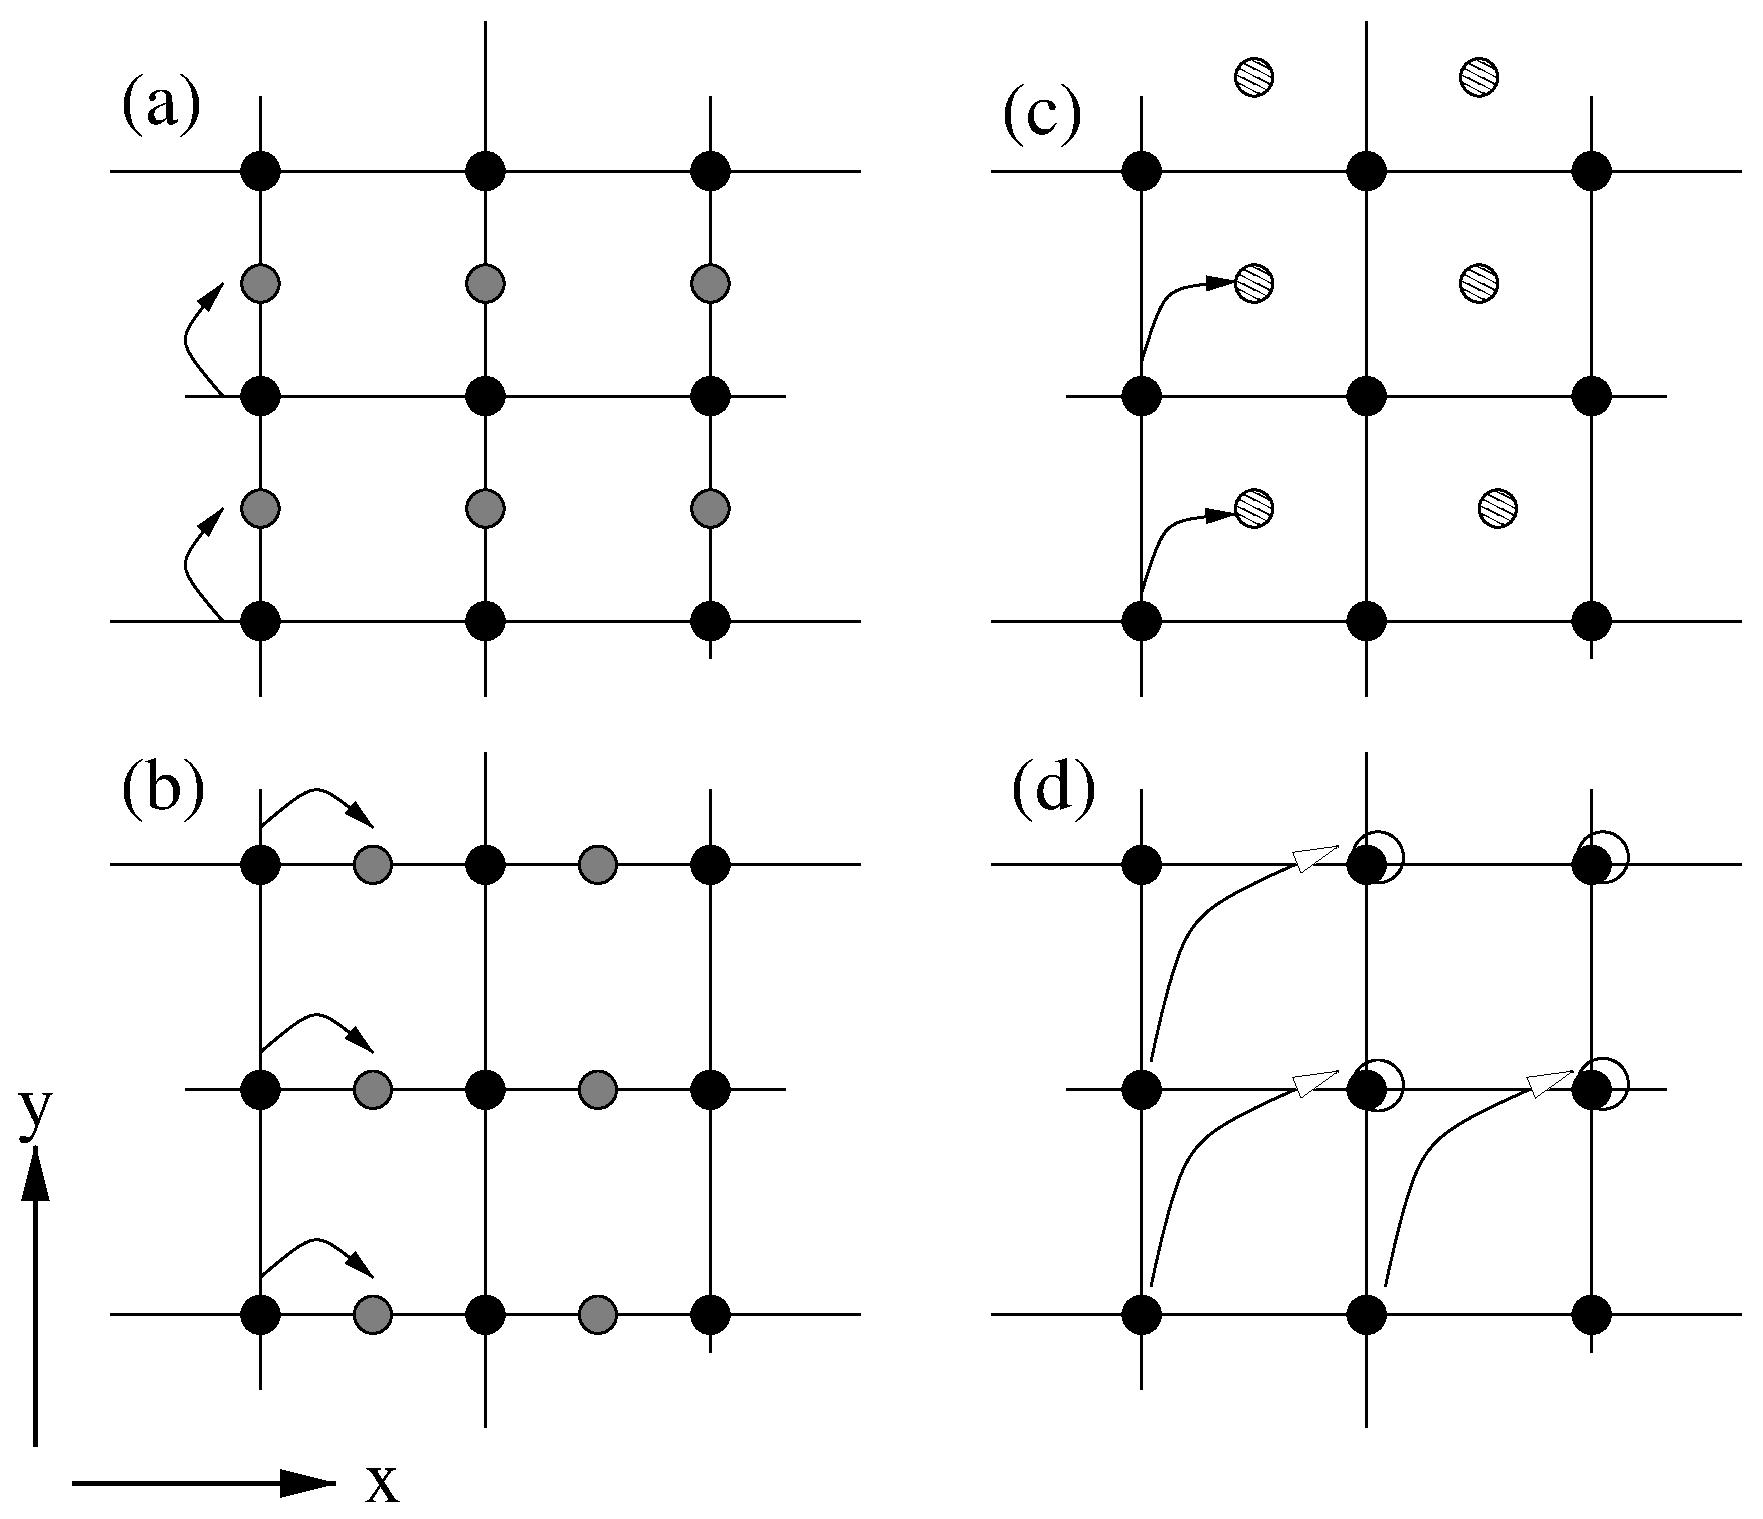
\includegraphics[angle=0,width=8cm]{staggering1.eps}
\fi
%  \centerline{\epsfbox{./staggering1.eps}}
\end{center}
\caption[]{\small {\bf Staggered gridpoints in 2D} for several
staggerings. (a) : {\tt MC}, (b): {\tt CM}, (c): {\tt CC}, (d): {\tt
PP}. Note that the staggering of gridfunctions does not change its
index. The staggered gridpoints and the corresponding unstaggered
points (arrows) are accessed by the same indices.}
\label{fig:stagger1}
\end{figure}

%%%%%%%%%%%%%%%%%%%%%%%%%%%%%%%%%%%%%%%%%%%%%%%%%%%%%%%%%%%%%%%%%%%%%%%%%%%%%%%
%%%%%%%%%%%%%%%%%%%%%%%%%%%%%%%%%%%%%%%%%%%%%%%%%%%%%%%%%%%%%%%%%%%%%%%%%%%%%%%

\chapter{Cactus Parameters}

Parameters are the means by which the user specifies the run-time behaviour of
the code.  The user specifies values for parameters in the parameter file, and
then the flesh validates these values against the ranges the thorn writers have
specified to be valid.  Once validated, parameter values are fixed, and cannot
be changed (unless the parameter is specified to be steerable, see below).

The full specification for a parameter decalaration is
\begin{verbatim}
[EXTENDS|USES] <parameter_type> <parameter name> "<parameter description>"
{
  <PARAMETER_RANGES>
} <default value>
\end{verbatim}

\section{Types and Ranges}

Parameters can be of several types:

\begin{Lentry}
\item[Integer]  Can take any integral value
\item[Real] Can take any floating point value
\item[Keyword] Can have a value consisting of one of a choice of strings
\item[Boolean] Can be true or false (1, `t', `true', or 0, `f', `false').
\item[String] Can have any string value
\end{Lentry}

Each parameter can be validated against a set of allowed values or
ranges, each of which has a description associated with it.  The type
of range is determined by the type of parameter.

\subsection{Integer}

The range specification is of the form

\begin{verbatim}

lower:upper:stride

\end{verbatim}

where {\em lower} and {\em upper} specify the lower and upper allowed
range, and {\em stride} allows numbers to be be missed out.  e.g.
\begin{verbatim}
1:21:2
\end{verbatim}
means the value must be an odd number between one and twenty-one
(inclusive).

A missing end of range (or a `*') implies negative or positive
infinity, and the default stride is one.

\subsection{Real}

The range specification is of the form
\begin{verbatim}
lower:upper
\end{verbatim}
where {\em lower} and {\em upper} specify the lower and upper allowed
range.  A missing end of range (or a `*') implies negative or positive
infinity.  The above is inclusive of the end-points.  A '(' (or ')')
before (or after) the lower (or upper) range specifies an open end-point.

\subsection{Keyword}

The range specification consists of a string, which will be matched in
a case-insensitive manner.

\subsection{Boolean}

There is no range specification for this type of parameter.

\subsection{String}

The range is a POSIX regular expression.  On some machines you may be
able to use extended regular expressions, but this is not guaranteed
to be portable.

\section{Scope}

Parameters can be {\em GLOBAL}, {\em RESTRICTED}, or {\em PRIVATE}.
Global parameters are visible to all thorns.  Restricted parameters
are visible to any thorn which chooses to {\em USE} or {\em EXTEND}
it.  A private parameter is only visible to the thorn which declares
it.


%%%%%%%%%%%%%%%%%%%%%%%%%%%%%%%%%%%%%%%%%%%%%%%%%%%%%%%%%%%%%%%%%%%%%%%%%%%%%%%
%%%%%%%%%%%%%%%%%%%%%%%%%%%%%%%%%%%%%%%%%%%%%%%%%%%%%%%%%%%%%%%%%%%%%%%%%%%%%%%

\chapter{Scheduling}
\label{chap:scheduling}

Cactus contains a rule-based scheduling system, which determines which
routines from which thorn are run in which order.  The scheduler
determines if the specifications are inconsistent, but does allow the
user to schedule a routine with respect to another routine which may not
exist.

The full specification for a schedule declaration is
\begin{verbatim}
schedule [GROUP] <function|schedule group name> AT|IN <time|schedule group name> \
                 [BEFORE|AFTER <item>] [WHILE <variable>] [AS <alias>]
{
  LANG: <language>
  [STORAGE:       <group>,<group>...]
  [TRIGGER:       <group>,<group>...]
  [SYNC:          <group>,<group>...]
  [OPTIONS:       <option>,<option>...]
} "Description of function| schedule group"
\end{verbatim}

This consists of a mandatory part, a set of options, and the main
body, referred to as the {\tt schedule block}.

Each schedule item is scheduled either {\em AT} a particular {\em
scheduling bin}, or {\em IN} a schedule {\em group}.

\section{Schedule Bins}
\label{scheduling:schedule_bins}

These are the main points at which scheduled functions are run.
These are listed in \ref{subsec:schedule_ccl}.

\section{Groups}
\label{scheduling:groups}

If the optional {\tt GROUP} specifier is used, the item is a schedule
group rather than a normal function.  Schedule groups are effectively
new, user-defined, schedule bins.  Functions or groups may be
scheduled {\em IN} these in the same way as they are scheduled {\em
AT} the main schedule bins.  (I.e. groups may be nested.)

\section{Schedule Options}
\label{scheduling:schedule_options}
The options define various charactertics of the schedule item.

\begin{Lentry}
\item[{\tt BEFORE or AFTER}]
These specify a function or group before or after which this item will
be scheduled.
\item[{\tt WHILE}]
This specifies a {\em CCTK\_INT} grid scalar which is used to control
the execution of this item.  If the grid scalar has a non-zero value
the schedule item will be executed, otherwise the item will be
ignored.  This allows iteration within the scheduler.
\item[{\tt AS}]
This assigns a new name to a function for scheduling purposes.  This
is used, for instance, to allow a thorn to schedule something before
or after a routine from another implementation;  two thorns providing this
implementation can schedule a routine {\em AS} the same thing, thus
allowing other thorns to operate independently of which one is active.
\end{Lentry}

\section{The Schedule Block}
\label{scheduling:schedule_block}

The schedule block specifies further details of the scheduled function
or group.

\begin{Lentry}
\item[\texttt{LANG}]
This specifies the language of the routine.  Currently this is either
C or Fortran.
\item[\texttt{STORAGE}] The {\tt STORAGE} keyword specifies groups for
which memory should be allocated for the duration of the routine or
schedule group.  The storage status reverts to its previous status
after completion of the routine or schedule group.
\item[\texttt{TRIGGER}]
This is only used for items scheduled at {\em CCTK\_ANALYSIS}.  The
item will only be executed if output is due for at least one
variable in one of the listed groups.
\item[\texttt{SYNC}]
On exit from this item the ghost zones of the listed groups will be
exchanged.
\item[\texttt{OPTIONS}]
This is for miscellaneous options.  The only currently supported
option is {\em GLOBAL} which tells the driver that this routine does
not use a local grid, but instead uses global operations to process
data;  such a routine should only be called once however many
sub-grids the driver may have broken the problem into.
\end{Lentry}

\section{How Cactus Calls Scheduled Functions}
\label{scheduling:calling_scheduled_functions}

For each scheduled function called, the flesh performs a variety of jobs at entry and exit.

On entry to a scheduled routine, if the routine is being called at the ANALYSIS timebin first a check is made to see if the routine should actually be called on this timestep. For this, all grid variables in the trigger groups for the routine are checked with all registered output methods to determine if it is time to output any triggers. The routine will only be called if at least one is due to be output. Routines from all other timebins are always called.

Next storage is assigned for any required variables, remembering the original state of storage.

The routine is then called, and on exit, any required grid variables are
first synchronised. Following synchronization, any required output methods are called for the triggers. Finally, the storage of grid variables is returned to the original state.

%%%%%%%%%%%%%%%%%%%%%%%%%%%%%%%%%%%%%%%%%%%%%%%%%%%%%%%%%%%%%%%%%%%%%%%%%%%%%%%
%%%%%%%%%%%%%%%%%%%%%%%%%%%%%%%%%%%%%%%%%%%%%%%%%%%%%%%%%%%%%%%%%%%%%%%%%%%%%%%

\chapter{Writing a Thorn}

\section{Thorn Programming Languages}

When you start writing a new thorn, the first decision to make is
which programming language to use? The source code in Cactus thorns
can be written in any mixture of {\tt FORTRAN77}, {\tt FORTRAN90},
{\tt C} or {\tt C++}. The following points should be considered when
choosing a language to work in
\begin{itemize}

\item All functions designed for application thorn writers are available
      in all languages, however some interfaces for infrastructure
      thorn writing are only available from {\tt C} or {\tt C++}.

% This is no longer relevant?
%\item If you are writing in {\tt FORTRAN}, use {\tt F77} if you want
%      to distribute your code to people who may not be able to afford
%      to buy proprietory {\tt F90} compilers.

\item Stick to {\tt C} rather than {\tt C++}, unless you really need
      features from {\tt C++}, this will help you with portability.

\end{itemize}

Whatever language you choose, if you want your thorn to be portable, and
compile and run on multiple platforms, stick to the standards and don't
use machine dependent extensions.


\section{What the Flesh provides}

The flesh provides for thorns:
\begin{Lentry}
\item [{\tt Variables}]
\item [{\tt Parameters}]
\item [{\tt Cactus Functions}]

\begin{itemize}
  \item{} driver (parallelisation) utilities
  \item{} IO utilities
  \item{} Coordinates utilities
  \item{} Reduction utilities
  \item{} Interpolation utilities
  \item{} Information utilities
\end{itemize}
\end{Lentry}


\subsection{Fortran Routines}

Any source file using Cactus infrastructure should include
the header file {\tt cctk.h} using the line
\begin{verbatim}
#include "cctk.h"
\end{verbatim}
(Fortran programmers should not be put of by this being a C style
header file, most Cactus files are run through a C preprocessor
before compilation).

\subsubsection{Variables}

Any routine using Cactus argument lists (for example all
routines called from the scheduler) should include at the
top of the file the header
\begin{verbatim}
#include "cctk_Arguments.h"
\end{verbatim}

A Cactus macro {\tt CCTK\_ARGUMENTS} is defined for each thorn
to contain:
\begin{itemize}
\item General information about the grid hierarchy, for example
      the number of grid points used. See Section \ref{sec:cava2} for a
      complete list.
\item All the grid variables defined in the thorn's {\tt interface.ccl}
\item All the grid variables required from other thorns as requested by
      the {\tt inherits} and {\tt friend} lines in the {\tt interface.ccl}
\end{itemize}
These variables must be declared at the start of the routine using
the macro {\tt DECLARE\_CCTK\_ARGUMENTS}.

To pass the arguments to another routine in the same thorn use the macro
{\tt CCTK\_PASS\_FTOF} in the calling routine, and again the macro
{\tt CCTK\_ARGUMENTS} in the receiving routine.


\subsubsection{Parameters}

All parameters defined in a thorn's {\tt param.ccl} and all {\tt global}
parameters appear as local variables of the corresponding CCTK datatype
in Fortran source code, ie. Booleans and Integers appear as CCTK\_INT types
(with non-zero/zero values for boolean {\t yes/no}),
Reals as CCTK\_REAL, and Keywords and String parameters as CCTK\_POINTER (see
also note below). These variables are {\tt read only} and {\em changes should
not be made to them}. The effect of changing a parameter is undefined (at best).

Any routine using Cactus parameters should include at
the top of the file the header
\begin{verbatim}
#include "cctk_Parameters.h"
\end{verbatim}

The parameters should be declared at the start of the routine
using them with the macro {\tt DECLARE\_CCTK\_PARAMETERS}.

In Fortran, special care should be taken with string valued parameters.
These parameters are passed as C pointers, and can not be treated as
normal Fortran strings. 
To compare a string valued parameter and Fortran
string use the macro {\tt CCTK\_EQUALS()} or the function {\tt CCTK\_Equals()}.
To print the value of a string valued parameter to screen, use the subroutine
{\tt CCTK\_PrintString()}. A further function {\tt CCTK\_FortranString} 
provides a mechanism for converting a string parameter to a Fortran string. 
For example, if {\tt operator} is a Cactus string parameter holding the name of a reduction operator whose handle you need to find, you cannot pass it 
directly into the subroutine {\tt CCTK\_ReductionHandle} which is expecting 
a Fortran string. Instead, the following is needed:
{\tt
\begin{verbatim}
      character*200 fortran_operator
      CCTK_INT      fortran_operator_len
      integer       handle

      call CCTK_FortranString(fortran_operator_len,operator,fortran_operator)
      call CCTK_ReductionHandle(handle,fortran_operator(1:fortran_operator_len))
\end{verbatim}
}



\subsubsection{Fortran Example}

The Fortran routine {\tt MyFRoutine} is scheduled in the {\tt schedule.ccl} file,
doesn't use Cactus parameters, and calls another routine, in the same thorn,
{\tt MyNewRoutine} which does use parameters.
This routine needs to be passed an integer flag as
well as the standard Cactus variables. The source file should look like

\begin{verbatim}
#include "cctk.h"
#include "cctk_Arguments.h"
#include "cctk_Parameters.h"

      subroutine MyFRoutine(CCTK_ARGUMENTS)

c     I'm very cautious, so I want to declare all variables
      implicit none

      DECLARE_CCTK_ARGUMENTS

      integer flag

      flag = 1
      call MyNewRoutine(CCTK_PASS_FTOF,flag)

      return
      end

      subroutine MyNewRoutine(CCTK_ARGUMENTS,flag)

      implicit none

      DECLARE_CCTK_ARGUMENTS
      DECLARE_CCTK_PARAMETERS
      integer flag

c     Main code goes here

      return
      end

\end{verbatim}

\subsubsection{Cactus Fortran Functions}

Cactus Fortran functions, for example {\tt CCTK\_MyProc()} and {\tt
CCTK\_Equals}, can all be declared by adding before any executable code, the
declaration

\begin{verbatim}
DECLARE_CCTK_FUNCTIONS
\end{verbatim}

\subsubsection{Fortran 90 Modules}

Fortran 90 modules should be included in a thorn's {\tt make.code.deps} file
(\ref{sec:mabathbu}) to ensure they are compiled before the
routines which use them. This is especially important for parallel
building. For example, if a routine in {\tt MyRoutine.F} uses a module
in {\tt MyModule.F} add the line:
{\tt
\begin{verbatim}
$(SYS_OBJD)/MyRoutine.F.o:         $(SYS_OBJD)/MyModule.F.o
\end{verbatim}
}

\subsubsection{The {\tt MOD} function}

The intrinsic function {\tt MOD} in Fortran takes two integer
arguments, which should both be of the same type. This means
that it may be necessary to cast the arguements to {\it e.g}
{\tt INT} for some architectures. This can occur in particular
when a {\tt CCTK\_INT} parameter and the Cactus variable {\tt cctk\_iteration}
(which is declared to be {\tt INTEGER}) are used,
in which case the correct code is
\begin{verbatim}
MOD(cctk_iteration,INT(MyParameter))
\end{verbatim}


\subsection{C Routines}

Any source file using Cactus infrastructure should include
the header file {\tt cctk.h} using the line
\begin{verbatim}
#include "cctk.h"
\end{verbatim}

\subsubsection{Variables}

Any routine using Cactus argument lists (for example all
routines called from the scheduler) should include at the
top of the file the header
\begin{verbatim}
#include "cctk_Arguments.h"
\end{verbatim}

A Cactus macro {\tt CCTK\_ARGUMENTS} is defined for each thorn
to contain
\begin{itemize}
\item General information about the grid hierachy, for example the
number of grid points on the processor. See Section \ref{sec:cava2}
for a complete list.
\item All the grid variables defined in the thorn's {\tt interface.ccl}
\item All the grid variables required from other thorns as requested by
      the {\tt inherits} and {\tt friend} lines in the {\tt interface.ccl}
\end{itemize}
These variables must be declared at the start of the routine using
the macro {\tt DECLARE\_CCTK\_ARGUMENTS}. This macro should always be the
first line of the routine.

To pass the arguments to another routine in the same thorn use the macro
{\tt CCTK\_PASS\_CTOC} in the calling routine, and again the macro
{\tt CCTK\_ARGUMENTS} in the receiving routine.


\subsubsection{Parameters}

All parameters defined in a thorn's {\tt param.ccl} and all {\tt global}
parameters appear as local variables of the corresponding CCTK datatype
in C source code, ie. Integers and Booleans appear as CCTK\_INT types (with
non-zero/zero values for boolean {\t yes/no)}, Reals as
CCTK\_REAL, and Keywords and String parameters as CCTK\_STRING.
These variables are {\tt read only} and {\em changes should not be made to
them}.  The effect of changing a parameter is undefined (at best).

Any routine using Cactus parameters should include at
the top of the file the header
\begin{verbatim}
#include "cctk_Parameters.h"
\end{verbatim}

The parameters should be declared as the last statement in the declaration part
of the routine using them with the macro {\tt DECLARE\_CCTK\_PARAMETERS}.

\subsubsection{Example}

The C routine ``MyCRoutine'' is scheduled in the {\tt schedule.ccl} file,
and uses Cactus parameters. The source file should look like
\begin{verbatim}
#include "cctk.h"
#include "cctk_Arguments.h"
#include "cctk_Parameters.h"

void MyCRoutine(CCTK_ARGUMENTS)
{
  DECLARE_CCTK_ARGUMENTS
  DECLARE_CCTK_PARAMETERS

  /* Here goes your code */
}
\end{verbatim}

\subsubsection{Complex variables}

Cactus supports complex grid variables, and since there is no
complex data type in C, Cactus provides a number
of functions for manipulating complex numbers to mirror the
functionality available in Fortran. These functions are {\tt CCTK\_Cmplx},
{\tt CCTK\_CmplxReal}, {\tt CCTK\_CmplxImag}, {\tt CCTK\_CmplxConjg},
{\tt CCTK\_CmplxAdd}, {\tt CCTK\_CmplxSub}, {\tt CCTK\_CmplxMul},
{\tt CCTK\_CmplxDiv}, {\tt CCTK\_CmplxExp}, {\tt CCTK\_CmplSin},
{\tt CCTK\_CmplxAbs}, {\tt CCTK\_CmplxLog}, and {\tt CCTK\_CmplSqrt}.


\subsubsection{Specifically for C Programmers}

Grid functions are held in memory as 1D C arrays. These are laid
out in memory as in Fortran. This means that the first index should
be incremented through most rapidly.  This is illustrated in the example
below.

Cactus provides
macros to find the 1D index which is needed from the multidimensional
indices which are usually used. There is a macro for each dimension of
grid function.  Below is an articifial example to demonstrate this
using the 3D macro {\tt CCTK\_GFINDEX3D}:
\begin{verbatim}
for (k=0; k<cctk_lsh[2]; k++)
{
  for (j=0; j<cctk_lsh[1]; j++)
  {
    for (i=0; i<cctk_lsh[0]; i++)
    {
      My3D_GF[CCTK_GFINDEX3D(cctkGH,i,j,k)] = i*j*k;
    }
  }
}
\end{verbatim}
%
Here, {\tt CCTK\_GFINDEX3D(cctkGH,i,j,k)]} expands to
\begin{verbatim}
((i) + cctkGH->cctk_lsh[0]*((j)+cctkGH->cctk_lsh[1]*(k)))
\end{verbatim}

\subsection{Cactus Variables}
\label{sec:cava2}

The Cactus variables which are passed through the macro
{\tt CCTK\_ARGUMENTS} are
\begin{Lentry}
\item [{\tt cctk\_dim}] An integer with the number of dimensions
      used for this grid hierarchy.
\item [{\tt cctk\_lsh}] An array of {\tt cctk\_dim} integers
      with the local grid size on this processor.
\item [{\tt cctk\_gsh}] An array of {\tt cctk\_dim} integers
      with the {\it global} grid size.
\item [\texttt{cctk\_iteration}] The current iteration number.
\item [{\tt cctk\_delta\_time}] A {\tt CCTK\_REAL} with the timestep.
\item [{\tt cctk\_time}] A {\tt CCTK\_REAL} with the current time.
\item [{\tt cctk\_delta\_space}] An array of {\tt cctk\_dim} {\tt
CCTK\_REAL}s with the grid spacing in each direction.
\item [{\tt cctk\_nghostzones}] An array of {\tt cctk\_dim} integers with
         the number of ghostzones used in each direction.
\item [{\tt cctkGH}] A C pointer identifying the grid hierachy.
%\item [{\tt cctk\_from}] The index value from which the user should start loops.
%\item [{\tt cctk\_to}] ... end loops.
%\item [{\tt cctk\_origin\_space}]  The coordinates of the spatial origin?
%\item [{\tt cctk\_lssh}]  This is an internal array used to hold array extents for staggering.  One should use the macro CCTK_LSSH(,) to access its elements.
\end{Lentry}

The following variables describe the location of the local
grid (e.g. the grid treated on a given processor) within
the global grid.
\begin{itemize}
\item {\tt cctk\_lbnd}
      An array of {\tt cctk\_dim} integers
      containing the lowest index (in each direction)
      of the local grid, as seen on the global grid. Note that these indices
      start from zero, so you need to add one when using them in
      Fortran thorns.
\item {\tt cctk\_ubnd}
      An array of {\tt cctk\_dim} integers
      containing the largest index (in each direction)
      of the local grid, as seen on the global grid.  Note that these indices
      start from zero, so you need to add one when using them in
      Fortran thorns.
\item {\tt cctk\_bbox}
      An array of 2*{\tt cctk\_dim} integers (in the order
	$[{\mbox{dim}}_0^{\mbox{min}}, \mbox{dim}_0^{\mbox{max}},
	{\mbox dim}_1^{\mbox{min}}, {\mbox dim}_1^{\mbox{max}}, \ldots]$),
      which indicate whether the boundaries are internal boundaries
      (e.g. between processors), or physical boundaries. A value of 1 indicates
      a physical (outer) boundary at the edge of the computational grid,
      and 0 indicates an internal boundary.
\end{itemize}

The following variable is needed for grid refinement methods
\begin{itemize}
\item {\tt cctk\_levfac} The factor by which the local grid is refined
        with respect to the base grid.
\end{itemize}

The following variable is used for identifing convergence levels. {\tt NOTE:} Convergence is not currently implemented by Cactus, so that {\tt cctk\_convlevel} is currently always 0.
\begin{itemize}
\item {\tt cctk\_convlevel} The convergence level of this grid hierachy.
 	The base level is 0, and every level above that is currently coarsened 	       by a factor of 2.
\end{itemize}

The variables {\tt cctk\_delta\_space} and {\tt cctk\_delta\_time}
denote the grid spacings on the {\em base} grid. If you are using
a grid refinement method, you need to calculate the grid spacings
on the grid you are on. There are Cactus macros provided for this,
with the syntax {\tt CCTK\_DELTA\_SPACE(dir)} and {\tt CCTK\_DELTA\_TIME}
for both C and Fortran. It is recommended that these macros are
always used to provide the grid spacings in your thorns.

\subsection{Cactus Data Types}

The Cactus grid variables and parameters are defined and
declared using Cactus data types, to provide portability
across platforms. The most important of
these data types are described below, for a full description
see Section~\ref{sec:datyansi}. These data types should
be used to declare local variables where needed, and to
declare Cactus grid variables or parameters that need
declarations.

\begin{Lentry}

\item[{\tt CCTK\_INT}] default size 4 bytes
\item[{\tt CCTK\_REAL}] default size 8 bytes

\end{Lentry}

\subsubsection{Example}

In the following example {\tt MyScalar} is a grid scalar which
is declared in the {\tt interface.ccl} as {\tt CCTK\_REAL}.

\begin{verbatim}
      subroutine InitialData(CCTK_ARGUMENTS)

      DECLARE_CCTK_ARGUMENTS

      CCTK_REAL local_var

      local_var = 1.0/3.0
      MyScalar = local_var

      return
      end
\end{verbatim}

Declaring {\tt local\_var} to have a non-Cactus data type, e.g.
{\tt REAL*4}, or using one of the other Cactus real data types
described in Section~\ref{sec:datyansi} could give problems for
different architectures or configurations.

\subsection{Staggering}
\label{sec:st}

{\bf Indexing, ghostzones, etc.}
Note that staggering does not make any changes to the indexing of a
gridfunction: the black solid circles in diagram \ref{fig:stagger2} and their
associated staggered gridfunctions (connected by arrows) have the same index!

Since the gridfunction does not ``know'' anything about the physical
location (it's only addressed by indices) why add staggering if the
indexing is the same?

Indeed, you could roll your own, but there compelling reasons:
Readabilty and the fact that you are able to query the staggertype of a
gridfunction. More important: in the way the grid is laid out, there is one grid
point {\em less} for {\tt M} and {\tt P} staggered grid functions. This is
illustrated in picture \ref{fig:stagger2}, which shows 15 gridpoints distributed
across 3 processors. The solid black circles show the default
location of the gridfunctions, the grey circles depict the ghostzones.
Note that the number of center staggered gridpoints (fat crosses)
corresponds to the number of default gridpoints on all processors but
the last one. (The same is true for full staggered gridpoints).

{\bf Staggertypes}
The string specifying the staggering is encoded in a number called
the {\em staggerindex}. With the 3 supported staggerings, the string
is converted into a base-3 number. Several routines exist, to extract the
staggering in a specific direction, called {\em directional
staggerindex}. E.g. {\tt stagger = MCM}: {\em staggerindex} = 3, in the
x-direction: {\em directional staggerindex} = CCTK\_STAGGER\_M (value 0),  in the
x-direction: {\em directional staggerindex} = CCTK\_STAGGER\_C (value 1).

\begin{Lentry}
\item[{\tt CCTK\_STAGGER\_M}]  value used for M-type staggering
\item[{\tt CCTK\_STAGGER\_C}]  value used for C-type staggering
\item[{\tt CCTK\_STAGGER\_P}]  value used for P-type staggering
\item[{\tt CCTK\_NO\_STAGGER}] value to indicate no staggering
\item[{\tt CCTK\_STAGGER}]    value to indicate staggering
\item[{\tt CCTK\_NSTAGGER}]   number of coded staggerings (3)
%\item[{\tt CCTK\_STAGGER\_ERROR}] failed stagger operation, negative
\end{Lentry}


\begin{figure}[ht]
  \def\epsfsize#1#2{0.45#1}
\begin{center}
\ifpdf
\else
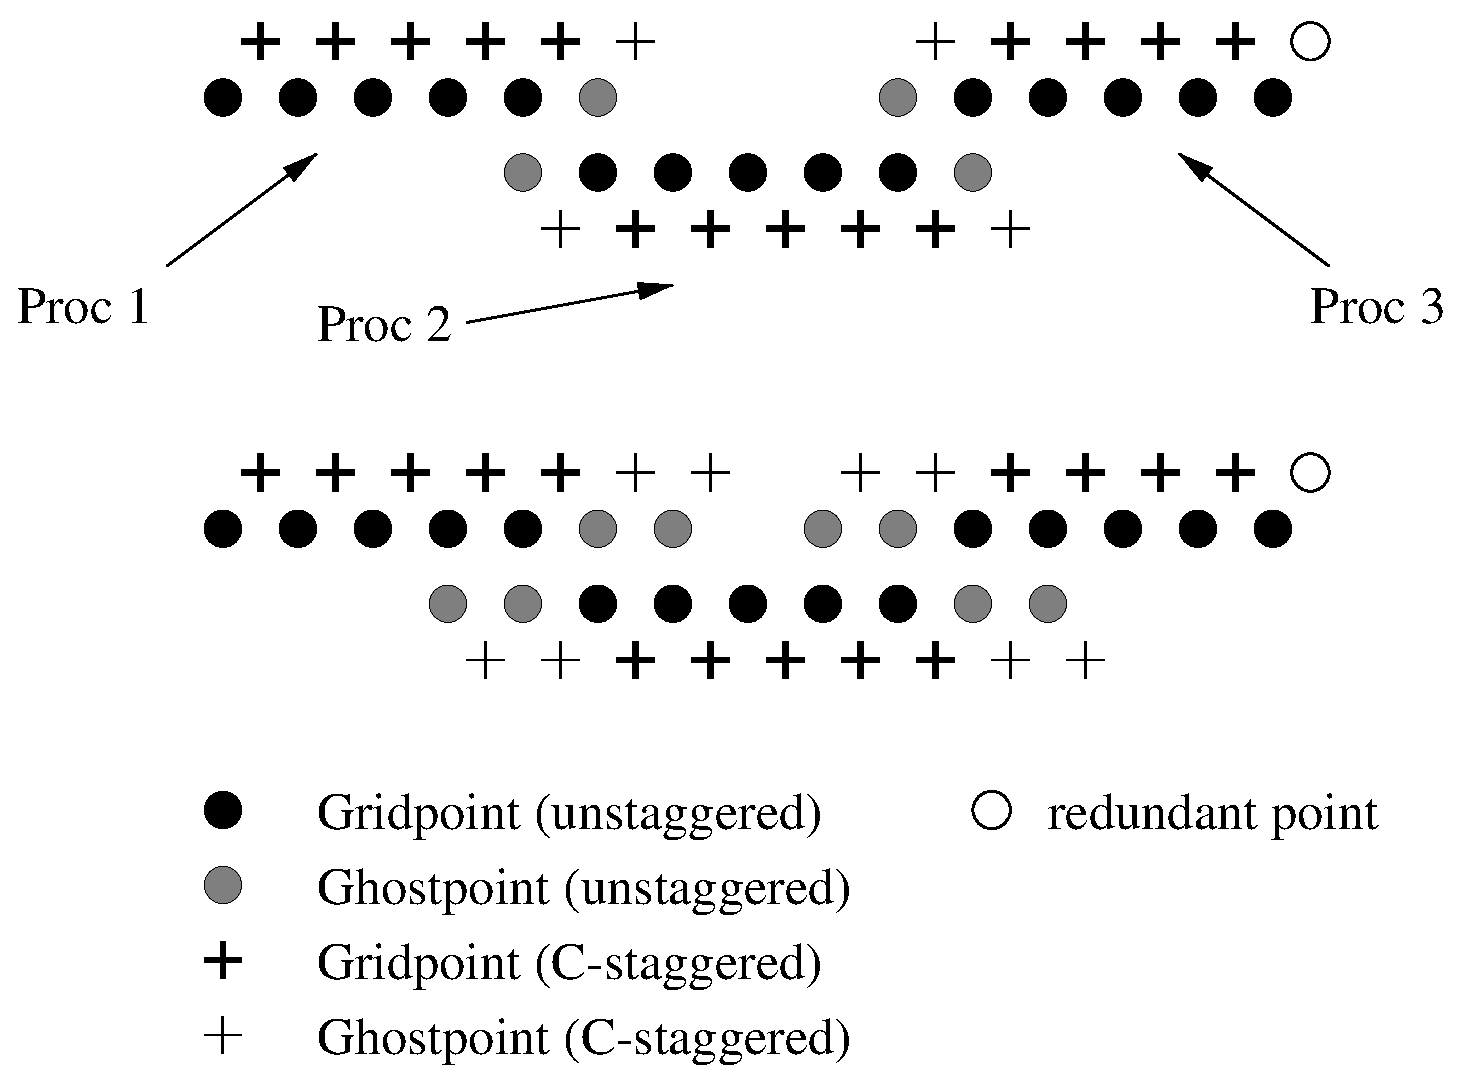
\includegraphics[angle=0,width=10cm]{staggering2.eps}
\fi
%  \centerline{\epsfbox{./staggering2.eps}}
\end{center}
\caption[]{\small {\bf Unstaggered and center-staggered gridpoints} with
ghostzone size of one (above) and two (below). The points are
distributed across three processors. Note that the number of
center staggered gridpoints (fat crosses) is one less on the outermost grid. How to
treat this case in a easy way is explained below. }
\label{fig:stagger2}
\end{figure}

When a thorn programmer uses staggered gridpoints, he has to be aware
of this gridpoint anomaly. This can be done most easily by using the {\tt
CCTK\_LSSH(<dir\_staggertype>,<direction>)} macro. For a given staggertype
and direction, this 2d array returns the local number of gridpoints,
including  ghostzones and the necessary change for the staggering on
the outermost processor.

\begin{Lentry}
\item[{\tt CCTL\_LSSH(<dir\_staggertype>,<direction>)}]
for a given staggertype and a direction this macro returns the number
of processor local gridpoints, including ghostzones.

\begin{itemize}
\item{macro has to be in capital letters}
\item{This macro is C/Fortran indexing aware:
can specify the dimension in C ranging from $0 \ldots$ and in Fortan
ranging from $1 \ldots$.}
\end{itemize}
\end{Lentry}

\vskip .25cm

Several functions exist to derive the staggertype for a given group
and for a certain direction.
\begin{Lentry}
\item[{\tt int CCTK\_GroupStaggerIndexGI(int group\_index)}] %returns the
%{\em staggerindex} for a given group index.
\item[{\tt call CCTK\_GroupStaggerIndexGI(int staggerindex, int
group\_index)}]  returns the {\em staggerindex} for a given group index.
\end{Lentry}
\vskip .45cm

\begin{Lentry}
\item[{\tt int CCTK\_GroupStaggerIndexGN(char *group\_name)}] %returns the
%{\em staggerindex} for a given group name.
\item[{\tt call CCTK\_GroupStaggerIndexGN(int staggerindex, char *group\_name)}] returns the
{\em staggerindex} for a given group name. \vskip .25cm
\end{Lentry}
\vskip .45cm

\begin{Lentry}
\item[{\tt int CCTK\_GroupStaggerIndexVI(int variable\_index)}] %returns the
%{\em staggerindex} for a given variable index.
\item[{\tt call CCTK\_GroupStaggerIndexVI(int staggerindex, int variable\_index)}] returns the
{\em staggerindex} for a given variable index.
\end{Lentry}
\vskip .45cm

\begin{Lentry}
\item[{\tt int CCTK\_GroupStaggerIndexVN(char *variable\_name)}] %returns the
%{\em staggerindex} for a given variable name.
\item[{\tt call CCTK\_GroupStaggerIndexVN(int staggerindex, char *variable\_name)}] returns the
{\em staggerindex} for a given variable name.
\end{Lentry}
\vskip .45cm

\begin{Lentry}
\item[{\tt int CCTK\_StaggerIndex(char *stagger\_string)}] %return the {\em
%staggerindex} for a given stagger string.
\item[{\tt call CCTK\_StaggerIndex(int staggerindex, char *stagger\_string)}] return the {\em
staggerindex} for a given stagger string.
\end{Lentry}
\vskip .45cm

\begin{Lentry}
\item[{\tt int CCTK\_DirStaggerIndex(int direction, char *stagger\_string)}]
%returns the {\em directional staggerindex} for a given direction and
%stagger string.
\item[{\tt call CCTK\_DirStaggerIndex(int dir\_staggerindex, int direction, char *stagger\_string)}]
returns the {\em directional staggerindex} for a given direction and
stagger string.
\end{Lentry}
\vskip .45cm

\begin{Lentry}
\item[{\tt int CCTK\_DirStaggerIndexI(int direction, char *stagger\_type)}]
%returns the {\em directional staggerindex} for a given direction and
%staggerindex.
\item[{\tt call CCTK\_DirStaggerIndexI(int dir\_direction, char *stagger\_type)}]
returns the {\em directional staggerindex} for a given direction and
staggerindex.

\end{Lentry}


\section{Parallelisation}
\label{seap}

The flesh itself does not actually set up grid variables. This
is done by a {\it driver} thorn. To allow the distribution of
a grid over a number of processors, the driver thorn must
also provide the grid decomposition, and routines to enable
parallelisation. The method used to provide this parallelisation
(e.g. MPI, PVM) is not usually important for the thorn writer since
the driver thorn provides routines which are called by standard interfaces
from the flesh. Here we describe briefly the most important of these routines
for the application thorn writer. A more detailed description
of these interfaces with their arguments, is given in the Function Reference
Guide.
A complete description of the
routines a driver thorn must provide will be provided in the
Interface Thorn Writers guide. The standard driver thorn is
currently {\tt PUGH} in the {\tt CactusPUGH} package, which
is a parallel unigrid driver.

\begin{Lentry}
\item[{\tt CCTK\_nProcs}] Returns the number of processors being used
\item[{\tt CCTK\_MyProc}] Returns the processor number (this starts at
  processor number zero)
\item[{\tt CCTK\_SyncGroup}] Synchronises a group of variables by
  exchanging the values held in each processor ghostzones with the
  physical values of their neighbours
\item[{\tt CCTK\_Barrier}] Waits for all processors to reach this point
  before proceeding
\end{Lentry}

\chapter{Cactus Application Interfaces}


\section{Coordinates}
\label{sec:co}

The flesh provides utility routines for registering and querying
coordinate information. The flesh does not provide any coordinates
itself, these must be supplied by a thorn. Thorns are not required to
register coordinates to the flesh, but registering coordinates
provides a means for infrastructure thorns to make use of coordinate
information.

Coordinate support is still being developed in the Cactus flesh. At
the moment, it is assumed that coordinates will usually be grid
functions.

Coordinates are grouped into {\it coordinate systems}, which have a
specified dimension. Any number of coordinate systems can be
registered with the flesh, and a coordinate system must be registered
before any coordinates can be registered, since they must be
associated with their corresponding system.  Coordinates can be
registered, with any chosen name, with an existing coordinate system,
along with their direction or index in the coordinate system.
Optionally, the coordinate can also be associated with a given grid
variable.  A separate call can register the global range for a
coordinate on a given grid hierarchy.

Following conventions for coordinate system and coordinate names
provides a means for other thorns to use the physical properties of
coordinate systems, without being tied to a particular thorn.

A registered coordinate system can be refered to by both its name and
an associated handle. Passing such an integer handle instead of the
name string may be necessary for calling C routines from Fortran.

\subsection{Registering Coordinates and Coordinate Properties}

Coordinate systems and their properties can be registered at any time with the Flesh.
The registration utilities for thorns providing coordinates are:
\begin{Lentry}

\item[{\tt CCTK\_CoordRegisterSystem}]

Assigns a coordinate system with a chosen name and dimension. For example,
a 3-dimensional Cartesian coordinate system could be registered with the
name {\tt cart3d} using the call from C

{\tt
int ierr;\\
int dim=3;\\
ierr = CCTK\_CoordRegisterSystem(dim,"cart3d");
}

\item[{\tt CCTK\_CoordRegisterData}]

Defines a coordinate in a given coordinate system, with a given
	direction and name, and optionally associates it to a grid variable.
The directions of the coordinates range from 1 to the dimension of the
coordinate system. For example, to register the grid variable {\it grid::y3d}
to have the coordinate name {\tt y} in the {\tt cart3d} system

{\tt
int ierr;\\
int dir=2;\\
ierr = CCTK\_CoordRegisterData(dir,"grid::y3d","y","cart3d");
}

\item[{\tt CCTK\_CoordRegisterRange}]

Assigns the global computational maximum and minimum for a coordinate
on a grid hierachy, that is in a {\tt cctkGH}. At this time the
maximum and minimum values have to be of type {\tt CCTK\_REAL}. For
example, if the {\tt y} coordinate for the {\tt cart3d} system ranges
between zero and one

{\tt
CCTK\_REAL lower=0;\\
CCTK\_REAL upper=1;\\
int ierr;\\
ierr = CCTK\_CoordRegisterRange(cctkGH, lower, upper, -1, "y", "cart3d");
}

Note that the API allows either the coordinate name or the direction to
be used, so that the following is also valid

{\tt
CCTK\_REAL lower=0;\\
CCTK\_REAL upper=1;\\
int ierr;\\
ierr = CCTK\_CoordRegisterRange(cctkGH, lower, upper, 2, NULL, "cart3d");
}

\item[{\tt CCTK\_CoordRegisterPhysIndex}]

Implementing such things as symmetry properties for a grid leads to
the need to know the details of the {\it physical} section of a grid.
Such information is typically needed by IO thorns. The following call
illustrates how To register the
indices 3 and 25 as supplying the physical range of the {\tt y}
coordinate in the {\tt cart3d} system

{\tt
int loweri=3;\\
int upperi=25;\\
int ierr;\\
ierr = CCTK\_CoordRegisterPhysIndex(cctkGH, loweri, upperi, -1, "y", "cart3d");
}



\end{Lentry}

\subsection{Using Coordinates}

The utilities for thorns using coordinates are:

\begin{Lentry}

\item[{\tt CCTK\_NumCoordSystems}]

Returns the number of coordinate systems registered with the Flesh. For example,

{\tt int num;\\
num = CCTK\_NumCoordSystems();
}

\item[{\tt CCTK\_CoordSystemName}]

Provides the name of a registered coordinate system, given the integer
handle (or index) for the system in the Flesh's coordinate data base.
Note that the handle ranges between zero and the number of coordinate systems minus one: $0 \le \mbox{handle} \le \mbox{\tt CCTK\_NumCoordSystems()}-1$.
It is important to remember that the handle given to a coordinate system
depends on the order in which systems are registered, and can be different
from one simulation to the next.

For example, to print the names of all registered coordinate systems:

{\tt for (i=0; i<CCTK\_NumCoordSystems(); i++) \\
 printf("\%s ",CCTK\_CoordSystemNName(i));}

\item[{\tt CCTK\_CoordSystemDim}]

Provides the dimension of a coordinate system. For example, if
the {\tt cart3d} system was registered as having 3 dimensions, the
variable {\tt dim} below will now be set to 3,

{\tt int dim;\\
dim = CCTK\_CoordSystemDim("cart3d");
}

\item[{\tt CCTK\_CoordSystemHandle}]

Provides the integer handle for a given coordinate system name. The handle describes
the index for the coordinate system in the Flesh coordinate database, and its value
will range between zero and the number of registered systems minus one. For example,
the handle for the {\tt cart3d} coordinate system can be found using

{\tt int handle;\\
handle = CCTK\_CoordSystemHandle("cart3d");}

\item[{\tt CCTK\_CoordSystemName}]

The inverse to the previous function call, this provides the name for a given coordinate system handle.
For example to find the first coordinate system in the Flesh database

{\tt int handle = 0;\\
const char *name = CCTK\_CoordSystemName(handle);
}

\item[{\tt CCTK\_CoordIndex}]

Provides the grid variable index for a given coordinate. Notethat it is
not necessary for a registered coordinate to have an associated grid variable,
and if no such grid variable is found a negative integer will be returned.
For example, to find the grid variable index associated with the {\tt y}
coordinate of the {\tt cart3d} system, either of the two following
calls could be made

{\tt int index;\\
index = CCTK\_CoordIndex(2,NULL,"cart3d");}

{\tt int index;\\
index = CCTK\_CoordIndex(-1,"y","cart3d");}


\item[{\tt CCTK\_CoordDir}]

Provides the direction for a given coordinate. Directions are integers
ranging from one to the number of dimensions for the coordinate system.
For example, to return the direction of the {\tt y} coordinate in
the {\tt cart3d} system

{\tt int dir;\\
dir = CCTK\_CoordDir("y","cart3d");
}

The return of a negative integer indicates that the coordinate direction
could not be found.

\item[{\tt CCTK\_CoordRange}]

Provides the global range (that is, the minumum and maximum values across
the complete grid) of a coordinate on a given grid hierachy. Currently
the minumum and maximum values must be of type {\tt CCTK\_REAL}. The
coordinate can be specified either by name or by its direction. Note that
this call returns the {\tt addresses} or the minumum and maximum values.
For example, the range of the {\tt y} coordinate of the {\tt cart3d}
coordinate system can be found using

{\tt
CCTK\_REAL lower, upper;\\
int ierr;\\
ierr = CCTK\_CoordRange(cctkGH, \&lower, \&upper, -1, "y", "cart3d");
}
or alternatively, using the direction

{\tt
CCTK\_REAL lower, upper;\\
int ierr;\\
ierr = CCTK\_CoordRange(cctkGH, \&lower, \&upper, 2, NULL, "cart3d");
}


\item[{\tt CCTK\_CoordLocalRange}]

Provides the local range of a coordinate on a processor for a given
grid hierachy. WARNING: This utility only currently works for regular
cartesian grids. For example, the local processor range of the
{\tt y} coordinate of the {\tt cart3d} coordinate system can be found using

{\tt
CCTK\_REAL lower, upper;\\
int ierr;\\
ierr = CCTK\_CoordLocalRange(cctkGH, \&lower, \&upper, -1, "y", "cart3d");}
or alternatively, using the direction

{\tt
CCTK\_REAL lower, upper;\\
int ierr;\\
ierr = CCTK\_CoordLocalRange(cctkGH, \&lower, \&upper, 2, NULL, "cart3d");
}

\item[{\tt CCTK\_CoordRangePhysIndex}]

For a given coordinate, provides the indices describing the {\it physical}
range of the coordinate. A negative return value signifies that no such range
was registered for the coordinate.

This index range provides a mechanism for describing
grid points which should not be considered part of the simulation results (for example,
grid points used for different boundary conditions). The physical range of the
{\tt y} coordinate of the {\tt cart3d} system can be found using

{\tt
int ilower, iupper;\\
int ierr;\\
ierr = CCTK\_CoordRangePhysIndex(cctkGH,\&ilower,\&iupper, -1, "y", "cart3d");}
or using the coordinate direction
{\tt
int ilower, iupper;\\
int ierr;\\
ierr = CCTK\_CoordRangePhysIndex(cctkGH,\&ilower,\&iupper, 2, NULL, "cart3d");}

\item[{\tt CCTK\_CoordSystemImplementation}]

This call returns the name of the implementation which registered a coordinate system.
Note that there is no guarantee that a thorn which registered a coordinate system is
the same thorn which registers each of the coordinates in the system, although this
should usually be the case.

\end{Lentry}


\section{IO}
\label{sec:io}

To allow flexible IO, the flesh itself does not provide any output
routines, however it provides a mechanism for thorns to register
different routines as IO methods (see chapter \ref{chap:io_methods}).
Application thorns can interact with the different IO methods through
the following function calls:

\begin{Lentry}

\item[{\tt CCTK\_OutputGH (const cGH *GH)}]

This call loops over all registered IO methods, calling the routine
that each method has registered for {\t OutputGH}.  The expected
behaviour of any {\t OutputGH} routine is to loop over all GH
variables outputting them if the IO method contains appropriate
routines (that is, not all methods will supply routines to output all
different types of variables) and if the method decides it is an
appropriate time to output.

\item[{\tt CCTK\_OutputVar (const cGH *GH, const char *varname)}]

Output a variable {\t varname} looping over all registered IO methods.
The output should take place if at all possible.  If output goes into
a file and the appropriate file exists the data is appended, otherwise
a new file is created.

\item[{\tt CCTK\_OutputVarAs (const cGH *GH, const char *varname, const char *alias)}]

Output a variable {\t varname} looping over all registered IO methods.
The output should take place if at all possible.  If output goes into
a file and the appropriate file exists the data is appended, otherwise
a new file is created.  Uses {\t alias} as the name of the variable
for the purpose of constructing a filename.

\item[{\tt CCTK\_OutputVarByMethod (const cGH *GH, const char *varname, const char *methodname)}]

Output a variable {\t varname} using the IO method {\t methodname} if
it is registered. The output should take place if at all possible.  If
output goes into a file and the appropriate file exists the data is
appended, otherwise a new file is created.

\item[{\tt CCTK\_OutputVarAsByMethod (const cGH *GH,
                                     const char *varname,
                                     const char *methodname,
                                     const char *alias)}]

Output a variable {\t varname} using the IO method {\t methodname} if
it is registered.  The output should take place if at all possible.
If output goes into a file and the appropriate file exists the data is
appended, otherwise a new file is created.  Uses {\t alias} as the
name of the variable for the purpose of constructing a filename.

\end{Lentry}


%%%%%%%%%%%%%%%%%%%%%%%%%%%%%%%%%%%%%%%%%%%%%%%%%%%%%%%%%%%%%%%%%%%%%%%%%%%%%%
\section{Interpolation Operators}
\label{sec:inop}

The flesh does not provide interpolation routines by itself. Instead
it offers a general function API to thorns for the registration and
invocation of interpolation operators.

Interpolation is done on arrays which can be either processor-local or
distributed among all processors in the computational domain. Thorns
can register an interpolation operator under a unique name as a set of
2 routines -- one for each array type. If an operator cannot handle
both types, the corresponding routine may be left unregistered. At
registration every interpolation operator gets assigned a unique
integer number which is used as a handle to refer to the operator
later on.

Separate flesh routines exist to invoke an interpolation operator for
either one of these types. The number of points to interpolate along
with their coordinates are passed in as well as necessary information
about the coordinate system to use for interpolation.  The flesh
routines take a variable list of input and output arrays as arguments
thus allowing operators to be optimized for interpolating multiple
arrays at the same coordinate points.\\

The flesh registration routines for interpolation operators are:
\begin{Lentry}
  \item[{\tt CCTK\_InterpRegisterOperatorGV}]
    Registers a user-supplied routine as an interpolation operator for
    distributed CCTK variables
  \item[{\tt CCTK\_InterpRegisterOperatorLocal}]
    Registers a user-supplied routine as an interpolation operator for
    processor-local arrays
\end{Lentry}

The flesh routines for invoking an interpolation operator are:
\begin{Lentry}
  \item[{\tt CCTK\_InterpHandle}]
    Provides the handle for a given interpolation operator
  \item[{\tt CCTK\_InterpGV}]
    Calls the operator associated with the given handle
    for interpolating a list of distributed CCTK variables
  \item[{\tt CCTK\_InterpLocal}]
    Calls the operator associated with the given handle
    for interpolating a list of processor-local arrays
\end{Lentry}


%%%%%%%%%%%%%%%%%%%%%%%%%%%%%%%%%%%%%%%%%%%%%%%%%%%%%%%%%%%%%%%%%%%%%%%%%%%%%%
\section{Reduction Operators}
\label{sec:reop}

A reduction operation can be defined as an operation on variables
distributed across multiple processors resulting in a single number.
Typical reduction operations are sum, minimum/maximum value, and boolean
operations.  A typical application is, for example,
sending to each processor the maximum value of the grid function holding the
truncation error.

The exchange of
information across processors needs the functionality of a
communication layer e.g. {\tt CactusPUGH/PUGH}. For this reason, the
reduction operation itself is not part of the flesh, instead Cactus (again)
provides a registration mechanism for thorns to register routines they
provide as reduction operators. The different operators are
identified by their name and/or a unique number, called a {\em handle}.
The registration mechanism gives the advantage of a common
interface while hiding the individual communication calls in the
layer.

In Cactus, reduction operators can in principle be applied to
grid functions, arrays, and scalars, as well as to local (non CCTK-) arrays. Note that
different implementations of reduction operators may be limited in
the types of objects to which they can be applied.
There is a fundamental difference between a reduction operation on
CCTK variables (grid functions, arrays, scalars) and arbitrary
(non-CCTK, local) arrays (which includes a single variable as a special case
of a one element array).

The reduction interface is currently under revision, and in the future
should closely resemble that of the new interpolator interface.  See
e.g. \ref{CTK-InterpLocalArrays} or \ref{CCTK-InterpGridArrays}.

\vskip .24cm
{\bf Obtaining the reduction handle}

Before calling the routine which performs the reduction operation,
the handle, which indentifies the operation, must be derived from its
registered name.  To obtain a handle for the reduction of a CCTK variable, use
%
\begin{verbatim}
int CCTK_ReductionHandle(const char *reduction_name);

call CCTK_ReductionHandle(reduction_handle, reduction_name)
integer       reduction_handle
character*(*) reduction_name
\end{verbatim}
%
(for C or Fortran respectively), while for a local, non-CCTK-array, use
%
\begin{verbatim}
int CCTK_ReductionArrayHandle(const char *reduction_name);

call CCTK_ReductionArrayHandle(reduction_handle, reduction_name)
integer       reduction_handle
character*(*) reduction_name
\end{verbatim}

\begin{Lentry}
\item[{\tt reduction\_handle}] Each function returns a reduction
handle.  In Fortran the result will be stored in this parameter.
A negative handle value indicates failure to
identify the correct operator.

\item[{\tt reduction\_name}]
is the name under which the operator has
been registered by the providing thorn. The only thorn in the standard
Computational Toolkit release which provides reduction operators is
{\tt CactusPUGH/PUGHReduce}.
\end{Lentry}

(Note that although it would appear to be far more convenient to
pass the name of the reduction operator directly to the following
function call to {\t CCTK\_Reduce} this causes problems with the
translation of strings from {\t FORTRAN} to {\t C} with variable
argument lists).


\vskip 0.24cm
{\bf The general reduction interface}

The main interfaces for reduction operations described here are quite
powerful (and hence rather complicated).  To ease the use of these
main interfaces, wrappers designed for specific and more restricted
use are described in the next section.  If uncertain, you should use
those simpler interfaces.

To reduce any CCTK variable, use
\begin{verbatim}
int CCTK_Reduce(  cGH *GH,
                  int processor,
                  int operation_handle,
                  int num_out_vals,
                  int type_out_vals,
                  void *out_vals,
                  int num_in_fields,
                  ...);

call CCTK_Reduce( integer returnvalue,
                  CCTK_POINTER cctkGH,
                  integer processor,
                  integer operation_handle,
                  integer num_out_vals,
                  integer type_out_vals,
                  CCTK_POINTER out_vals,
                  integer num_in_fields,
                  ... )
\end{verbatim}
(for C or Fortran respectively).
To reduce any non-CCTK (local) variable, use
\begin{verbatim}
int CCTK_ReduceArray(  cGH *GH,
                       int processor,
                       int operation_handle,
                       int num_out_vals,
                       int type_out_vals,
                       void *out_vals,
                       int num_dims,
                       int num_in_arrays,
                       int type_in_arrays,
                       ... )

call CCTK_ReduceArray( integer returnvalue,
                       CCTK_POINTER cctkGH,
                       integer processor,
                       integer operation_handle,
                       integer num_out_vals,
                       integer type_out_arrays,
                       CCTK_POINTER out_vals,
                       integer num_dims,
                       integer num_in_arrays,
                       integer type_in_arrays,
                       ... )
\end{verbatim}

\begin{Lentry}
\item[{\tt returnvalue}] the return value of the operation.  A
negative value indicates a failure to perform the reduction.  A zero
indicates successfull operation.

\item[{\tt GH} or {\tt cctkGH}] the pointer to the grid hierachy
structure.

\item[{\tt processor}] the processor which collects the
information; a negative value will distribute the data to all
processors.

\item[{\tt operation\_handle}] the reduction operation handle
(integer).  This is obtained by calling {\tt CCTK\_ReductionHandle} or
{\tt CCTK\_ReductionArrayHandle}.

\item[{\tt num\_out\_vals}] the number of values which define the
result of the reduction operation.  If reducing to an array, this
would be the number of elements in the array.  If reducing to a single
number, this would be one.

\item[{\tt type\_out\_arrays}, {\tt type\_in\_arrays}]
specifies the type of the data
you are communicating.  Use the values as specified in
\ref{sec:datyansi}. Note: Do not {\em mix} datatypes.  For example, in
Fortran do not declare a variable as {\tt integer} and then specify
the type {\tt CCTK\_VARIABLE\_INT} in the reduction command. These
types may not be the same on some architectures and will conflict.

\item[{\tt out\_vals}] a pointer to the buffer which will hold the
output values.

\item[{\tt num\_dims}] (CCTK\_ReduceArray only) the number of dimensions of the input and output arrays.

\item[{\tt num\_in\_fields}] (CCTK\_Reduce only) specifies the number of input CCTK
variables which will be specified in the variable argument list $<$...$>$.

\item[{\tt num\_in\_arrays}] (CCTK\_ReduceArray only) specifies the
number of imput \emph{arrays} (not the number of input \emph{fields},
which would be $\mathrm{num\_in\_arrays}*(\mathrm{num\_dims}+1)$, see below) which
will be specified in the variable argument list $<$...$>$.

\item[{\tt ...}] indicates a varible argument list:\\
%
\textbf{for CCTK\_Reduce:} Specify a list of CCTK variable indicies,
one for each variable that is to be reduced.  The number of specified
variables must be the same as the value of the {\tt num\_in\_fields}
variable.\\
%
\textbf{for CCTK\_ReduceArray:} For each input array that is to be
reduced, first specify the size of the array in each dimension,
followed by (a pointer to) the array itself.  The number of specified
arrays must be the same as the value of the {\tt num\_in\_arrays}
variable.

\end{Lentry}


\vskip 0.24cm
{\bf Special reduction interfaces}

These routines are designed for the purpose of reducing scalars,
arrays and grid functions; they will work on CCTK variables as well as
local arrays. They hide many of the options of the generic interface
described above.

{\bf Reduction of scalars}  Use these routines to reduce a single
variable across multiple processors.  The result of the reduction
operation can be placed on the specified processor or on all
processors.

{\t
\begin{verbatim}
int CCTK_ReduceLocScalar (cGH *GH,
                          int processor,
                          int operation_handle,
                          void *in_scalar,
                          void *out_scalar,
                          int data_type)

call CCTK_ReduceLocScalar(integer returnvalue,
                          CCTK_POINTER cctkGH,
                          integer processor,
                          integer operation_handle,
                          in_scalar,
                          out_scalar,
                          integer data_type)
\end{verbatim}
}
\begin{Lentry}
\item[{\tt returnvalue}] the return value of the operation.  A
negative value indicates a failure to perform the reduction.  A zero
indicates successfull operation.
\item[{\tt GH} or {\tt cctkGH}] the pointer to the grid hierachy
structure.
\item[{\tt processor}] the processor which collects the
information; a negative value will distribute the data to all
processors.
\item[{\tt operation\_handle}] the reduction operation handle
(integer).  This is obtained by calling {\tt CCTK\_ReductionHandle} or
{\tt CCTK\_ReductionArrayHandle}.

\item[{\tt in\_scalar}] the processor local variable with local value
to be reduced.  In Fortran, this can be of any (scalar) data type.

\item[{\tt out\_scalar}] the reduction result: a processor local variable
with the global value (same on all processors) if {\tt processor} has been
set to $-1$.  Otherwise processor {\tt processor} will hold the reduction result.

\item[{\tt data\_type}] specifies the type of the gridfunction you are
communicating. Use the values as specified in \ref{sec:datyansi}.
\end{Lentry}

\vskip 0.24cm
{\bf Reduction of 1d arrays}  Use these routines to
reduce a 1d array on all processors to a 1d array.  This reduction is carried
out element by element. The arrays need to have the same size on all
processors.
{\t
\begin{verbatim}
int CCTK_ReduceLocArrayToArray1D( cGH *GH,
                                  int processor,
                                  int operation_handle,
                                  void *in_array1d,
                                  void *out_array1d,
                                  int xsize)
                                  int data_type)

call CCTK_ReduceLocArrayToArray1D( integer returnvalue
                                  CCTK_POINTER cctkGH,
                                  integer processor,
                                  integer operation_handle,
                                  in_array1d,
                                  out_array1d,
                                  integer xsize,
                                  integer data_type)
\end{verbatim}
}

\begin{Lentry}
\item[{\tt returnvalue}] the return value of the operation.  A
negative value indicates a failure to perform the reduction.  A zero
indicates successfull operation.
\item[{\tt GH} or {\tt cctkGH}] the pointer to the grid hierachy
structure.
\item[{\tt processor}] the processor which collects the
information; a negative value will distribute the data to all
processors.
\item[{\tt operation\_handle}] the reduction operation handle
(integer).  This is obtained by calling {\tt CCTK\_ReductionHandle} or
{\tt CCTK\_ReductionArrayHandle}.

\item[{\tt in\_array1d}] the one dimensional array to be reduced
across all processors, element by element.
\item[{\tt out\_array1d}] the array holding the reduction result. out\_array1d[1]
= Reduction(in\_array[1]).
\item[{\tt xsize}] the size of the one dimensional array.

\item[{\tt data\_type}] specifies the type of the gridfunction you are
communicating. Use the values as specified in \ref{sec:datyansi}.
\end{Lentry}

\vskip 0.24cm
{\bf Reduction of 2d arrays} Use these routines to reduce a 2d array, element by element. The arrays need to have the same size on all
processors.
{\t
\begin{verbatim}
int CCTK_ReduceLocArrayToArrayD( cGH *GH,
                                 int processor,
                                 int opertaion_handle,
                                 in_array_2d,
                                 out_array2d,
                                 int xsize,
                                 int ysize,
                                 int data_type)


call CCTK_ReduceLocArrayToArray2D( integer returnvalue
                                   CCTK_POINTER cctkGH,
                                   integer processor,
                                   integer operation_handle,
                                   in_array2d,
                                   out_array2d,
                                   integer xsize,
                                   integer ysize,
                                   integer data_type)
\end{verbatim}
}

\begin{Lentry}
\item[{\tt returnvalue}] the return value of the operation.  A
negative value indicates a failure to perform the reduction.  A zero
indicates successfull operation.
\item[{\tt GH} or {\tt cctkGH}] the pointer to the grid hierachy
structure.
\item[{\tt processor}] the processor which collects the
information; a negative value will distribute the data to all
processors.
\item[{\tt operation\_handle}] the reduction operation handle
(integer).  This is obtained by calling {\tt CCTK\_ReductionHandle} or
{\tt CCTK\_ReductionArrayHandle}.

\item[{\tt in\_array2d}] two dimensional array, to be reduced across all
processors, element by element.
\item[{\tt out\_array2d}] two dimensional array to hold the reduction
result. out\_array2d[i,j]= Reduction(in\_array2d[i,j]).
\item[{\tt xsize}] the size of the two dimensional array in x direction.
\item[{\tt ysize}] the size of the two dimensional array in y
direction.

\item[{\tt data\_type}] specifies the type of the gridfunction you are
communicating. Use the values as specified in \ref{sec:datyansi}.
\end{Lentry}

\vskip 0.24cm
{\bf Reduction of 3d arrays} Use these routines to reduce a 3d array, element by element. The arrays need to have the same size on all
processors.
{\t
\begin{verbatim}
int CCTK_ReduceLocArrayToArray3D(cGH *GH,
                                 int processor,
                                 int opertaion_handle,
                                 in_array_3d,
                                 out_array3d,
                                 int xsize,
                                 int ysize,
                                 int zsize,
                                 int data_type)

call CCTK_ReduceLocArrayToArray3D(integer returnvalue
                                 CCTK_POINTER cctkGH,
                                 integer processor,
                                 integer operation_handle,
                                 in_array3d,
                                 out_array3d,
                                 integer xsize,
                                 integer ysize,
                                 integer zsize,
                                 integer data_type)
\end{verbatim}
}

\begin{Lentry}
\item[{\tt returnvalue}] the return value of the operation.  A
negative value indicates a failure to perform the reduction.  A zero
indicates successfull operation.
\item[{\tt GH} or {\tt cctkGH}] the pointer to the grid hierachy
structure.
\item[{\tt processor}] the processor which collects the
information; a negative value will distribute the data to all
processors.
\item[{\tt operation\_handle}] the reduction operation handle
(integer).  This is obtained by calling {\tt CCTK\_ReductionHandle} or
{\tt CCTK\_ReductionArrayHandle}.

\item[{\tt in\_array3d}] the three dimensional array, to be reduced across all
processors, element by element.
\item[{\tt out\_array3d}] three dimensional array holding the reduction
result. out\_array3d[i,j,k]= Reduction(in\_array3d[i,j,k]).
\item[{\tt xsize}] the size of the three dimensional array in x direction.
\item[{\tt ysize}] the size of the three dimensional array in y direction.
\item[{\tt ysize}] the size of the three dimensional array in z
direction.

\item[{\tt data\_type}] specifies the type of the gridfunction you are
communicating. Use the values as specified in \ref{sec:datyansi}.
\end{Lentry}

\vskip .24cm
{\bf Some brief examples:}

{\bf Reduction of a scalar:}  A local error is reduced across all
processors with the maximum operation. The variable {\tt tmp} will
hold the maximum of the error and  is the same on all
processors. This quantity can then be reassigned to {\tt normerr}.
\begin{verbatim}
         CCTK_REAL normerr, tmp
         integer   ierr, reduction_handle

         call CCTK_ReductionArrayHandle(reduction_handle,"maximum")

         if (reduction_handle.lt.0) then
            call CCTK_WARN(1,"Cannot get reduction handle for maximum operation.")
         endif

         call CCTK_ReduceLocScalar(ierr, cctkGH, -1,
     .             reduction_handle,
     .             normerr, tmp, CCTK_VARIABLE_REAL)
         if (ierr.ne.0) then
            call CCTK_WARN(1,"Reduction of norm failed!");
         endif
         normerr = tmp
\end{verbatim}


{\bf Reduction of a 2d array:}  A two dimensional $(2x3)$ array is
reduced; the reduction result (array of same size: {\tt bla\_tmp}) is seen
on all processors ($-1$ entry as the thid argument).  This example also demonstrates
some simple error checking with the {\tt CCTKi\_EXPECTOK} macro.
\begin{verbatim}
      CCTK_REAL bla(2,3),bla_tmp(2,3);
      integer   ierr, sum_handle

      call CCTK_ReductionArrayHandle(sum_handle,"sum")
      bla         =  1.0d0
      write (*,*) "BLA ",bla

      call CCTK_ReduceLocArrayToArray2D(ierr, cctkGH, -1, sum_handle,
     .     bla, bla_tmp, 2, 3, CCTK_VARIABLE_REAL)
      call CCTKi_EXPECTOK(ierr, 0, 1, "2D Reduction failed")

      bla = bla_tmp
      write (*,*) "BLA ",bla
\end{verbatim}

Note that the memory for the returned values must be allocated before
the reduction call is made.


%%%%%%%%%%%%%%%%%%%%%%%%%%%%%%%%%%%%%%%%%%%%%%%%%%%%%%%%%%%%%%%%%%%%%

\chapter{Completing a Thorn}

\section{Commenting Source Code}

Note that since most source files (see Section~\ref{nacofosofi} for
exceptions) pass through a C preprocessor, C style comments can be
used in Fortran code. (Note that C++ comments (that is //),
should only be used in C++ source code).

The Flesh and the Cactus thorns use the {\tt grdoc} Code Documenting
System\\(\texttt{http://jean-luc.aei.mpg.de/Codes/grdoc/}) to document
source code.


\section{Providing Runtime Information}
\label{sec:prrutiin}

To write from thorns to standard output ({\it i.e.} the screen)
at runtime, use the function {\tt CCTK\_INFO}.
For example, from the Fortran thorn {\tt MyThorn},

{\tt
call CCTK\_INFO("Starting Tricky Calculation")
}

will write the line:

{\tt
INFO (MyThorn): Starting Tricky Calculation
}

For a multiprocessor run, only information from processor zero
will appear, unless the ``{\tt -r}'' command line option is used
(Section~\ref{sec:coliop}).

Outputing a variable using {\tt CCTK\_INFO} is currently more tricky,
since you need to build the string to be output. For example, from Fortran,

{\tt
character*200 infoline\\
write(infoline,'(A,1X,I)') 'The integer was ',inum\\
call CCTK\_INFO(infoline)
}

and from C

{\tt
char *infoline;\\
infoline = (char *)malloc(18*sizeof(char));\\
sprintf(infoline,'The integer was \%d',inum);\\
CCTK\_INFO(infoline);\\
free(infoline);
}

Note that:
\begin{itemize}
\item{} {\tt CCTK\_INFO} is actually a macro for the function
        {\tt CCTK\_Info(<thorn name>,<message>)} which automatically
        includes the thorn name.

\item{} {\tt CCTK\_INFO} should be used rather than print statements,
       since it will give consistent behaviour on multiprocessors, and
       also provides a mechanism for switching the output to screen on
       and off, even on a thorn-by-thorn basis. (Although this is
       not yet implemented).

\item{}  The function {\tt CCTK\_VInfo}, available in C only,
         can be used to output a list of variables, using a C format string.
         For example, the above example becomes

{\tt
CCTK\_VInfo(CCTK\_THORNSTRING,"The integer was \%d",inum);
}

\end{itemize}



\section{Error handling, warnings and code termination}
\label{sec:erhawancote}
The Cactus function {\tt CCTK\_WARN} should be used to provide
warning messages during code execution. Along with the
warning message, an integer is given to indicate the severity
of the warning. The warning severity indicates whether the
message is printed to standard output and whether the code
should be stopped. A level 0 warning indicates the highest
severity, with higher numbers indicating lower severity.

By default, a Cactus run will abort on a level 0 warning
and will report level 1 and severer warnings to screen.
This behaviour can be amended using command line arguments,
as described in Section~\ref{sec:coliop}.

For example, to provide a warning which will be printed to standard
output but which will not terminate the code for a run with default
options, a level 1 warning should be used. The syntax from Fortran is
{\tt
\begin{verbatim}
call CCTK_WARN(1,"Your warning message")
\end{verbatim}
}
or from C,
{\tt
\begin{verbatim}
CCTK_WARN(1,"Your warning message");
\end{verbatim}
}

Note that {\tt CCTK\_WARN} is actually a macro which automatically
expands to include the name of the thorn, the source file name and line
number of the error. (For this reason it is important that capital letters are
always used for the function). If the flesh parameter {\tt cctk\_full\_warnings} is
set to true, then the source file name and line number will be printed to
standard output along with the thorn name and warning.

To include variables in warning messages is more troublesome. From C, the
variable argument list
function {\tt CCTK\_VWarn} can be used to include variables using standard printf format strings. Unfortunately, a macro can no
longer be provided to automatically include the origin details of the warning,
and the syntax is for example,
{\tt
\begin{verbatim}
CCTK_VWarn(1,__LINE__,__FILE__,CCTK_THORNNAME,
  "Your warning message, including %f and %d",
  myreal,myint);
\end{verbatim}
}
To include variables from Fortran, a string must be constructed and passed
to the standard function {\tt CCTK\_WARN}, for example
{\tt
\begin{verbatim}
 character*200 warnline
 write(warnline,'(A32,G12.7,A5,I8)')
&  'Your warning message, including ',myreal,' and ',myint
 call CCTK_WARN(1,warnline)
\end{verbatim}
}

The flesh will be implementing standard error return codes
which can be used by the thorns, although this is not
yet ready. In general, thorns should attempt to handle errors
without terminating, and warning messages should be liberally
used.




\section{Adding documentation}

To include documentation from your thorn into the {\tt ThornGuide}
(obtained from using {\tt gmake <config>-ThornGuide} or
{\tt gmake ThornGuide}), include a {\tt LaTeX} file called {\tt documentation.tex}
in the {\tt doc} directory of your thorn. Your thorn configuration
files will be automatically parsed to create documentation for
Cactus parameters, variables and scheduling. The format
for the thorn documentation isn't standardized yet, for now please use
the following format:
\begin{verbatim}
\documentclass{article}

\begin{document}

\title{<Thorn Name>}
\author{<Authors>}
\date{<Date>}
\maketitle

\abstract{<The Abstract>}

\section{Purpose}

\section{<Whatever You Want}

<Thorn Documentation>

% Automatically created from the ccl files by using gmake ThornGuide
\include{interface}
\include{param}
\include{schedule}

\end{document}
\end{verbatim}

\section{Adding a test suite}
\label{sec:adatesu}

To add a test suite to your thorn, devise a series of parameter
files which use as many aspects of your thorn as possible.
Make sure that the parameter files produce ascii output to files,
and that these files are in the directory
{\tt ./<parameter file base name>}.

Run Cactus on each of the parameter files, and move the parameter files,
and the output directories they produced, to the {\tt test} directory
in your thorn.

Document carefully any situations or architectures in which your test
suite does not give the correct answers.

For details on running the test suites, see Section~\ref{sec:te}.




\chapter{Advanced Thorn Writing}

\section{Using Cactus Timers}

\subsection{What are timers?}

Cactus Timers can only currently be used in C or C++ source code,
although the API's for Fortran code are currently being added [FIXME].

%The standard timing information available during a simulation was
%described in Section~\ref{????}.
%[FIXME: This isn't filled in yet because it is being reworked]
Cactus provides a flexible mechanism for
timing different sections of your thorns using various clocks which
have been registered with the Flesh.  By default, the Flesh provides a
set of clocks (if they are available), measuring for
example wall clock time and CPU time. Additional clocks can be
implemented by thorns and registered with the Flesh
%(see
%Section~\ref{????} [FIXME: clock registration to be added]
%on how to write and register your own clock).

You can add any number of timers to your thorn source code, providing
each with a chosen name, for example {\tt TimeMyRoutine}, {\tt TimeNextCalculation}, and then use Cactus functions to switch on the
timers, stop or reset them, and recover timing information.

Note that we use the word {\it Clock} to describe the timing instrument
itself, for example the hardware counters on a machine, and the word
{\it Timer} to describe the calls in your code which collect results
from the different {\it Clocks}.

\subsection{Timing calls}

\begin{Lentry}

\item[{\t CCTK\_TimerCreate}, {\t CCTK\_TimerCreateI}]

Create a timer with a given name ({\t CCTK\_TimerCreate}), or with no name
({\tt CCTK\_TimerCreateI})  and give back a timer index.
If no name is provided for the timer, future calls
should be made using the returned timer index.

\item[{\t CCTK\_TimerDestroy}, {\t CCTK\_TimerDestroyI}]

Destroy a timer using either the timer name or timer index.

\item[{\t CCTK\_TimerStart}, {\t CCTK\_TimerStartI}]

Start the given timer (identified by name or index), using all registered
clocks.

\item[{\t CCTK\_TimerStop}, {\t CCTK\_TimerStopI}]

Stop the given timer (identified by name or index) on all registered clocks.

\item[{\t CCTK\_TimerReset}, {\t CCTK\_TimerResetI}]

Reset the given timer on all registered clocks.

\item[{\t CCTK\_TimerCreateData}, {\t CCTK\_Timer}, {\t CCTK\_TimerI}, {\t CCTK\_TimerDestroyData}]

Access the actual timing results, which are passed back as a
structure, {\t cTimerData} described below, in {\t CCTK\_Timer}.
Since the timing data is dynamic, before it can be assessed, the structure
must be allocated with a call to {\t CCTK\_TimerCreateData}. A similar function
is provided to destroy the stucture

\item[{\t CCTK\_NumTimers}]

Return the number of created timers

\item[{\t CCTK\_TimerName}]

Provide the name of the timer for a given timer index

\end{Lentry}

\subsection{The {\tt cTimerData} Structure}

The structure holding the timing data, {\tt cTimerData}, contains
the number of collected times (one measurement for each registered clock),
and the measured time for each clock. The measured time is held in
a structure of type {\tt cTimerVal} which contains the data type
of the measured value, a description of the clock, and the units used
for the measurements. Hopefully additional interfaces will soon be added
to avoid detailed knowledge of these structures, but for now here are
the gory details:

{\tt
\begin{verbatim}
typedef enum {val_none, val_int, val_long, val_double} cTimerValType;

typedef struct
{
  cTimerValType type;
  const char *heading;
  const char *units;
  union
  {
    int        i;
    long int   l;
    double     d;
  } val;
} cTimerVal;

typedef struct
{
  int n_vals;
  cTimerVal *vals;
} cTimerData;
\end{verbatim}
}

\subsection{How to insert timers in your code}

The function prototypes and structure definitions are contained in the
include file {\tt cctk\_Timers.h}, which is included in the standard
thorn header file {\tt cctk.h}. At the moment the timer calls are only
available from C.

The following example, which uses a timer called {\t TimeMyStuff} to
instrument a section of code, illustrates how timers are used by
application thorns. A working example is available in the thorn {\tt
CactusTest/TestTimers}.

{\bf Creating the {\t TimeMyStuff} timer}

The first action for any timer is to create it, using {\t
CCTK\_TimerCreate}.  This can be performed at any time, as long as it
precedes using the timer:
{\tt
\begin{verbatim}
#include "cctk_Timers.h"
ierr = CCTK_TimerCreate(`TimeMyStuff`);
\end{verbatim}
}

{\bf Instrumenting a section of code}

Code sections are instrumented using the Start, Stop and Reset functions. These
functions are applied to the chosen timer using all the registered clocks.
{\tt
\begin{verbatim}
#include "cctk_Timers.h"
ierr = CCTK_TimerStart(`TimeMyStuff`);
\* Piece of code to time *\
y = CalculateNewValue(y);
ierr = CCTK_TimerStop(`TimeMyStuff`);
\end{verbatim}
}

{\bf Accessing the timer results}

This is a little bit cumbersome at the moment, since the timer data can be
of different types.

{\tt
\begin{verbatim}
#include "cctk_Timers.h"
cTimerData *info;

info = CCTK_TimerCreateData();
ierr = CCTK_Timer('TimeMyStuff',info);

for (i = 0; i < info->n_vals; i++)
{
  switch (info->vals[i].type)
  {
    case val_int:
    printf("%s: %d %s", info->vals[i].heading,info->vals[i].val.i,
                        info->vals[i].units);
    break;

    case val_long:
    printf("%s: %d %s", info->vals[i].heading,(int) info->vals[i].val.l,
                        info->vals[i].units);
    break;

    case val_double:
    printf("%s: %.3f %s", info->vals[i].heading,info->vals[i].val.d,
                          info->vals[i].units);
    break;

    default:
    CCTK_WARN(1, "Unknown data type for timer info");
    break;
  }
}
ierr = CCTK_TimerDestroyData(info);
\end{verbatim}
}


\section{Include Files}

Cactus provides a mechanism for thorns to add code to
include files which can be used by any other thorn.
Such include files can contain executable source code, or header/declaration
information. A difference is made between these two cases, since included
executable code is protected from being run if a thorn is compiled but
not active by being wrapped by a call to {\tt CCTK\_IsThornActive}.


Any thorn
which uses the include file must declare this in its
{\tt interface.ccl} with the line

\begin{verbatim}
USES INCLUDE [SOURCE|HEADER]: <file_name>
\end{verbatim}

Any thorn which wishes to add to this include file,
declares in its own {\tt interface.ccl}

\begin{verbatim}
INCLUDE [SOURCE|HEADER]: <file_to_include> in <file_name>
\end{verbatim}

\subsubsection{Example}

For an example of this in practice, for the case of Fortran code,
consider thorn A which
wants to gather terms for a calculation from any thorn
which wishes to provide them. Thorn A could have
the lines in its source code

\begin{verbatim}
c Get source code from other thorns
      allterms = 0d0
#include "AllSources.inc"
\end{verbatim}
and would then add to {\tt interface.ccl} the line
\begin{verbatim}
USES INCLUDE SOURCE: AllSources.inc
\end{verbatim}

If thorn B wants to add terms for the calculation, it would
create a file, say {\tt Bterms.inc} with the lines
\begin{verbatim}
c Add this to AllSources.inc
      allterms = allterms + 1d0
\end{verbatim}
and would add to its own {\tt interface.ccl}

\begin{verbatim}
INCLUDE SOURCE: Bterms.inc in AllSources.inc
\end{verbatim}

The final file for thorn A  which is compiled will contain the code
\begin{verbatim}
c Get source code from other thorns
      allterms = 0d0
      if (CCTK_IsThornActive("B").eq.0) then
c Add this to AllSources.inc
        allterms = allterms + 1d0
      end if
\end{verbatim}

Any Fortran thorn routines which include source code must include
the declaration {\tt DECLARE\_CCTK\_FUNCTIONS}.


\section{Memory Tracing}
\label{sec:metr}

Cactus provides a mechanism for overriding the standard C memory
allocation routines ({\tt malloc, free,} \ldots) with Cactus specific
routines, that track the amount of memory allocated and from where the
allocation call was made. This information can be accessed by the user
to provide an understanding of the memory consumption between two
instances and to track down possible memory leaks. This feature is
available in C only.

\subsection{Activating Memory Tracing}
\label{sec:acmetr}

Memory tracing has to be activated at configure time. The standard
malloc statements are overriden with macros ({\tt CCTK\_MALLOC}).  To
activate memory tracing use either

\begin{Lentry}
\item[{\tt DEBUG=all}]  Enables all debug options (compiler debug
flags, redefines malloc)
\item[{\tt DEBUG=memory}] Redefine malloc only.
\end{Lentry}

The {\tt CCTK\_MALLOC} statements can also be used directly in the C
code. But by employing them this way, only a fraction of the total
memory consumption is traced. Also, they cannot be turned off at
configure time. (this behavior might change). For example:
\begin{verbatim}
machine> gmake bigbuild DEBUG=yes

machine> gmake bigbuild-config DEBUG=memory
\end{verbatim}
The new configuration {\tt bigbuild} is configured with all debugging
features turned on. The already existing configuration {\tt bigbuild}
is reconfigured with memory tracing only.

\subsection{Using Memory Tracing}
\label{sec:usmetr}

You can  request Cactus to store the memory consumption at a certain
instance in the program flow and return the difference in memory
allocation some time later.

\begin{Lentry}
\item[{\tt int CCTK\_MemTicketRequest(void)}]
	Request a ticket: save the current total memory to a database.
	Return an integer (ticket). Use the ticket to calculate the
	difference in memory allocation between the two instances in
 	CCTK\_MemTicketCash.	

\item[{\tt long int CCTK\_MemTicketCash(int your\_ticket)}]
	Cash in your ticket: return the memory difference between now and the
     	time the ticket was requested. Tickets can be cashed in
	several times. See Example below.
     	This only tracks the real data memory, which is the same as in
     	undebug mode. It does not keep track of the internal allocations
     	done to provide the database, motivation is that this is not
 	allocated either if you compile undebugged.

\item[{\tt int CCTK\_MemTicketDelete(int your\_ticket)}]
	Delete the memory ticket. The ticket-id will not be reused, since
        it's incremented with every ticket request, but the memory of
	the memory datastructure is deallocated.

\item[{\tt unsigned long int CCTK\_TotalMemory(void)}]
	Returns the total allocated memory (not including the tracing
        data structures).

\item[{\tt void CCTK\_MemStat}] Prints an info string, stating the current,
 	past and total memory (in bytes) allocation between two
	successive calls to this routine, as well as the difference.
\end{Lentry}

Sample C Code demonstrating the ticket handling. Two tickets are
requested during malloc operations. The {\tt CCTK\_MALLOC} statement is
used directly. They are cashed in and the memory
difference is printed. Ticket 1 is cashed twice. The tickets are
deleted at the end.
\begin{verbatim}

int ticket1;
int ticket2;

/* store current memstate, ticket: t1*/
t1 = CCTK_MemTicketRequest();

/* allocate data */	
hi = (int*) CCTK_MALLOC(10*sizeof(int));

/* store current memstate, ticket: t2*/
t2 = CCTK_MemTicketRequest();
	
/* cash ticket t1, print mem difference */	
printf("NOW1a: %+d \n",CCTK_MemTicketCash(t1));

/* allocte some more data */
wo = (CCTK_REAL*)CCTK_MALLOC(10*sizeof(CCTK_REAL));
	
/* cash ticket t1 and t2, print mem difference */	
printf("NOW1b: %+d \n",CCTK_MemTicketCash(t1));
printf("NOW2 : %+d \n",CCTK_MemTicketCash(t2));

/* delete the tickets from the database */
CCTK_MemTicketDelete(t1);
CCTK_MemTicketDelete(t2);

\end{verbatim}



%%%%%%%%%%%%%%%%%%%%%%%%%%%%%%%%%%%%%%%%%%%%%%%%%%%%%%%%%%%%%%%%%%%%%%%%%%%%%%

\section[Calls to different language]{Calls between different programming languages}
%\pagestyle{empty}

\subsection{Calling C routines from FORTRAN}
\label{sec:cacrofr}

To make the following C routine,

{\tt
int <routine name>(<argument list>)\\
{\\
...\\
}
}

also callable from Fortran, a new routine must added, which is
declared using the {\tt CCTK\_FCALL} and {\tt CCTK\_FNAME} macros:

{\tt
void CCTK\_FCALL CCTK\_FNAME(<routine name>)(int *ierr, <argument list>)\\
<rewrite routine code, or call C routine itself>
}

The convention used in Cactus is that {\tt <routine name>} be the same as any
C-callable routine name, and that this is mixed-case.  The macros change
the case and number of underscores of the routine name to match that expected
by Fortran.

All arguments passed by Fortran to the routine (except strings) are
pointers in C, e.g. a call from Fortran

\begin{verbatim}
CCTK_INT arg1
CCTK_REAL arg2
CCTK_REAL arg3(30,30,30)

...

call MyCRoutine(arg1,arg2,arg3)
\end{verbatim}

should appear in C as

\begin{verbatim}
void CCTK_FCALL CCTK_FNAME(MyCRoutine)(CCTK_INT *arg1,
                                       CCTK_REAL *arg2,
                                       CCTK_REAL *arg3)
{
...
}
\end{verbatim}

\subsection{String Arguments from Fortran}

Fortran passes string arguments in a special, compiler-dependent, way.
To facilitate this, the CCTK provides a set of macros to enable the
translation to C strings.
The macros are defined in {\tt cctk\_FortranString.h} which
should be included in your C file.

String arguments {\em must always come last} in the argument list for
these macros to be effective (some Fortran compilers automatically
migrate the strings to the end so there is no portable workaround).

The macros to use depends upon the number of string arguments -- we
currently support up to three.  The macros are
{\tt <ONE|TWO|THREE>\_FORTSTRING\_ARG}.
Corresponding to each of these are two macros
{\tt <ONE|TWO|THREE>\_FORTSTRING\_CREATE} and
{\tt <ONE|TWO|THREE>\_FORTSTRING\_PTR}
which take one,two,or three arguments depending on the number of strings.
The latter set is only necessary if a string is to be modified.
In more detail:

\begin{Lentry}

\item[{\tt <ONE|TWO|THREE>\_FORTSTRING\_ARG}]
	Used in the argument list of the C routine to which the Fortran
	strings are passed.

\item[{\tt <ONE|TWO|THREE>\_FORTSTRING\_CREATE}]
	Used in the declaration section of the C routine to which the Fortran
	strings are passed. These macros have one, two or three arguments
	which are the variable names you choose to use for the strings in
	the C routine, created
	by null-terminating the passed-in Fortran strings. The {\tt CREATE}
	macros create new strings with the names you provide, and thus should
	be treated as read-only and freed after use.

\item[{\tt <ONE|TWO|THREE>\_FORTSTRING\_PTR}]
	These macros, used in the declaration section of the C routine
	{\em after} the {\tt CREATE} macro,
	should be used if you need to modify one of the passed-in strings.
	They declare and define pointers to the passed-in strings.
	
\item[{\tt cctk\_strlen<1|2|3>}] these integer variables,
	automatically defined by
	the {\tt CREATE} macro, hold the lengths of the passed in
	Fortran strings.
\end{Lentry}

The use of the macros is probably best explained with examples.
For read-only access to the strings, only the first two macros are needed,
the following example compares two strings passed in from Fortran.

\begin{verbatim}
#include <stdlib.h>
#include <string.h>
#include <cctk_FortranString.h>

int CCTK_FCALL CCTK_FNAME(CompareStrings)(TWO_FORTSTRING_ARG)
{
  int retval;

  /* Allocate and create C strings with \0 at end. */
  /* This makes variable declarations so must be before
     any executable statements.*/

  TWO_FORTSTRING_CREATE(arg1,arg2)

  /* Do some work with the strings */
  retval = strcmp(arg1,arg2);

  /* Important, these must be freed after use */
  free(arg1);
  free(arg2);

  return retval;
}

\end{verbatim}

Since the null terminated strings may be copies of the strings passed
from Fortran, they should be treated as read-only.

To change the data in a string passed from Fortran, you need to use
the {\tt FORTSTRING\_PTR} macros, which declare and set up pointers
to the strings passed from C. Note that this macro must be used
{\em after} the {\tt FORTSTRING\_CREATE} macro. For example, the
following routine copies the contents of the second string to the
first string.

\begin{verbatim}
#include <stdlib.h>
#include <string.h>
#include <cctk_FortranString.h>

int CCTK_FCALL CCTK_FNAME(CopyStrings)(TWO_FORTSTRING_ARG)
{
  int retval;

  /* Allocate and create C strings with \0 at end. */
  /* This makes variable declarations so must be before
     any executable statements. */

  TWO_FORTSTRING_CREATE(arg1,arg2)
  TWO_FORTSTRING_PTR(farg1,farg2)

  /* Do some work with the strings */

  retval = strncpy(farg1,arg2,cctk_strlen1);

  /* Important, these must be freed after use */
  free(arg1);
  free(arg2);

  return retval;
}

\end{verbatim}

Note that in the example above two new variables, pointers to the
Fortran strings, were created.  These are just pointers and {\em
should not be freed}.  The example also illustrates the
automatically-created variables (e.g. {\tt cctk\_strlen1}
which hold the sizes of original Fortran strings.
When writing to a string its length should never be exceeded.

\subsection{Calling FORTRAN routines from C}
\label{sec:caforofr}

To call a utility Fortran routine from C use

{\tt
void CCTK\_FCALL CCTK\_FNAME(<Fortran routine name>)(<argument list>)
}

Note that Fortran expects all arguments (apart from strings) to be
pointers, so any non-array data should be passed by address.

Currently we have no support for calling Fortran routines which expect
strings from C.


\section{Naming conventions}

\begin{itemize}

\item{} Thorn names must not start with the word ``Cactus'' (in
        any case).
\item{} Arrangements will be ignored if their names start with \# or .
        or end in \~{} .bak or .BAK.
\item{} Thorns will be ignored if they are called doc or start with
        \# or . or end in \~{} .bak or .BAK.
\item{} Routine names have to be unique among all thorns.

\end{itemize}


\section{General Naming Conventions}

The following naming conventions are followed by the flesh and the
supported Cactus arrangements. They are not compulsory, but if followed
allow for a homogeneous code.

\begin{itemize}

\item Parameters: lower case (except for acronyms) with words separated
  by an underscore. Examples: {\tt my\_first\_parameter},
  {\tt solve\_PDE\_equation}.

\item Filenames and routine names: Prefixed by thorn name with an underscore, then capitalised words, with no spaces.
    Examples: {\tt MyThorn\_StartUpRoutine}, {\tt BestSolver\_InitialDataForPDE}.

\end{itemize}

\section{Data Types and Sizes}
\label{sect-ThornWriting/DataTypes}
\label{sec:datyansi}

Cactus supports the following fixed size data types:

\begin{center}
\begin{tabular}{|l|l|l|l|}
\hline
Data Type & Size (bytes) & Variable Type & Fortran Equivalent\\
\hline
{\t CCTK\_INT2}      & 2  & {\t CCTK\_VARIABLE\_INT2}      & {\t integer*2}\\
{\t CCTK\_INT4}      & 4  & {\t CCTK\_VARIABLE\_INT4}      & {\t integer*4}\\
{\t CCTK\_INT8}      & 8  & {\t CCTK\_VARIABLE\_INT8}      & {\t integer*8}\\
{\t CCTK\_REAL4}     & 4  & {\t CCTK\_VARIABLE\_REAL4}     & {\t real*4}\\
{\t CCTK\_REAL8}     & 8  & {\t CCTK\_VARIABLE\_REAL8}     & {\t real*8}\\
{\t CCTK\_REAL16}    & 16 & {\t CCTK\_VARIABLE\_REAL16}    & {\t real*16}\\
{\t CCTK\_COMPLEX8}  & 8  & {\t CCTK\_VARIABLE\_COMPLEX8}  & {\t complex*8}\\
{\t CCTK\_COMPLEX16} & 16 & {\t CCTK\_VARIABLE\_COMPLEX16} & {\t complex*16}\\
{\t CCTK\_COMPLEX32} & 32 & {\t CCTK\_VARIABLE\_COMPLEX32} & {\t complex*32}\\
{\t CCTK\_CHAR}      & 1  & {\t CCTK\_VARIABLE\_CHAR}      & {\t character} \\ \hline
\end{tabular}
\end{center}

In addition Cactus provides three generic numeric data types which map onto
the compilers' native data types used to represent integer, real, and complex
values. The size for these generic types can be chosen at configuration time
(see \ref{Compilation-Available_Options}). This is to allow the code to be
easily run at different precisions. Note that the effectiveness of running the
code at a lower or higher precision depends crucially on all thorns being used
making consistent use of the these generic data types:

\begin{center}
\begin{tabular}{|l|l|l|l|}
\hline
Data Type          & Variable Type & Configuration Option\\
\hline
{\t CCTK\_INT}     & {\t CCTK\_VARIABLE\_INT} & {\t INTEGER\_PRECISION}\\
{\t CCTK\_REAL}    & {\t CCTK\_VARIABLE\_REAL} & {\t REAL\_PRECISION}\\
{\t CCTK\_COMPLEX} & {\t CCTK\_VARIABLE\_COMPLEX} & Same as real precision\\
\hline
\end{tabular}
\end{center}


These variable types must be used by thorn writers to declare variables
 in the thorn interface files, and may be used to declare
variables in the thorn routines. Note that variable declarations in
thorns should obviously match with definitions in the interface files
where appropriate.

Cactus also provides generic data and function pointers, which can
be used from either C or Fortran (these may not work yet for thorn interface
files):

\begin{center}
\begin{tabular}{|l|l|l|}
\hline
Data Type          	& Variable Type & C equivalent			\\
\hline
{\t CCTK\_POINTER}	& {\t CCTK\_VARIABLE\_POINTER}
					& {\t void *data\_ptr}		\\
{\t CCTK\_FN\_POINTER}	& {\t CCTK\_VARIABLE\_FN\_POINTER}
					& {\t void (*fn\_ptr)(void)}	\\
\hline
\end{tabular}
\end{center}

Also provided, are a set of macros which
are interpreted by the preprocessor at compile time to signify which
data size is being used:

\begin{center}
\begin{tabular}{|l|l|}
\hline
Data Type & {\t \#define}\\
\hline
{\t CCTK\_INT2}      & {\t CCTK\_INT\_PRECISION\_2}      \\
{\t CCTK\_INT4}      & {\t CCTK\_INT\_PRECISION\_4}      \\
{\t CCTK\_INT8}      & {\t CCTK\_INT\_PRECISION\_8}      \\
{\t CCTK\_REAL4}     & {\t CCTK\_REAL\_PRECISION\_4}     \\
{\t CCTK\_REAL8}     & {\t CCTK\_REAL\_PRECISION\_8}     \\
{\t CCTK\_REAL16}    & {\t CCTK\_REAL\_PRECISION\_16}    \\
{\t CCTK\_COMPLEX8}  & {\t CCTK\_COMPLEX\_PRECISION\_8}  \\
{\t CCTK\_COMPLEX16} & {\t CCTK\_COMPLEX\_PRECISION\_16} \\
{\t CCTK\_COMPLEX32} & {\t CCTK\_COMPLEX\_PRECISION\_32} \\
\hline
\end{tabular}
\end{center}

Note that the availability of these types, and the corresponding
C data types are platform dependent.

\subsection{Fortran Thorn Writers}

Cactus provides a further data type {\tt CCTK\_POINTER}
for use in Fortran code to declare a pointer passed from C.
For example, the variable {\tt cctkGH} is of this type.

%%%%%%%%%%%%%%%%%%%%%%%%%%%%%%%%%%%%%%%%%%%%%%%%%%%%%%%%%%%%%%%%%%%%%%%

\chapter{Telling the makesystem what to do}

\section{Basic Recipe}

\section{Make Concepts}

\section{The Four Files}

\section{How your code is built}

\end{cactuspart}


% /*@@
%   @file      UtilityRoutines.tex
%   @date      27 Jan 1999
%   @author    Jonathan Thornburg
%   @desc 
%   Description of the Util_* utility routines for the Cactus User's Guide.
%   @enddesc 
%   @version $Header: /cactus/Cactus/doc/UsersGuide/UtilityRoutines.tex,v 1.6 2002/01/21 16:04:49 jthorn Exp $
% @@*/
\begin{cactuspart}{3}{Utility Routines}{$RCSfile: UtilityRoutines.tex,v $}{$Revision: 1.6 $}
\renewcommand{\thepage}{\Alph{part}\arabic{page}}

%%%%%%%%%%%%%%%%%%%%%%%%%%%%%%%%%%%%%%%%%%%%%%%%%%%%%%%%%%%%%%%%%%%%%%%%%%%%%%%%

\chapter{Introduction} 

As well as the high-level \verb|CCTK_|* routines, Cactus also
provides a set of lower-level \verb|Util_|* utility routines, which
are mostly independent of the rest of Cactus.  This chapter gives a
general overview of programming with these utility routines.

%%%%%%%%%%%%%%%%%%%%%%%%%%%%%%%%%%%%%%%%%%%%%%%%%%%%%%%%%%%%%%%%%%%%%%%%%%%%%%%%

\chapter{Key/Value Tables}

%%%%%%%%%%%%%%%%%%%%%%%%%%%%%%%%%%%%%%%%

\section{Motivation}

Various Cactus functions need to pass information through a generic
interface.  In the past we have used various ad-hoc means to do this,
and we often had trouble passing "extra" information that wasn't
anticipated in the original design.  For example, for interpolation
\verb|CCTK_InterpLocal()| and \verb|CCTK_InterpGV()| require that
any parameters (such as the order of the interpolant) be encoded
into the interpolator's character string name.  Similarly, elliptic
solvers often need to pass various parameters, but we don't have a
good way to do this.

Key/value tables (``tables'' for short) provide a clean solution
to these problems.  They're implemented by the \verb|Util_Table|*
functions (described in detail in
section~\ref{sect-FunctionReference/UtilityFunctions}).

%%%%%%%%%%%%%%%%%%%%%%%%%%%%%%%%%%%%%%%%

\section{The Basic Idea}

Basically, a table is an object which maps strings to almost-arbitrary
user-defined data.  (If you know Perl, a table is very much like a
Perl hash table.)%%%
\footnote{%%%
	 However, the present Cactus tables implementation
	 is optimized for a relatively small number of
	 distinct keys in any one table.  It will still
	 work ok for huge numbers of keys, but it will be
	 slow.
	 }%%%

More formally, a table is an object which stores a set of ``keys''
and a corresponding set of ``values''.

Keys are C-style null-terminated character strings, with the slash
character \verb|'/'| reserved for future expansion.%%%
\footnote{%%%
	 Think of hierarchical tables for storing
	 tree-like data structures.%%%
	 }%%%

Values are 1-dimensional arrays of any of the usual Cactus data types
described in section~\ref{sect-ThornWriting/DataTypes}.
A string can be stored by treating it as a 1-dimensional array of
\verb|CCTK_CHAR| (there's an example of this below).

The basic ``life cycle'' of a table is that you first create it
with \verb|Util_TableCreate()|, then set values in it with one or
more of the \verb|Util_TableSet*()| and/or \verb|Util_TableSet*Array()|
functions, then later on some other piece of code can get (copies of)
the values you set from the table with one or more of the
\verb|Util_TableGet*()| and/or \verb|Util_TableGet*Array()| functions.
Finally, when you're through with a table you destroy it with
\verb|Util_TableDestroy()|.

For simple uses, there's also a short-cut function
\verb|Util_TableCreateFromString()|, which creates a table and
sets some integer or real values in it, based on a parameter-file--style
string.

%%%%%%%%%%%%%%%%%%%%%%%%%%%%%%%%%%%%%%%%

\section{A Simple Example}

Here's a simple example (in C)%%%
\footnote{%%%
	 In theory tables should be usable from both
	 C and Fortran, but noone has written the Fortran
	 wrappers yet, so at present tables are C-only.
	 }%%%
{} of how to use a table:
\begin{verbatim}
#include "util_Table.h"
#include "cctk.h"

/* create a table and set some values in it */
int handle = Util_TableCreate(UTIL_TABLE_FLAGS_DEFAULT);
Util_TableSetInt(handle, 2, "two");
Util_TableSetReal(handle, 3.14, "pi");

...

/* get the values from the table */
CCTK_INT two_value;
CCTK_REAL pi_value;
Util_TableGetInt(handle, &two_value, "two");    /* sets two_value = 2 */
Util_TableGetReal(handle, &pi_value, "pi");     /* sets pi_value = 3.14 */
\end{verbatim}

Actually, you shouldn't write code like this -- in the real world
errors sometimes happen, and it's not at all nice to have your program
crash.  The {\em right\/} thing to do is to always check for errors.
To allow this, all the table routines return a status, which is
zero or positive for a successful return, but negative if and only
if some sort of error has occured.%%%
\footnote{%%%
	 Often (as in the examples here) you don't care
	 about the details of which error occured.  But if
	 you do, there are various error codes defined in
	 {\t "util\_Table.h"} and {\t "util\_ErrorCodes.h"};
	 the detailed function descriptions in
	 section~\ref{sect-FunctionReference/UtilityFunctions}
	 say which error codes each function can return.
	 }%%%
{}  So, the above example can (should) be rewritten like this:

\begin{verbatim}
#include <util_Table.h>

/* create a table and set some values in it */
int handle = Util_TableCreate(UTIL_TABLE_FLAGS_DEFAULT);
if (handle < 0)
        CCTK_WARN(-1, "couldn't create table!");

/* try to set two_value = 2 and set pi_value = 3.14 */
if (Util_TableSetInt(handle, 2, "two") < 0)
        CCTK_WARN(-1, "couldn't set integer value in table!");
if (Util_TableSetReal(handle, 3.14, "pi") < 0)
        CCTK_WARN(-1, "couldn't set real value in table!");

...

/* get the values from the table */
CCTK_INT two_value;
CCTK_REAL pi_value;
/* try to get two_value and pi_value from the table */
if (Util_TableGetInt(handle, &two_value, "two") < 0)
        CCTK_WARN(-1, "couldn't get integer value from table!");
if (Util_TableGetReal(handle, &pi_value, "pi") < 0)
        CCTK_WARN(-1, "couldn't get integer value from table!");

/* now two_value = 2 and pi_value = 3.14 */
\end{verbatim}

%%%%%%%%%%%%%%%%%%%%%%%%%%%%%%%%%%%%%%%%

\section{Convenience Routines}

There are also convenience routines for the common case of setting
values in a table based on a string.

For example, the following code sets up exactly the same table as the
previous example:

\begin{verbatim}
#include <util_Table.h>

/* create a table and set some values in it */
int handle = Util_TableCreate(UTIL_TABLE_FLAGS_DEFAULT);
if (handle < 0)
        CCTK_WARN(-1, "couldn't create table!");

/* try to set two_value = 2 and set pi_value = 3.14 */
if (Util_TableSetFromString(handle, "two=2 pi=3.14") != 2)
        CCTK_WARN(-1, "couldn't set values in table!");
\end{verbatim}

There is also an even higher-level convenience function
\verb|Util_TableCreateFromString()|: this creates a table with the
case-insensitive flag set (to match Cactus parameter-file semantics),
then (assuming no errors occured) calls \verb|Util_TableSetFromString()|
to set values in the table.  For example, apart from the case-insensitive
flag, the following code sets up exactly the same table as the
previous two examples:

\begin{verbatim}
#include <util_Table.h>

int handle = Util_TableCreateFromString("two=2 pi=3.14");
if (handle < 0)
        CCTK_WARN(-1, "couldn't create table from string!");
\end{verbatim}

%%%%%%%%%%%%%%%%%%%%%%%%%%%%%%%%%%%%%%%%

\section{Arrays as Table Values}

As well as a single numbers (or characters or pointers), tables can
also store 1-dimensional arrays of numbers (or characters or pointers).%%%
\footnote{%%%
	 The table makes (stores) a {\em copy\/} of the array
	 you pass in, so you probably shouldn't use tables to
	 store really big arrays like grid functions.  But it's
	 fine to store things like parameters and coefficients.
	 (If you do have a really big array, consider storing
	 a pointer to it.)%%%
	 }%%%

For example (continuing the previous example):
\begin{verbatim}
static const CCTK_INT a[3] = { 42, 69, 105 };
if (Util_TableSetIntArray(handle, 3, a, "my array") < 0)
        CCTK_WARN(-1, "couldn't set integer array value in table!");

...

CCTK_INT blah[10];
int count = Util_TableGetIntArray(handle, 10, blah, "my array");
if (count < 0)
        CCTK_WARN(-1, "couldn't get integer array value from table!");
/* now count = 3, blah[0] = 42, blah[1] = 69, blah[2] = 105, */
/*     and all remaining elements of blah[] are unchanged */
\end{verbatim}
As you can see, a table entry remembers the length of any array
value that has been stored in it.%%%
\footnote{%%%
	 In fact, actually {\em all\/} table values are
	 arrays -- setting or getting a single value is
	 just the special case where the array length is 1.
	 }%%%
{}

If you only want the first few values of a larger array, just pass
in the appropriate length of your array:
that's ok:
\begin{verbatim}
CCTK_INT blah2[2];
int count = Util_TableGetIntArray(handle, 2, blah2, "my array");
if (count < 0)
        CCTK_WARN(-1, "couldn't get integer array value from table!");
/* now count = 3, blah2[0] = 42, blah2[1] = 69 */
\end{verbatim}
You can even ask for just the first value:
\begin{verbatim}
CCTK_INT blah1;
int count = Util_TableGetInt(handle, blah1, "my array");
if (count < 0)
        CCTK_WARN(-1, "couldn't get integer array value from table!");
/* now count = 3, blah1 = 42 */
\end{verbatim}

%%%%%%%%%%%%%%%%%%%%%%%%%%%%%%%%%%%%%%%%

\section{Character Strings}

One very common thing you might want to store in a table is a
character string.  While you could do this by explicitly storing
an array of \verb|CCTK_CHAR|, there are also more-convenient routines
specially for setting and getting strings:
\begin{verbatim}
if (Util_TableSetString(handle, "black holes are fun", "bh") < 0)
        CCTK_WARN(-1, "couldn't set string value in table!");

...
char buffer[50];
if (Util_TableGetString(handle, 50, buffer, "bh") < 0)
        CCTK_WARN(-1, "couldn't get string value from table!");

/* now buffer[] contains the string "black holes are fun" */
\end{verbatim}

\verb|Util_TableGetString()| guarantees that the string is
terminated by a null character (\verb|'\0'|), and also returns an
error if the string is too long for the buffer.

%%%%%%%%%%%%%%%%%%%%%%%%%%%%%%%%%%%%%%%%

\section{Table Options}

A table has an integer ``flags word'' which may be used to specify
various options, via bit flags defined in \verb|"util_Table.h"|.
At present there is only a single option:
\begin{description}
\item[Keys May be Case-Sensitive or Case-Insensitive:]
	By default keys are treated as C-style character strings,
	and the table functions compare them with the standard C
	\verb|strcmp()| function.
	However, by setting the \verb|UTIL_TABLE_FLAGS_CASE_INSENSITIVE|
	bit in the flags word, this table's keys may be made
	case-insensitive, \ie{} the table routines then compare
	this table's keys with \verb|Util_StrCmpi()|.%%%
\footnote{%%%
 	 It's not entirely clear how non-ASCII characters
	 like \c{c}, \'{e}, \ss, \dots should be handled in
	 this case (some of them have only a single case).
	 And what about the 16-bit Asian character sets
	 used for Chinese, Japanese, Korean, \dots.
	 In general, Cactus basically just ignores
	 internationalization issues.  Sigh\dots
	 }%%%
{}
	Note that keys are still {\em stored\/} exactly as
	the caller specifies them (\ie{} they are {\em not\/}
	forced into a canonical case); it's only their
	{\em comparison\/} that's affected by this flag.
\end{description}

%%%%%%%%%%%%%%%%%%%%%%%%%%%%%%%%%%%%%%%%

\section{Table Iterators}

In the examples up to now, the code which wanted to get values from
the table knew what the keys were.  It's also useful to be able to
write generic code which can operate on a table without knowing the
keys.  ``Table iterators'' (``iterators'' for short) are used for this.

An iterator is an abstraction of a pointer to a particular table entry.
Iterators are to the \verb|DIR *| pointers used by the POSIX
\verb|opendir()|, \verb|readdir()|, \verb|closedir()|, and similar
functions, to Perl hash tables' \verb|each()|, \verb|keys()|,
and \verb|values|, and to the C++ Standard Template Library's
forward iterators.

At any time the entries in a table may be considered to be in some
arbitrary (implementation-defined) order; an iterator may be used to
walk through some or all of the table entries in this order.  This
order is guaranteed to remain unchanged for any given table so long
as no changes are made to that table, \ie{} so long as no
\verb|Util_TableSet*()|, \verb|Util_TableSet*Array()|,
\verb|Util_TableSetString()|, or \verb|Util_TableDeleteKey()| calls
are made on that table (making such calls on other tables doesn't matter).
The order may change if there is any change in the table, and it
may differ even between different tables with identical key/value
contents.%%%
\footnote{%%%
	 For example, if tables were implemented by hashing,
	 the internal order could be that of the hash buckets,
	 and the hash function could depend on the internal
	 table address.
	 }%%%
{}  

Any change in the table also invalidates all iterators pointing
anywhere in the table; using any such iterator is an error.
Multiple iterators may point into the same table; they all use the
same order, and (unlike in Perl) they're all independent.

The detailed function description
(section~\ref{sect-FunctionReference/UtilityFunctions})
for \verb|Util_TableItQueryKeyValueInfo()| has an example of
using an iterator to print out all the entries in a table.

%%%%%%%%%%%%%%%%%%%%%%%%%%%%%%%%%%%%%%%%

\section{Multithreading and Multiprocessor Issues}

{\bf At the moment, the table functions are {\em not\/} thread-safe
in a multithreaded environment!}  However, this should change in
the not-too-distant future: then all the table functions will default
to being thread-safe.  That is, user code will be able call these
functions concurrently from multiple threads, with the table functions
automatically doing any necessary locking.%%%
\footnote{%%%
	 For the implementation, this means that we will need a
	 reader/writer lock for each table and for each iterator:
	 any number of threads will be able to concurrently read
	 the data structure, but any write will require exclusive
	 access.
	 }%%%
{}  (We may add a flags-word bit to suppress this for maximum
performance if you know you won't be making concurrent calls from
multiple threads.)

Note that tables and iterators will still be process-wide, i.e. all
threads see the same tables and iterators (think of them as like the
Unix current working directory, with the various routines which modify
the table or change iterators acting like a Unix \verb|chdir()| system
call).

In a multiprocessor environment, tables are always processor-local.

%%%%%%%%%%%%%%%%%%%%%%%%%%%%%%%%%%%%%%%%

\section{Metadata about All Tables}

We have decided that tables do not {\em themselves\/} have names or other
attributes.  However, at some time in the future we may add some special
``system tables'' by Cactus itself to store this sort of information
for those cases where it's needed.

For example, at some time in the future we may add support for a
``checkpoint me'' bit in a table's flags word, so that if you want a
table to be checkpointed, you just need to set this bit.
In this case the table will probably get a system-generated name in
the checkpoint dump file.  But if you want the table to have some
other name in the dump file, then you need to tell the checkpointing
code that by setting an appropriate entry in a checkpoint table.
(You would find the checkpoing table by looking in a special
``master system table'' that records handles of other interesting tables.)

%%%%%%%%%%%%%%%%%%%%%%%%%%%%%%%%%%%%%%%%%%%%%%%%%%%%%%%%%%%%%%%%%%%%%%%%%%%%%%%%

\end{cactuspart}


% /*@@
%   @file      Infrastructure.tex
%   @date      27 Jan 1999
%   @author    Tom Goodale, Gabrielle Allen, Gerd Lanferman
%   @desc 
%   Infrastructure thorn writer's guide for the Cactus User's Guide
%   @enddesc 
%   @version $Header: /cactus/Cactus/doc/UsersGuide/Infrastructure.tex,v 1.28 2001/12/28 21:21:41 tradke Exp $      
% @@*/
\begin{cactuspart}{4}{Infrastructure Thorn Writer's Guide}{$RCSfile: Infrastructure.tex,v $}{$Revision: 1.28 $}
\renewcommand{\thepage}{\Alph{part}\arabic{page}}

\chapter{Introduction} 

\begin{itemize}
 \item{} Concepts and terminology (Overloading and registration of functions)
 \item{} The cGH structure --- what it is and how to use it
 \item{} Extending the cGH structure
 \item{} Querying group and variable information
 \item{} Providing an IO layer
 \item{} Providing a communication layer
 \item{} Providing a reduction operator
 \item{} Providing an interpolation operator
 \item{} Overloadable functions
\end{itemize}

\chapter{Concepts and Terminology}
\label{chap:cote}

\section{Overloading and Registration}

The flesh defines a core API which guarantees the presence of a set of 
functions.  Although the flesh guarantees the presence of these functions,
they can be provided by thorns.  Thorns do this either by the {\em overloading} 
or the {\em registration} of functions.

\subsection{Overloading}

Some functions can only be provided by one thorn.  The first thorn to
{\em overload} this function succeeds, and any later attempt to overload
the function fails.  For each overloadable function there is a function
with a name something like {\tt CCTK\_Overload...} which is passed the
function pointer.

\subsection{Registration}

Some functions may be provided by several thorns.  The thorns {\em register}
their function with the flesh, and when the flesh-provided function is called, 
the flesh calls all the registered functions.

\section{GH Extensions}

A GH extension is a way to associate data with each cGH.  This data should be data 
that is required to be associated with a particular GH by a thorn.

Each GH extension is given a unique handle.

\section{IO Methods}

An IO method is a distinct way to output data.  Each IO method has a unique name,
and the flesh-provided IO functions operate on all registered IO methods.

\chapter{GH Extensions}

A GH extension is created by calling {\tt CCTK\_RegisterGHExtension}, with the 
name of the extension.  This returns a unique handle that identifies the extension.
(This handle can be retrieved at any time by a call to {\tt CCTK\_GHExtensionHandle}.)

Associated with a GH extension are three functions

\begin{Lentry}
\item[SetupGH]
this is used to actually create the data structure holding the extension.  It
is called when a new cGH is created.
\item[InitGH]
this is used to initialise the extension.  It is called after the scheduler has
been initialised on the cGH.
\item[ScheduleTraverseGH]
this is called whenever the schedule tree is due to be traversed on the GH.  It
should initialise the data on the cGH and the call {\tt CCTK\_ScheduleTraverse} to traverse 
the schedule tree.
\end{Lentry}

\chapter{IO Methods}
\label{chap:iome}

\chapter{Overloadable and Registerable Functions in Main}

 \begin{tabular}{|l|l|}
   \hline  {\bf Function} & {\bf Default} \\
   \hline {\t CCTK\_Initialise}           &\\
   \hline {\t CCTK\_Evolve}               &\\
   \hline {\t CCTK\_Shutdown}             &\\
   \hline
 \end{tabular}

\chapter{Overloadable and Registerable Functions in Comm}

  \begin{tabular}{|l|l|}
   \hline {\bf Function} & {\bf Default}  \\
   \hline {\t CCTK\_SyncGroup}           &\\
   \hline {\t CCTK\_EnableGroupStorage}  &\\
   \hline {\t CCTK\_DisableGroupStorage} &\\
   \hline {\t CCTK\_EnableGroupComm}     &\\
   \hline {\t CCTK\_DisableGroupComm}    &\\
   \hline {\t CCTK\_Barrier}             &\\
   \hline {\t CCTK\_Reduce}              &\\
   \hline {\t CCTK\_Interp}              &\\
   \hline {\t CCTK\_ParallelInit}        &\\
   \hline
  \end{tabular}

\chapter{Overloadable and Registerable Functions in IO}

 \begin{tabular}{|l|l|} 
   \hline {\bf Function} & {\bf Default}   \\
   \hline {\t CCTK\_OutputGH}            & \\
   \hline {\t CCTK\_OutputVarAsByMethod} & \\
   \hline
 \end{tabular}

\chapter{Adding a Driver}

The flesh knows nothing about memory allocation for grid variables, or about how
to communicate data when synchronisation is called for.  It knows nothing about 
multiple patches or adaptive mesh refinement.  All this is the job of a driver.

\section{Anatomy}

A driver consists of a Startup routine which creates a GH extension and 
registers its associated functions, and overloads the communication functions.
It may optionally register interpolation, reduction, and IO methods.

A driver may also overload the default Initialisation and Evolution routines,
although a simple unigrid evolver is supplied in the flesh.

\section{Startup}

A driver consists of a GH extension, and the following overloaded
functions.

\begin{enumerate}
\item{} CCTK\_EnableGroupStorage
\item{} CCTK\_DisableGroupStorage
\item{} CCTK\_ArrayGroupSizeB
\item{} CCTK\_QueryGroupStorageB
\item{} CCTK\_SyncGroup
\item{} CCTK\_EnableGroupComm
\item{} CCTK\_DisableGroupComm
\item{} CCTK\_Barrier
\item{} CCTK\_OverloadParallelInit
\item{} CCTK\_OverloadExit
\item{} CCTK\_OverloadAbort
\item{} CCTK\_OverloadMyProc
\item{} CCTK\_OverloadnProcs
\end{enumerate}

\section{The GH Extension}

The GH extension is where the driver stores all its grid-dependent information.
This is stuff like any data associated with a grid variable (e.g. storage and
communication state), how many grids if it is AMR, ...  It is very difficult to 
describe in general, but one simple example might be

\begin{verbatim}

struct SimpleExtension
{
  /* The data assocatiated with each variable */
  /* data[var][timelevel][ijk]                */
  void ***data
} ;

\end{verbatim}

with a SetupGH routine like.

\begin{verbatim}

struct SimpleExtension *SimpleSetupGH(tFleshConfig *config, int conv_level, cGH *GH)
{
   struct SimpleExtension *extension;

   extension = NULL;

   if(conv_level < max_conv_level)
   {  
      /* Create the extension */
      extension = malloc(sizeof(struct SimpleExtension));

      /* Allocate data for all the variables */
      extension->data = malloc(num_vars*sizeof(void**));

      for(var = 0 ; var < num_vars; var++)
      {
        /* Allocate the memory for the time levels */
        extension->data[var] = malloc(num_var_time_levels*sizeof(void *));

        for(time_level = 0; time_level < num_var_time_level; time_level++)
        {
          /* Initialise the data to NULL */ 
          extension->data[var][time_level] = NULL;
        }
      }
    }

   return extension;
}

\end{verbatim}

Basically all this example is doing is preparing a data array for use.  The
function can query the flesh for information on every variable.  Note that 
scalars should always have memory actually assigned to them.

An {\tt InitGH} function isn't strictly necessary, and in this case it could just
be a dummy function.

The {\tt ScheduleTraverseGH} function needs to fill out the cGH data and then call 
{\tt CCTK\_ScheduleTraverse} to have the functions scheduled at that point executed on the
grid.

\begin{verbatim}

int SimpleScheduleTraversGH(cGH *GH, const char *where)
{
  int retcode;
  int  var;
  int  gtype;
  int  ntimelevels;
  int  level;
  int  idir;

  extension = (struct SimpleExtension *)GH->extensions[SimpleExtension];

  for (idir=0;idir<GH->cctk_dim;idir++)
  {
    GH->cctk_levfac[idir] = 1;
    GH->cctk_nghostzones[idir] = extension->nghostzones[idir];
    GH->cctk_lsh[idir]         = extension->lnsize[idir];
    GH->cctk_gsh[idir]         = extension->nsize[idir];
    GH->cctk_bbox[2*idir]      = extension->lb[extension->myproc][idir] == 0;
    GH->cctk_bbox[2*idir+1]    = extension->ub[extension->myproc][idir] 
                              == extension->nsize[idir]-1;
    GH->cctk_lbnd[idir]        = extension->lb[extension->myproc][idir];
    GH->cctk_ubnd[idir]        = extension->ub[extension->myproc][idir];
    
  }

  for(var = 0; var < extension->nvariables; var++)
  {
    gtype = CCTK_GroupTypeFromVarI(var);
    ntimelevels = CCTK_NumTimeLevelsFromVarI(var);

    for(level = 0; level < ntimelevels; level++)
    {
      switch(gtype)
      {
        case CCTK_SCALAR :
          GH->data[var][level] = extension->variables[var][level]; 
          break;
        case CCTK_GF     :
          GH->data[var][level] = 
            ((pGF ***)(extension->variables))[var][level]->data; 
          break;
        case CCTK_ARRAY :
          GH->data[var][level] = 
            ((pGA ***)(extension->variables))[var][level]->data; 
          break;
        default:
          CCTK_WARN(1,"Unknown group type in SimpleScheduleTraverse");
      }
    }
  }

  retcode = CCTK_ScheduleTraverse(where, GH, NULL);

  return retcode;

}

\end{verbatim}

The third argument to {\tt CCTK\_ScheduleTraverse} is actually a function
which will be called by the schedular when it wants to call a function
scheduled by a thorn.  This function is given some information about
the function to call, and is an alternative place where the cGH can be setup.

This function is optional, but a simple implementation might be

\begin{verbatim}

int SimpleCallFunction(void *function, 
                       cFunctionData *fdata, 
                       void *data)
{
  void (*standardfunc)(void *);

  int (*noargsfunc)(void);

  switch(fdata->type)
  {
    case FunctionNoArgs:
      noargsfunc = (int (*)(void))function;
      noargsfunc();
      break;
    case FunctionStandard:
      switch(fdata->language)
      {
        case LangC:
          standardfunc = (void (*)(void *))function;
          standardfunc(data);
          break;
        case LangFortran:
          fdata->FortranCaller(data, function);
          break;
        default :
          CCTK_WARN(1, "Unknown language.");
      }
      break;
    default :
      CCTK_WARN(1, "Unknown function type.");
  }

  /* Return 0, meaning didn't synchronise */
  return 0;
}

\end{verbatim}

The return code of the function signifies whether or not the function
synchronised the groups in this functions synchronisation list of not.

The flesh will synchronise them if the function returns false.

Providing this function is probably the easiest way to do multi-patch or
AMR drivers.

\section{Memory Functions}

These consist of 
\begin{enumerate}
\item{} CCTK\_EnableGroupStorage
\item{} CCTK\_DisableGroupStorage
\item{} CCTK\_QueryGroupStorageB
\item{} CCTK\_ArrayGroupSizeB
\end{enumerate}

\subsection{En/Disable Group Storage}

These are responsible for switching the memory for all variables
in a group on or off.  They should return the former state, e.g.
if the group already has storage assigned, they should return 1.

In our simple example above, the enabling routine would look 
something like

\begin{verbatim}

int SimpleEnableGroupStorage(cGH *GH, const char *groupname)
{

  extension = (struct SimpleExtension *)GH->extensions[SimpleExtension];

  if(extension->data[first][0][0] == NULL)
  {
    for(var = first; var <= last; var++)
    {
      allocate memory for all time levels;
    }
    retcode = 0;
  }
  else
  {
    retcode = 1;
  }

  return retcode;
}

\end{verbatim}

The disable function is basically the reverse of the enable one.

The QueryGroupStorage function basically returns true or false if there is storage
for the group, and the ArrayGroupSize returns the size of the grid function or array
group in a particular direction.

\subsection{En/Disable Group Comm}

These are the communication analogues to the storage functions.  Basically they flag
that communication is to be done on that group or not, and may initialise data 
structures for the communication.



\chapter{Adding an I/O Method}
\label{chap:io_methods}
%
The flesh does not implement output for grid variables and other data by itself.
Instead it provides a mechanism for thorns to register their own
routines as I/O methods, and to invoke these I/O methods by either the
flesh scheduler or by other thorn routines.
%
\section{I/O Method Registration}
%
All I/O methods have to be registered with the flesh before they can be used.\\
The flesh I/O registration API provides a routine {\t CCTK\_RegisterIOMethod()}
to create a handle for a new I/O method which is identified by its name
(this name must be unique for all I/O methods).
With such a handle, a thorn can then register a set of functions (using the
{\t CCTK\_RegisterIOMethod*()} routines from the flesh) for doing
periodic, triggered, and/or unconditional output.

The following example shows how a thorn would register an I/O method {\it
"SimpleIO"} with routines to provide all these different types of output.
%
\begin{verbatim}
  void SimpleIO_Startup (void)
  {
    int handle;


    handle = CCTK_RegisterIOMethod ("SimpleIO");
    if (handle >= 0)
    {
      CCTK_RegisterIOMethodOutputGH (handle, SimpleIO_OutputGH);

      CCTK_RegisterIOMethodTimeToOutput (handle, SimpleIO_TimeToOutput);
      CCTK_RegisterIOMethodTriggerOutput (handle, SimpleIO_TriggerOutput);

      CCTK_RegisterIOMethodOutputVarAs (handle, SimpleIO_OutputVarAs);
    }
  }
\end{verbatim}
%
%
\section{Periodic Output of Grid Variables}
%
The flesh scheduler will automatically call {\t CCTK\_OutputGH()} at every
iteration after the CCTK\_ANALYSIS time bin. This function loops over all I/O
methods and calls their routines registered as {\t OutputGH()} (see also
\ref{subsec:schedule_ccl}).
%
\begin{verbatim}
  int SimpleIO_OutputGH (const cGH *GH);
\end{verbatim}
%
The {\t OutputGH()} routine itself should loop over all variables living on the
{\t GH} grid hierarchy, and do all neccessary output if requested (this is
usually determined by I/O parameter settings).

As its return code it should pass back the number of variables which were output
at the current iteration, or zero if no output was done by this I/O method.
%
%
\section{Triggered Output of Grid Variables}
%
Besides the periodic output at every so many iterations using {\t OutputGH()},
analysis and output of grid variables can also be done via triggers. For this,
a {\t TimeToOutput()} routine is registered with an I/O method.
This routine will be called by the flesh scheduler at every iteration before
CCTK\_ANALYSIS with the triggering variable(s) as defined in the schedule
block for all CCTK\_ANALYSIS routines (see \ref{scheduling:schedule_block}).

If the {\t TimeToOutput()} routine decides that it is now time to do output, the
flesh scheduler will invoke the corresponding analysis routine and also request
output of the triggering variable(s) using {\t TriggerOutput()}.
%
\begin{verbatim}
  int SimpleIO_TimeToOutput (const cGH *GH, int varindex);
  int SimpleIO_TriggerOutput (const cGH *GH, int varindex);
\end{verbatim}
%
Both routines get passed the index of a possible triggering grid variable.

{\t TimeToOutput()} should return true (a non-zero value) if analysis and output
for {\it varindex} should take place at the current iteration, and false (zero)
otherwise.\\
{\t TriggerOutput()} should return zero for successful output of variable
{\it varindex}, and a negative value in case of an error.
%
%
\section{Unconditional Output of Grid Variables}

An I/O method's {\t OutputVarAs()} routine is supposed to do output for a
specific grid variable if ever possible. It will be invoked by the flesh I/O API
routines {\t CCTK\_OutputVar*()} for unconditional, non-triggered output of
grid variables (see also \ref{sec:io}).

A function registered as an {\t OutputVarAs()} routine has the following
prototype:
%
\begin{verbatim}
  int SimpleIO_OutputVarAs (const cGH *GH, const char *varname, const char *alias);
\end{verbatim}
%
The variable to output, {\it varname}, is given by its full name.
In addition to that, an {\it alias} string can be passed which then serves
the purpose of constructing a unique name for the output file.

The {\t OutputVarAs()} routine should return zero if output for {\it varname}
was done successfully, or a negative error code otherwise.


\chapter{Adding a timer}

To add a Cactus timer you need to write several functions to provide the 
timer functionality, and then register these functions with the flesh, with a name for the timer using {\t CCTK\_TimerRegister}.

The functions are registered using a structure {\t cTimerFuncs} which
contains the function pointers. The required functions are:

\begin{Lentry}

\item[{\t info.n\_vals}]
\item[{\t create}] {\t void *(*create)(int);}
\item[{\t destroy}] {\t void (*destroy)(int, void *)}
\item[{\t start}] {\t void (*start)(int, void *)}
\item[{\t stop}] {\t void (*stop)(int, void *)}
\item[{\t reset}] {\t void (*reset)(int, void *)}
\item[{\t get}] {\t void (*get)(int, void *, cTimerVal *)}
\item[{\t set}] {\t void (*set)(int, void *, cTimerVal *)}

\end{Lentry}



%%%%%%%%%%%%%%%%%%%%%%%%%%%%%%%%%%%%%%%%%%%%%%%%%%%%%%%%%%%%%%%%%%%%%%%%%%
\end{cactuspart}


% /*@@
%   @file      FunctionReference.tex
%   @date      27 Jan 1999
%   @author    Tom Goodale, Gabrielle Allen, Gerd Lanferman
%   @desc
%   Function Reference for the Cactus User's Guide
%   @enddesc
%   @version $Header: /cactus/Cactus/doc/UsersGuide/Attic/FunctionReference.tex,v 1.45 2002/01/22 15:28:39 jthorn Exp $
%   @history
%   @date       Sat Nov  3 18:47:53 MET 2001
%   @author     Jonathan Thornburg <jthorn@aei.mpg.de>
%   @desc       Add new section for Utility functions,
%               add key/value table functions in that section
%   @endhistory
% @@*/
\begin{cactuspart}{5}{FunctionReference}{$RCSfile: FunctionReference.tex,v $}{$Revision: 1.45 $}
\renewcommand{\thepage}{\Alph{part}\arabic{page}}

%%%%%%%%%%%%%%%%%%%%%%%%%%%%%%%%%%%%%%%%%%%%%%%%%%%%%%%%%%%%%%%%%%%%%%%%%%%%%%%%
%%%%%%%%%%%%%%%%%%%%%%%%%%%%%%%%%%%%%%%%%%%%%%%%%%%%%%%%%%%%%%%%%%%%%%%%%%%%%%%%
%%%%%%%%%%%%%%%%%%%%%%%%%%%%%%%%%%%%%%%%%%%%%%%%%%%%%%%%%%%%%%%%%%%%%%%%%%%%%%%%

\chapter{Cactus Functions}

In this section all \hbox{{\tt CCTK\_}*} Cactus functions are described.
These functions are callable from Fortran or C thorns.  Note that whereas
all functions are available from C, not all are currently available
from Fortran.

%%%%%%%%%%%%%%%%%%%%%%%%%%%%%%%%%%%%%%%%%%%%%%%%%%%%%%%%%%%%%%%%%%%%%%%%%%%%%%%%

\section{Functions Alphabetically}

\begin{Lentry}

\item[CCTK\_Abort]
  [\pageref{CCTK-Abort}]
  Causes abnormal Cactus termination

\item[CCTK\_ArrayGroupSize]
  [\pageref{CCTK-ArrayGroupSize}]
  Returns the local size for a group, given by its group name

\item[CCTK\_ArrayGroupSizeI]
  [\pageref{CCTK-ArrayGroupSizeI}]
  Returns the local size for a group, given by its group index

\item[CCTK\_Barrier]
  [\pageref{CCTK-Barrier}]
  Synchronizes all processors

\item[CCTK\_Cmplx]
  [\pageref{CCTK-Cmplx}]
  Turns two real numbers into a complex number (only C)

\item[CCTK\_CmplxAbs]
  [\pageref{CCTK-CmplxAbs}]
  Returns the absolute value of a complex number (only C)

\item[CCTK\_CmplxAdd]
  [\pageref{CCTK-CmplxAdd}]
  Returns the sum of two complex numbers (only C)

\item[CCTK\_CmplxConjg]
  [\pageref{CCTK-CmplxConjg}]
  Returns the complex conjugate of a complex number (only C)

\item[CCTK\_CmplxCos]
  [\pageref{CCTK-CmplxCos}]
  Returns the Cosine of a complex number (only C) [not yet available]

\item[CCTK\_CmplxDiv]
  [\pageref{CCTK-CmplxDiv}]
  Returns the division of two complex numbers (only C)

\item[CCTK\_CmplxExp]
  [\pageref{CCTK-CmplxExp}]
  Returns the Exponentiation of a complex number (only C) [not yet available]

\item[CCTK\_CmplxImag]
  [\pageref{CCTK-CmplxImag}]
  Returns the imaginary part of a complex number (only C)

\item[CCTK\_CmplxLog]
  [\pageref{CCTK-CmplxLog}]
  Returns the Logarithm of a complex number (only C) [not yet available]

\item[CCTK\_CmplxMul]
  [\pageref{CCTK-CmplxMul}]
  Returns the multiplication of two complex numbers (only C)

\item[CCTK\_CmplxReal]
  [\pageref{CCTK-CmplxReal}]
  Returns the real part of a complex number (only C)

\item[CCTK\_CmplxSin]
  [\pageref{CCTK-CmplxSin}]
  Returns the Sine of a complex number (only C) [not yet available]

\item[CCTK\_CmplxSqrt]
  [\pageref{CCTK-CmplxSqrt}]
  Returns the square root of a complex number (only C) [not yet available]

\item[CCTK\_CmplxSub]
  [\pageref{CCTK-CmplxSub}]
  Returns the subtraction of two complex numbers (only C)

\item[CCTK\_CoordDir]
  [\pageref{CCTK-CoordDir}]
  Give the direction for a given coordinate name.

\item[CCTK\_CoordIndex]
  [\pageref{CCTK-CoordIndex}]
  Give the grid variable index for a given coordinate.

\item[CCTK\_CoordRange]
  [\pageref{CCTK-CoordRange}]
  Return the global upper and lower bounds for a given coordinate name on a cctkGH

\item[CCTK\_CoordRegisterData]
  [\pageref{CCTK-CoordRegisterData}]
  Register a coordinate as belonging to a coordinate system, with a given name and direction, and
  optionally with a grid variable

\item[CCTK\_CoordRegisterRange]
  [\pageref{CCTK-CoordRegisterRange}]
  Saves the global upper and lower bounds for a given coordinate name on a cctkGH

\item[CCTK\_CoordRegisterSystem]
  [\pageref{CCTK-CoordRegisterSystem}]
  Registers a coordinate system with a given dimension

\item[CCTK\_CoordSystemDim]
  [\pageref{CCTK-CoordDim}]
  Provides the dimension of a given coordinate system

\item[CCTK\_CoordSystemHandle]
  [\pageref{CCTK-CoordSystemHandle}]
  Get the handle associated with a registered coordinate system

\item[CCTK\_CoordSystemName]
  [\pageref{CCTK-CoordSystemName}]
  Provides the name of the coordinate system identified by its handle

\item[CCTK\_CreateDirectory]
  [\pageref{CCTK-CreateDirectory}]
  Creates a directory

\item[CCTK\_DecomposeName]
  [\pageref{CCTK-DecomposeName}]
  Given the full name of a variable/group, separates the name returning both the implementation and the variable/group

\item[CCTK\_DisableGroupComm]
  [\pageref{CCTK-DisableGroupComm}]
  Disable the communication for a group

\item[CCTK\_DisableGroupStorage]
  [\pageref{CCTK-DisableGroupStorage}]
  Disable the storage for a group

\item[CCTK\_EnableGroupComm]
  [\pageref{CCTK-EnableGroupComm}]
  Enable the communication for a group

\item[CCTK\_EnableGroupStorage]
  [\pageref{CCTK-EnableGroupStorage}]
  Enable the storage for a group

\item[CCTK\_Equals]
  [\pageref{CCTK-Equals}]
  Check a STRING or KEYWORD parameter for equality equality with a given string

\item[CCTK\_Exit]
  [\pageref{CCTK-Equals}]
  Causes normal Cactus termination

\item[CCTK\_FirstVarIndex]
  [\pageref{CCTK-FirstVarIndex}]
  Given a group name returns the first variable index in the group

\item[CCTK\_FirstVarIndexI]
  [\pageref{CCTK-FirstVarIndexI}]
  Given a group index returns the first variable index in the group

\item[CCTK\_FortranString]
  [\pageref{CCTK-FortranString}]
  Changes a C string into a Fortran string

\item[CCTK\_FullName]
  [\pageref{CCTK-FullName}]
  Given a variable index, returns the full name of the variable

\item[CCTK\_GroupData]
  [\pageref{CCTK-GroupData}]
  Given a group index, returns information about the variables held in the group

\item[CCTK\_GHExtension]
  [\pageref{CCTK-GHExtension}]
  Get the pointer to a registered extension to the Cactus GH structure

\item[CCTK\_GHExtensionHandle]
  [\pageref{CCTK-GHExtensionHandle}]
  Get the handle associated with a extension to the Cactus GH structure

\item[CCTK\_GroupIndex]
  [\pageref{CCTK-GroupIndex}]
  Get the index number for a group name

\item[CCTK\_GroupIndexFromVar]
  [\pageref{CCTK-GroupIndexFromVar}]
  Given a variable name, returns the index of the associated group

\item[CCTK\_GroupIndexFromVarI]
  [\pageref{CCTK-GroupIndexFromVarI}]
  Given a variable index, returns the index of the associated group

\item[CCTK\_GroupName]
  [\pageref{CCTK-GroupName}]
  Given a group index, returns the group name

\item[CCTK\_GroupNameFromVarI]
  [\pageref{CCTK-GroupNameFromVarI}]
  Given a variable index, return the name of the associated group

\item[CCTK\_GroupTypeFromVarI]
  [\pageref{CCTK-GroupTypeFromVarI}]
  Provides group type index from the group index

\item[CCTK\_ImpFromVarI]
  [\pageref{CCTK-ImpFromVarI}]
  Given a variable index, returns the implementation name

\item[CCTK\_INFO]
  [\pageref{CCTK-INFO}]
  Prints an information message

%notyet%\item[CCTK\_InterpGridArrays]
%notyet%  [\pageref{CCTK-InterpLocalArrays}]
%notyet%  Performs an interpolation on a list of distributed arrays,
%notyet%  using a chosen interpolation operator (this function is currently
%notyet%  being implemented; it should be available in early 2002)

\item[CCTK\_InterpGV]
  [\pageref{CCTK-InterpGV}]
  Performs an interpolation on a list of distributed CCTK grid variables,
  using a chosen interpolation operator
%notyet%  (this function is being phased out;
%notyet%  it will eventually be replaced by \verb|CCTK_InterpGridArrays()|)

\item[CCTK\_InterpHandle]
  [\pageref{CCTK-InterpHandle}]
  Returns the handle for a given interpolation operator

\item[CCTK\_InterpLocal]
  [\pageref{CCTK-InterpLocal}]
  Performs an interpolation on a list of processor-local arrays,
  using a chosen interpolation operator
%notyet%  (this function is being phased out;
%notyet%  it will eventually be replaced by \verb|CCTK_InterpLocalArrays()|)

%notyet%\item[CCTK\_InterpLocalArrays]
%notyet%  [\pageref{CCTK-InterpLocalArrays}]
%notyet%  Performs an interpolation on a list of processor-local arrays,
%notyet%  using a chosen interpolation operator (this function is currently
%notyet%  being implemented; it should be available in early 2002)

\item[CCTK\_InterpRegisterOperatorGV]
  [\pageref{CCTK-InterpRegisterOperatorGV}]
  Registers a routine as an interpolation operator for distributed CCTK grid variables

\item[CCTK\_InterpRegisterOperatorLocal]
  [\pageref{CCTK-InterpRegisterOperatorLocal}]
  Registers a routine as an interpolation operator for processor-local arrays

\item[CCTK\_IsThornActive]
  [\pageref{CCTK-IsThornActive}]
  Reports whether a thorn was activated in a parameter file

\item[CCTK\_MaxDim]
  [\pageref{CCTK-MaxDim}]
  Get the maximum dimension of any grid variable

\item[CCTK\_MyProc]
  [\pageref{CCTK-MyProc}]
  Get the local processor number

\item[CCTK\_NumGroups]
  [\pageref{CCTK-NumGroups}]
  Get the number of groups of variables compiled in the code

\item[CCTK\_NumIOMethods]
  [\pageref{CCTK-NumIOMethods}]
  Returns the total number of I/O methods registered with the flesh

\item[CCTK\_NumTimeLevelsFromVar]
  [\pageref{CCTK-NumTimeLevelsFromVar}]
  Gives the number of timelevels for a variable

\item[CCTK\_NumTimeLevelsFromVarI]
  [\pageref{CCTK-NumTimeLevelsFromVarI}]
  Gives the number of timelevels for a variable

\item[CCTK\_NumVars]
  [\pageref{CCTK-NumVars}]
  Get the number of grid variables compiled in the code

\item[CCTK\_NumVarsInGroup]
  [\pageref{CCTK-NumVarsInGroup}]
  Provides the number of variables in a group from the group name

\item[CCTK\_NumVarsInGroupI]
  [\pageref{CCTK-NumVarsInGroupI}]
  Provides the number of variables in a group from the group index

\item[CCTK\_nProcs]
  [\pageref{CCTK-nProcs}]
  Get the total number of processors used

\item[CCTK\_OutputGH]
  [\pageref{CCTK-OutputGH}]
  Conditional output of all variables on a GH by all I/O methods

\item[CCTK\_OutputVar]
  [\pageref{CCTK-OutputVar}]
  Output of a single variable by all I/O methods

\item[CCTK\_OutputVarAs]
  [\pageref{CCTK-OutputVarAs}]
  Output of a single variable as an alias by all I/O methods

\item[CCTK\_OutputVarAsByMethod]
  [\pageref{CCTK-OutputVarAsByMethod}]
  Output of a single variable as an alias by a single I/O method

\item[CCTK\_OutputVarByMethod]
  [\pageref{CCTK-OutputVarByMethod}]
  Output of a single variable by a single I/O method

\item[CCTK\_ParallelInit]
  [\pageref{CCTK-ParallelInit}]
  Initializes the parallel subsystem

\item[CCTK\_PARAMWARN]
  [\pageref{CCTK-PARAMWARN}]
  Prints a warning from parameter checking, and possibly stops the code

\item[CCTK\_PrintGroup]
  [\pageref{CCTK-PrintGroup}]
  Prints a group name from its index

\item[CCTK\_PrintString]
  [\pageref{CCTK-PrintString}]
  Prints a Cactus string to screen (from Fortran)

\item[CCTK\_PrintVar]
  [\pageref{CCTK-PrintVar}]
  Prints a variable name from its index

\item[CCTK\_QueryGroupStorage]
  [\pageref{CCTK-QueryGroupStorage}]
  Queries storage for a group given by its group name

\item[CCTK\_QueryGroupStorageI]
  [\pageref{CCTK-QueryGroupStorageI}]
  Queries storage for a group given by its group index

%\item[CCTK\_Reduce]
%  [\pageref{CCTK-Reduce}]
%  Perform a reduction operation using a registered operator

\item[CCTK\_ReductionHandle]
  [\pageref{CCTK-ReductionHandle}]
  Get the handle for a registered reduction operator

\item[CCTK\_RegisterBanner]
  [\pageref{CCTK-RegisterBanner}]
  Register a banner for a thorn

\item[CCTK\_RegisterGHExtension]
  [\pageref{CCTK-RegisterGHExtension}]
  Register the name of an extension to the Cactus GH.

\item[CCTK\_RegisterGHExtensionInitGH]
  [\pageref{CCTK-RegisterGHExtensionInitGH}]
  Register a routine for providing initialisation for an extension to the Cactus GH

\item[CCTK\_RegisterGHExtensionScheduleTraverseGH]
  [\pageref{CCTK-RegisterGHExtensionScheduleTraverseGH}]
  Register a GH extension schedule traversal routine

\item[CCTK\_RegisterGHExtensionSetupGH]
  [\pageref{CCTK-RegisterGHExtensionSetupGH}]
  Register a routine for setting up an extension to the Cactus GH

\item[CCTK\_RegisterIOMethod]
  [\pageref{CCTK-RegisterIOMethod}]
  Registers a new I/O method

\item[CCTK\_RegisterIOMethodOutputGH]
  [\pageref{CCTK-RegisterIOMethodOutputGH}]
  Registers an I/O method's routine for conditional output

\item[CCTK\_RegisterIOMethodOutputVarAs]
  [\pageref{CCTK-RegisterIOMethodOutputVarAs}]
  Registers an I/O method's routine for unconditional output

\item[CCTK\_RegisterIOMethodTimeToOutput]
  [\pageref{CCTK-RegisterIOMethodTimeToOutput}]
  Register a routine for deciding if it is time to output for an IO method

\item[CCTK\_RegisterIOMethodTriggerOutput]
  [\pageref{CCTK-RegisterIOMethodTriggerOutput}]
  Register a routine for dealing with trigger output for an IO method

\item[CCTK\_RegisterReductionOperator]
  [\pageref{CCTK-RegisterReductionOperator}]
  Register a function as providing a reduction operation

\item[CCTK\_SetupGH]
  [\pageref{CCTK-SetupGH}]
  Sets up a CCTK grid hierarchy

\item[CCTK\_SyncGroup]
  [\pageref{CCTK-SyncGroup}]
  Synchronize the ghost zones for a group of variables

\item[CCTK\_VarDataPtr]
  [\pageref{CCTK-VarDataPtr}]
  Returns the data pointer for a grid variable

\item[CCTK\_VarDataPtrB]
  [\pageref{CCTK-VarDataPtrB}]
  Returns the data pointer for a grid variable from the variable index or name

\item[CCTK\_VarDataPtrI]
  [\pageref{CCTK-VarDataPtrI}]
  Returns the data pointer for a grid variable from the variable index

\item[CCTK\_VarIndex]
   [\pageref{CCTK-VarIndex}]
  Get the index for a variable

\item[CCTK\_VarName]
  [\pageref{CCTK-VarName}]
  Given a variable index, returns the variable name

\item[CCTK\_VarTypeI]
  [\pageref{CCTK-VarTypeI}]
  Provides variable type index from the variable index

\item[CCTK\_WARN]
  [\pageref{CCTK-WARN}]
  Prints a warning message and possibly stops the code

\end{Lentry}

%%%%%%%%%%%%%%%%%%%%%%%%%%%%%%%%%%%%%%%%%%%%%%%%%%%%%%%%%%%%%%%%%%%%%%%%%%%%%%%%

\section{Full Description of Functions}

%%%%%
% AAA
%%%%%


% CommOverloadables.c
\begin{CCTKFunc}{CCTK\_Abort}{Abnormal Cactus termination}
\label{CCTK-Abort}
\subroutine{int}{integer}{istat}
\argument{cGH *}{CCTK\_POINTER}{cctkGH}
\argument{int}{integer}{value}
\showargs
\begin{params}
\parameter{cctkGH}{pointer to CCTK grid hierarchy}
\parameter{value}{the return code to abort with}
\end{params}
\begin{discussion}
This routine causes an immediate, abnormal Cactus termination.
It never returns to the caller.
\end{discussion}
\end{CCTKFunc}





% cctk_Comm.h
\begin{CCTKFunc}{CCTK\_ArrayGroupSize}{}
\label{CCTK-ArrayGroupSize}
\subroutine{const int *}{}{size}
\argument{const cGH *}{CCTK\_POINTER}{cctkGH}
\argument{int}{integer}{dir}
\argument{const char *}{character*(*)}{groupname}
\showcargs
\begin{params}
\parameter{cctkGH}{pointer to CCTK grid hierarchy}
\parameter{dir}{the direction to query}
\parameter{groupname}{the group to query given by its full name}
\parameter{size}{pointer to the size in the given direction}
\end{params}
\begin{discussion}
For a CCTK\_ARRAY or CCTK\_GF group, this routine returns the processor-local
size for variables in that group in a given direction. The direction is counted
in C order (zero being the lowest dimension).
\end{discussion}
\begin{errorcodes}
\begin{tabular}{l}
A NULL pointer is returned if the group name or the direction given are invalid.
\end{tabular}
\end{errorcodes}
\end{CCTKFunc}


% CommOverloadables.c
\begin{CCTKFunc}{CCTK\_ArrayGroupSizeI}{}
\label{CCTK-ArrayGroupSizeI}
\subroutine{const int *}{}{size}
\argument{const cGH *}{CCTK\_POINTER}{cctkGH}
\argument{int}{integer}{dir}
\argument{int}{integer}{groupindex}
\showcargs
\begin{params}
\parameter{cctkGH}{pointer to CCTK grid hierarchy}
\parameter{dir}{the direction to query}
\parameter{groupindex}{the group to query given by its index}
\parameter{size}{pointer to the size in the given direction}
\end{params}
\begin{discussion}
For a CCTK\_ARRAY or CCTK\_GF group, this routine returns the processor-local
size for variables in that group in a given direction. The direction is counted
in C order (zero being the lowest dimension).
\end{discussion}
\begin{errorcodes}
\begin{tabular}{l}
A NULL pointer is returned if the group name or the direction given are invalid.
\end{tabular}
\end{errorcodes}
\end{CCTKFunc}

%%%%%
% BBB
%%%%%


% CommOverloadables.c
\begin{CCTKFunc}{CCTK\_Barrier}{Synchronizes all processors at a given execution point}
\label{CCTK-Barrier}
\subroutine{int}{integer}{istat}
\argument{cGH *}{CCTK\_POINTER}{cctkGH}
\showargs
\begin{params}
\parameter{cctkGH}{pointer to CCTK grid hierarchy}
\parameter{istat}{return code}
\end{params}
\begin{discussion}
\end{discussion}
This routine synchronizes all processors in a parallel job at a given point of
execution. No processor will continue execution until all other processors
have called {\t CCTK\_Barrier()}. Note that this is a collective operation --
it must be called by all processors otherwise the code will hang.
\end{CCTKFunc}


%%%%%
% CCC
%%%%%


\begin{CCTKFunc}{CCTK\_Cmplx}{Turns two real numbers into a complex number}
\label{CCTK-Cmplx}
\subroutine{CCTK\_COMPLEX}{}{cmpno}
\argument{CCTK\_REAL}{}{realpart}
\argument{CCTK\_REAL}{}{imagpart}
\showcargs
\begin{params}
\parameter{cmpno}{The complex number}
\parameter{realpart}{The real part of the complex number}
\parameter{imagpart}{The imaginary part of the complex number}
\end{params}
\begin{discussion}
\end{discussion}
\begin{examples}
\begin{tabular}{@{}p{3cm}cp{11cm}}
\hfill {\bf C} && {\t cmpno = CCTK\_Cmplx(re,im)};
\end{tabular}
\end{examples}
\begin{errorcodes}
\end{errorcodes}
\end{CCTKFunc}


\begin{CCTKFunc}{CCTK\_CmplxAbs}{Absolute value of a complex number}
\label{CCTK-CmplxAbs}
\subroutine{CCTK\_COMPLEX}{}{absval}
\argument{CCTK\_COMPLEX}{}{inval}
\showcargs
\begin{params}
\parameter{absval}{The computed absolute value}
\parameter{realpart}{The complex number who absolute value is to be returned}
\end{params}
\begin{discussion}
\end{discussion}
\begin{examples}
\begin{tabular}{@{}p{3cm}cp{11cm}}
\hfill {\bf C} && {\t absval = CCTK\_CmplxAbs(inval)};
\end{tabular}
\end{examples}
\begin{errorcodes}
\end{errorcodes}
\end{CCTKFunc}


\begin{CCTKFunc}{CCTK\_CmplxAdd}{Sum of two complex numbers}
\label{CCTK-CmplxAdd}
\subroutine{CCTK\_COMPLEX}{}{addval}
\argument{CCTK\_COMPLEX}{}{inval1}
\argument{CCTK\_COMPLEX}{}{inval2}
\showcargs
\begin{params}
\parameter{addval}{The computed added value}
\parameter{inval1}{The first complex number to be summed}
\parameter{inval2}{The second complex number to be summed}
\end{params}
\begin{discussion}
\end{discussion}
\begin{examples}
\begin{tabular}{@{}p{3cm}cp{11cm}}
\hfill {\bf C} && {\t addval = CCTK\_CmplxAdd(inval1,inval2)};
\end{tabular}
\end{examples}
\begin{errorcodes}
\end{errorcodes}
\end{CCTKFunc}

\begin{CCTKFunc}{CCTK\_CmplxConjg}{Complex conjugate of a complex number}
\label{CCTK-CmplxConjg}
\subroutine{CCTK\_COMPLEX}{}{conjgval}
\argument{CCTK\_COMPLEX}{}{inval}
\showcargs
\begin{params}
\parameter{conjval}{The computed conjugate}
\parameter{inval}{The complex number to be conjugated}
\end{params}
\begin{discussion}
\end{discussion}
\begin{examples}
\begin{tabular}{@{}p{3cm}cp{11cm}}
\hfill {\bf C} && {\t conjgval = CCTK\_CmplxConjg(inval)};
\end{tabular}
\end{examples}
\begin{errorcodes}
\end{errorcodes}
\end{CCTKFunc}

\begin{CCTKFunc}{CCTK\_CmplxCos}{Cosine of a complex number}
\label{CCTK-CmplxCos}
\subroutine{CCTK\_COMPLEX}{}{cosval}
\argument{CCTK\_COMPLEX}{}{inval}
\showcargs
\begin{params}
\parameter{cosval}{The computed cosine}
\parameter{inval}{The complex number to be cosined}
\end{params}
\begin{discussion}
{\bf NOT YET AVAILABLE}
\end{discussion}
\begin{examples}
\begin{tabular}{@{}p{3cm}cp{11cm}}
\hfill {\bf C} && {\t cosval = CCTK\_CmplxCos(inval)};
\end{tabular}
\end{examples}
\begin{errorcodes}
\end{errorcodes}
\end{CCTKFunc}


\begin{CCTKFunc}{CCTK\_CmplxDiv}{Division of two complex numbers}
\label{CCTK-CmplxDiv}
\subroutine{CCTK\_COMPLEX}{}{divval}
\argument{CCTK\_COMPLEX}{}{inval1}
\argument{CCTK\_COMPLEX}{}{inval2}
\showcargs
\begin{params}
\parameter{divval}{The divided value}
\parameter{inval1}{The enumerator}
\parameter{inval1}{The denominator}
\end{params}
\begin{discussion}
\end{discussion}
\begin{examples}
\begin{tabular}{@{}p{3cm}cp{11cm}}
\hfill {\bf C} && {\t divval = CCTK\_CmplxDiv(inval1,inval2)};
\end{tabular}
\end{examples}
\begin{errorcodes}
\end{errorcodes}
\end{CCTKFunc}


\begin{CCTKFunc}{CCTK\_CmplxExp}{Exponent of a complex number}
\label{CCTK-CmplxExp}
\subroutine{CCTK\_COMPLEX}{}{expval}
\argument{CCTK\_COMPLEX}{}{inval}
\showcargs
\begin{params}
\parameter{expval}{The computed exponent}
\parameter{inval}{The complex number to be exponented}
\end{params}
\begin{discussion}
{\bf NOT YET AVAILABLE}
\end{discussion}
\begin{examples}
\begin{tabular}{@{}p{3cm}cp{11cm}}
\hfill {\bf C} && {\t expval = CCTK\_CmplxExp(inval)};
\end{tabular}
\end{examples}
\begin{errorcodes}
\end{errorcodes}
\end{CCTKFunc}

\begin{CCTKFunc}{CCTK\_CmplxImag}{Imaginary part of a complex number}
\label{CCTK-CmplxImag}
\subroutine{CCTK\_REAL}{}{imval}
\argument{CCTK\_COMPLEX}{}{inval}
\showcargs
\begin{params}
\parameter{imval}{The imaginary part}
\parameter{inval}{The complex number}
\end{params}
\begin{discussion}
The imaginary part of a complex number $z=a+bi$ is $b$.
\end{discussion}
\begin{examples}
\begin{tabular}{@{}p{3cm}cp{11cm}}
\hfill {\bf C} && {\t imval = CCTK\_CmplxImag(inval)};
\end{tabular}
\end{examples}
\begin{errorcodes}
\end{errorcodes}
\end{CCTKFunc}

\begin{CCTKFunc}{CCTK\_CmplxLog}{Logarithm of a complex number}
\label{CCTK-CmplxLog}
\subroutine{CCTK\_COMPLEX}{}{logval}
\argument{CCTK\_COMPLEX}{}{inval}
\showcargs
\begin{params}
\parameter{logval}{The computed logarithm}
\parameter{inval}{The complex number}
\end{params}
\begin{discussion}
{\bf NOT YET AVAILABLE}
\end{discussion}
\begin{examples}
\begin{tabular}{@{}p{3cm}cp{11cm}}
\hfill {\bf C} && {\t logval = CCTK\_CmplxLog(inval)};
\end{tabular}
\end{examples}
\begin{errorcodes}
\end{errorcodes}
\end{CCTKFunc}

\begin{CCTKFunc}{CCTK\_CmplxMul}{Multiplication of two complex numbers}
\label{CCTK-CmplxMul}
\subroutine{CCTK\_COMPLEX}{}{mulval}
\argument{CCTK\_COMPLEX}{}{inval1}
\argument{CCTK\_COMPLEX}{}{inval2}
\showcargs
\begin{params}
\parameter{mulval}{The product}
\parameter{inval1}{First complex number to be multiplied}
\parameter{inval2}{Second complex number to be multiplied}
\end{params}
\begin{discussion}
The product of two complex numbers $z_1=a_1+b_1 i$ and $z_2=a_2+b_2 i$ is
$z=(a_1 a_2 - b_1 b_2) + (a_1 b_2 + a_2 b_1)i$.
\end{discussion}
\begin{examples}
\begin{tabular}{@{}p{3cm}cp{11cm}}
\hfill {\bf C} && {\t mulval = CCTK\_CmplxMul(inval1,inval2)};
\end{tabular}
\end{examples}
\begin{errorcodes}
\end{errorcodes}
\end{CCTKFunc}



\begin{CCTKFunc}{CCTK\_CmplxReal}{Real part of a complex number}
\label{CCTK-CmplxReal}
\subroutine{CCTK\_REAL}{}{reval}
\argument{CCTK\_COMPLEX}{}{inval}
\showcargs
\begin{params}
\parameter{reval}{The real part}
\parameter{inval}{The complex number}
\end{params}
\begin{discussion}
The real part of a complex number $z=a+bi$ is $a$.
\end{discussion}
\begin{examples}
\begin{tabular}{@{}p{3cm}cp{11cm}}
\hfill {\bf C} && {\t reval = CCTK\_CmplxReal(inval)};
\end{tabular}
\end{examples}
\begin{errorcodes}
\end{errorcodes}
\end{CCTKFunc}

\begin{CCTKFunc}{CCTK\_CmplxSin}{Sine of a complex number}
\label{CCTK-CmplxSin}
\subroutine{CCTK\_COMPLEX}{}{sinval}
\argument{CCTK\_COMPLEX}{}{inval}
\showcargs
\begin{params}
\parameter{sinval}{The computed sine}
\parameter{inval}{The complex number to be Sined}
\end{params}
\begin{discussion}
{\bf NOT YET AVAILABLE}
\end{discussion}
\begin{examples}
\begin{tabular}{@{}p{3cm}cp{11cm}}
\hfill {\bf C} && {\t sinval = CCTK\_CmplxSin(inval)};
\end{tabular}
\end{examples}
\begin{errorcodes}
\end{errorcodes}
\end{CCTKFunc}


\begin{CCTKFunc}{CCTK\_CmplxSub}{Subtraction of two complex numbers}
\label{CCTK-CmplxSub}
\subroutine{CCTK\_COMPLEX}{}{subval}
\argument{CCTK\_COMPLEX}{}{inval1}
\argument{CCTK\_COMPLEX}{}{inval2}
\showcargs
\begin{params}
\parameter{addval}{The computed subtracted value}
\parameter{inval1}{The complex number to be subtracted from}
\parameter{inval2}{The complex number to subtract}
\end{params}
\begin{discussion}
If $z_1=a_1 + b_1 i$ and $z_2 = a_2+ b_2 i$ then
$$
z_1-z_2 = (a_1-a_2)+ (b_1 - b_2)i
$$
\end{discussion}
\begin{examples}
\begin{tabular}{@{}p{3cm}cp{11cm}}
\hfill {\bf C} && {\t subval = CCTK\_CmplxSub(inval1,inval2)};
\end{tabular}
\end{examples}
\begin{errorcodes}
\end{errorcodes}
\end{CCTKFunc}

\begin{CCTKFunc}{CCTK\_CmplxSqrt}{Square root of a complex number}
\label{CCTK-CmplxSqrt}
\subroutine{CCTK\_COMPLEX}{}{sqrtval}
\argument{CCTK\_COMPLEX}{}{inval}
\showcargs
\begin{params}
\parameter{expval}{The computed square root}
\parameter{inval}{The complex number to be square rooted}
\end{params}
\begin{discussion}
{\bf NOT YET AVAILABLE}
\end{discussion}
\begin{examples}
\begin{tabular}{@{}p{3cm}cp{11cm}}
\hfill {\bf C} && {\t sqrtval = CCTK\_CmplxSqrt(inval)};
\end{tabular}
\end{examples}
\begin{errorcodes}
\end{errorcodes}
\end{CCTKFunc}



\begin{CCTKFunc}{CCTK\_CoordSystemDim}{Give the dimension for a given coordinate system.}
\label{CCTK-CoordDim}
\subroutine{int}{integer}{dim}
\argument{const char *}{character*(*)}{systemname}
\showargs
\begin{params}
\parameter{dim}{The dimension of the coordinate system}
\parameter{systemname}{The name of the coordinate system}
\end{params}
\begin{discussion}
\end{discussion}
\begin{examples}
\begin{tabular}{@{}p{3cm}cp{11cm}}
\hfill {\bf C} && {\t dim = CCTK\_CoordSystemDim("cart3d")};
\\
\hfill {\bf Fortran} && {\t call  CCTK\_COORDSYSTEMDIM(dim,"spher3d")}
\\
\end{tabular}
\end{examples}
\begin{errorcodes}
\end{errorcodes}
\end{CCTKFunc}


\begin{CCTKFunc}{CCTK\_CoordDir}{Give the direction for a given coordinate.}
\label{CCTK-CoordDir}
\subroutine{int}{integer}{dir}
\argument{const char *}{character*(*)}{coordname}
\argument{const char *}{character*(*)}{systemname}
\showargs
\begin{params}
\parameter{dir}{The direction of the coordinate}
\parameter{coordname}{The name assigned to this coordinate}
\parameter{systemname}{The name of the coordinate system}
\end{params}
\begin{discussion}
The coordinate name is independent of the grid function name.
\end{discussion}
\begin{examples}
\begin{tabular}{@{}p{3cm}cp{11cm}}
\hfill {\bf C} && {\t direction = CCTK\_CoordDir("xdir","cart3d")};
\\
\hfill {\bf Fortran} && {\t call  CCTK\_COORDDIR(direction,"radius","spher3d")}
\\
\end{tabular}
\end{examples}
\begin{errorcodes}
\end{errorcodes}
\end{CCTKFunc}


\begin{CCTKFunc}{CCTK\_CoordIndex}{Give the grid variable index for a given coordinate.}
\label{CCTK-CoordIndex}
\subroutine{int}{integer}{index}
\argument{int}{integer}{direction}
\argument{const char *}{character*(*)}{coordname}
\argument{const char *}{character*(*)}{systemname}
\showargs
\begin{params}
\parameter{index}{The coordinates associated grid variable index}
\parameter{direction}{The direction of the coordinate in this coordinate system}
\parameter{coordname}{The name assigned to this coordinate}
\parameter{systemname}{The coordinate system for this coordinate}
\end{params}
\begin{discussion}
The coordinate name is independent of the grid variable name.
To find the index, the coordinate system name must be given, and either
the coordinate direction or the coordinate name. The coordinate name
will be used if the coordinate direction is given as less than or equal to zero, otherwise the coordinate name will be used.
\end{discussion}
\begin{examples}
\begin{tabular}{@{}p{3cm}cp{11cm}}
\hfill {\bf C} && {\t index = CCTK\_CoordIndex(-1,"xdir","cart3d")};
\\
\hfill {\bf Fortran} && one = 1
\\
&& {\t call  CCTK\_COORDINDEX(index,one,"radius","spher2d")}
\\
\end{tabular}
\end{examples}
\begin{errorcodes}
\end{errorcodes}
\end{CCTKFunc}



% Coord.c
\begin{CCTKFunc}{CCTK\_CoordRange}{Return the global upper and lower bounds for a given coordinate}
\label{CCTK-CoordRange}
\subroutine{int}{integer}{ierr}
\argument{const cGH *}{CCTK\_POINTER}{cctkGH}
\argument{CCTK\_REAL *}{CCTK\_REAL}{lower}
\argument{CCTK\_REAL *}{CCTK\_REAL}{upper}
\argument{int}{integer}{direction}
\argument{const char *}{character*(*)}{coordname}
\argument{const char *}{character*(*)}{systemname}
\showargs
\begin{params}
\parameter{ierr}{Error code}
\parameter{cctkGH}{pointer to CCTK grid hierarchy}
\parameter{lower}{Global lower bound of the coordinate (POINTER in C)}
\parameter{upper}{Global upper bound of the coordinate (POINTER in C)}
\parameter{direction}{Direction of coordinate in coordinate system}
\parameter{coordname}{Coordinate name}
\parameter{systemname}{Coordinate system name}
\end{params}
\begin{discussion}
The coordinate name is independent of the grid function name.
The coordinate range is registered by {\t CCTK\_CoordRegisterRange}.
To find the range, the coordinate system name must be given, and either
the coordinate direction or the coordinate name. The coordinate direction
will be used if is given as a positive value, otherwise the coordinate
name will be used.
\end{discussion}
\begin{examples}
\begin{tabular}{@{}p{3cm}cp{11cm}}
\hfill {\bf C} && {\t ierr = CCTK\_CoordRange(cctkGH, \&xmin, \&xmax, -1, "xdir", "mysystem");}
\\
\hfill {\bf Fortran} && {\t call CCTK\_COORDRANGE(ierr, cctkGH, Rmin, Rmax, -1, "radius", "sphersystem")}
\\
\end{tabular}
\end{examples}
\begin{errorcodes}
\end{errorcodes}
\end{CCTKFunc}

% Coord.c
\begin{CCTKFunc}{CCTK\_CoordRegisterData}{Define a coordinate in a given coordinate
system.}
\label{CCTK-CoordRegisterData}
\subroutine{int}{integer}{ierr}
\argument{int}{integer}{direction}
\argument{const char *}{character*(*)}{gvname}
\argument{const char *}{character*(*)}{coordname}
\argument{const char *}{character*(*)}{systemname}
\showargs
\begin{params}
\parameter{ierr}{Error code}
\parameter{direction}{Direction of coordinate in coordinate system}
\parameter{gvname}{Name of grid variable associated with coordinate}
\parameter{coordname}{Name of this coordinate}
\parameter{systemname}{Name of this coordinate system}
\end{params}
\begin{discussion}
There must already be a coordinate system registered,
using {\tt CCTK\_CoordRegisterSystem}.
\end{discussion}
\begin{examples}
\begin{tabular}{@{}p{3cm}cp{11cm}}
\hfill {\bf C} && {\t ierr = CCTK\_CoordRegisterData(1,"coordthorn::myx","x2d","cart2d")};
\\
\hfill {\bf Fortran} && two = 2
\\
&&{\t call CCTK\_COORDREGISTERDATA(ierr,two,"coordthorn::mytheta","spher3d")}
\\
\end{tabular}
\end{examples}
\begin{errorcodes}
\end{errorcodes}
\end{CCTKFunc}

% Coord.c
\begin{CCTKFunc}{CCTK\_CoordRegisterRange}{Assign the global maximum and minimum
values of a coordinate on a given grid hierachy}
\label{CCTK-CoordRegisterRange}
\subroutine{int}{integer}{ierr}
\argument{const cGH *}{CCTK\_POINTER}{cctkGH}
\argument{CCTK\_REAL}{CCTK\_REAL}{min}
\argument{CCTK\_REAL}{CCTK\_REAL}{max}
\argument{int}{integer}{direction}
\argument{const char *}{character*(*)}{coordname}
\argument{const char *}{character*(*)}{systemname}
\showargs
\begin{params}
\parameter{ierr}{Error code}
\parameter{dimension}{Pointer to CCTK grid hierachy}
\parameter{min}{Global minimum of coordinate}
\parameter{max}{Global maximum of coordinate}
\parameter{direction}{Direction of coordinate in coordinate system}
\parameter{coordname}{Name of coordinate in coordinate system}
\parameter{systemname}{Name of this coordinate system}
\end{params}
\begin{discussion}
There must already
be a coordinate registered with the given name, with {\t CCTK\_CoordRegisterData}.
The coordinate range
can be accessed by {\t CCTK\_CoordRange}.
\end{discussion}
\begin{examples}
\begin{tabular}{@{}p{3cm}cp{11cm}}
\hfill {\bf C} && {\t ierr = CCTK\_CoordRegisterRange(cctkGH,-1.0,1.0,1,"x2d","cart2d")};
\\
\hfill {\bf Fortran} && min = 0
\\
&& max = 3.1415d0/2.0d0
\\
&& two = 2
\\
&&{\t call CCTK\_COORDREGISTERRANGE(ierr,min,max,two,"coordthorn::mytheta","spher3d")}
\\
\end{tabular}
\end{examples}
\begin{errorcodes}
\end{errorcodes}
\end{CCTKFunc}

% Coord.c
\begin{CCTKFunc}{CCTK\_CoordRegisterSystem}{Assigns a coordinate system with
a chosen name and dimension}
\label{CCTK-CoordRegisterSystem}
\subroutine{int}{integer}{ierr}
\argument{int}{integer}{dimension}
\argument{const char *}{character*(*)}{systemname}
\showargs
\begin{params}
\parameter{ierr}{Error code}
\parameter{dimension}{Dimension of coordinate system}
\parameter{systemname}{Unique name assigned to coordinate system}
\end{params}
\begin{discussion}
\end{discussion}
\begin{examples}
\begin{tabular}{@{}p{3cm}cp{11cm}}
\hfill {\bf C} && {\t ierr = CCTK\_CoordRegisterSystem(3,"cart3d")};
\\
\hfill {\bf Fortran} && three = 3
\\
&&{\t call CCTK\_COORDREGISTERSYSTEM(ierr,three,"sphersystem")}
\\
\end{tabular}
\end{examples}
\begin{errorcodes}
\end{errorcodes}
\end{CCTKFunc}

% Coord.c
\begin{CCTKFunc}{CCTK\_CoordSystemHandle}{Returns the handle associated with a registered coordinate system}
\label{CCTK-CoordSystemHandle}
\subroutine{int}{integer}{handle}
\argument{const char *}{character*(*)}{systemname}
\showargs
\begin{params}
\parameter{handle}{The coordinate system handle}
\parameter{systemname}{Name of the coordinate system}
\end{params}
\begin{discussion}
\end{discussion}
\begin{examples}
\begin{tabular}{@{}p{3cm}cp{11cm}}
\hfill {\bf C} && {\t handle =  CCTK\_CoordSystemHandle("my coordinate system");}
\\
\hfill {\bf Fortran} && {\t call CCTK\_CoordSystemHandle(handle,"my coordinate system")}
\\
\end{tabular}
\end{examples}
\begin{errorcodes}
\begin{tabular}{l}
A negative return code indicates an invalid coordinate system name.
\end{tabular}
\end{errorcodes}
\end{CCTKFunc}

% Coord.c
\begin{CCTKFunc}{CCTK\_CoordSystemName}{Returns the name of a registered coordinate system}
\label{CCTK-CoordSystemName}
\subroutine{const char *}{integer}{systemname}
\argument{int}{integer}{handle}
\showcargs
\begin{params}
\parameter{handle}{The coordinate system handle}
\parameter{systemname}{The coordinate system name}
\end{params}
\begin{discussion}
No Fortran routine exists at the moment.
\end{discussion}
\begin{examples}
\begin{tabular}{@{}p{3cm}cp{11cm}}
\hfill {\bf C} && {\t systemname = CCTK\_CoordSystemName(handle);}
\\
\hfill         && {\t handle =  CCTK\_CoordSystemHandle(systemname);}
\end{tabular}
\end{examples}
\begin{errorcodes}
\begin{tabular}{l}
A NULL pointer is returned if an invalid handle was given.
\end{tabular}
\end{errorcodes}
\end{CCTKFunc}


% Coord.c
\begin{CCTKFunc}{CCTK\_CreateDirectory}{Create a directory with required permissions}
\label{CCTK-CreateDirectory}
\subroutine{int}{integer}{ierr}
\argument{const char *}{character*(*)}{pathname}
\argument{int}{integer}{mode}
\showargs
\begin{params}
\parameter{ierr}{Error code}
\parameter{pathname}{Directory to create}
\parameter{mode}{Permission mode for new directory as an octal number}
\end{params}
\begin{discussion}
To create a directory readable by everyone, but writeable only by the user runnning the code, the permission mode would be 0755.
\end{discussion}
\begin{examples}
\begin{tabular}{@{}p{3cm}cp{11cm}}
\hfill {\bf C} && {\t ierr = CCTK\_CreateDirectory("Results/New",0755) };
\\
\hfill {\bf Fortran} && {\t call CCTK\_CREATEDIRECTORY(ierr,"Results/New",0755)}
\\
\end{tabular}
\end{examples}
\begin{errorcodes}
\begin{tabular}{ll}
0 & Directory successfully created\\
-1 & Memory allocation failed\\
-2 & Failed to create directory\\
-3 & pathname exists but is not a directory\\
\end{tabular}
\end{errorcodes}
\end{CCTKFunc}


%%%%%
% DDD
%%%%%


% CommOverloadables.c
\begin{CCTKFunc}{CCTK\_DisableGroupComm}{Turn communications off for a group of grid variables}
\label{CCTK-DisableGroupComm}
\subroutine{int}{integer}{istat}
\argument{cGH *}{CCTK\_POINTER}{cctkGH}
\argument{const char *}{character*(*)}{group}
\showcargs
\begin{params}
\parameter{cctkGH}{pointer to CCTK grid hierarchy}
\end{params}
\begin{discussion}
Turning off communications means that ghost zones will not be
communicated during a call to {\tt CCTK\_SyncGroup}. By default
communications are all off.
\end{discussion}
\begin{examples}
\begin{tabular}{@{}p{3cm}cp{11cm}}
\end{tabular}
\end{examples}
\begin{errorcodes}
\end{errorcodes}
\end{CCTKFunc}



% CommOverloadables.c
\begin{CCTKFunc}{CCTK\_DisableGroupStorage}{Free the storage associated with a group of grid variables}
\label{CCTK-DisableGroupStorage}
\subroutine{int}{integer}{istat}
\argument{cGH *}{CCTK\_POINTER}{cctkGH}
\argument{const char *}{character*(*)}{group}
\showcargs
\begin{params}
\parameter{cctkGH}{pointer to CCTK grid hierarchy}
\end{params}
\begin{discussion}
\end{discussion}
\begin{examples}
\begin{tabular}{@{}p{3cm}cp{11cm}}
\end{tabular}
\end{examples}
\begin{errorcodes}
\end{errorcodes}
\end{CCTKFunc}



% Groups.c
\begin{CCTKFunc}{CCTK\_DecomposeName}{Given the full name of a variable/group, separates the name returning both the implementation and the variable/group}
\label{CCTK-DecomposeName}
\subroutine{int}{integer}{istat}
\argument{char *}{}{fullname}
\argument{char **}{}{imp}
\argument{char **}{}{name}
\showcargs
\begin{params}
\parameter{istat}{Status flag returned by routine}
\parameter{fullname}{The full name of the group/variable}
\parameter{imp}{The implementation name}
\parameter{name}{The group/variable name}
\end{params}
\begin{discussion}
No Fortran routine exists at the moment.
\end{discussion}
\begin{examples}
\begin{tabular}{@{}p{3cm}cp{11cm}}
\hfill {\bf C} && {\t istat = CCTK\_DecomposeName("evolve::scalars",imp,name)}\\
\end{tabular}
\end{examples}
\begin{errorcodes}
\end{errorcodes}
\end{CCTKFunc}


%%%%%
% EEE
%%%%%





% CommOverloadables.c
\begin{CCTKFunc}{CCTK\_EnableGroupComm}{Turn communications on for a group of grid variables}
\label{CCTK-EnableGroupComm}
\subroutine{int}{integer}{istat}
\argument{cGH *}{CCTK\_POINTER}{cctkGH}
\argument{const char *}{character*(*)}{group}
\showcargs
\begin{params}
\parameter{cctkGH}{pointer to CCTK grid hierarchy}
\end{params}
\begin{discussion}
Grid variables with communication enabled will have their ghost zones communicated during a call
to {\tt CCTK\_SyncGroup}. In general, this function does not need to be used, since communication
is automatically enabled for grid variables who have assigned storage via the {\tt schedule.ccl}
file.
\end{discussion}
\begin{examples}
\begin{tabular}{@{}p{3cm}cp{11cm}}
\end{tabular}
\end{examples}
\begin{errorcodes}
\end{errorcodes}
\end{CCTKFunc}



% CommOverloadables.c
\begin{CCTKFunc}{CCTK\_EnableGroupStorage}{Assign the storage for a group of grid variables}
\label{CCTK-EnableGroupStorage}
\subroutine{int}{integer}{istat}
\argument{cGH *}{CCTK\_POINTER}{cctkGH}
\argument{const char *}{character*(*)}{group}
\showcargs
\begin{params}
\parameter{cctkGH}{pointer to CCTK grid hierarchy}
\end{params}
\begin{discussion}
In general this function does not need to be used, since storage assignment is best handled by
the Cactus scheduler via a thorn's {\tt schedule.ccl} file.
\end{discussion}
\begin{examples}
\begin{tabular}{@{}p{3cm}cp{11cm}}
\end{tabular}
\end{examples}
\begin{errorcodes}
\end{errorcodes}
\end{CCTKFunc}


% CommOverloadables.c
\begin{CCTKFunc}{CCTK\_Equals}{Checks a STRING or KEYWORD parameter for equality with a given string}
\label{CCTK-Equals}
\function{int}{integer}{istat}
\argument{const char *}{CCTK\_POINTER}{param}
\argument{const char *}{character*(*)}{value}
\showargs
\begin{params}
\parameter{istat}{returns success or failure of equality}
\parameter{param}{the STRING or KEYWORD parameter to check}
\parameter{value}{the string value to compare against}
\end{params}
\begin{discussion}
This function compares a Cactus parameter of type STRING or KEYWORD against a
given string value. The comparison is performed case-independent,
returning a non-zero value if the strings are the same, and zero if they differ.

Note that in Fortran code, STRING or KEYWORD parameters are passed as C pointers,
and can not be treated as normal Fortran strings. Thus {\t CCTK\_Equals()}
should be used to check the value of such a parameter.
\end{discussion}
\end{CCTKFunc}

% CommOverloadables.c
\begin{CCTKFunc}{CCTK\_Exit}{Exit the code cleanly}
\label{CCTK-Exit}
\subroutine{int}{integer}{istat}
\argument{cGH *}{CCTK\_POINTER}{cctkGH}
\argument{int}{integer}{value}
\showargs
\begin{params}
\parameter{cctkGH}{pointer to CCTK grid hierarchy}
\parameter{value}{the return code to abort with}
\end{params}
\begin{discussion}
This routine causes an immediate, regular termination of Cactus.
It never returns to the caller.
\end{discussion}
\end{CCTKFunc}




%%%%%
% FFF
%%%%%


% Groups.c
\begin{CCTKFunc}{CCTK\_FirstVarIndex}{Given a group name returns the first variable index in the group}
\label{CCTK-FirstVarIndex}
\subroutine{int}{integer}{firstvar}
\argument{const char *}{character*(*)}{group}
\showargs
\begin{params}
\parameter{firstvar}{The the first variable index in the given group}
\parameter{group}{The group name}
\end{params}
\begin{discussion}

\end{discussion}
\begin{examples}
\begin{tabular}{@{}p{3cm}cp{11cm}}
\hfill {\bf C} && {\t firstvar = CCTK\_FirstVarIndex("evolve::scalars") ;}
\\
\hfill {\bf Fortran} && {\t call CCTK\_GroupIndex(index,"evolve::scalars")}\\
\\
\end{tabular}
\end{examples}
\begin{errorcodes}
\end{errorcodes}
\end{CCTKFunc}


\begin{CCTKFunc}{CCTK\_FirstVarIndexI}{Given a group index returns the first variable index in the group}
\label{CCTK-FirstVarIndexI}
\subroutine{int}{integer}{firstvar}
\argument{int}{integer}{group}
\showargs
\begin{params}
\parameter{firstvar}{The the first variable index in the given group}
\parameter{group}{The group index}
\end{params}
\begin{discussion}

\end{discussion}
\begin{examples}
\begin{tabular}{@{}p{3cm}cp{11cm}}
\hfill {\bf C} && {\t index = CCTK\_GroupIndex("evolve::scalars")}\\
               &&{\t firstvar = CCTK\_FirstVarIndexI(index) ;}
\\
\hfill {\bf Fortran} && {\t call CCTK\_GroupIndex(index,3)}\\
\\
\end{tabular}
\end{examples}
\begin{errorcodes}
\end{errorcodes}
\end{CCTKFunc}


\begin{CCTKFunc}{CCTK\_FortranString}{Changes a C string into a Fortran string}
\label{CCTK-FortranString}
\subroutine{int}{integer}{nchar}
\argument{const char *}{character*(*)}{strout}
\argument{const char *}{CCTK\_STRING}{strin}
\showargs
\begin{params}
\parameter{nchar}{The number of characters in the C string, not counting the null terminator}
\parameter{strout}{The fortran string which on output contains the C string as the first nchar characters}
\parameter{strin}{The (pointer to the) C string containing the null terminator}
\end{params}
\begin{discussion}
String or keyword parameters in Cactus are passed into Fortran routines as
pointers to C strings. This means that they cannot be directly used as Fortran
strings. This routine allows a Fortran string to be created from such a C string. Note that the Fortran string must be defined to have at least the same expected length as the C string. This routine is only callable from Fortran.
\end{discussion}
\begin{examples}
\begin{tabular}{@{}p{3cm}cp{11cm}}
\hfill {\bf Fortran} && \\
\\
\end{tabular}
\end{examples}
\begin{errorcodes}
\end{errorcodes}
\end{CCTKFunc}




% Groups.c
\begin{CCTKFunc}{CCTK\_FullName}{Given a variable index, returns the full name of the variable}
\label{CCTK-FullName}
\subroutine{char *}{integer}{fullname}
\argument{int}{integer}{index}
\showcargs
\begin{params}
\parameter{implementation}{The full variable name}
\parameter{index}{The variable index}
\end{params}
\begin{discussion}
No Fortran routine exists at the moment. The full variable name is in
the form {\t <implementation>::<variable>}
\end{discussion}
\begin{examples}
\begin{tabular}{@{}p{3cm}cp{11cm}}
\hfill {\bf C} && {\t index = CCTK\_VarIndex("evolve::phi")}\\
               &&{\t fullname = CCTK\_FullName(index) ;}
\\
\end{tabular}
\end{examples}
\begin{errorcodes}
\end{errorcodes}
\end{CCTKFunc}




%%%%%
% GGG
%%%%%

% cctk_GHExtensions.h
\begin{CCTKFunc}{CCTK\_GHExtension}{Get the pointer to a registered extension to the Cactus GH structure}
\label{CCTK-GHExtension}
\subroutine{int}{integer}{extension}
\argument{GH *}{CCTK\_POINTER}{cctkGH}
\showcargs
\begin{params}
\parameter{extension}{The pointer to the GH extension}
\parameter{cctkGH}{The pointer to the CCTK grid hierarchy}
\parameter{name}{The name of the GH extension}
\end{params}
\begin{discussion}
No Fortran routine exists at the moment.
\end{discussion}
\begin{examples}
\begin{tabular}{@{}p{3cm}cp{11cm}}
\hfill {\bf C} && {\t extension = CCTK\_GHExtension("myExtension");}
\\
\end{tabular}
\end{examples}
\begin{errorcodes}
A NULL pointer is returned if an invalid extension name was given.
\end{errorcodes}
\end{CCTKFunc}


% cctk_GHExtensions.h
\begin{CCTKFunc}{CCTK\_GHExtensionHandle}{Get the handle associated with a extension to the Cactus GH structure}
\label{CCTK-GHExtensionHandle}
\subroutine{int}{integer}{handle}
\argument{const char *}{character*(*)}{name}
\showargs
\begin{params}
\parameter{handle}{The GH extension handle}
\parameter{group}{The name of the GH extension}
\end{params}
\begin{discussion}
\end{discussion}
\begin{examples}
\begin{tabular}{@{}p{3cm}cp{11cm}}
\hfill {\bf C} && {\t handle =  CCTK\_GHExtension("myExtension") ;}
\\
\hfill {\bf Fortran} && {\t call CCTK\_GHExtension(handle,"myExtension")}\\
\\
\end{tabular}
\end{examples}
\begin{errorcodes}
\end{errorcodes}
\end{CCTKFunc}



% Groups.c
\begin{CCTKFunc}{CCTK\_GroupTypeFromVarI}{Provides group type index from the group index}
\label{CCTK-GroupTypeFromVarI}
\subroutine{int}{integer}{type}
\argument{int}{integer}{index}
\showargs
\begin{params}
\parameter{type}{The group type index}
\parameter{group}{The group index}
\end{params}
\begin{discussion}
The group type index indicates the type of variables in the group.
Either scalars, grid functions or arrays. The group type can be checked
with the Cactus provided macros for {\t GROUP\_SCALAR}, {\t GROUP\_GF}, {\t GROUP\_ARRAY}.
\end{discussion}
\begin{examples}
\begin{tabular}{@{}p{3cm}cp{11cm}}
\hfill {\bf C} && {\t index = CCTK\_GroupIndex("evolve::scalars")}\\
               &&{\t array = (GROUP\_ARRAY == CCTK\_GroupTypeFromVarI(index)) ;}
\\
\hfill {\bf Fortran} && {\t call CCTK\_GROUPTYPEFROMVARI(type,3)}\\
\\
\end{tabular}
\end{examples}
\begin{errorcodes}
\end{errorcodes}
\end{CCTKFunc}




% Groups.c
\begin{CCTKFunc}{CCTK\_GroupName}{Given a group index, returns the group name}
\label{CCTK-GroupName}
\subroutine{char *}{integer}{name}
\argument{int}{integer}{index}
\showcargs
\begin{params}
\parameter{name}{The group name}
\parameter{index}{The group index}
\end{params}
\begin{discussion}
No Fortran routine exists at the moment.
\end{discussion}
\begin{examples}
\begin{tabular}{@{}p{3cm}cp{11cm}}
\hfill {\bf C} && {\t index = CCTK\_GroupIndex("evolve::scalars")}\\
               &&{\t name = CCTK\_GroupName(index) ;}
\\
\end{tabular}
\end{examples}
\begin{errorcodes}
\end{errorcodes}
\end{CCTKFunc}





% Groups.c
\begin{CCTKFunc}{CCTK\_GroupData}{Given a group index, returns information about the variables held in the group.}
\label{CCTK-GroupData}
\function{int}{}{ierr}
\argument{int}{}{group}
\argument{cGroup *}{}{pgroup}
\showcargs
\begin{params}
\parameter{ierr}{0 for success, negative for failure}
\parameter{group}{group index}
\parameter{pgroup}{returns a pointer to a structure containing group information}
\end{params}
\begin{discussion}
The cGroup structure contains the information
\begin{itemize}
\item grouptype: The group type
\item vartype: The type of variables in the group
\item stagtype: The type of grid staggering for arrays
\item dim: The dimension of variables in the group
\item numvars: The number of variables in the group
\item ntimelevels: The number of timelevels for variables in the group
\end{itemize}
No Fortran routine exists at the moment.
\end{discussion}
\begin{examples}
\begin{tabular}{@{}p{3cm}cp{11cm}}
\hfill {\bf C} && {\t cGroup pgroup;}\\
               && {\t index = CCTK\_GroupIndex("evolve::scalars")}\\
               &&{\t ierr = CCTK\_GroupData(index,\&pgroup);}\\
               && {\t vtype = pgroup.vartype;}
\\
\end{tabular}
\end{examples}
\begin{errorcodes}
\end{errorcodes}
\end{CCTKFunc}



% Groups.c
\begin{CCTKFunc}{CCTK\_GroupNameFromVarI}{Given a variable index, return the name of the associated group}
\label{CCTK-GroupNameFromVarI}
\subroutine{char *}{character*(*)}{group}
\argument{int}{integer}{varindex}
\showcargs
\begin{params}
\parameter{group}{The name of the group}
\parameter{varindex}{The index of the variable}
\end{params}
\begin{discussion}
\end{discussion}
\begin{examples}
\begin{tabular}{@{}p{3cm}cp{11cm}}
\hfill {\bf C} && {\t index = CCTK\_VarIndex("evolve::phi");} \\
               && {\t group = CCTK\_GroupNameFromVarI(index) ;}
\\
\end{tabular}
\end{examples}
\begin{errorcodes}
\end{errorcodes}
\end{CCTKFunc}



% Groups.c
\begin{CCTKFunc}{CCTK\_GroupIndexFromVarI}{Given a variable index, returns the index of the associated group}
\label{CCTK-GroupIndexFromVarI}
\subroutine{int}{integer}{groupindex}
\argument{int}{integer}{varindex}
\showargs
\begin{params}
\parameter{groupindex}{The index of the group}
\parameter{varindex}{The index of the variable}
\end{params}
\begin{discussion}
\end{discussion}
\begin{examples}
\begin{tabular}{@{}p{3cm}cp{11cm}}
\hfill {\bf C} && {\t index = CCTK\_VarIndex("evolve::phi");} \\
               && {\t groupindex = CCTK\_GroupIndexFromVarI(index) ;}
\\
\hfill {\bf Fortran} && {\t call CCTK\_VARINDEX("evolve::phi")}\\
                     &&call {\t CCTK\_GROUPINDEXFROMVARI(groupindex,index)}
\\
\end{tabular}
\end{examples}
\begin{errorcodes}
\end{errorcodes}
\end{CCTKFunc}



% Groups.c
\begin{CCTKFunc}{CCTK\_GroupIndexFromVar}{Given a variable name, returns the index of the associated group}
\label{CCTK-GroupIndexFromVar}
\subroutine{int}{integer}{groupindex}
\argument{const char *}{character*(*)}{name}
\showargs
\begin{params}
\parameter{groupindex}{The index of the group}
\parameter{name}{The full name of the variable}
\end{params}
\begin{discussion}
The variable name should be in the form {\t <implementation>::<variable>}
\end{discussion}
\begin{examples}
\begin{tabular}{@{}p{3cm}cp{11cm}}
\hfill {\bf C} && {\t groupindex = CCTK\_GroupIndexFromVar("evolve::phi") ;}
\\
\hfill {\bf Fortran} && {\t call CCTK\_GROUPINDEXFROMVAR(groupindex,"evolve::phi")}
\\
\end{tabular}
\end{examples}
\begin{errorcodes}
\end{errorcodes}
\end{CCTKFunc}




% Groups.c
\begin{CCTKFunc}{CCTK\_GroupIndex}{Get the index number for a group name}
\label{CCTK-GroupIndex}
\subroutine{int}{integer}{index}
\argument{const char *}{character*(*)}{groupname}
\showargs
\begin{params}
\parameter{groupname}{The name of the group}
\end{params}
\begin{discussion}
The group name should be the given in its fully qualified form, that is {\t <implementation>::<group>} for a public or protected group, and {\t <thornname>::<group>} for a private group.
\end{discussion}
\begin{examples}
\begin{tabular}{@{}p{3cm}cp{11cm}}
\hfill {\bf C} && {\t index = CCTK\_GroupIndex("evolve::scalars") };
\\
\hfill {\bf Fortran} && call {\t CCTK\_GroupIndex(index,"evolve::scalars")}
\\
\end{tabular}
\end{examples}
\begin{errorcodes}
\end{errorcodes}
\end{CCTKFunc}


%%%%%
% HHH
%%%%%

%%%%%
% III
%%%%%





% Groups.c
\begin{CCTKFunc}{CCTK\_ImpFromVarI}{Given a variable index, returns the implementation name}
\label{CCTK-ImpFromVarI}
\subroutine{char *}{integer}{implementation}
\argument{int}{integer}{index}
\showcargs
\begin{params}
\parameter{implementation}{The implementation name}
\parameter{index}{The variable index}
\end{params}
\begin{discussion}
No Fortran routine exists at the moment
\end{discussion}
\begin{examples}
\begin{tabular}{@{}p{3cm}cp{11cm}}
\hfill {\bf C} && {\t index = CCTK\_VarIndex("evolve::phi");}\\
               &&{\t implementation = CCTK\_ImpFromVarI(index);}
\\
\end{tabular}
\end{examples}
\begin{errorcodes}
\end{errorcodes}
\end{CCTKFunc}





% WarnLevel.c
\begin{CCTKFunc}{CCTK\_INFO}{Prints an information message}
\label{CCTK-INFO}
\subroutine{}{}{}
\argument{const char *}{character*(*)}{message}
\showargs
\begin{params}
\parameter{message}{The information message}
\end{params}
\begin{discussion}
\end{discussion}
\begin{examples}
\begin{tabular}{@{}p{3cm}cp{11cm}}
\hfill {\bf C} && {\t CCTK\_INFO("Entering interpolator") };
\\
\hfill {\bf Fortran} && {\t call CCTK\_INFO("Inside interpolator")}
\\
\end{tabular}
\end{examples}
\begin{errorcodes}
\end{errorcodes}
\end{CCTKFunc}

%%%%%%%%%%%%%%%%%%%%%%%%%%%%%%%%%%%%%%%%

%notyet%\begin{FunctionDescription}{CCTK\_InterpGridArrays}
%notyet%\label{CCTK-InterpGridArrays}
%notyet%Interpolate a list of distributed grid arrays.
%notyet%(This function is currently being implemented; it should be available
%notyet%early in 2002, and will eventually replace \verb|CCTK_InterpGV()|.
%notyet%See the Cactus web pages ``Development'' section for further details.)
%notyet%
%notyet%\begin{Synopsis}{C}
%notyet%\begin{verbatim}
%notyet%#include "cctk.h"
%notyet%int status = CCTK_InterpGridArrays(const cGH *GH,
%notyet%                                   int N_dims,
%notyet%                                   int operator_handle,
%notyet%                                   int param_table_handle,
%notyet%                                   int coord_system_handle,
%notyet%                                   int N_interp_points,
%notyet%                                   const CCTK_INT interp_coord_type_codes[],
%notyet%                                   const void *const interp_coords[],
%notyet%                                   int N_input_arrays,
%notyet%                                   const CCTK_INT
%notyet%                                      input_array_variable_indices[],
%notyet%                                   int N_output_arrays,
%notyet%                                   const CCTK_INT output_array_type_codes[],
%notyet%                                   void *const output_arrays[]);
%notyet%\end{verbatim}
%notyet%\end{Synopsis}
%notyet%
%notyet%\begin{Result}{\rm 0}
%notyet%success
%notyet%\end{Result}
%notyet%
%notyet%\begin{Parameter}{GH ($\ne$ NULL)}
%notyet%Pointer to a valid Cactus grid hierarchy.
%notyet%\end{Parameter}
%notyet%\begin{Parameter}{N\_dims ($\ge 1$)}
%notyet%Number of dimensions in which to interpolate.
%notyet%Note that this may be less than the number of dimensions of the
%notyet%input arrays if the storage is set up appropriately.  For example,
%notyet%we might want to interpolate along 1-D lines or in 2-D planes of a
%notyet%3-D input array; here \verb|N_dims| would be 1 or 2 respectively.
%notyet%See the discussion of the \verb|input_array_strides| optional parameter
%notyet%(passed in the parameter table) for details.
%notyet%\end{Parameter}
%notyet%\begin{Parameter}{operator\_handle ($\ge 0$)}
%notyet%\hbox{}
%notyet%Handle to the interpolation operator.
%notyet%\end{Parameter}
%notyet%\begin{Parameter}{param\_table\_handle ($\ge 0$)}
%notyet%\hbox{}
%notyet%Handle to a key-value table containing additional parameters for
%notyet%the interpolator.
%notyet%\end{Parameter}
%notyet%\begin{Parameter}{coord\_system\_handle ($\ge 0$)}
%notyet%\hbox{}
%notyet%Cactus coordinate system handle defining the mapping between
%notyet%physical coordinates and integer grid subscripts.
%notyet%\end{Parameter}
%notyet%\begin{Parameter}{N\_interp\_points ($\ge 0$)}
%notyet%\hbox{}
%notyet%The number of points at which interpolation is to be done.
%notyet%\end{Parameter}
%notyet%\begin{Parameter}{interp\_coord\_type\_codes ($\ne$ NULL)}
%notyet%\hbox{}
%notyet%(Pointer to) an array of \verb|N_dims| \verb|CCTK_VARIABLE_|* type codes
%notyet%giving the data types of the interpolation-point coordinate arrays
%notyet%pointed to by \verb|interp_coords[]|.
%notyet%\end{Parameter}
%notyet%\begin{Parameter}{interp\_coords ($\ne$ NULL)}
%notyet%\hbox{}
%notyet%(Pointer to) an array of \verb|N_dims| pointers to arrays giving the
%notyet%physical coordinates of the interpolation points.
%notyet%\end{Parameter}
%notyet%\begin{Parameter}{N\_input\_arrays ($\ge 0$)}
%notyet%\hbox{}The number of input arrays to be interpolated.
%notyet%Note that if the parameter table entry \verb|operand_indices|
%notyet%is used to specify a 1-to-many mapping of input arrays to output arrays,
%notyet%only the unique set of input arrays should be given here.
%notyet%\end{Parameter}
%notyet%\begin{Parameter}{input\_array\_variable\_indices ($\ne$ NULL)}
%notyet%\hbox{}
%notyet%(Pointer to) an array of \verb|N_input_arrays| Cactus variable
%notyet%indices specifying the input grid arrays for the interpolation.
%notyet%\end{Parameter}
%notyet%\begin{Parameter}{N\_output\_arrays ($\ge 0$)}
%notyet%\hbox{}
%notyet%The number of output arrays from the interpolation.
%notyet%\end{Parameter}
%notyet%\begin{Parameter}{output\_array\_type\_codes ($\ne$ NULL)}
%notyet%\hbox{}
%notyet%(Pointer to) an array of \verb|N_output_arrays| \verb|CCTK_VARIABLE_|*
%notyet%type codes giving the data types of the output arrays pointed to by
%notyet%\verb|output_arrays[]|.
%notyet%\end{Parameter}
%notyet%\begin{Parameter}{output\_arrays ($\ne$ NULL)}
%notyet%\hbox{}
%notyet%(Pointer to) an array of \verb|N_output_arrays| pointers to the
%notyet%output arrays for the interpolation.
%notyet%\end{Parameter}
%notyet%
%notyet%\begin{Discussion}
%notyet%This function interpolates a list of distributed grid arrays.
%notyet%The computation is optimized for the case of interpolating a
%notyet%number of arrays at a time; in this case the same coefficients can
%notyet%be used for all the arrays.
%notyet%
%notyet%Details of the operation performed, and what (if any) inputs and/or
%notyet%outputs are specified in the parameter table, depend on which driver
%notyet%thorn and interpolation operator you use.  See the documentation on
%notyet%individual driver thorns (eg.~\verb|PUGHInterp|) for details.
%notyet%
%notyet%One common parameter-table option, which a number of interpolation
%notyet%operators are likely to support, is \verb|order|, a \verb|CCTK_INT|
%notyet%specifying the order of the (presumably polynomial) interpolation
%notyet%(1=linear, 2=quadratic, 3=cubic, etc).
%notyet%\end{Discussion}
%notyet%
%notyet%\begin{SeeAlso}{Util\_InterpLocalArrays()}
%notyet%Interpolate a list of processor-local arrays.
%notyet%\end{SeeAlso}
%notyet%
%notyet%\begin{Error}{UTIL\_ERROR\_BAD\_INPUT}
%notyet%one or more of the inputs is invalid (eg.~\verb|NULL| pointer)
%notyet%\end{Error}
%notyet%\begin{Error}{UTIL\_ERROR\_NO\_MEMORY}
%notyet%unable to allocate memory
%notyet%\end{Error}
%notyet%\begin{Error}{UTIL\_ERROR\_BAD\_HANDLE}
%notyet%parameter table handle is invalid
%notyet%\end{Error}
%notyet%
%notyet%\begin{Example}{C}
%notyet%Here's a simple example to do quartic 3-D interpolation of a real
%notyet%and a complex grid array, at 1000 interpolation points:
%notyet%\begin{verbatim}
%notyet%#include "cctk.h"
%notyet%#include "util_Table.h"
%notyet%
%notyet%#define N_DIMS          3
%notyet%#define N_INTERP_POINTS 1000
%notyet%#define N_INPUT_ARRAYS  2
%notyet%#define N_OUTPUT_ARRAYS 2
%notyet%const cGH *GH;
%notyet%int operator_handle, coord_system_handle;
%notyet%
%notyet%/* interpolation points */
%notyet%CCTK_REAL interp_x[N_INTERP_POINTS],
%notyet%          interp_y[N_INTERP_POINTS],
%notyet%          interp_z[N_INTERP_POINTS];
%notyet%static const CCTK_INT interp_coord_type_codes[N_DIMS]
%notyet%        = { CCTK_VARIABLE_REAL, CCTK_VARIABLE_REAL, CCTK_VARIABLE_REAL };
%notyet%const void *interp_coords[N_DIMS];
%notyet%
%notyet%/* input and output arrays */
%notyet%CCTK_INT input_array_variable_indices[N_INPUT_ARRAYS];
%notyet%static const CCTK_INT output_array_type_codes[N_OUTPUT_ARRAYS]
%notyet%        = { CCTK_VARIABLE_REAL, CCTK_VARIABLE_COMPLEX };
%notyet%void *output_arrays[N_OUTPUT_ARRAYS];
%notyet%CCTK_REAL    output_for_real_array   [N_INTERP_POINTS];
%notyet%CCTK_COMPLEX output_for_complex_array[N_INTERP_POINTS];
%notyet%
%notyet%operator_handle = CCTK_InterpHandle("generalized polynomial");
%notyet%if (operator_handle < 0)
%notyet%        CCTK_WARN(-1, "can't get operator handle!");
%notyet%
%notyet%coord_system_handle = CCTK_CoordSystemHandle("cart3d");
%notyet%if (coord_system_handle < 0)
%notyet%        CCTK_WARN(-1, "can't get coordinate-system handle!");
%notyet%
%notyet%interp_coords[0] = (const void *) interp_x;
%notyet%interp_coords[1] = (const void *) interp_y;
%notyet%interp_coords[2] = (const void *) interp_z;
%notyet%input_array_variable_indices[0] = CCTK_VarIndex("my_thorn::real_array");
%notyet%input_array_variable_indices[1] = CCTK_VarIndex("my_thorn::complex_array");
%notyet%output_arrays[0] = (void *) output_for_real_array;
%notyet%output_arrays[1] = (void *) output_for_complex_array;
%notyet%
%notyet%if (CCTK_InterpGridArrays(GH, N_DIMS,
%notyet%                          operator_handle,
%notyet%                          Util_TableCreateFromString("order=4"),
%notyet%                          coord_system_handle,
%notyet%                          N_INTERP_POINTS, interp_coord_type_codes,
%notyet%                                           interp_coords,
%notyet%                          N_INPUT_ARRAYS, input_array_variable_indices,
%notyet%                          N_OUTPUT_ARRAYS, output_array_type_codes,
%notyet%                                           output_arrays) < 0)
%notyet%        CCTK_WARN(-1, "error return from interpolator!");
%notyet%\end{verbatim}
%notyet%\end{Example}
%notyet%\end{FunctionDescription}

%%%%%%%%%%%%%%%%%%%%%%%%%%%%%%%%%%%%%%%%

% Interp.c
\begin{CCTKFunc}{CCTK\_InterpGV}%%%
{Perform an interpolation on a list of distributed CCTK grid variables,
using a chosen interpolation operator}
%notyet%\\[\baselineskip]
%notyet%This function is being phased out; it will eventually be replaced by
%notyet%{\t CCTK\_InterpGridArrays()}.
\label{CCTK-InterpGV}
\subroutine{int}{integer}{ierr}
\argument{cGH *}{CCTK\_POINTER}{cctkGH}
\argument{int}{integer}{operator\_handle}
\argument{int}{integer}{coord\_system\_handle}
\argument{int}{integer}{num\_points}
\argument{int}{integer}{num\_in\_array\_indices}
\argument{int}{integer}{num\_out\_arrays}
\argument{...}{...}{}
\argument{{\it num\_dims} * void *}{{\it num\_dims} * CCTK\_POINTER}{interp\_coord\_arrays}
\argument{{\it num\_dims} * int}{{\it num\_dims} * integer}{interp\_coord\_array\_types}
\argument{{\it num\_array\_indices} * int}{{\it num\_array\_indices} * integer}{in\_array\_indices}
\argument{{\it num\_out\_arrays} * void *}{{\it num\_out\_arrays} * CCTK\_POINTER}{out\_arrays}
\argument{{\it num\_out\_arrays} * int}{{\it num\_out\_arrays} * integer}{out\_array\_types}
\showargs
\begin{params}
\parameter{cctkGH}{Pointer to the CCTK grid hierarchy}
\parameter{operator\_handle}{Handle for the interpolation operator}
\parameter{coord\_system\_handle}{Handle for the coordinate system.\newline
This handle denotes the coordinate system to use for locating the points to
interpolate at.}
\parameter{num\_points}{Number of points to be interpolated on this processor}
\parameter{num\_in\_array\_indices}{Number of passed input array indices}
\parameter{num\_out\_arrays}{Number of passed output arrays}
\parameter{...}{Variable argument list, with arguments as following}
\parameter{interp\_coord\_arrays}{List of coordinate arrays for points to interpolate at ({\it num\_dims} is the number of dimensions of the coordinate system)}
\parameter{interp\_coord\_array\_types}{List of CCTK datatypes for coordinate arrays}
\parameter{in\_array\_indices}{List of CCTK grid variables to interpolate (given by their indices)}
\parameter{out\_arrays}{List of output arrays}
\parameter{out\_array\_types}{List of CCTK datatypes for output arrays}
\end{params}
\begin{discussion}
\end{discussion}
\begin{examples}
\begin{tabular}{@{}p{3cm}cp{11cm}}
\hfill {\bf C} && {\t
int interp\_handle, coord\_system\_handle;
CCTK\_REAL coord\_x[NUM\_POINTS], coord\_y[NUM\_POINTS];
int my\_grid\_fn1,  my\_grid\_fn2;
CCTK\_REAL my\_out\_array1[NUM\_POINTS];
CCTK\_COMPLEX  my\_out\_array2[NUM\_POINTS];\linebreak
interp\_handle =\vfill
\hspace{2ex} CCTK\_InterpHandle("my interpolation operator");
coord\_system\_handle =\vfill
\hspace{2ex} CCTK\_CoordSystemHandle("my 2D coordinate system");
my\_grid\_fn1 = CCTK\_VarIndex("myThorn::myGF1");
my\_grid\_fn2 = CCTK\_VarIndex("myThorn::myGF2");\linebreak
ierr = CCTK\_InterpGV(cctkGH,\vfill
\hspace{2ex} interp\_handle, coord\_system\_handle,\vfill
\hspace{2ex} NUM\_POINTS, 2, 2,\vfill
\hspace{2ex} coord\_x, coord\_y,\vfill
\hspace{2ex} CCTK\_VARIABLE\_REAL, CCTK\_VARIABLE\_REAL,\vfill
\hspace{2ex} my\_grid\_fn1,  my\_grid\_fn2,\vfill
\hspace{2ex} my\_out\_array1, my\_out\_array2,\vfill
\hspace{2ex} CCTK\_VARIABLE\_REAL, CCTK\_VARIABLE\_COMPLEX);
}
\\
\hfill {\bf Fortran} && {\t
integer interp\_handle, coord\_system\_handle
CCTK\_REAL coord(NUM\_POINTS)
integer my\_grid\_fn1,  my\_grid\_fn2, my\_grid\_fn3
CCTK\_REAL my\_out\_array1(NUM\_POINTS)
CCTK\_COMPLEX  my\_out\_array2(NUM\_POINTS)
CCTK\_INT my\_out\_array3(NUM\_POINTS)\linebreak
call CCTK\_InterpHandle(interp\_handle,\vfill\hspace{2ex}"my interpolation operator")
call CCTK\_CoordSystemHandle(coord\_system\_handle,\vfill\hspace{2ex}"my 1D coordinate system")
call CCTK\_VarIndex(my\_grid\_fn1, "myThorn::myGF1")
call CCTK\_VarIndex(my\_grid\_fn2, "myThorn::myGF2")
call CCTK\_VarIndex(my\_grid\_fn2, "myThorn::myGF3")\linebreak
call CCTK\_InterpGV(ierr, cctkGH,\vfill
\hspace{2ex} interp\_handle, coord\_system\_handle,\vfill
\hspace{2ex} NUM\_POINTS, 3, 3,\vfill
\hspace{2ex} coord,\vfill
\hspace{2ex} CCTK\_VARIABLE\_REAL,\vfill
\hspace{2ex} my\_grid\_fn1,  my\_grid\_fn2, my\_grid\_fn3,\vfill
\hspace{2ex} my\_out\_array1, my\_out\_array2, my\_out\_array3,\vfill
\hspace{2ex} CCTK\_VARIABLE\_REAL, CCTK\_VARIABLE\_COMPLEX, CCTK\_VARIABLE\_INT)
}
\\
\end{tabular}
\end{examples}
\begin{errorcodes}
\begin{tabular}{l}
A negative return code indicates an error condition:
\end{tabular}
\begin{tabular}{ll}
-1 & Invalid interpolation operator handle passed\\
-2 & Invalid coordinate system handle passed\\
\end{tabular}
\end{errorcodes}
\end{CCTKFunc}


% Interp.c
\begin{CCTKFunc}{CCTK\_InterpHandle}{Return the handle for a given interpolation operator}
\label{CCTK-InterpHandle}
\subroutine{int}{integer}{handle}
\argument{const char *}{character*(*)}{operator}
\showargs
\begin{params}
\parameter{handle}{Handle for the interpolation operator}
\parameter{operator}{Name of interpolation operator}
\end{params}
\begin{discussion}
\end{discussion}
\begin{examples}
\begin{tabular}{@{}p{3cm}cp{11cm}}
\hfill {\bf C} && {\t handle =  CCTK\_InterpHandle("my interpolation operator");}
\\
\hfill {\bf Fortran} && {\t call CCTK\_InterpHandle(handle,"my interpolation operator")}
\\
\end{tabular}
\end{examples}
\begin{errorcodes}
\begin{tabular}{l}
A negative value is returned for invalid/unregistered interpolation operator names.
\end{tabular}
\end{errorcodes}
\end{CCTKFunc}


% Interp.c
\begin{CCTKFunc}{CCTK\_InterpLocal}%%%
{Perform an interpolation on a list of processor-local arrays,
using a chosen interpolation operator}
%notyet%\\[\baselineskip]
%notyet%This function is being phased out; it will eventually be replaced by
%notyet%{\t CCTK\_InterpLocalArrays()}.
\label{CCTK-InterpLocal}
\subroutine{int}{integer}{ierr}
\argument{cGH *}{CCTK\_POINTER}{cctkGH}
\argument{int}{integer}{operator\_handle}
\argument{int}{integer}{num\_points}
\argument{int}{integer}{num\_dims}
\argument{int}{integer}{num\_in\_arrays}
\argument{int}{integer}{num\_out\_arrays}
\argument{...}{...}{}
\argument{{\it num\_dims} * int}{{\it num\_dims} * integer}{dims}
\argument{{\it num\_dims} * void *}{{\it num\_dims} * CCTK\_POINTER}{coord\_arrays}
\argument{{\it num\_dims} * int}{{\it num\_dims} * integer}{coord\_array\_types}
\argument{{\it num\_dims} * void *}{{\it num\_dims} * CCTK\_POINTER}{interp\_coord\_arrays}
\argument{{\it num\_dims} * int}{{\it num\_dims} * integer}{interp\_coord\_array\_types}
\argument{{\it num\_in\_arrays} * void *}{{\it num\_in\_arrays} * CCTK\_POINTER}{in\_arrays}
\argument{{\it num\_in\_arrays} * int}{{\it num\_in\_arrays} * integer}{in\_array\_types}
\argument{{\it num\_out\_arrays} * void *}{{\it num\_out\_arrays} * CCTK\_POINTER}{out\_arrays}
\argument{{\it num\_out\_arrays} * int}{{\it num\_out\_arrays} * integer}{out\_array\_types}
\showargs
\begin{params}
\parameter{cctkGH}{Pointer to the CCTK grid hierarchy}
\parameter{operator\_handle}{Handle for the interpolation operator}
\parameter{num\_points}{Number of points to be interpolated on this processor}
\parameter{num\_dims}{Number of dimensions of the coordinate system}
\parameter{num\_in\_arrays}{Number of passed input arrays}
\parameter{num\_out\_arrays}{Number of passed output arrays}
\parameter{...}{Variable argument list, with arguments as following}
\parameter{dims}{Dimensions of the underlying coordinate system}
\parameter{coord\_arrays}{List of coordinate arrays describing the coordinate system}
\parameter{coord\_array\_types}{List of CCTK datatypes for coordinate arrays}
\parameter{interp\_coord\_arrays}{List of interpolation coordinate arrays}
\parameter{interp\_coord\_array\_types}{List of CCTK datatypes for interpolation coordinate arrays}
\parameter{in\_arrays}{List of input arrays to interpolate}
\parameter{in\_array\_types}{List of CCTK datatypes for input arrays}
\parameter{out\_arrays}{List of output arrays}
\parameter{out\_array\_types}{List of CCTK datatypes for output arrays}
\end{params}
\begin{discussion}
\end{discussion}
\begin{examples}
\begin{tabular}{@{}p{3cm}cp{11cm}}
\hfill {\bf C} && {\t
int interp\_handle;
CCTK\_REAL coord\_x[XDIM], coord\_y[YDIM];
CCTK\_REAL interp\_coord\_x[NUM\_POINTS], interp\_coord\_y[NUM\_POINTS];
CCTK\_REAL my\_in\_array1[NUM\_POINTS];
CCTK\_COMPLEX  my\_in\_array2[NUM\_POINTS];
CCTK\_REAL my\_out\_array1[NUM\_POINTS];
CCTK\_COMPLEX  my\_out\_array2[NUM\_POINTS];\linebreak
interp\_handle =\vfill
\hspace{2ex} CCTK\_InterpHandle("my interpolation operator");
ierr = CCTK\_InterpLocal(cctkGH,\vfill
\hspace{2ex} interp\_handle, NUM\_POINTS, 2, 2, 2,\vfill
\hspace{2ex} XDIM, YDIM, coord\_x, coord\_y,\vfill
\hspace{2ex} CCTK\_VARIABLE\_REAL, CCTK\_VARIABLE\_REAL,\vfill
\hspace{2ex} interp\_coord\_x, interp\_coord\_y,\vfill
\hspace{2ex} CCTK\_VARIABLE\_REAL, CCTK\_VARIABLE\_REAL,\vfill
\hspace{2ex} my\_in\_array1, my\_in\_array2,\vfill
\hspace{2ex} CCTK\_VARIABLE\_REAL, CCTK\_VARIABLE\_COMPLEX);
\hspace{2ex} my\_out\_array1, my\_out\_array2,\vfill
\hspace{2ex} CCTK\_VARIABLE\_REAL, CCTK\_VARIABLE\_COMPLEX);
}
\\
\hfill {\bf Fortran} && {\t
integer interp\_handle
CCTK\_REAL coord(XDIM)
CCTK\_REAL interp\_coord(NUM\_POINTS)
CCTK\_REAL my\_in\_array1(NUM\_POINTS), my\_out\_array1(NUM\_POINTS)
CCTK\_COMPLEX my\_in\_array2(NUM\_POINTS), my\_out\_array2(NUM\_POINTS)
CCTK\_INT my\_in\_array3(NUM\_POINTS), my\_out\_array3(NUM\_POINTS)\linebreak
call CCTK\_InterpHandle(interp\_handle,\vfill\hspace{2ex}"my interpolation operator")
call CCTK\_InterpLocal(ierr, cctkGH,\vfill
\hspace{2ex} interp\_handle, NUM\_POINTS, 1, 3, 3,\vfill
\hspace{2ex} XDIM, coord,\vfill
\hspace{2ex} CCTK\_VARIABLE\_REAL,\vfill
\hspace{2ex} interp\_coord,\vfill
\hspace{2ex} CCTK\_VARIABLE\_REAL,\vfill
\hspace{2ex} my\_in\_array1, my\_in\_array2, my\_in\_array3,\vfill
\hspace{2ex} CCTK\_VARIABLE\_REAL, CCTK\_VARIABLE\_COMPLEX,\vfill
\hspace{2ex} CCTK\_VARIABLE\_INT,\vfill
\hspace{2ex} my\_out\_array1, my\_out\_array2, my\_out\_array3,\vfill
\hspace{2ex} CCTK\_VARIABLE\_REAL, CCTK\_VARIABLE\_COMPLEX,\vfill
\hspace{2ex} CCTK\_VARIABLE\_INT)
}
\\
\end{tabular}
\end{examples}
\begin{errorcodes}
\begin{tabular}{l}
A negative return code indicates an error condition:
\end{tabular}
\begin{tabular}{ll}
-1 & Invalid interpolation operator handle passed\\
\end{tabular}
\end{errorcodes}
\end{CCTKFunc}

%%%%%%%%%%%%%%%%%%%%%%%%%%%%%%%%%%%%%%%%

%notyet%\begin{FunctionDescription}{CCTK\_InterpLocalArrays}
%notyet%\label{CCTK-InterpLocalArrays}
%notyet%Interpolate a list of processor-local arrays.
%notyet%(This function is currently being implemented; it should be available
%notyet%early in 2002, and will eventually replace \verb|CCTK_InterpLocal()|.
%notyet%See the Cactus web pages ``Development'' section for further details.)
%notyet%
%notyet%\begin{Synopsis}{C}
%notyet%\begin{verbatim}
%notyet%#include "cctk.h"
%notyet%int status = CCTK_InterpLocalArrays(int N_dims,
%notyet%                                    int operator_handle,
%notyet%                                    int param_table_handle,
%notyet%                                    const CCTK_REAL coord_system_origin[],
%notyet%                                    const CCTK_REAL grid_spacing[],
%notyet%                                    int N_interp_points,
%notyet%                                    const CCTK_INT interp_coord_type_codes[],
%notyet%                                    const void *const interp_coords[],
%notyet%                                    int N_input_arrays,
%notyet%                                    const CCTK_INT input_array_dims[],
%notyet%                                    const CCTK_INT input_array_type_codes[],
%notyet%                                    const void *const input_arrays[],
%notyet%                                    int N_output_arrays,
%notyet%                                    const CCTK_INT output_array_type_codes[],
%notyet%                                    void *const output_arrays[]);
%notyet%\end{verbatim}
%notyet%\end{Synopsis}
%notyet%
%notyet%\begin{Result}{\rm 0}
%notyet%success
%notyet%\end{Result}
%notyet%
%notyet%\begin{Parameter}{N\_dims ($\ge 1$)}
%notyet%Number of dimensions in which to interpolate.
%notyet%Note that this may be less than the number of dimensions of the
%notyet%input arrays if the storage is set up appropriately.  For example,
%notyet%we might want to interpolate along 1-D lines or in 2-D planes of a
%notyet%3-D input array; here \verb|N_dims| would be 1 or 2 respectively.
%notyet%See the discussion of the \verb|input_array_strides| optional parameter
%notyet%(passed in the parameter table) for details.
%notyet%\end{Parameter}
%notyet%\begin{Parameter}{operator\_handle ($\ge 0$)}
%notyet%\hbox{}
%notyet%Handle to the interpolation operator.
%notyet%\end{Parameter}
%notyet%\begin{Parameter}{param\_table\_handle ($\ge 0$)}
%notyet%\hbox{}
%notyet%Handle to a key-value table containing additional parameters for
%notyet%the interpolator.
%notyet%\end{Parameter}
%notyet%\begin{Parameter}{coord\_system\_origin ($\ne$ NULL)}
%notyet%\hbox{}
%notyet%(Pointer to) an array giving the physical coordinates of the grid point
%notyet%with integer grid subscripts 0, 0, \dots, 0.  (It doesn't matter whether
%notyet%or not this grid point actually exists in the grid.)  See the description
%notyet%of \verb|grid_spacing| for more on how \verb|coord_system_origin| is
%notyet%actually used.
%notyet%\end{Parameter}
%notyet%\begin{Parameter}{grid\_spacing ($\ne$ NULL)}
%notyet%\hbox{}
%notyet%(Pointer to) an array giving the physical-coordinate grid spacing.
%notyet%Thus, for example, in 3-D the physical coordinates of the grid point
%notyet%with integer grid subscripts \verb|i,j,k| are
%notyet%$x = \verb|coord_system_origin[0] + i*grid_spacing[0]|$,
%notyet%$y = \verb|coord_system_origin[1] + j*grid_spacing[1]|$, and
%notyet%$z = \verb|coord_system_origin[2] + k*grid_spacing[2]|$.
%notyet%\end{Parameter}
%notyet%\begin{Parameter}{N\_interp\_points ($\ge 0$)}
%notyet%\hbox{}
%notyet%The number of points at which interpolation is to be done.
%notyet%\end{Parameter}
%notyet%\begin{Parameter}{interp\_coord\_type\_codes ($\ne$ NULL)}
%notyet%\hbox{}
%notyet%(Pointer to) an array of \verb|N_dims| \verb|CCTK_VARIABLE_|* type codes
%notyet%giving the data types of the interpolation-point coordinate arrays
%notyet%pointed to by \verb|interp_coords[]|.
%notyet%\end{Parameter}
%notyet%\begin{Parameter}{interp\_coords ($\ne$ NULL)}
%notyet%\hbox{}
%notyet%(Pointer to) an array of \verb|N_dims| pointers to arrays giving the
%notyet%physical coordinates of the interpolation points.
%notyet%\end{Parameter}
%notyet%\begin{Parameter}{N\_input\_arrays ($\ge 0$)}
%notyet%\hbox{}
%notyet%The number of input arrays to be interpolated.
%notyet%Note that if the parameter table entry \verb|operand_indices|
%notyet%is used to specify a 1-to-many mapping of input arrays to output arrays,
%notyet%only the unique set of input arrays should be given here.
%notyet%\end{Parameter}
%notyet%\begin{Parameter}{input\_array\_dims ($\ne$ NULL)}
%notyet%\hbox{}
%notyet%(Pointer to) an array of \verb|N_dims| integers giving the dimensions
%notyet%of the input array.  By default all the input arrays are taken to have
%notyet%these dimensions, with \verb|[0]| the most contiguous axis and
%notyet%\verb|[N_dims-1]| the least contiguous axis, and array subscripts in the
%notyet%range \verb|0 <= subscript < dims[axis]|.  See the discussion of the
%notyet%\verb|input_array_strides| optional parameter (passed in the parameter table)
%notyet%for details of how this can be overridden.
%notyet%\end{Parameter}
%notyet%\begin{Parameter}{input\_array\_type\_codes ($\ne$ NULL)}
%notyet%\hbox{}
%notyet%(Pointer to) an array of \verb|N_input_arrays| \verb|CCTK_VARIABLE_|*
%notyet%type codes giving the data types of the input arrays pointed to by
%notyet%\verb|input_arrays[]|.
%notyet%\end{Parameter}
%notyet%\begin{Parameter}{input\_arrays ($\ne$ NULL)}
%notyet%\hbox{}
%notyet%(Pointer to) an array of \verb|N_input_arrays| pointers to the
%notyet%input arrays for the interpolation.
%notyet%\end{Parameter}
%notyet%\begin{Parameter}{N\_output\_arrays ($\ge 0$)}
%notyet%\hbox{}
%notyet%The number of output arrays from the interpolation.
%notyet%\end{Parameter}
%notyet%\begin{Parameter}{output\_array\_type\_codes ($\ne$ NULL)}
%notyet%\hbox{}
%notyet%(Pointer to) an array of \verb|N_output_arrays| \verb|CCTK_VARIABLE_|*
%notyet%type codes giving the data types of the output arrays pointed to by
%notyet%\verb|output_arrays[]|.
%notyet%\end{Parameter}
%notyet%\begin{Parameter}{output\_arrays ($\ne$ NULL)}
%notyet%\hbox{}
%notyet%(Pointer to) an array of \verb|N_output_arrays| pointers to the
%notyet%output arrays for the interpolation.
%notyet%\end{Parameter}
%notyet%
%notyet%\begin{Discussion}
%notyet%This function interpolates a list of processor-local arrays.
%notyet%The computation is optimized for the case of interpolating a
%notyet%number of arrays at a time; in this case the same coefficients can
%notyet%be used for all the arrays.
%notyet%
%notyet%Details of the operation performed, and what (if any) inputs and/or
%notyet%outputs are specified in the parameter table, depend on which driver
%notyet%thorn and interpolation operator you use.  See the documentation on
%notyet%individual driver thorns (eg.~\verb|PUGHInterp|) for details.
%notyet%
%notyet%One common parameter-table option, which a number of interpolation
%notyet%operators are likely to support, is \verb|order|, a \verb|CCTK_INT|
%notyet%specifying the order of the (presumably polynomial) interpolation
%notyet%(1=linear, 2=quadratic, 3=cubic, etc).
%notyet%\end{Discussion}
%notyet%
%notyet%\begin{SeeAlso}{Util\_InterpGridArrays()}
%notyet%Interpolate a list of distributed grid arrays.
%notyet%\end{SeeAlso}
%notyet%
%notyet%\begin{Error}{UTIL\_ERROR\_BAD\_INPUT}
%notyet%one or more of the inputs is invalid (eg.~\verb|NULL| pointer)
%notyet%\end{Error}
%notyet%\begin{Error}{UTIL\_ERROR\_NO\_MEMORY}
%notyet%unable to allocate memory
%notyet%\end{Error}
%notyet%\begin{Error}{UTIL\_ERROR\_BAD\_HANDLE}
%notyet%parameter table handle is invalid
%notyet%\end{Error}
%notyet%
%notyet%\begin{Example}{C}
%notyet%Here's a simple example to do quartic 3-D interpolation of a real and
%notyet%a complex $20 \times 30 \times 40$ array, at 1000 interpolation points:
%notyet%\begin{verbatim}
%notyet%#include "cctk.h"
%notyet%#include "util_Table.h"
%notyet%
%notyet%#define N_DIMS          3
%notyet%#define NX              20      /* x dimension of input arrays */
%notyet%#define NY              30      /* y */
%notyet%#define NZ              40      /* z */
%notyet%#define N_INTERP_POINTS 1000
%notyet%#define N_INPUT_ARRAYS  2
%notyet%#define N_OUTPUT_ARRAYS 2
%notyet%int operator_handle;
%notyet%CCTK_REAL coord_system_origin[N_DIMS], grid_spacing[N_DIMS];
%notyet%
%notyet%/* interpolation points */
%notyet%CCTK_REAL interp_x[N_INTERP_POINTS],
%notyet%          interp_y[N_INTERP_POINTS],
%notyet%          interp_z[N_INTERP_POINTS];
%notyet%static const CCTK_INT interp_coord_type_codes[N_DIMS]
%notyet%        = { CCTK_VARIABLE_REAL, CCTK_VARIABLE_REAL, CCTK_VARIABLE_REAL };
%notyet%const void *interp_coords[N_DIMS];
%notyet%
%notyet%/* input and output arrays */
%notyet%CCTK_REAL    real_array   [NZ][NY][NX]; /* n.b. x is contiguous */
%notyet%CCTK_COMPLEX complex_array[NZ][NY][NX]; /* (Fortran storage order) */
%notyet%static const CCTK_INT input_array_dims[N_DIMS] = { NX, NY, NZ };
%notyet%static const CCTK_INT input_and_output_array_type_codes[N_OUTPUT_ARRAYS]
%notyet%        = { CCTK_VARIABLE_REAL, CCTK_VARIABLE_COMPLEX };
%notyet%const void * input_arrays[N_OUTPUT_ARRAYS];
%notyet%      void *output_arrays[N_OUTPUT_ARRAYS];
%notyet%CCTK_REAL    output_for_real_array   [N_INTERP_POINTS];
%notyet%CCTK_COMPLEX output_for_complex_array[N_INTERP_POINTS];
%notyet%
%notyet%operator_handle = CCTK_InterpHandle("generalized polynomial");
%notyet%if (operator_handle < 0)
%notyet%        CCTK_WARN(-1, "can't get operator handle!");
%notyet%
%notyet%interp_coords[0] = (const void *) interp_x;
%notyet%interp_coords[1] = (const void *) interp_y;
%notyet%interp_coords[2] = (const void *) interp_z;
%notyet%input_arrays[0] = (void *) real_array;
%notyet%input_arrays[1] = (void *) complex_array;
%notyet%output_arrays[0] = (void *) output_for_real_array;
%notyet%output_arrays[1] = (void *) output_for_complex_array;
%notyet%
%notyet%if (CCTK_InterpLocalArrays(N_DIMS,
%notyet%                           operator_handle,
%notyet%                           Util_TableCreateFromString("order=4"),
%notyet%                           coord_system_origin, grid_spacing
%notyet%                           N_INTERP_POINTS, interp_coord_type_codes,
%notyet%                                            interp_coords,
%notyet%                           N_INPUT_ARRAYS, input_array_dims,
%notyet%                                           input_array_type_codes,
%notyet%                                           input_arrays,
%notyet%                           N_OUTPUT_ARRAYS, output_array_type_codes,
%notyet%                                            output_arrays) < 0)
%notyet%        CCTK_WARN(-1, "error return from interpolator!");
%notyet%\end{verbatim}
%notyet%\end{Example}
%notyet%\end{FunctionDescription}

%%%%%%%%%%%%%%%%%%%%%%%%%%%%%%%%%%%%%%%%

% Interp.c
\begin{CCTKFunc}{CCTK\_InterpRegisterOperatorGV}{Register a routine as an
interpolation operator for distributed CCTK grid variables}
\label{CCTK-InterpRegisterOperatorGV}
\subroutine{int}{}{ierr}
\argument{cInterpOperatorGV}{}{operator}
\argument{const char *}{}{name}
\showcargs
\begin{params}
\parameter{operator}{Routine to be registered as the interpolation operator}
\parameter{name}{Name of interpolation operator}
\end{params}
\begin{discussion}
Only C routines can be registered as interpolation operators.
\end{discussion}
\begin{examples}
\begin{tabular}{@{}p{3cm}cp{11cm}}
\hfill {\bf C} && {\t
extern int my\_operator (cGH *GH,\vfill
\hspace{29ex}const char *coord\_system,\vfill
\hspace{29ex}int num\_points,\vfill
\hspace{29ex}int num\_in\_array\_indices,\vfill
\hspace{29ex}int num\_out\_arrays,\vfill
\hspace{29ex}void *interp\_coord\_arrays[],\vfill
\hspace{29ex}int interp\_coord\_array\_types[],\vfill
\hspace{29ex}int in\_array\_indices[],\vfill
\hspace{29ex}void *out\_arrays[],\vfill
\hspace{29ex}int out\_array\_types[]);\linebreak
ierr = CCTK\_InterpRegisterOperatorGV(my\_operator,\vfill
\hspace{2ex}"my interpolation operator");}
\\
\end{tabular}
\end{examples}
\begin{errorcodes}
\begin{tabular}{l}
A negative return code indicates an error condition:
\end{tabular}
\begin{tabular}{ll}
-1 & NULL pointer was passed as interpolation operator routine\\
-2 & interpolation handle could not be allocated\\
-3 & Interpolation operator with this name already exists\\
\end{tabular}
\end{errorcodes}
\end{CCTKFunc}


% Interp.c
\begin{CCTKFunc}{CCTK\_InterpRegisterOperatorLocal}{Register a routine as an
interpolation operator for processor-local arrays}
\label{CCTK-InterpRegisterOperatorLocal}
\subroutine{int}{}{ierr}
\argument{cInterpOperatorLocal}{}{operator}
\argument{const char *}{}{name}
\showcargs
\begin{params}
\parameter{operator}{Routine to be registered as the interpolation operator}
\parameter{name}{Name of interpolation operator}
\end{params}
\begin{discussion}
Only C routines can be registered as interpolation operators.
\end{discussion}
\begin{examples}
\begin{tabular}{@{}p{3cm}cp{11cm}}
\hfill {\bf C} && {\t
extern int my\_operator (cGH *GH,\vfill
\hspace{29ex}int num\_points,\vfill
\hspace{29ex}int num\_dims,\vfill
\hspace{29ex}int num\_in\_arrays,\vfill
\hspace{29ex}int num\_out\_arrays,\vfill
\hspace{29ex}int coord\_dims[],\vfill
\hspace{29ex}void *coord\_arrays[],\vfill
\hspace{29ex}int coord\_array\_types[],\vfill
\hspace{29ex}void *interp\_coord\_arrays[],\vfill
\hspace{29ex}int interp\_coord\_array\_types[],\vfill
\hspace{29ex}void *in\_arrays[],\vfill
\hspace{29ex}int in\_array\_types[],\vfill
\hspace{29ex}void *out\_arrays[],\vfill
\hspace{29ex}int out\_array\_types[]);\linebreak
ierr = CCTK\_InterpRegisterOperatorLocal(my\_operator,\vfill
\hspace{2ex}"my interpolation operator");}
\\
\end{tabular}
\end{examples}
\begin{errorcodes}
\begin{tabular}{l}
A negative return code indicates an error condition:
\end{tabular}
\begin{tabular}{ll}
-1 & NULL pointer was passed as interpolation operator routine\\
-2 & interpolation handle could not be allocated\\
-3 & Interpolation operator with this name already exists\\
\end{tabular}
\end{errorcodes}
\end{CCTKFunc}


% ActiveThorns.c
\begin{CCTKFunc}{CCTK\_IsThornActive}{Reports whether a thorn was activated in a parameter file}
\label{CCTK-IsThornActive}
\function{int}{integer}{istat}
\argument{const char *}{character*(*)}{thornname}
\showargs
\begin{params}
\parameter{istat}{the return status}
\parameter{thorname}{the name of the thorn to check}
\end{params}
\begin{discussion}
This function returns a non-zero value if the thorn given by {\it thornname}
was activated in a parameter file, and zero otherwise.
\end{discussion}
\end{CCTKFunc}


%%%%%
% JJJ
%%%%%

%%%%%
% KKK
%%%%%

%%%%%
% LLL
%%%%%

%%%%%
% MMM
%%%%%


% CommOverloadables.c
\begin{CCTKFunc}{CCTK\_MyProc}{Returns the number of the local processor for a parallel run}
\label{CCTK-MyProc}
\function{int}{integer}{myproc}
\argument{const cGH *}{CCTK\_POINTER}{cctkGH}
\showargs
\begin{params}
\parameter{cctkGH}{pointer to CCTK grid hierarchy}
\end{params}
\begin{discussion}
For a single processor run this call will return zero. For multiprocessor
runs, this call will return $0\leq myproc < {\t CCTK\_nProcs(cctkGH)}$.
\end{discussion}
\begin{examples}
\begin{tabular}{@{}p{3cm}cp{11cm}}
\end{tabular}
\end{examples}
\begin{errorcodes}
\end{errorcodes}
\end{CCTKFunc}




% Groups.c
\begin{CCTKFunc}{CCTK\_MaxDim}{Get the maximum dimension of any grid variable }
\label{CCTK-MaxDim}
\subroutine{int}{integer}{dim}
\showargs
\begin{params}
\parameter{dim}{The maximum dimension}
\end{params}
\begin{discussion}
Note that the maximum dimension will depend on the compiled thorn list,
and not the active thorn list.
\end{discussion}
\begin{examples}
\begin{tabular}{@{}p{3cm}cp{11cm}}
\hfill {\bf C} && {\t dim = CCTK\_MaxDim() };
\\
\hfill {\bf Fortran} && {\t call  CCTK\_MaxDim(dim)}
\\
\end{tabular}
\end{examples}
\begin{errorcodes}
\end{errorcodes}
\end{CCTKFunc}


%%%%%
% NNN
%%%%%



% CommOverloadables.c
\begin{CCTKFunc}{CCTK\_nProcs}{Returns the number of processors being used for a parallel run}
\label{CCTK-nProcs}
\function{int}{integer}{nprocs}
\argument{const cGH *}{CCTK\_POINTER}{cctkGH}
\showargs
\begin{params}
\parameter{cctkGH}{pointer to CCTK grid hierarchy}
\end{params}
\begin{discussion}
For a single processor run this call will return one.
\end{discussion}
\begin{examples}
\begin{tabular}{@{}p{3cm}cp{11cm}}
\end{tabular}
\end{examples}
\begin{errorcodes}
\end{errorcodes}
\end{CCTKFunc}



% Groups.c
\begin{CCTKFunc}{CCTK\_NumTimeLevelsFromVarI}{Gives the number of timelevels for a variable}
\label{CCTK-NumTimeLevelsFromVarI}
\subroutine{int}{integer}{numlevels}
\argument{int}{integer}{index}
\showargs
\begin{params}
\parameter{numlevels}{The number of timelevels}
\parameter{index}{The variable index}
\end{params}
\begin{discussion}
\end{discussion}
\begin{examples}
\begin{tabular}{@{}p{3cm}cp{11cm}}
\hfill {\bf C} && {\t index = CCTK\_VarIndex("evolve::phi")}\\
               &&{\t numlevels = CCTK\_NumTimeLevelsFromVarI(index) ;}
\\
\hfill {\bf Fortran} && {\t call CCTK\_NUMTIMELEVELSFROMVARI(numlevels,3)}\\
\\
\end{tabular}
\end{examples}
\begin{errorcodes}
\end{errorcodes}
\end{CCTKFunc}




% Groups.c
\begin{CCTKFunc}{CCTK\_NumTimeLevelsFromVar}{Gives the number of timelevels for a variable}
\label{CCTK-NumTimeLevelsFromVar}
\subroutine{int}{integer}{numlevels}
\argument{const char *}{character*(*)}{name}
\showargs
\begin{params}
\parameter{name}{The full variable name}
\parameter{numlevels}{The number of timelevels}
\end{params}
\begin{discussion}
The variable name should be in the form {\t <implementation>::<variable>}
\end{discussion}
\begin{examples}
\begin{tabular}{@{}p{3cm}cp{11cm}}
\hfill {\bf C} && {\t numlevels = CCTK\_NumTimeLevelsFromVar("evolve::phi") ;}
\\
\hfill {\bf Fortran} && {\t call CCTK\_NUMTIMELEVELSFROMVAR(numlevels,"evolve::phi")}\\
\\
\end{tabular}
\end{examples}
\begin{errorcodes}
\end{errorcodes}
\end{CCTKFunc}




% Groups.c
\begin{CCTKFunc}{CCTK\_NumVarsInGroupI}{Provides the number of variables in a group from the group index}
\label{CCTK-NumVarsInGroupI}
\subroutine{int}{integer}{num}
\argument{int}{integer}{index}
\showargs
\begin{params}
\parameter{num}{The number of variables in the group}
\parameter{group}{The group index}
\end{params}
\begin{discussion}

\end{discussion}
\begin{examples}
\begin{tabular}{@{}p{3cm}cp{11cm}}
\hfill {\bf C} && {\t index = CCTK\_GroupIndex("evolve::scalars")}\\
               &&{\t firstvar = CCTK\_NumVarsInGroupI(index) ;}
\\
\hfill {\bf Fortran} && {\t call CCTK\_NUMVARSINGROUPI(firstvar,3)}\\
\\
\end{tabular}
\end{examples}
\begin{errorcodes}
\end{errorcodes}
\end{CCTKFunc}




% Groups.c
\begin{CCTKFunc}{CCTK\_NumVarsInGroup}{Provides the number of variables in a group from the group name}
\label{CCTK-NumVarsInGroup}
\subroutine{int}{integer}{num}
\argument{const char *}{character*(*)}{name}
\showargs
\begin{params}
\parameter{num}{The number of variables in the group}
\parameter{group}{The full group name}
\end{params}
\begin{discussion}
The group name should be given in the form {\t <implementation>::<group>}
\end{discussion}
\begin{examples}
\begin{tabular}{@{}p{3cm}cp{11cm}}
\hfill {\bf C} && {\t numvars = CCTK\_NumVarsInGroup("evolve::scalars") ;}
\\
\hfill {\bf Fortran} && {\t call CCTK\_NUMVARSINGROUP(numvars,"evolve::scalars")}\\
\\
\end{tabular}
\end{examples}
\begin{errorcodes}
\end{errorcodes}
\end{CCTKFunc}



% Groups.c
\begin{CCTKFunc}{CCTK\_NumGroups}{Get the number of groups of variables compiled in the code}
\label{CCTK-NumGroups}
\subroutine{int}{integer}{number}
\showargs
\begin{params}
\parameter{number}{The number of groups compiled from the thorns {\t interface.ccl} files}
\end{params}
\begin{discussion}
\end{discussion}
\begin{examples}
\begin{tabular}{@{}p{3cm}cp{11cm}}
\hfill {\bf C} && {\t number = CCTK\_NumGroups() };
\\
\hfill {\bf Fortran} && call {\t CCTK\_NumGroups(number)};
\\
\end{tabular}
\end{examples}
\begin{errorcodes}
\end{errorcodes}
\end{CCTKFunc}


% Groups.c
\begin{CCTKFunc}{CCTK\_NumVars}{Get the number of grid variables compiled in the code}
\label{CCTK-NumVars}
\subroutine{int}{integer}{number}
\showargs
\begin{params}
\parameter{number}{The number of grid variables compiled from the thorns {\t interface.ccl} files}
\end{params}
\begin{discussion}
\end{discussion}
\begin{examples}
\begin{tabular}{@{}p{3cm}cp{11cm}}
\hfill {\bf C} && {\t number = CCTK\_NumVars() };
\\
\hfill {\bf Fortran} && call {\t CCTK\_NumVars(number)}
\\
\end{tabular}
\end{examples}
\begin{errorcodes}
\end{errorcodes}
\end{CCTKFunc}




%%%%%
% OOO
%%%%%

\begin{FunctionDescription}{CCTK\_NumIOMethods}
\label{CCTK-NumIOMethods}
\begin{Synopsis}{C}
\begin{verbatim}
int num_methods = CCTK_NumIOMethods (void);
\end{verbatim}
\end{Synopsis}
\begin{Synopsis}{Fortran}
\begin{verbatim}
call CCTK_NumIOMethods (num_methods)

integer num_methods
\end{verbatim}
\end{Synopsis}
\begin{Parameter}{num\_methods}number of registered IO methods\end{Parameter}
\begin{Discussion}
Returns the total number of IO methods registered with the flesh.
\end{Discussion}
\end{FunctionDescription}


% IOOverloadables.h
\begin{FunctionDescription}{CCTK\_OutputVarAs}
\label{CCTK-OutputVarAs}
\begin{Synopsis}{C}
\begin{verbatim}
int istat = CCTK_OutputVarAs (const cGH *cctkGH,
                              const char *variable,
                              const char *alias);
\end{verbatim}
\end{Synopsis}
\begin{Synopsis}{Fortran}
\begin{verbatim}
call CCTK_OutputVarAsByMethod (istat, cctkGH, variable, alias)

integer istat
CCTK_POINTER cctkGH
character*(*) variable
character*(*) alias
\end{verbatim}
\end{Synopsis}
\begin{Parameter}{istat}return status\end{Parameter}
\begin{Parameter}{cctkGH}pointer to CCTK grid hierarchy\end{Parameter}
\begin{Parameter}{variable}full name of variable to output\end{Parameter}
\begin{Parameter}{alias}alias name to base the output filename on\end{Parameter}
\begin{Discussion}
Output a variable {\t variable} looping over all registered IO methods.
The output should take place if at all possible.
If the appropriate file exists the data is appended, otherwise a new
file is created. Uses {\t alias} as the name of the variable for the purpose
of constructing a filename.
\end{Discussion}
\begin{Error}{positive}the number of IO methods which did output of {\t variable}\end{Error}
\begin{Error}{0}for success\end{Error}
\begin{Error}{negative}if no IO methods were registered\end{Error}
\end{FunctionDescription}


% IOOverloadables.h
\begin{FunctionDescription}{CCTK\_OutputVarAsByMethod}
\label{CCTK-OutputVarAsByMethod}
\begin{Synopsis}{C}
\begin{verbatim}
int istat = CCTK_OutputVarAsByMethod (const cGH *cctkGH,
                                      const char *variable,
                                      const char *method,
                                      const char *alias);
\end{verbatim}
\end{Synopsis}
\begin{Synopsis}{Fortran}
\begin{verbatim}
call CCTK_OutputVarAsByMethod (istat, cctkGH, variable, method, alias)

integer istat
CCTK_POINTER cctkGH
character*(*) variable
character*(*) method
character*(*) alias
\end{verbatim}
\end{Synopsis}
\begin{Parameter}{istat}return status\end{Parameter}
\begin{Parameter}{cctkGH}pointer to CCTK grid hierarchy\end{Parameter}
\begin{Parameter}{variable}full name of variable to output\end{Parameter}
\begin{Parameter}{method}method to use for output\end{Parameter}
\begin{Parameter}{alias}alias name to base the output filename on\end{Parameter}
\begin{Discussion}
Output a variable {\t variable} using the method {\t method} if it is
registered. Uses {\t alias} as the name of the variable for the purpose
of constructing a filename. The output should take place if at all possible.
If the appropriate file exists the data is appended, otherwise a new
file is created.
\end{Discussion}
\begin{Error}{0}for success\end{Error}
\begin{Error}{negative}indicating some error (eg. IO method is not registered)\end{Error}
\end{FunctionDescription}

% IOOverloadables.h
\begin{FunctionDescription}{CCTK\_OutputVarByMethod}
\label{CCTK-OutputVarByMethod}
\begin{Synopsis}{C}
\begin{verbatim}
int istat = CCTK_OutputVarByMethod (const cGH *cctkGH,
                                    const char *variable,
                                    const char *method);
\end{verbatim}
\end{Synopsis}
\begin{Synopsis}{Fortran}
\begin{verbatim}
call CCTK_OutputVarByMethod (istat, cctkGH, variable, method)

integer istat
CCTK_POINTER cctkGH
character*(*) variable
character*(*) method
\end{verbatim}
\end{Synopsis}
\begin{Parameter}{istat}return status\end{Parameter}
\begin{Parameter}{cctkGH}pointer to CCTK grid hierarchy\end{Parameter}
\begin{Parameter}{variable}full name of variable to output\end{Parameter}
\begin{Parameter}{method}method to use for output\end{Parameter}
\begin{Discussion}
Output a variable {\t variable} using the IO method {\t method} if it is
registered. The output should take place if at all possible.
if the appropriate file exists the data is appended, otherwise a new
file is created.
\end{Discussion}
\begin{Error}{0}for success\end{Error}
\begin{Error}{negative}indicating some error (eg. IO method is not registered)\end{Error}
\end{FunctionDescription}

% IOOverloadables.h
\begin{FunctionDescription}{CCTK\_OutputVar}
\label{CCTK-OutputVar}
\begin{Synopsis}{C}
\begin{verbatim}
int istat = CCTK_OutputVar (const cGH *cctkGH,
                            const char *variable);
\end{verbatim}
\end{Synopsis}
\begin{Synopsis}{Fortran}
\begin{verbatim}
call CCTK_OutputVar (istat, cctkGH, variable)

integer istat
CCTK_POINTER cctkGH
character*(*) variable
\end{verbatim}
\end{Synopsis}
\begin{Parameter}{istat}return status\end{Parameter}
\begin{Parameter}{cctkGH}pointer to CCTK grid hierarchy\end{Parameter}
\begin{Parameter}{variable}full name of variable to output\end{Parameter}
\begin{Discussion}
Output a variable {\t variable} looping over all registered methods.
The output should take place if at all possible.
If the appropriate file exists the data is appended, otherwise a new
file is created.
\end{Discussion}
\begin{Error}{0}for success\end{Error}
\begin{Error}{negative}for some error condition (eg. IO method is not registered)\end{Error}
\end{FunctionDescription}


% IOOverloadables.h
\begin{FunctionDescription}{CCTK\_OutputGH}
\label{CCTK-OutputGH}
\begin{Synopsis}{C}
\begin{verbatim}
int istat = CCTK_OutputGH (const cGH *cctkGH);
\end{verbatim}
\end{Synopsis}
\begin{Synopsis}{Fortran}
\begin{verbatim}
call CCTK_OutputGH (istat, cctkGH)

integer istat
CCTK_POINTER cctkGH
\end{verbatim}
\end{Synopsis}
\begin{Parameter}{istat}return status\end{Parameter}
\begin{Parameter}{cctkGH}pointer to CCTK grid hierarchy\end{Parameter}
\begin{Discussion}
Output all variables living on the GH looping over all registered IO methods.
The IO methods decide themselfes whether it is time to do output now or not.
\end{Discussion}
\begin{Error}{positive}total number of variables for which output was done by all IO methods\end{Error}
\begin{Error}{0}if it wasn't time to output anything yet by any IO method\end{Error}
\begin{Error}{-1}if no IO methods were registered\end{Error}
\end{FunctionDescription}



%%%%%
% PPP
%%%%%




% CommOverloadables.c
\begin{CCTKFunc}{CCTK\_ParallelInit}{Initialize the parallel subsystem}
\label{CCTK-ParallelInit}
\subroutine{int}{integer}{istat}
\argument{cGH *}{CCTK\_POINTER}{cctkGH}
\showcargs
\begin{params}
\parameter{cctkGH}{pointer to CCTK grid hierarchy}
\end{params}
\begin{discussion}
Initializes the parallel subsystem.
\end{discussion}
\end{CCTKFunc}



% Groups.c
\begin{CCTKFunc}{CCTK\_PrintGroup}{Prints a group name from its index}
\label{CCTK-PrintGroup}
\subroutine{}{}{}
\argument{int}{integer}{index}
\showargs
\begin{params}
\parameter{index}{The group index}
\end{params}
\begin{discussion}
This routine is for debugging purposes for Fortran programmers.
\end{discussion}
\begin{examples}
\begin{tabular}{@{}p{3cm}cp{11cm}}
\hfill {\bf C} && {\t CCTK\_PrintGroup(1) ;}
\\
\hfill {\bf Fortran} && {\t call CCTK\_PRINTGROUP(1)}\\
\\
\end{tabular}
\end{examples}
\begin{errorcodes}
\end{errorcodes}
\end{CCTKFunc}

% Groups.c
\begin{CCTKFunc}{CCTK\_PrintString}{Prints a Cactus string}
\label{CCTK-PrintString}
\subroutine{}{}{}
\argument{char *}{CCTK\_STRING}{string}
\showargs
\begin{params}
\parameter{string}{The string to print}
\end{params}
\begin{discussion}
This routine can be used to print Cactus string variables and parameters
from Fortran.
\end{discussion}
\begin{examples}
\begin{tabular}{@{}p{3cm}cp{11cm}}
\hfill {\bf C} && {\t CCTK\_PrintString(string\_param) ;}
\\
\hfill {\bf Fortran} && {\t call CCTK\_PRINTSTRING(string\_param)}\\
\\
\end{tabular}
\end{examples}
\begin{errorcodes}
\end{errorcodes}
\end{CCTKFunc}




% Groups.c
\begin{CCTKFunc}{CCTK\_PrintVar}{Prints a variable name from its index}
\label{CCTK-PrintVar}
\subroutine{}{}{}
\argument{int}{integer}{index}
\showargs
\begin{params}
\parameter{index}{The variable index}
\end{params}
\begin{discussion}
This routine is for debugging purposes for Fortran programmers.
\end{discussion}
\begin{examples}
\begin{tabular}{@{}p{3cm}cp{11cm}}
\hfill {\bf C} && {\t CCTK\_PrintVar(1) ;}
\\
\hfill {\bf Fortran} && {\t call CCTK\_PRINTVAR(1)}\\
\\
\end{tabular}
\end{examples}
\begin{errorcodes}
\end{errorcodes}
\end{CCTKFunc}



% WarnLevel.c
\begin{CCTKFunc}{CCTK\_PARAMWARN}{Prints a warning from parameter checking, and possibly stops the code}
\label{CCTK-PARAMWARN}
\subroutine{}{}{}
\argument{const char *}{character*(*)}{message}
\showargs
\begin{params}
\parameter{message}{The warning message}
\end{params}
\begin{discussion}
The call should be used in routines registered at the schedule point {\t CCTK\_PARAMCHECK}
to indicate that there is parameter error or conflict and the code should
terminate. The code will terminate only after all the parameters have been
checked.
\end{discussion}
\begin{examples}
\begin{tabular}{@{}p{3cm}cp{11cm}}
\hfill {\bf C} && {\t CCTK\_PARAMWARN("Mass cannot be negative") };
\\
\hfill {\bf Fortran} && {\t call  CCTK\_PARAMWARN("Inside interpolator")}
\\
\end{tabular}
\end{examples}
\begin{errorcodes}
\end{errorcodes}
\end{CCTKFunc}



%%%%%
% QQQ
%%%%%


% cctk_Comm.h
\begin{CCTKFunc}{CCTK\_QueryGroupStorage}{Query storage for a group given by its group name}
\label{CCTK-QueryGroupStorage}
\subroutine{int}{integer}{istat}
\argument{const cGH *}{CCTK\_POINTER}{cctkGH}
\argument{const char *}{character*(*)}{groupname}
\showargs
\begin{params}
\parameter{cctkGH}{pointer to CCTK grid hierarchy}
\parameter{groupname}{the group to query, given by its full name}
\parameter{istat}{the return code}
\end{params}
\begin{discussion}
This routine queries whether the variables in a group have storage assigned.
If so it returns true (a non-zero value), otherwise false (zero).
\end{discussion}
\begin{errorcodes}
\begin{tabular}{l}
A negative error code is returned for an invalid group name.
\end{tabular}
\end{errorcodes}
\end{CCTKFunc}


% cctk_Comm.h
\begin{CCTKFunc}{CCTK\_QueryGroupStorageI}{Query storage for a group given by its group index}
\label{CCTK-QueryGroupStorageI}
\subroutine{int}{integer}{istat}
\argument{const cGH *}{}{cctkGH}
\argument{int}{integer}{groupindex}
\showargs
\begin{params}
\parameter{cctkGH}{pointer to CCTK grid hierarchy}
\parameter{groupindex}{the group to query, given by its index}
\parameter{istat}{the return code}
\end{params}
\begin{discussion}
This routine queries whether the variables in a group have storage assigned.
If so it returns true (a non-zero value), otherwise false (zero).
\end{discussion}
\begin{errorcodes}
\begin{tabular}{l}
A negative error code is returned for an invalid group name.
\end{tabular}
\end{errorcodes}
\end{CCTKFunc}


% CommOverloadables.h
\begin{CCTKFunc}{CCTK\_QueryGroupStorageB}{}
\label{CCTK-QueryGroupStorageB}
\subroutine{int}{}{storage}
\argument{const cGH *}{}{cctkGH}
\argument{int}{}{groupindex}
\argument{const char *}{}{groupname}
\showcargs
\begin{params}
\parameter{cctkGH}{pointer to CCTK grid hierarchy}
\end{params}
\begin{discussion}
\end{discussion}
\begin{examples}
\begin{tabular}{@{}p{3cm}cp{11cm}}
\end{tabular}
\end{examples}
\begin{errorcodes}
\end{errorcodes}
\end{CCTKFunc}



%%%%%
% RRR
%%%%%

\begin{CCTKFunc}{CCTK\_ReductionHandle}{Handle for given reduction method}
\label{CCTK-ReductionHandle}
\function{int}{integer}{handle}
\argument{const char *}{character*(*)}{reduction}
\showargs
\begin{params}
\parameter{handle}{handle returned for this method}
\parameter{name}{name of the reduction method required}
\end{params}
\begin{discussion}
Reduction methods should be registered at {\t CCTK\_STARTUP}. Note that
integer reduction handles are used to call {\t CCTK\_Reduce} to avoid
problems with passing Fortran strings. Note that the name of the reduction
operator is case dependent.
\end{discussion}
\begin{examples}
\begin{tabular}{@{}p{3cm}cp{11cm}}
\hfill {\bf C} && {\t handle = CCTK\_ReductionHandle("maximum") };
\\
\hfill {\bf Fortran} && {\t call CCTK\_ReductionHandle(handle,"maximum")}
\\
\end{tabular}
\end{examples}
\begin{errorcodes}
\end{errorcodes}
\end{CCTKFunc}



\begin{CCTKFunc}{CCTK\_RegisterIOMethod}{Register a new I/O method}
\label{CCTK-RegisterIOMethod}
\function{int}{integer}{handle}
\argument{const char *}{}{name}
\showargs
\begin{params}
\parameter{handle}{handle returned by registration}
\parameter{name}{name of the I/O method}
\end{params}
\begin{discussion}
IO methods should be registered at {\t CCTK\_STARTUP}.
\end{discussion}
\begin{examples}
\begin{tabular}{@{}p{3cm}cp{11cm}}
\end{tabular}
\end{examples}
\begin{errorcodes}
\end{errorcodes}
\end{CCTKFunc}


% cctk_IOMethods.h
\begin{CCTKFunc}{CCTK\_RegisterIOMethodOutputGH}{Register a routine for an I/O method which will be called from {\tt CCTK\_OutputGH}.}
\label{CCTK-RegisterIOMethodOutputGH}
\function{int}{integer}{istat}
\argument{int}{}{handle}
\argument{int}{}{(* func)(const cGH *)}
\showcargs
\begin{params}
\end{params}
\begin{discussion}
\end{discussion}
\begin{examples}
\begin{tabular}{@{}p{3cm}cp{11cm}}
\end{tabular}
\end{examples}
\begin{errorcodes}
\end{errorcodes}
\end{CCTKFunc}



% cctk_IOMethods.h
\begin{CCTKFunc}{CCTK\_RegisterIOMethodTimeToOutput}{Register a routine for an I/O method which will decide if it is time for the method to output.}
\label{CCTK-RegisterIOMethodTimeToOutput}
\function{int}{integer}{istat}
\argument{int}{}{handle}
\argument{int}{}{(* func)(const cGH *,int)}
\showcargs
\begin{params}
\end{params}
\begin{discussion}
\end{discussion}
\begin{examples}
\begin{tabular}{@{}p{3cm}cp{11cm}}
\end{tabular}
\end{examples}
\begin{errorcodes}
\end{errorcodes}
\end{CCTKFunc}


% cctk_IOMethods.h
\begin{CCTKFunc}{CCTK\_RegisterIOMethodTriggerOutput}{Register a routine for an I/O method which will handle trigger output}
\label{CCTK-RegisterIOMethodTriggerOutput}
\function{int}{integer}{istat}
\argument{int}{}{handle}
\argument{int}{}{(* func)(const cGH *,int)}
\showcargs
\begin{params}
\end{params}
\begin{discussion}
\end{discussion}
\begin{examples}
\begin{tabular}{@{}p{3cm}cp{11cm}}
\end{tabular}
\end{examples}
\begin{errorcodes}
\end{errorcodes}
\end{CCTKFunc}


% cctk_IOMethods.h
\begin{CCTKFunc}{CCTK\_RegisterIOMethodOutputVarAs}{Register a routine for an I/O method which will provide aliased variable output}
\label{CCTK-RegisterIOMethodOutputVarAs}
\function{int}{integer}{istat}
\argument{int}{}{handle}
\argument{int}{}{(* func)(const cGH *,const char*, const char *)}
\showcargs
\begin{params}
\end{params}
\begin{discussion}
\end{discussion}
\begin{examples}
\begin{tabular}{@{}p{3cm}cp{11cm}}
\end{tabular}
\end{examples}
\begin{errorcodes}
\end{errorcodes}
\end{CCTKFunc}



% cctk_GHExtensions.h
\begin{CCTKFunc}{CCTK\_RegisterGHExtension}{Register an extension to the CactusGH}
\label{CCTK-RegisterGHExtension}
\function{int}{}{istat}
\argument{const char *}{}{name}
\showcargs
\begin{params}
\end{params}
\begin{discussion}
\end{discussion}
\begin{examples}
\begin{tabular}{@{}p{3cm}cp{11cm}}
\end{tabular}
\end{examples}
\begin{errorcodes}
\end{errorcodes}
\end{CCTKFunc}

% cctk_GHExtensions.h
\begin{CCTKFunc}{CCTK\_RegisterGHExtensionSetupGH}{Register a function which will set up a given extension to the Cactus GH}
\label{CCTK-RegisterGHExtensionSetupGH}
\function{int}{}{istat}
\argument{int}{}{handle}
\argument{void *}{}{(*func)(tFleshConfig *, int, cGH *)}
\showcargs
\begin{params}
\end{params}
\begin{discussion}
\end{discussion}
\begin{examples}
\begin{tabular}{@{}p{3cm}cp{11cm}}
\end{tabular}
\end{examples}
\begin{errorcodes}
\end{errorcodes}
\end{CCTKFunc}

% cctk_GHExtensions.h
\begin{CCTKFunc}{CCTK\_RegisterGHExtensionInitGH}{Register a function which will initialise a given extension to the Cactus GH}
\label{CCTK-RegisterGHExtensionInitGH}
\function{int}{}{istat}
\argument{int}{}{handle}
\argument{void *}{}{(*func)(cGH *)}
\showcargs
\begin{params}
\end{params}
\begin{discussion}
\end{discussion}
\begin{examples}
\begin{tabular}{@{}p{3cm}cp{11cm}}
\end{tabular}
\end{examples}
\begin{errorcodes}
\end{errorcodes}
\end{CCTKFunc}

% cctk_GHExtensions.h
\begin{CCTKFunc}{CCTK\_RegisterGHExtensionScheuldeTraverseGH}{Register a GH extension schedule traversal routine}
\label{CCTK-RegisterGHExtensionScheduleTraverseGH}
\function{int}{}{istat}
\argument{int}{}{handle}
\argument{int}{}{(*func)(cGH *,const char *)}
\showcargs
\begin{params}
\end{params}
\begin{discussion}
\end{discussion}
\begin{examples}
\begin{tabular}{@{}p{3cm}cp{11cm}}
\end{tabular}
\end{examples}
\begin{errorcodes}
\end{errorcodes}
\end{CCTKFunc}



% Coord.c
\begin{CCTKFunc}{CCTK\_RegisterBanner}{Register a banner for a thorn}
\label{CCTK-RegisterBanner}
\subroutine{void}{}{}
\argument{const char *}{character*(*)}{message}
\showargs
\begin{params}
\parameter{message}{String which will be displayed as a banner}
\end{params}
\begin{discussion}
The banner must be registered during {\t CCTK\_STARTUP}. The banners are
displayed in the order in which they are registered.
\end{discussion}
\begin{examples}
\begin{tabular}{@{}p{3cm}cp{11cm}}
\hfill {\bf C} && {\t CCTK\_RegisterBanner("My Thorn: Does Something Useful")};
\\
\hfill {\bf Fortran} && {\t call CCTK\_REGISTERBANNER("*** MY THORN ***")}
\\
\end{tabular}
\end{examples}
\begin{errorcodes}
\end{errorcodes}
\end{CCTKFunc}


%%%%%
% SSS
%%%%%


% CommOverloadables.c
\begin{CCTKFunc}{CCTK\_SetupGH}{Setup a new GH}
\label{CCTK-SetupGH}
\subroutine{cGH *}{}{cctkGH}
\argument{tFleshConfig}{}{config}
\argument{int}{}{convlevel}
\showcargs
\begin{params}
\end{params}
\begin{discussion}
\end{discussion}
\begin{examples}
\begin{tabular}{@{}p{3cm}cp{11cm}}
\end{tabular}
\end{examples}
\begin{errorcodes}
\end{errorcodes}
\end{CCTKFunc}




% CommOverloadables.c
\begin{CCTKFunc}{CCTK\_SyncGroup}{Synchronise the ghostzones for a group of grid variables}
\label{CCTK-SyncGroup}
\subroutine{int}{integer}{istat}
\argument{cGH *}{CCTK\_POINTER}{cctkGH}
\argument{const char *}{character*(*)}{group}
\showargs
\begin{params}
\parameter{cctkGH}{pointer to CCTK grid hierarchy}
\end{params}
\begin{discussion}
Only those grid variables which have communication enabled
will be synchronised. This is usually equivalent to the variables
which have storage assigned, unless communication has been explicitly
turned off with a call to {\tt CCTK\_DisableGroupComm}.

Note that an alternative to calling {\tt CCTK\_SyncGroup} explicitly
from within a thorn, is to use the {\tt SYNC} keyword in a thorns
{\tt schedule.ccl} file to indicate which groups of variables need
to be synchronised on exit from the routine. This latter method is
the preferred method from synchronising variables.
\end{discussion}
\begin{examples}
\begin{tabular}{@{}p{3cm}cp{11cm}}
\end{tabular}
\end{examples}
\begin{errorcodes}
\end{errorcodes}
\end{CCTKFunc}



%%%%%
% TTT
%%%%%

%%%%%
% UUU
%%%%%

%%%%%
% VVV
%%%%%


\begin{CCTKFunc}{CCTK\_VarDataPtr}{Returns the data pointer for a grid variable}
\label{CCTK-VarDataPtr}
\subroutine{void *}{}{ptr}
\argument{const cGH *}{}{cctkGH}
\argument{int}{}{timelevel}
\argument{char *}{}{name}
\showcargs
\begin{params}
\parameter{cctkGH}{pointer to CCTK grid hierarchy}
\parameter{timelevel}{The timelevel of the grid variable}
\parameter{name}{The full name of the variable}
\end{params}
\begin{discussion}
The variable name should be in the form {\t <implementation>::<variable>}.
\end{discussion}
\begin{examples}
\begin{tabular}{@{}p{3cm}cp{11cm}}
\hfill {\bf C} && {\t myVar = (CCTK\_REAL *)(CCTK\_VarDataPtr(GH,0,"imp::realvar"))}\\
\\
\end{tabular}
\end{examples}
\begin{errorcodes}
\end{errorcodes}
\end{CCTKFunc}

\begin{CCTKFunc}{CCTK\_VarDataPtrB}{Returns the data pointer for a grid variable from the variable index or the variable name}
\label{CCTK-VarDataPtrB}
\subroutine{void *}{}{ptr}
\argument{const cGH *}{}{cctkGH}
\argument{int}{}{timelevel}
\argument{int}{}{index}
\argument{char *}{}{name}
\showcargs
\begin{params}
\parameter{ptr}{a void pointer to the grid variable data}
\parameter{cctkGH}{}
\parameter{timelevel}{The timelevel of the grid variable}
\parameter{index}{The index of the variable}
\parameter{name}{The full name of the variable}
\end{params}
\begin{discussion}
If the name if {\t NULL} the index will be used, if the index is negative the name will be used.
\end{discussion}
\begin{examples}
\begin{tabular}{@{}p{3cm}cp{11cm}}
\hfill {\bf C} && {\t myVar = (CCTK\_REAL *)(CCTK\_VarDataPtrB(GH,0,CCTK\_VarIndex("imp::realvar"),NULL))}\\
\\
\end{tabular}
\end{examples}
\begin{errorcodes}
\end{errorcodes}
\end{CCTKFunc}


\begin{CCTKFunc}{CCTK\_VarDataPtrI}{Returns the data pointer for a grid variable from the variable index}
\label{CCTK-VarDataPtrI}
\subroutine{void *}{}{ptr}
\argument{const cGH *}{}{cctkGH}
\argument{int}{}{timelevel}
\argument{int}{}{index}
\showcargs
\begin{params}
\parameter{cctkGH}{}
\parameter{timelevel}{The timelevel of the grid variable}
\parameter{index}{The index of the variable}
\end{params}
\begin{discussion}
\end{discussion}
\begin{examples}
\begin{tabular}{@{}p{3cm}cp{11cm}}
\hfill {\bf C} && {\t myVar = (CCTK\_REAL *)(CCTK\_VarDataPtr(GH,0,CCTK\_VarIndex("imp::realvar")))}\\
\\
\end{tabular}
\end{examples}
\begin{errorcodes}
\end{errorcodes}
\end{CCTKFunc}


% Groups.c
\begin{CCTKFunc}{CCTK\_VarIndex}{Get the index for a variable}
\label{CCTK-VarIndex}
\subroutine{int}{integer}{index}
\argument{const char *}{character*(*)}{varname}
\showargs
\begin{params}
\parameter{varname}{The name of the variable}
\end{params}
\begin{discussion}
The variable name should be the given in its fully qualified form, that is {\t <implementation>::<variable>} for a public or protected variabe, and {\t <thornname>::<variable>} for a private variable.
\end{discussion}
\begin{examples}
\begin{tabular}{@{}p{3cm}cp{11cm}}
\hfill {\bf C} && {\t index = CCTK\_VarIndex("evolve::phi") };
\\
\hfill {\bf Fortran} && {\t call CCTK\_VarIndex(index,"evolve::phi")}
\\
\end{tabular}
\end{examples}
\begin{errorcodes}
\end{errorcodes}
\end{CCTKFunc}




% Groups.c
\begin{CCTKFunc}{CCTK\_VarName}{Given a variable index, returns the variable name}
\label{CCTK-VarName}
\subroutine{char *}{integer}{name}
\argument{int}{integer}{index}
\showcargs
\begin{params}
\parameter{name}{The  variable name}
\parameter{index}{The variable index}
\end{params}
\begin{discussion}
No Fortran routine exists at the moment.
\end{discussion}
\begin{examples}
\begin{tabular}{@{}p{3cm}cp{11cm}}
\hfill {\bf C} && {\t index = CCTK\_VarIndex("evolve::phi")}\\
               &&{\t name = CCTK\_VarName(index) ;}
\\
\end{tabular}
\end{examples}
\begin{errorcodes}
\end{errorcodes}
\end{CCTKFunc}




% Groups.c
\begin{CCTKFunc}{CCTK\_VarTypeI}{Provides variable type index from the variable index}
\label{CCTK-VarTypeI}
\subroutine{int}{integer}{type}
\argument{int}{integer}{index}
\showargs
\begin{params}
\parameter{type}{The variable type index}
\parameter{group}{The variable index}
\end{params}
\begin{discussion}
The variable type index indicates the type of the variable.
Either character, int, complex or real. The group type can be checked
with the Cactus provided macros for {\t CCTK\_VARIABLE\_INT}, {\t CCTK\_VARIABLE\_REAL}, {\t CCTK\_VARIABLE\_COMPLEX} or {\t CCTK\_VARIABLE\_CHAR}.
\end{discussion}
\begin{examples}
\begin{tabular}{@{}p{3cm}cp{11cm}}
\hfill {\bf C} && {\t index = CCTK\_VarIndex("evolve::phi")}\\
               &&{\t real = (CCTK\_VARIABLE\_REAL == CCTK\_VarTypeI(index)) ;}
\\
\hfill {\bf Fortran} && {\t call CCTK\_VARTYPEI(type,3)}\\
\\
\end{tabular}
\end{examples}
\begin{errorcodes}
\end{errorcodes}
\end{CCTKFunc}



%%%%%
% WWW
%%%%%



% WarnLevel.c
\begin{CCTKFunc}{CCTK\_WARN}{Prints a warning message and possibly stops the code}
\label{CCTK-WARN}
\subroutine{}{}{}
\argument{int}{integer}{level}
\argument{const char *}{character*(*)}{warning}
\showargs
\begin{params}
\parameter{level}{The warning level, lower numbers are the severest warnings}
\parameter{warning}{The warning message}
\end{params}
\begin{discussion}
By default Cactus stops on a level 0 warning, and prints any level 1 warnings
to standard error. This behaviour can be changed on the command line using
the flags -W and -E (see \ref{sec:coliop} for full details). Note that
{\tt CCTK\_WARN} is in fact a macro for the underlying function {\tt
CCTK\_Warn}, the macro automatically including details about the origin
of the warning, for example the thorn name, and the source code file
name and line number. For this reason it is important that the function
is called with capitalised letters, otherwise the macro will not be invoked
and the function call will contain the wrong number of arguments. A call to
{\tt CCTK\_WARN(level,message)} actually expands internally to
{\tt
\begin{verbatim}
CCTK_Warn(level,__LINE__,__FILE__,CCTK_THORNNAME,message)
\end{verbatim}
}
it is recommended that the macro version {\tt CCTK\_WARN} is used rather
than {\tt CCTK\_VWarn}.
The flesh parameter {\tt cctk\_full\_warnings}
determines whether all the details about the warning origin are shown.
To include variables in warning messages is more troublesome. From C, the
variable argument list
function {\tt CCTK\_VWarn} can be used to include variables using standard printf format strings. Unfortunately, a macro can no
longer be provided to automatically include the origin details of the warning,
and the syntax is for example,
{\tt
\begin{verbatim}
CCTK_VWarn(1,__LINE__,__FILE__,CCTK_THORNNAME,
  "Your warning message, including %f and %d",
  myreal,myint);
\end{verbatim}
}
To include variables from Fortran, a string must be constructed and passed
to the standard function {\tt CCTK\_WARN}, for example
{\tt
\begin{verbatim}
 character*200 warnline
 write(warnline,'(A32,G12.7,A5,I8)')
&  'Your warning message, including ',myreal,' and ',myint
 call CCTK_WARN(1,warnline)
\end{verbatim}
}
\end{discussion}
\begin{examples}
\begin{tabular}{@{}p{3cm}cp{11cm}}
\hfill {\bf C} && {\t CCTK\_WARN(1,"This is not a good idea") };
\\
\hfill {\bf Fortran} && {\t call CCTK\_WARN(0,"Divide by zero")}
\\
\end{tabular}
\end{examples}
\begin{errorcodes}
\end{errorcodes}
\end{CCTKFunc}

%%%%%%%%%%%%%%%%%%%%%%%%%%%%%%%%%%%%%%%%%%%%%%%%%%%%%%%%%%%%%%%%%%%%%%%%%%%%%%%%
%%%%%%%%%%%%%%%%%%%%%%%%%%%%%%%%%%%%%%%%%%%%%%%%%%%%%%%%%%%%%%%%%%%%%%%%%%%%%%%%
%%%%%%%%%%%%%%%%%%%%%%%%%%%%%%%%%%%%%%%%%%%%%%%%%%%%%%%%%%%%%%%%%%%%%%%%%%%%%%%%

\chapter{Utility Functions}
\label{sect-FunctionReference/UtilityFunctions}

In this section all \hbox{{\tt Util\_}*} Cactus utility functions are
described.  These are low-level functions mainly for more complicated
programming, which are used by the rest of Cactus, but don't depend
heavily on it.  Some of them are callable from Fortran or C, but
many are C-only.

%%%%%%%%%%%%%%%%%%%%%%%%%%%%%%%%%%%%%%%%%%%%%%%%%%%%%%%%%%%%%%%%%%%%%%%%%%%%%%%%

\section{Functions Alphabetically}

\begin{Lentry}

%%\item[Util\_asprintf]
%%     [\pageref{Util-asprintf}]

%%\item[Util\_BinTreeFindNode]
%%     [\pageref{Util-BinTreeFindNode}]

%%\item[Util\_BinTreePrintNodes]
%%     [\pageref{Util-BinTreePrintNodes}]

%%\item[Util\_BinTreeStoreData]
%%     [\pageref{Util-BinTreeStoreData}]

%%\item[Util\_BinTreeTraverseInorder]
%%     [\pageref{Util-BinTreeTraverseInorder}]

%%\item[Util\_BinTreeTraversePostorder]
%%     [\pageref{Util-BinTreeTraversePostorder}]

%%\item[Util\_BinTreeTraversePreorder]
%%     [\pageref{Util-BinTreeTraversePreorder}]

%%\item[Util\_CacheMalloc]
%%     [\pageref{Util-CacheMalloc}]

%%\item[Util\_CurrentDate]
%%     [\pageref{Util-CurrentDate}]

%%\item[Util\_CurrentTime]
%%     [\pageref{Util-CurrentTime}]

%%\item[Util\_DeleteHandle]
%%     [\pageref{Util-DeleteHandle}]

%%\item[Util\_DoubleInRange]
%%     [\pageref{Util-DoubleInRange}]

%%\item[Util\_DoubleInRangeList]
%%     [\pageref{Util-DoubleInRangeList}]

%%\item[Util\_GetHandle]
%%     [\pageref{Util-GetHandle}]

%%\item[Util\_GetHandleName]
%%     [\pageref{Util-GetHandleName}]

%%\item[Util\_GetHandledData]
%%     [\pageref{Util-GetHandledData}]

%%\item[Util\_GetHostName]
%%     [\pageref{Util-GetHostName}]

%%\item[Util\_HashAdd]
%%     [\pageref{Util-HashAdd}]

%%\item[Util\_HashCreate]
%%     [\pageref{Util-HashCreate}]

%%\item[Util\_HashData]
%%     [\pageref{Util-HashData}]

%%\item[Util\_HashDelete]
%%     [\pageref{Util-HashDelete}]

%%\item[Util\_HashDestroy]
%%     [\pageref{Util-HashDestroy}]

%%\item[Util\_HashHash]
%%     [\pageref{Util-HashHash}]

%%\item[Util\_HashStore]
%%     [\pageref{Util-HashStore}]

%%\item[Util\_InList]
%%     [\pageref{Util-InList}]

%%\item[Util\_IntInRange]
%%     [\pageref{Util-IntInRange}]

%%\item[Util\_IntInRangeList]
%%     [\pageref{Util-IntInRangeList}]

%%\item[Util\_NewHandle]
%%     [\pageref{Util-NewHandle}]

%%\item[Util\_NullTerminateString]
%%     [\pageref{Util-NullTerminateString}]

%%\item[Util\_SplitFilename]
%%     [\pageref{Util-SplitFilename}]

%%\item[Util\_SplitString]
%%     [\pageref{Util-SplitString}]

%%\item[Util\_StrCmpi]
%%     [\pageref{Util-StrCmpi}]

%%\item[Util\_Strdup]
%%     [\pageref{Util-Strdup}]

%%\item[Util\_StringListAdd]
%%     [\pageref{Util-StringListAdd}]

%%\item[Util\_StringListCreate]
%%     [\pageref{Util-StringListCreate}]

%%\item[Util\_StringListDestroy]
%%     [\pageref{Util-StringListDestroy}]

%%\item[Util\_StringListNext]
%%     [\pageref{Util-StringListNext}]

\item[Util\_TableCreate]
     [\pageref{Util-TableCreate}]
Creates a new (empty) table

\item[Util\_TableCreateFromString]
     [\pageref{Util-TableCreateFromString}]
Creates a new table (with the case-insensitive flag set) and sets
values in it based on a string argument (interpreted with
``parameter-file'' semantics)

\item[Util\_TableDeleteKey]
     [\pageref{Util-TableDeleteKey}]
Deletes a specified key/value entry from a table

\item[Util\_TableDestroy]
     [\pageref{Util-TableDestroy}]
Destroys a table

\item[Util\_TableGet*]
     [\pageref{Util-TableGet*}]
Get the single (1-element array) value, or more generally the first
array element of the value, associated with a specified key in a
key/value table.

\item[Util\_TableGet*Array]
     [\pageref{Util-TableGet*Array}]
This is a family of functions, one for each Cactus data type, to get
a copy of the value associated with a specified key, and store it
(more accurately, as much of it as will fit) in a specified array

\item[Util\_TableGetString]
     [\pageref{Util-TableGetString}]
Gets a copy of the character-string value associated with a specified
key in a table, and stores it (more accurately, as much of it as will fit)
in a specified character string

\item[Util\_TableItAdvance]
     [\pageref{Util-TableItAdvance}]
Advance a table iterator to the next entry in the table

\item[Util\_TableItCreate]
     [\pageref{Util-TableItCreate}]
Create a new table iterator

\item[Util\_TableItDestroy]
     [\pageref{Util-TableItDestroy}]
Destroy a table iterator

\item[Util\_TableItQueryIsNonNull]
     [\pageref{Util-TableItQueryIsNonNull}]
Query whether a table iterator is {\em not\/} in the ``null-pointer'' state

\item[Util\_TableItQueryIsNull]
     [\pageref{Util-TableItQueryIsNull}]
Query whether a table iterator is in the ``null-pointer'' state

\item[Util\_TableItQueryKeyValueInfo]
     [\pageref{Util-TableItQueryKeyValueInfo}]
Query the key and the type and number of elements of the value
corresponding to that key, of the table entry to which an iterator points

\item[Util\_TableItQueryTableHandle]
     [\pageref{Util-TableItQueryTableHandle}]
Query what table a table iterator iterates over

\item[Util\_TableItResetToStart]
     [\pageref{Util-TableItResetToStart}]
Reset a table iterator to point to the starting table entry

\item[Util\_TableItSetToKey]
     [\pageref{Util-TableItSetToKey}]
Set a key/value iterator to point to a specified entry in the table.

\item[Util\_TableItSetToNull]
     [\pageref{Util-TableItSetToNull}]
Set a key/value iterator to the "null-pointer" state.

\item[Util\_TableQueryFlags]
     [\pageref{Util-TableQueryFlags}]
Queries a table's flags word

\item[Util\_TableQueryValueInfo]
     [\pageref{Util-TableQueryValueInfo}]
Queries whether or not a specified key is in the table, and optionally
the type and/or number of elements of the value corresponding to this key

\item[Util\_TableQueryMaxKeyLength]
     [\pageref{Util-TableQueryMaxKeyLength}]
Queries the maximum key length in a table

\item[Util\_TableQueryNKeys]
     [\pageref{Util-TableQueryNKeys}]
Queries the number of key/value entries in a table

\item[Util\_TableSet*]
     [\pageref{Util-TableSet*}]
This is a family of functions, one for each Cactus data type,
to set the value associated with a specified key to be a specified
single (1-element array) value

\item[Util\_TableSet*Array]
     [\pageref{Util-TableSet*Array}]
This is a family of functions, one for each Cactus data type,
to set the value associated with a specified key to be a copy
of a specified array

\item[Util\_TableSetFromString]
     [\pageref{Util-TableSetFromString}]
Sets values in a table based on a string argument (interpreted with
``parameter-file'' semantics)

\item[Util\_TableSetString]
     [\pageref{Util-TableSetString}]
Sets the value associated with a specified key in a table, to be
a copy of a specified C-style null-terminated character string

\end{Lentry}

%%%%%%%%%%%%%%%%%%%%%%%%%%%%%%%%%%%%%%%%%%%%%%%%%%%%%%%%%%%%%%%%%%%%%%%%%%%%%%%%

\section{Full Description of Functions}

%%%%%%%%%%%%%%%%%%%%%%%%%%%%%%%%%%%%%%%%

\begin{FunctionDescription}{Util\_TableCreate}
\label{Util-TableCreate}
Creates a new (empty) table

\begin{Synopsis}{C}
\begin{verbatim}
#include "util_ErrorCodes.h"
#include "util_Table.h"
int handle = Util_TableCreate(int flags);
\end{verbatim}
\end{Synopsis}

\begin{Result}{handle ($\ge 0$)}
A handle to the newly-created table
\end{Result}

\begin{Parameter}{flags ($\ge 0$)}
A flags word for the table.  This should be the inclusive-or of zero
or more of the \verb|UTIL_TABLE_FLAGS_|* bit masks (defined in
\verb|"util_Table.h"|).  For Fortran users, note that inclusive-or
is the same as sum here, since the bit masks are all disjoint.
\end{Parameter}

\begin{Discussion}
We require the flags word to be non-negative so that other
functions can distinguish flags from (negative) error codes.
\NewPar
Any User-defined flag words should use only bit positions at or above
\verb|UTIL_TABLE_FLAGS_USER_DEFINED_BASE|, i.e. all bit positions
below this are reserved for present of future Cactus use.
\end{Discussion}

\begin{SeeAlso}{Util\_TableCreateFromString()}
convenience routine to create a table and set key/value entries
in it based on a parameter-file--like character string
\end{SeeAlso}
\begin{SeeAlso}{Util\_TableDestroy()}
destroy a table
\end{SeeAlso}

\begin{Error}{UTIL\_ERROR\_NO\_MEMORY}
unable to allocate memory
\end{Error}
\begin{Error}{UTIL\_ERROR\_TABLE\_BAD\_FLAGS}
flags word is negative
\end{Error}

\begin{Example}{C}
\begin{verbatim}
#include "util_ErrorCodes.h"
#include "util_Table.h"

/* create a table, simplest case */
int handle = Util_TableCreate(UTIL_TABLE_FLAGS_DEFAULT);

/* create a table whose keys will be treated as case-insensitive */
int handle2 = Util_TableCreate(UTIL_TABLE_FLAGS_CASE_INSENSITIVE);
\end{verbatim}
\end{Example}
\end{FunctionDescription}

%%%%%%%%%%%%%%%%%%%%%%%%%%%%%%%%%%%%%%%%

\begin{FunctionDescription}{Util\_TableCreateFromString}
\label{Util-TableCreateFromString}
Creates a new table (with the case-insensitive flag set) and sets
values in it based on a string argument (interpreted with
``parameter-file'' semantics)

\begin{Synopsis}{C}
\begin{verbatim}
#include "util_ErrorCodes.h"
#include "util_Table.h"
int handle = Util_TableCreateFromString(const char *string);
\end{verbatim}
\end{Synopsis}

\begin{Result}{handle ($\ge 0$)}
a handle to the newly-created table
\end{Result}

\begin{Parameter}{string}
a pointer to a C-style null-terminated string specifying the table
contents; see the description for \verb|Util_TableSetFromString()|
for a full description of the syntax and semantics of this string
\end{Parameter}

\begin{SeeAlso}{Util\_TableCreate()}
create a table
\end{SeeAlso}
\begin{SeeAlso}{Util\_TableSetFromString()}
sets values in a table based on a string argument
\end{SeeAlso}
\begin{SeeAlso}{Util\_TableSetInt()}
store a \verb|CCTK_INT| value in a table
\end{SeeAlso}
\begin{SeeAlso}{Util\_TableSetReal()}
store a \verb|CCTK_REAL| value in a table
\end{SeeAlso}

\begin{Error}{UTIL\_ERROR\_NO\_MEMORY}
unable to allocate memory
\end{Error}
\begin{Error}{UTIL\_ERROR\_BAD\_INPUT}
invalid input: can't parse input string
\end{Error}
\begin{Error}{\rm other error codes}
this function may also return any error codes returned by
\verb|Util_TableCreate()| or \verb|Util_TableSetFromString()|
\end{Error}

\begin{Example}{C}
\begin{verbatim}
#include "util_ErrorCodes.h"
#include "util_Table.h"

int handle = Util_TableCreateFromString("order=3 myparam=42.314159");

/* equivalent code to the above */
int handle = Util_TableCreate(UTIL_TABLE_FLAGS_CASE_INSENSITIVE);
Util_TableSetFromString(handle, "order=3 myparam=42.314159");

/* also equivalent to the above */
int handle = Util_TableCreate(UTIL_TABLE_FLAGS_CASE_INSENSITIVE);
Util_TableSetInt(handle, 3, "order");
Util_TableSetReal(handle, 42.314159, "myparam");
\end{verbatim}
\end{Example}
\end{FunctionDescription}

%%%%%%%%%%%%%%%%%%%%%%%%%%%%%%%%%%%%%%%%

\begin{FunctionDescription}{Util\_TableDeleteKey}
\label{Util-TableDeleteKey}
Deletes a specified key/value entry from a table

\begin{Synopsis}{C}
\begin{verbatim}
#include "util_ErrorCodes.h"
#include "util_Table.h"
int key_exists = Util_TableDeleteKey(int handle, const char *key);
\end{verbatim}
\end{Synopsis}

\begin{Result}{\rm 0}
ok (key existed before this call, and has now been deleted)
\end{Result}

\begin{Parameter}{handle ($\ge 0$)}
handle to the table
\end{Parameter}
\begin{Parameter}{key}
a pointer to the key (a C-style null-terminated string)
\end{Parameter}

\begin{Discussion}
This function invalidates any iterators for the table which are
not in the ``null-pointer'' state.
\end{Discussion}

\begin{Error}{UTIL\_ERROR\_BAD\_HANDLE}
handle is invalid
\end{Error}
\begin{Error}{UTIL\_ERROR\_TABLE\_BAD\_KEY}
key contains '/' character
\end{Error}
\begin{Error}{UTIL\_ERROR\_TABLE\_NO\_SUCH\_KEY}
no such key in table
\end{Error}
\end{FunctionDescription}

%%%%%%%%%%%%%%%%%%%%%%%%%%%%%%%%%%%%%%%%

\begin{FunctionDescription}{Util\_TableDestroy}
\label{Util-TableDestroy}
Destroys a table

\begin{Synopsis}{C}
\begin{verbatim}
#include "util_ErrorCodes.h"
#include "util_Table.h"
int status = Util_TableDestroy(int handle);
\end{verbatim}
\end{Synopsis}

\begin{Result}{\rm 0}
ok
\end{Result}

\begin{Parameter}{handle ($\ge 0$)}
handle to the table
\end{Parameter}

\begin{Discussion}
Of course, this function invalidates any and all iterators for the table. :)
\end{Discussion}

\begin{SeeAlso}{Util\_TableCreate()}
create a table
\end{SeeAlso}
\begin{SeeAlso}{Util\_TableCreateFromString()}
convenience routine to create a table and set key/value entries
in it based on a parameter-file--like character string
\end{SeeAlso}

\begin{Error}{UTIL\_ERROR\_BAD\_HANDLE}
handle is invalid
\end{Error}

\begin{Example}{C}
\begin{verbatim}
#include "util_ErrorCodes.h"
#include "util_Table.h"

/* create a table */
int handle = Util_TableCreate(UTIL_TABLE_FLAGS_DEFAULT);

/* do things with the table: put values in it, */
/* pass its handle to other functions, etc etc */
/* ... */

/* at this point we (and all other functions we */
/* may call in the future) are done with the table */
Util_TableDestroy(handle);
\end{verbatim}
\end{Example}
\end{FunctionDescription}

%%%%%%%%%%%%%%%%%%%%%%%%%%%%%%%%%%%%%%%%

\begin{FunctionDescription}{Util\_TableGet*}
\label{Util-TableGet*}
Get the single (1-element array) value, or more generally the first
array element of the value, associated with a specified key in a
key/value table.

\begin{Synopsis}{C}
\begin{verbatim}
#include "util_ErrorCodes.h"
#include "util_Table.h"
int N_elements = Util_TableGetXxx(int handle,
                                  CCTK_XXX *value,
                                  const char *key);
\end{verbatim}
where \verb|XXX| is one of
   \verb|POINTER|, \verb|FN_POINTER|,
   \verb|CHAR|,
   \verb|INT|, \verb|INT2|, \verb|INT4|, \verb|INT8|,
   \verb|REAL|, \verb|REAL4|, \verb|REAL8|, \verb|REAL16|,
   \verb|COMPLEX|, \verb|COMPLEX8|, \verb|COMPLEX16|, \verb|COMPLEX32|
(not all of these may be supported on any given system)
\end{Synopsis}

\begin{Result}{N\_elements}
the number of array elements in the value
\end{Result}

\begin{Parameter}{handle ($\ge 0$)}
handle to the table
\end{Parameter}
\begin{Parameter}{value}
a pointer to where this function should store a copy of the value
(or more generally the first array element of the value) associated
with the specified key,
or NULL pointer to skip storing this
\end{Parameter}
\begin{Parameter}{key}
a pointer to the key (a C-style null-terminated string)
\end{Parameter}

\begin{Discussion}
Note that it is {\em not\/} an error for the value to actually have
$> 1$ array elements; in this case only the first element is stored.
The rationale for this design is that the caller may know or suspect
that the value is a large array, but may only want the first array
element; in this case this design avoids the caller having to allocate
a large buffer unnecessarily.

In contrast, it {\em is\/} an error for the value to actually be
an empty (0-length) array, because then there is no ``first array element''
to get.
\end{Discussion}

\begin{SeeAlso}{Util\_TableCreateFromString()}
convenience routine to create a table and set key/value entries
in it based on a parameter-file--like character string
\end{SeeAlso}
\begin{SeeAlso}{Util\_TableGet*Array()}
get an array value
\end{SeeAlso}
\begin{SeeAlso}{Util\_TableGet*String()}
get a character-string value
\end{SeeAlso}
\begin{SeeAlso}{Util\_TableSet*()}
set a single (1-element array) value
\end{SeeAlso}
\begin{SeeAlso}{Util\_TableSet*Array()}
set an array value
\end{SeeAlso}
\begin{SeeAlso}{Util\_TableSetFromString()}
convenience routine to set key/value entries in a table based on a
parameter-file--like character string
\end{SeeAlso}
\begin{SeeAlso}{Util\_TableSetString()}
set a character-string value
\end{SeeAlso}

\begin{Error}{UTIL\_ERROR\_BAD\_HANDLE}
handle is invalid
\end{Error}
\begin{Error}{UTIL\_ERROR\_TABLE\_BAD\_KEY}
key contains '/' character
\end{Error}
\begin{Error}{UTIL\_ERROR\_TABLE\_NO\_SUCH\_KEY}
no such key in table
\end{Error}
\begin{Error}{UTIL\_ERROR\_TABLE\_WRONG\_DATA\_TYPE}
value has data type other than \verb|CCTK_TYPE|
\end{Error}
\begin{Error}{UTIL\_ERROR\_TABLE\_VALUE\_IS\_EMPTY}
value is an empty (0-element) array
\end{Error}

\begin{Example}{C}
\begin{verbatim}
#include "util_ErrorCodes.h"
#include "util_Table.h"

#define N_DIGITS        5
static const CCTK_INT pi_digits[N_DIGITS] = {3, 14, 159, 2653, 58979};

int N;
CCTK_INT x;
int handle = Util_TableCreate(UTIL_TABLE_FLAGS_DEFAULT);

Util_TableSetIntArray(handle, N_DIGITS, pi_digits, "digits of pi");
Util_TableSetIntArray(handle, 0, pi_digits, "empty array");

/* gets N = 5, x = 3 */
N = Util_TableGetInt(handle, &x, "the answer");

/* gets N = UTIL_ERROR_TABLE_VALUE_IS_EMPTY */
N = Util_TableGetInt(handle, &x, "empty array");
\end{verbatim}
\end{Example}
\end{FunctionDescription}

%%%%%%%%%%%%%%%%%%%%%%%%%%%%%%%%%%%%%%%%

\begin{FunctionDescription}{Util\_TableGet*Array}
\label{Util-TableGet*Array}
This is a family of functions, one for each Cactus data type, to get
a copy of the value associated with a specified key, and store it
(more accurately, as much of it as will fit) in a specified array

\begin{Synopsis}{C}
\begin{verbatim}
#include "util_ErrorCodes.h"
#include "util_Table.h"
int N_elements = Util_TableGetXxxArray(int handle,
                                       int N_array, CCTK_XXX array[],
                                       const char *key);
\end{verbatim}
where \verb|XXX| is one of
   \verb|POINTER|, \verb|FN_POINTER|,
   \verb|CHAR|,
   \verb|INT|, \verb|INT2|, \verb|INT4|, \verb|INT8|,
   \verb|REAL|, \verb|REAL4|, \verb|REAL8|, \verb|REAL16|,
   \verb|COMPLEX|, \verb|COMPLEX8|, \verb|COMPLEX16|, \verb|COMPLEX32|
(not all of these may be supported on any given system)
\end{Synopsis}

\begin{Result}{N\_elements}
the number of array elements in the value
\end{Result}

\begin{Parameter}{handle ($\ge 0$)}
handle to the table
\end{Parameter}
\begin{Parameter}{N\_array}
the number of array elements in \verb|array[]|
(must be $\ge 0$ if \verb|array != NULL|)
\end{Parameter}
\begin{Parameter}{array}
a pointer to where this function should store (up to \verb|N_array|
elements of) a copy of the value associated with the specified key,
or NULL pointer to skip storing this
\end{Parameter}
\begin{Parameter}{key}
a pointer to the key (a C-style null-terminated string)
\end{Parameter}

\begin{Discussion}
Note that it is {\em not\/} an error for the value to actually have
$> \verb|N_array|$ array elements; in this case only the first \verb|N_array|
elements are stored.  The caller can detect this by comparing the
return value with \verb|N_array|.
The rationale for this design is that the caller may know or suspect
that the value is a large array, but may only want the first few array
elements; in this case this design avoids the caller having to allocate
a large buffer unnecessarily.

It is also {\em not\/} an error for the value to actually have
$< \verb|N_array|$ array elements; again the caller can detect this by
comparing the return value with \verb|N_array|.
\end{Discussion}

\begin{SeeAlso}{Util\_TableCreateFromString()}
convenience routine to create a table and set key/value entries
in it based on a parameter-file--like character string
\end{SeeAlso}
\begin{SeeAlso}{Util\_TableGet*()}
get a single (1-element array) value,
or more generally the first array element of an array value
\end{SeeAlso}
\begin{SeeAlso}{Util\_TableGet*String()}
get a character-string value
\end{SeeAlso}
\begin{SeeAlso}{Util\_TableSet*()}
set a single (1-element array) value
\end{SeeAlso}
\begin{SeeAlso}{Util\_TableSet*Array()}
set an array value
\end{SeeAlso}
\begin{SeeAlso}{Util\_TableSetFromString()}
convenience routine to set key/value entries in a table based on a
parameter-file--like character string
\end{SeeAlso}
\begin{SeeAlso}{Util\_TableSetString()}
set a character-string value
\end{SeeAlso}

\begin{Error}{UTIL\_ERROR\_BAD\_HANDLE}
handle is invalid
\end{Error}
\begin{Error}{UTIL\_ERROR\_TABLE\_BAD\_KEY}
key contains '/' character
\end{Error}
\begin{Error}{UTIL\_ERROR\_BAD\_INPUT}
\verb|array != NULL| and \verb|N_array| $< 0$
\end{Error}
\begin{Error}{UTIL\_ERROR\_TABLE\_NO\_SUCH\_KEY}
no such key in table
\end{Error}
\begin{Error}{UTIL\_ERROR\_TABLE\_WRONG\_DATA\_TYPE}
value has data type other than \verb|CCTK_TYPE|
\end{Error}

\begin{Example}{C}
\begin{verbatim}
#include "util_ErrorCodes.h"
#include "util_Table.h"

#define N_STUFF         3
static const CCTK_REAL stuff[N_STUFF] = {42.0, 69.0, 105.5};

#define N_OUTPUT        2
CCTK_INT output[N_OUTPUT];

int N;
int handle = Util_TableCreate(UTIL_TABLE_FLAGS_DEFAULT);

Util_TableSetIntArray(handle, N_STUFF, stuff, "blah blah blah");

/* gets N = 3, output[0] = 42.0, output[1] = 69.0 */
N = Util_TableGetRealArray(handle, N_OUTPUT, output, "blah blah blah");
\end{verbatim}
\end{Example}
\end{FunctionDescription}

%%%%%%%%%%%%%%%%%%%%%%%%%%%%%%%%%%%%%%%%

\begin{FunctionDescription}{Util\_TableGetString}
\label{Util-TableGetString}
Gets a copy of the character-string value associated with a specified
key in a table, and stores it (more accurately, as much of it as will fit)
in a specified character string

\begin{Synopsis}{C}
\begin{verbatim}
#include "util_ErrorCodes.h"
#include "util_Table.h"
int length = Util_TableGetString(int handle,
                                 int buffer_length, char buffer[],
                                 const char *key);
\end{verbatim}
\end{Synopsis}

\begin{ResultNote}
Results are the same as all the other \verb|Util_TableGet|* functions:
\end{ResultNote}
\begin{Result}{length}
the length of the string\\
(C \verb|strlen()| semantics, \ie{} {\em not\/} including
the terminating null character)
\end{Result}

\begin{Parameter}{handle ($\ge 0$)}
handle to the table
\end{Parameter}
\begin{Parameter}{buffer\_length}
the length (\verb|sizeof()|) of \verb|buffer[]|
(must be $\ge 1$ if \verb|buffer != NULL|)
\end{Parameter}
\begin{Parameter}{buffer}
a pointer to a buffer into which this function should store
(at most \verb|buffer_length-1|  characters of) the value,
terminated by a null character as usual for C strings,
or NULL pointer to skip storing this
\end{Parameter}
\begin{Parameter}{key}
a pointer to the key (a C-style null-terminated string)
\end{Parameter}

\begin{Discussion}
This function assumes that the string is stored as an array of
\verb|CCTK_CHAR|s, {\em not\/} including a terminating null character.
\NewPar
This function differs from \verb|Util_TableGetCharArray()| in two ways:
It explicitly provides a terminating null character for C-style strings,
and it explicitly checks for the string being too long to fit in the buffer
(in which case it returns \verb|UTIL_ERROR_TABLE_STRING_TRUNCATED|).
\end{Discussion}

\begin{SeeAlso}{Util\_TableCreateFromString()}
convenience routine to create a table and set key/value entries
in it based on a parameter-file--like character string
\end{SeeAlso}
\begin{SeeAlso}{Util\_TableGet*()}
get a single (1-element array) value,
or more generally the first array element of an array value
\end{SeeAlso}
\begin{SeeAlso}{Util\_TableGet*Array()}
get an array value
\end{SeeAlso}
\begin{SeeAlso}{Util\_TableGetCharArray()}
get an array-of-\verb|CCTK_CHAR| value
\end{SeeAlso}
\begin{SeeAlso}{Util\_TableSet*()}
set a single (1-element array) value
\end{SeeAlso}
\begin{SeeAlso}{Util\_TableSet*Array()}
set an array value
\end{SeeAlso}
\begin{SeeAlso}{Util\_TableSetString()}
set a character-string value
\end{SeeAlso}
\begin{SeeAlso}{Util\_TableSetFromString()}
convenience routine to set key/value entries in a table based on a
parameter-file--like character string
\end{SeeAlso}
\begin{SeeAlso}{Util\_TableSetCharArray()}
set an array-of-\verb|CCTK_CHAR| value
\end{SeeAlso}

\begin{Error}{UTIL\_ERROR\_BAD\_HANDLE}
handle is invalid
\end{Error}
\begin{Error}{UTIL\_ERROR\_TABLE\_BAD\_KEY}
key contains '/' character
\end{Error}
\begin{Error}{UTIL\_ERROR\_BAD\_INPUT}
\verb|buffer != NULL| and \verb|buffer_length| $\le 0$
\end{Error}
\begin{Error}{UTIL\_ERROR\_TABLE\_NO\_SUCH\_KEY}
no such key in table
\end{Error}
\begin{Error}{UTIL\_ERROR\_TABLE\_WRONG\_DATA\_TYPE}
value has data type other than \verb|CCTK_CHAR|
\end{Error}
\begin{Error}{UTIL\_ERROR\_TABLE\_STRING\_TRUNCATED}
\quad
\verb|buffer != NULL| and value was truncated to fit in \verb|buffer[]|
\end{Error}

\begin{Example}{C}
\begin{verbatim}
#include "util_ErrorCodes.h"
#include "util_Table.h"

#define N_BUFFER        100
char buffer[N_BUFFER];

int handle = Util_TableCreate(UTIL_TABLE_FLAGS_DEFAULT);
Util_TableSetString(handle, "relativity", "Einstein");

/* get length of string (= 10 here) */
int length = Util_TableGetString(handle, 0, NULL, "Einstein");

/* get null-terminated string into buffer, also returns 10 */
Util_TableGetString(handle, N_BUFFER, buffer, "Einstein");
\end{verbatim}
\end{Example}
\end{FunctionDescription}

%%%%%%%%%%%%%%%%%%%%%%%%%%%%%%%%%%%%%%%%

\begin{FunctionDescription}{Util\_TableItAdvance}
\label{Util-TableItAdvance}
Advance a table iterator to the next entry in the table

\begin{Synopsis}{C}
\begin{verbatim}
#include "util_ErrorCodes.h"
#include "util_Table.h"
int is_nonnull = Util_TableItAdvance(int ihandle);
\end{verbatim}
\end{Synopsis}

\begin{Result}{\rm 1}
ok (iterator now points to some table entry)
\end{Result}
\begin{Result}{\rm 0}
ok (iterator has just advanced past the last table entry,
    and is now in the "null-pointer" state)
\end{Result}

\begin{Parameter}{ihandle ($\ge 0$)}
handle to the iterator
\end{Parameter}

\begin{Discussion}
If we view an iterator as an abstraction of a pointer into the table,
then this function is the abstraction of the C \verb|++| operation applied
to the pointer, except that this function automagically sets the iterator
to the "null-pointer" state when it advances past the last table entry.
\NewPar
Note that bad things (garbage results, core dumps) may happen if
you call this function on an iterator which has been invalidated
by a change in the table's contents.
\end{Discussion}

\begin{Error}{UTIL\_ERROR\_BAD\_HANDLE}
iterator handle is invalid
\end{Error}

\begin{Example}{C}
\begin{verbatim}
/* walk through all entries of a table */
int ihandle;

        for ( ihandle = Util_TableItCreate(handle) ;
              Util_TableItQueryIsNull(ihandle) ;
              Util_TableItAdvance(ihandle) )
        {
        /* do something with the table entry */
        }

Util_TableItDestroy(ihandle);
\end{verbatim}
\end{Example}
\end{FunctionDescription}

%%%%%%%%%%%%%%%%%%%%%%%%%%%%%%%%%%%%%%%%

\begin{FunctionDescription}{Util\_TableItCreate}
\label{Util-TableItCreate}
Create a new table iterator

\begin{Synopsis}{C}
\begin{verbatim}
#include "util_ErrorCodes.h"
#include "util_Table.h"
int ihandle = Util_TableItCreate(int handle);
\end{verbatim}
\end{Synopsis}

\begin{Result}{ihandle ($\ge 0$)}
handle to the iterator
\end{Result}

\begin{Parameter}{handle ($\ge 0$)}
handle to the table over which the iterator should iterate
\end{Parameter}

\begin{Discussion}
This function creates a new table iterator.  The iterator initially
points at the starting table entry.
\end{Discussion}

\begin{SeeAlso}{Util\_TableItDestroy()}
destroy a table iterator
\end{SeeAlso}

\begin{Error}{UTIL\_ERROR\_BAD\_HANDLE}
table handle is invalid
\end{Error}
\begin{Error}{UTIL\_ERROR\_NO\_MEMORY}
unable to allocate memory
\end{Error}

\begin{Example}{C}
\begin{verbatim}
/* walk through all entries of a table */
int ihandle;

        for ( ihandle = Util_TableItCreate(handle) ;
              Util_TableItQueryIsNull(ihandle) ;
              Util_TableItAdvance(ihandle) )
        {
        /* do something with the table entry */
        }

Util_TableItDestroy(ihandle);
\end{verbatim}
\end{Example}
\end{FunctionDescription}

%%%%%%%%%%%%%%%%%%%%%%%%%%%%%%%%%%%%%%%%

\begin{FunctionDescription}{Util\_TableItDestroy}
\label{Util-TableItDestroy}
Destroy a table iterator

\begin{Synopsis}{C}
\begin{verbatim}
#include "util_ErrorCodes.h"
#include "util_Table.h"
int status = Util_TableItDestroy(int ihandle);
\end{verbatim}
\end{Synopsis}

\begin{Result}{\rm 0}
ok
\end{Result}

\begin{Parameter}{ihandle ($\ge 0$)}
handle to the iterator
\end{Parameter}

\begin{Discussion}
\end{Discussion}

\begin{SeeAlso}{Util\_TableItCreate()}
create a table iterator
\end{SeeAlso}

\begin{Error}{UTIL\_ERROR\_BAD\_HANDLE}
iterator handle is invalid
\end{Error}
\begin{Error}{UTIL\_ERROR\_NO\_MEMORY}
unable to allocate memory
\end{Error}

\begin{Example}{C}
\begin{verbatim}
/* walk through all entries of a table */
int ihandle;

        for ( ihandle = Util_TableItCreate(handle) ;
              Util_TableItQueryIsNull(ihandle) ;
              Util_TableItAdvance(ihandle) )
        {
        /* do something with the table entry */
        }

Util_TableItDestroy(ihandle);
\end{verbatim}
\end{Example}
\end{FunctionDescription}

%%%%%%%%%%%%%%%%%%%%%%%%%%%%%%%%%%%%%%%%

\begin{FunctionDescription}{Util\_TableItQueryIsNonNull}
\label{Util-TableItQueryIsNonNull}
Query whether a table iterator is {\em not\/} in the ``null-pointer'' state

\begin{Synopsis}{C}
\begin{verbatim}
#include "util_ErrorCodes.h"
#include "util_Table.h"
int status = Util_TableItQueryIsNonNull(int ihandle);
\end{verbatim}
\end{Synopsis}

\begin{Result}{\rm 1}
iterator is {\em not\/} in the ``null-pointer'' state,
\ie{} iterator points to some table entry
\end{Result}
\begin{Result}{\rm 0}
iterator is in the ``null-pointer'' state
\end{Result}

\begin{Parameter}{ihandle ($\ge 0$)}
handle to the iterator
\end{Parameter}

\begin{Discussion}
If no errors occur,
\verb|Util_TableItQueryIsNonNull(ihandle)|
is the same as
\verb|1 - Util_TableItQueryIsNull(ihandle)|.
\NewPar
Note that bad things (garbage results, core dumps) may happen if
you call this function on an iterator which has been invalidated
by a change in the table's contents.
\end{Discussion}

\begin{SeeAlso}{Util\_TableItQueryIsNull()}
query whether a table iterator is in the ``null-pointer'' state
\end{SeeAlso}

\begin{Error}{UTIL\_ERROR\_BAD\_HANDLE}
iterator handle is invalid
\end{Error}

\begin{Example}{C}
\begin{verbatim}
/* walk through all entries of a table */
int ihandle;

        for ( ihandle = Util_TableItCreate(handle) ;
              Util_TableItQueryIsNonNull(ihandle) ;
              Util_TableItAdvance(ihandle) )
        {
        /* do something with the table entry */
        }

Util_TableItDestroy(ihandle);
\end{verbatim}
\end{Example}
\end{FunctionDescription}

%%%%%%%%%%%%%%%%%%%%%%%%%%%%%%%%%%%%%%%%

\begin{FunctionDescription}{Util\_TableItQueryIsNull}
\label{Util-TableItQueryIsNull}
Query whether a table iterator is in the ``null-pointer'' state

\begin{Synopsis}{C}
\begin{verbatim}
#include "util_ErrorCodes.h"
#include "util_Table.h"
int status = Util_TableItQueryIsNull(int ihandle);
\end{verbatim}
\end{Synopsis}

\begin{Result}{\rm 1}
iterator is in the ``null-pointer'' state
\end{Result}
\begin{Result}{\rm 0}
iterator is {\em not\/} in the ``null-pointer'' state,
\ie{} iterator points to some table entry
\end{Result}

\begin{Parameter}{ihandle ($\ge 0$)}
handle to the iterator
\end{Parameter}

\begin{Discussion}
If no errors occur,
\verb|Util_TableItQueryIsNull(ihandle)|
is the same as
\verb|1 - Util_TableItQueryIsNonNull(ihandle)|.
\NewPar
Note that bad things (garbage results, core dumps) may happen if
you call this function on an iterator which has been invalidated
by a change in the table's contents.
\end{Discussion}

\begin{SeeAlso}{Util\_TableItQueryIsNonNull()}
query whether a table iterator is {\em not\/} in the ``null-pointer'' state,
\ie{} whether the iterator points to some table entry
\end{SeeAlso}

\begin{Error}{UTIL\_ERROR\_BAD\_HANDLE}
iterator handle is invalid
\end{Error}

\begin{Example}{C}
\begin{verbatim}
/* variant code to walk through all entries of a table */
int ihandle;

        for ( ihandle = Util_TableItCreate(handle) ;
              ! Util_TableItQueryIsNull(ihandle) ;
              Util_TableItAdvance(ihandle) )
        {
        /* do something with the table entry */
        }

Util_TableItDestroy(ihandle);
\end{verbatim}
\end{Example}
\end{FunctionDescription}

%%%%%%%%%%%%%%%%%%%%%%%%%%%%%%%%%%%%%%%%

\begin{FunctionDescription}{Util\_TableItQueryKeyValueInfo}
\label{Util-TableItQueryKeyValueInfo}
Query the key and the type and number of elements of the value
corresponding to that key, of the table entry to which an iterator points

\begin{Synopsis}{C}
\begin{verbatim}
#include "util_ErrorCodes.h"
#include "util_Table.h"
int key_length =
 Util_TableItQueryKeyValueInfo(int ihandle,
                               int key_buffer_length, char key_buffer[],
                               CCTK_INT *type_code, CCTK_INT *N_elements)
\end{verbatim}
\end{Synopsis}

\begin{Result}{key\_length}
The string length of the key
(this has C {\t strlen()} semantics, \ie{} it does not
include a terminating null character)
\end{Result}

\begin{Parameter}{handle ($\ge 0$)}
handle to the table iterator
\end{Parameter}
\begin{Parameter}{key\_buffer\_length}
\quad
the length (\verb|sizeof()|) of \verb|key_buffer[]|
(must be $\ge 1$ if \verb|key_buffer != NULL|)
\end{Parameter}
\begin{Parameter}{key\_buffer}
a pointer to a buffer into which this function should store
(at most \verb|key_buffer_length-1| characters of) the key,
terminated by a null character as usual for C strings,
or NULL pointer to skip storing this
\end{Parameter}
\begin{Parameter}{type\_code}
a pointer to where this function should store the value's type code
(one of the \verb|CCTK_VARIABLE_|* constants from \verb|"cctk_Types.h"|),
or a NULL pointer to skip storing this.
\end{Parameter}
\begin{Parameter}{N\_elements}
a pointer to where this function should store
the number of array elements in the value,
or a NULL pointer to skip storing this.
\end{Parameter}

\begin{Discussion}
The usual use of an iterator is to iterate through all the entries
of a table, calling this function on each entry, then taking further
action based on the results.
\NewPar
Note that bad things (garbage results, core dumps) may happen if
you call this function on an iterator which has been invalidated
by a change in the table's contents.
\end{Discussion}

\begin{SeeAlso}{Util\_TableQueryValueInfo()}
perform a similar query using the key instead of an iterator
\end{SeeAlso}

\begin{Error}{UTIL\_ERROR\_BAD\_HANDLE}
handle is invalid
\end{Error}
\begin{Error}{UTIL\_ERROR\_TABLE\_ITERATOR\_IS\_NULL}
\quad
iterator is in "null-pointer" state
\end{Error}
\begin{Error}{UTIL\_ERROR\_TABLE\_STRING\_TRUNCATED}
\quad
\verb|key_buffer != NULL| and key was truncated to fit in \verb|key_buffer|
\end{Error}

\begin{Example}{C}
\begin{verbatim}
/* print out all entries in a table */
/* return 0 for ok, type code for any types we can't handle, */
/*                  -ve for other errors */
#include <stdio.h>
#include <stdlib.h>
#include "util_ErrorCodes.h"
#include "util_Table.h"
#include "cctk.h"

int print_table(int handle)
{
int max_key_length, N_key_buffer, ihandle;
char *key_buffer;

max_key_length = Util_TableQueryMaxKeyLength(handle);
if (max_key_length < 0)
        return max_key_length;

N_key_buffer = max_key_length + 1;
key_buffer = (char *) malloc(N_key_buffer);
if (key_buffer == NULL)
        return UTIL_ERROR_NO_MEMORY;

        for ( ihandle = Util_TableItCreate(handle) ;
              Util_TableItQueryIsNonNull(ihandle) ;
              Util_TableItAdvance(ihandle) )
        {
        CCTK_INT type_code, N_elements;
        CCTK_INT value_int;
        CCTK_REAL value_real;

        Util_TableItQueryKeyValueInfo(ihandle,
                                      N_key_buffer, key_buffer,
                                      &type_code, &N_elements);
        printf("key = \"%s\"\n", key_buffer);

        switch  (type_code)
                {
        case CCTK_VARIABLE_INT:
                Util_TableGetInt(handle, &value_int, key_buffer);
                printf("value[int] = %d\n", (int)value_int);
                break;
        case CCTK_VARIABLE_REAL:
                Util_TableGetReal(handle, &value_real, key_buffer);
                printf("value[real] = %g\n", (double)value_real);
                break;
        default:
                /* we don't know how to handle this type */
                return type_code;
                }
        }

Util_TableItDestroy(ihandle);
free(key_buffer);
return 0;
}
\end{verbatim}
\end{Example}
\end{FunctionDescription}

%%%%%%%%%%%%%%%%%%%%%%%%%%%%%%%%%%%%%%%%

\begin{FunctionDescription}{Util\_TableItQueryTableHandle}
\label{Util-TableItQueryTableHandle}
Query what table a table iterator iterates over

\begin{Synopsis}{C}
\begin{verbatim}
#include "util_ErrorCodes.h"
#include "util_Table.h"
int handle = Util_TableItQueryTableHandle(int ihandle);
\end{verbatim}
\end{Synopsis}

\begin{Parameter}{ihandle ($\ge 0$)}
handle to the iterator
\end{Parameter}

\begin{Result}{handle ($\ge 0$)}
handle to the table over which the iterator iterates
\end{Result}

\begin{Discussion}
Note that it is always ok to call this function, regardless of
whether or not the iterator is in the ``null-pointer'' state.
\NewPar
It's also ok to call this function even when the iterator has been
invalidated by a change in the table's contents.
\end{Discussion}

\begin{SeeAlso}{Util\_TableItCreate()}
create an iterator (which iterates over a specified table)
\end{SeeAlso}

\begin{Error}{UTIL\_ERROR\_BAD\_HANDLE}
iterator handle is invalid
\end{Error}
\end{FunctionDescription}

%%%%%%%%%%%%%%%%%%%%%%%%%%%%%%%%%%%%%%%%

\begin{FunctionDescription}{Util\_TableItResetToStart}
\label{Util-TableItResetToStart}
Reset a table iterator to point to the starting table entry

\begin{Synopsis}{C}
\begin{verbatim}
#include "util_ErrorCodes.h"
#include "util_Table.h"
int status = Util_TableItResetToStart(int ihandle);
\end{verbatim}
\end{Synopsis}

\begin{ResultNote}
Results are the same as calling \verb|Util_TableItQueryIsNonNull()|
on the iterator after the reset:
\end{ResultNote}
\begin{Result}{\rm 1}
iterator is {\em not\/} in the ``null-pointer'' state,
\ie{} iterator points to some table entry
\end{Result}
\begin{Result}{\rm 0}
iterator is in the ``null-pointer'' state
(this happens if and only if the table is empty)
\end{Result}

\begin{Parameter}{ihandle ($\ge 0$)}
handle to the iterator
\end{Parameter}

\begin{Discussion}
Note that it is always ok to call this function, regardless of
whether or not the iterator is in the ``null-pointer'' state.
\NewPar
It's also ok to call this function even when the iterator has been
invalidated by a change in the table's contents.
\end{Discussion}

\begin{SeeAlso}{Util\_TableItSetToNull()}
set an iterator to the ``null-pointer'' state
\end{SeeAlso}
\begin{SeeAlso}{Util\_TableItSetToKey()}
set an iterator to point to a specified table entry
\end{SeeAlso}

\begin{Error}{UTIL\_ERROR\_BAD\_HANDLE}
iterator handle is invalid
\end{Error}
\end{FunctionDescription}

%%%%%%%%%%%%%%%%%%%%%%%%%%%%%%%%%%%%%%%%

\begin{FunctionDescription}{Util\_TableItSetToKey}
\label{Util-TableItSetToKey}
set a table iterator to point to a specified table entry

\begin{Synopsis}{C}
\begin{verbatim}
#include "util_ErrorCodes.h"
#include "util_Table.h"
int status = Util_TableItSetToKey(int ihandle, const char *key);
\end{verbatim}
\end{Synopsis}

\begin{Result}{\rm 0}
ok
\end{Result}

\begin{Parameter}{ihandle ($\ge 0$)}
handle to the iterator
\end{Parameter}

\begin{Discussion}
This function has the same effect as calling \verb|Util_TableItResetToStart()|
followed by calling \verb|Util_TableItAdvance()| zero or more times
to make the iterator point to the desired table entry.  However, this
function will typically be more efficient than that sequence.
\NewPar
Note that it is always ok to call this function, regardless of
whether or not the iterator is in the ``null-pointer'' state.
\NewPar
It's also ok to call this function even when the iterator has been
invalidated by a change in the table's contents.
\end{Discussion}

\begin{SeeAlso}{Util\_TableItResetToStart()}
reset an iterator to point to the starting table entry
\end{SeeAlso}
\begin{SeeAlso}{Util\_TableItSetToNull()}
set a table iterator to the "null-pointer" state
\end{SeeAlso}

\begin{Error}{UTIL\_ERROR\_BAD\_HANDLE}
iterator handle is invalid
\end{Error}
\begin{Error}{UTIL\_ERROR\_TABLE\_BAD\_KEY}
key contains '/' character
\end{Error}
\begin{Error}{UTIL\_ERROR\_TABLE\_NO\_SUCH\_KEY}
no such key in table
\end{Error}
\end{FunctionDescription}

%%%%%%%%%%%%%%%%%%%%%%%%%%%%%%%%%%%%%%%%

\begin{FunctionDescription}{Util\_TableItSetToNull}
\label{Util-TableItSetToNull}
set a table iterator to the "null-pointer" state

\begin{Synopsis}{C}
\begin{verbatim}
#include "util_ErrorCodes.h"
#include "util_Table.h"
int handle = Util_TableItSetToNull(int ihandle);
\end{verbatim}
\end{Synopsis}

\begin{Result}{\rm 0}
ok
\end{Result}

\begin{Parameter}{ihandle ($\ge 0$)}
handle to the iterator
\end{Parameter}

\begin{Discussion}
Note that it is always ok to call this function, regardless of
whether or not the iterator is already in the ``null-pointer'' state.
\NewPar
It's also ok to call this function even when the iterator has been
invalidated by a change in the table's contents.
\end{Discussion}

\begin{SeeAlso}{Util\_TableItResetToStart()}
reset an iterator to point to the starting table entry
\end{SeeAlso}
\begin{SeeAlso}{Util\_TableItSetToKey()}
set an iterator to point to a specified table entry
\end{SeeAlso}

\begin{Error}{UTIL\_ERROR\_BAD\_HANDLE}
iterator handle is invalid
\end{Error}
\end{FunctionDescription}

%%%%%%%%%%%%%%%%%%%%%%%%%%%%%%%%%%%%%%%%

\begin{FunctionDescription}{Util\_TableQueryFlags}
Queries a table's flags word
\label{Util-TableQueryFlags}

\begin{Synopsis}{C}
\begin{verbatim}
#include "util_ErrorCodes.h"
#include "util_Table.h"
int flags = Util_TableQueryFlags(int handle);
\end{verbatim}
\end{Synopsis}

\begin{Result}{flags ($\ge 0$)}
the flags word
\end{Result}

\begin{Parameter}{handle ($\ge 0$)}
handle to the table
\end{Parameter}

\begin{Discussion}
\end{Discussion}

\begin{SeeAlso}{Util\_TableCreate()}
create a table (flags word specified explicitly)
\end{SeeAlso}
\begin{SeeAlso}{Util\_TableCreateFromString()}
convenience routine to create a table (with certain default flags)
and set key/value entries in it based on a parameter-file--like
character string
\end{SeeAlso}

\begin{Error}{UTIL\_ERROR\_BAD\_HANDLE}
handle is invalid
\end{Error}

\begin{Example}{C}
\begin{verbatim}
#include <string.h>
#include "util_ErrorCodes.h"
#include "util_String.h"
#include "util_Table.h"

/* compare two strings, doing the comparison with the same */
/* case-sensitive/insensitive semantics as a certain table uses */
int compare_strings(int handle, const char *str1, const char *str2)
{
int flags = Util_TableQueryFlags(int handle);
return (flags & UTIL_TABLE_FLAGS_CASE_INSENSITIVE)
       ? Util_StrCmpi(str1, str2)
       :      strcmp (str1, str2);
}
\end{verbatim}
\end{Example}
\end{FunctionDescription}

%%%%%%%%%%%%%%%%%%%%%%%%%%%%%%%%%%%%%%%%

\begin{FunctionDescription}{Util\_TableQueryValueInfo}
\label{Util-TableQueryValueInfo}
Queries whether or not a specified key is in the table, and optionally
the type and/or number of elements of the value corresponding to this key

\begin{Synopsis}{C}
\begin{verbatim}
#include "util_ErrorCodes.h"
#include "util_Table.h"
int key_exists =
 Util_TableQueryValueInfo(int handle,
                          CCTK_INT *type_code, CCTK_INT *N_elements,
                          const char *key);
\end{verbatim}
\end{Synopsis}

\begin{Result}{\rm 1}
ok (key is in table)
\end{Result}
\begin{Result}{\rm 0}
ok (no such key in table)\\
(in this case nothing is stored in \verb|*type_code| and \verb|*N_elements|)
\end{Result}

\begin{Parameter}{handle ($\ge 0$)}
handle to the table
\end{Parameter}
\begin{Parameter}{type\_code}
a pointer to where this function should store the value's type code
(one of the \verb|CCTK_VARIABLE_|* constants from \verb|"cctk_Types.h"|),
or a NULL pointer to skip storing this.
\end{Parameter}
\begin{Parameter}{N\_elements}
a pointer to where this function should store
the number of array elements in the value,
or a NULL pointer to skip storing this.
\end{Parameter}
\begin{Parameter}{key}
a pointer to the key (a C-style null-terminated string)
\end{Parameter}

\begin{Discussion}
Unlike all the other table query functions, this function returns
0 for ``no such key in table''.  The rationale for this design is that
by passing NULL pointers for \verb|type_code| and \verb|N_elements|, this
function is then a Boolean ``is key in table?'' predicate.
\end{Discussion}

\begin{SeeAlso}{Util\_TableItQueryKeyValueInfo()}
perform a similar query using an iterator instead of the key
\end{SeeAlso}

\begin{Error}{UTIL\_ERROR\_BAD\_HANDLE}
handle is invalid
\end{Error}
\begin{Error}{UTIL\_ERROR\_TABLE\_BAD\_KEY}
key contains '/' character
\end{Error}

\begin{Example}{C}
\begin{verbatim}
#include <stdio.h>
#include <assert.h>
#include "util_ErrorCodes.h"
#include "util_Table.h"

static const int data[] = {314, 159, 265};
#define N_DATA  (sizeof(data) / sizeof(data[0]))

CCTK_INT type_code, N_elements;

/* see whether or not "key" is in table */
if (Util_TableQueryValueInfo(handle, NULL, NULL, "key"))
        {
        /* key is in the table */
        }
   else {
        /* key is not in the table */
        }

/* put "data" in table as 3-element integer array */
Util_TableSetIntArray(handle, N_DATA, data, "data");

/* query info about "data" value */
assert( Util_TableQueryValueInfo(handle,
                                 &type_code, &N_elements,
                                 "data") == 1 );
assert( type_code == CCTK_VARIABLE_INT );
assert( N_elements == N_DATA );
\end{verbatim}
\end{Example}
\end{FunctionDescription}

%%%%%%%%%%%%%%%%%%%%%%%%%%%%%%%%%%%%%%%%

\begin{FunctionDescription}{Util\_TableQueryMaxKeyLength}
\label{Util-TableQueryMaxKeyLength}
Queries the maximum key length in a table

\begin{Synopsis}{C}
\begin{verbatim}
#include "util_ErrorCodes.h"
#include "util_Table.h"
int max_key_length = Util_TableQueryMaxKeyLength(int handle);
\end{verbatim}
\end{Synopsis}

\begin{Result}{max\_key\_length ($\ge 0$)}
\quad\quad\quad
The string length of the longest key in the table
(this has C {\t strlen()} semantics, \ie{} it does not
include a terminating null character)
\end{Result}

\begin{Parameter}{handle ($\ge 0$)}
handle to the table
\end{Parameter}

\begin{Discussion}
This function is useful if you're going to iterate through a table,
and you want to allocate a buffer which is guaranteed to be big enough
to hold any key in the table.
\end{Discussion}

\begin{Error}{UTIL\_ERROR\_BAD\_HANDLE}
handle is invalid
\end{Error}

\begin{Example}{C}
\begin{verbatim}
#include <stdlib.h>
#include "util_ErrorCodes.h"
#include "util_Table.h"
#include "cctk.h"

int max_key_length = Util_TableQueryMaxKeyLength(handle);
int N_buffer = max_key_length + 1;
char *const buffer = (char *) malloc(N_buffer);
if (buffer == NULL)
        {
        CCTK_WARN(-1, "couldn't allocate memory for table key buffer!");
        abort();        /* CCTK_Abort() would be better */
                        /* if we have a cGH* available */
        }

/* now buffer is guaranteed to be */
/* big enough for any key in the table */
\end{verbatim}
\end{Example}
\end{FunctionDescription}

%%%%%%%%%%%%%%%%%%%%%%%%%%%%%%%%%%%%%%%%

\begin{FunctionDescription}{Util\_TableQueryNKeys}
\label{Util-TableQueryNKeys}
Queries the number of key/value entries in a table

\begin{Synopsis}{C}
\begin{verbatim}
#include "util_ErrorCodes.h"
#include "util_Table.h"
int N_Keys = Util_TableQueryNKeys(int handle);
\end{verbatim}
\end{Synopsis}

\begin{Result}{N\_Keys ($\ge 0$)}
the number of key/value entries in the table
\end{Result}

\begin{Parameter}{handle ($\ge 0$)}
handle to the table
\end{Parameter}

\begin{Discussion}
\end{Discussion}

\begin{Error}{UTIL\_ERROR\_BAD\_HANDLE}
handle is invalid
\end{Error}
\end{FunctionDescription}

%%%%%%%%%%%%%%%%%%%%%%%%%%%%%%%%%%%%%%%%

\begin{FunctionDescription}{Util\_TableSet*}
\label{Util-TableSet*}
This is a family of functions, one for each Cactus data type,
to set the value associated with a specified key to be a specified
single (1-element array) value

\begin{Synopsis}{C}
\begin{verbatim}
#include "util_ErrorCodes.h"
#include "util_Table.h"
int status = Util_TableSetXxx(int handle,
                              CCTK_XXX value,
                              const char *key);
\end{verbatim}
where \verb|XXX| is one of
   \verb|POINTER|, \verb|FN_POINTER|,
   \verb|CHAR|,
   \verb|INT|, \verb|INT2|, \verb|INT4|, \verb|INT8|,
   \verb|REAL|, \verb|REAL4|, \verb|REAL8|, \verb|REAL16|,
   \verb|COMPLEX|, \verb|COMPLEX8|, \verb|COMPLEX16|, \verb|COMPLEX32|
(not all of these may be supported on any given system)
\end{Synopsis}

\begin{Result}{\rm 1}
ok (key was already in table before this call, old value was replaced)\\
   (it doesn't matter what the old value's \verb|type_code| and
    \verb|N_elements| were, \ie{} these do {\em not\/} have to match
    the new value)
\end{Result}
\begin{Result}{\rm 0}
ok (key was not in table before this call)
\end{Result}

\begin{Parameter}{handle ($\ge 0$)}
handle to the table
\end{Parameter}
\begin{Parameter}{value}
the value to be associated with the key
\end{Parameter}
\begin{Parameter}{key}
a pointer to the key (a C-style null-terminated string)
\end{Parameter}

\begin{Discussion}
The value is stored as a 1-element array.
\NewPar
This function invalidates any iterators for the table which are
not in the ``null-pointer'' state.
\end{Discussion}

\begin{SeeAlso}{Util\_TableCreateFromString()}
convenience routine to create a table and set key/value entries
in it based on a parameter-file--like character string
\end{SeeAlso}
\begin{SeeAlso}{Util\_TableGet*()}
get a single (1-element array) value,
or more generally the first array element of an array value
\end{SeeAlso}
\begin{SeeAlso}{Util\_TableGet*Array()}
get an array value
\end{SeeAlso}
\begin{SeeAlso}{Util\_TableGet*String()}
get a character-string value
\end{SeeAlso}
\begin{SeeAlso}{Util\_TableSet*Array()}
set an array value
\end{SeeAlso}
\begin{SeeAlso}{Util\_TableSetFromString()}
convenience routine to set key/value entries in a table based on a
parameter-file--like character string
\end{SeeAlso}
\begin{SeeAlso}{Util\_TableSetString()}
set a character-string value
\end{SeeAlso}

\begin{Error}{UTIL\_ERROR\_BAD\_HANDLE}
handle is invalid
\end{Error}
\begin{Error}{UTIL\_ERROR\_TABLE\_BAD\_KEY}
key contains '/' character
\end{Error}
\begin{Error}{UTIL\_ERROR\_NO\_MEMORY}
unable to allocate memory
\end{Error}

\begin{Example}{C}
\begin{verbatim}
#include <math.h>
#include "util_ErrorCodes.h"
#include "util_Table.h"

CCTK_COMPLEX16 z;
int handle = Util_TableCreate(UTIL_TABLE_FLAGS_DEFAULT);

Util_TableSetInt(handle, 42, "the answer");
Util_TableSetReal(handle, 299792458.0, "speed of light");

z.Re = cos(0.37);       z.Im = sin(0.37);
Util_TableSetComplex16(handle, z, "my complex number");
\end{verbatim}
\end{Example}
\end{FunctionDescription}

%%%%%%%%%%%%%%%%%%%%%%%%%%%%%%%%%%%%%%%%

\begin{FunctionDescription}{Util\_TableSet*Array}
\label{Util-TableSet*Array}
This is a family of functions, one for each Cactus data type,
to set the value associated with a specified key to be a copy
of a specified array

\begin{Synopsis}{C}
\begin{verbatim}
#include "util_ErrorCodes.h"
#include "util_Table.h"
int status = Util_TableSetXxxArray(int handle,
                                   int N_elements,
                                   const CCTK_XXX array[],
                                   const char *key);
\end{verbatim}
where \verb|XXX| is one of
   \verb|POINTER|, \verb|FN_POINTER|,
   \verb|CHAR|,
   \verb|INT|, \verb|INT2|, \verb|INT4|, \verb|INT8|,
   \verb|REAL|, \verb|REAL4|, \verb|REAL8|, \verb|REAL16|,
   \verb|COMPLEX|, \verb|COMPLEX8|, \verb|COMPLEX16|, \verb|COMPLEX32|
(not all of these may be supported on any given system)
\end{Synopsis}

\begin{Result}{\rm 1}
ok (key was already in table before this call, old value was replaced)\\
   (it doesn't matter what the old value's \verb|type_code| and
    \verb|N_elements| were, \ie{} these do {\em not\/} have to match
    the new value)
\end{Result}
\begin{Result}{\rm 0}
ok (key was not in table before this call)
\end{Result}

\begin{Parameter}{handle ($\ge 0$)}
handle to the table
\end{Parameter}
\begin{Parameter}{N\_elements ($\ge 0$)}
the number of array elements in \verb|array[]|
\end{Parameter}
\begin{Parameter}{array}
a pointer to the array (a copy of which) is to be associated with the key
\end{Parameter}
\begin{Parameter}{key}
a pointer to the key (a C-style null-terminated string)
\end{Parameter}

\begin{Discussion}
Note that empty (0-element) arrays are ok.
\NewPar
This function invalidates any iterators for the table which are
not in the ``null-pointer'' state.
\end{Discussion}

\begin{SeeAlso}{Util\_TableCreateFromString()}
convenience routine to create a table and set key/value entries
in it based on a parameter-file--like character string
\end{SeeAlso}
\begin{SeeAlso}{Util\_TableGet*()}
get a single (1-element array) value,
or more generally the first array element of an array value
\end{SeeAlso}
\begin{SeeAlso}{Util\_TableGet*Array()}
get an array value
\end{SeeAlso}
\begin{SeeAlso}{Util\_TableGet*String()}
get a character-string value
\end{SeeAlso}
\begin{SeeAlso}{Util\_TableSet*()}
set a single (1-element array) value
\end{SeeAlso}
\begin{SeeAlso}{Util\_TableSetFromString()}
convenience routine to set key/value entries in a table based on a
parameter-file--like character string
\end{SeeAlso}
\begin{SeeAlso}{Util\_TableSetString()}
set a character-string value
\end{SeeAlso}

\begin{Error}{UTIL\_ERROR\_BAD\_HANDLE}
handle is invalid
\end{Error}
\begin{Error}{UTIL\_ERROR\_TABLE\_BAD\_KEY}
key contains '/' character
\end{Error}
\begin{Error}{UTIL\_ERROR\_BAD\_INPUT}
\verb|N_elements| $< 0$
\end{Error}
\begin{Error}{UTIL\_ERROR\_NO\_MEMORY}
unable to allocate memory
\end{Error}

\begin{Example}{C}
\begin{verbatim}
#include "util_ErrorCodes.h"
#include "util_Table.h"

#define N_DIGITS        5
static const CCTK_INT pi_digits[N_DIGITS] = {3, 14, 159, 2653, 58979};
int handle = Util_TableCreate(UTIL_TABLE_FLAGS_DEFAULT);

Util_TableSetIntArray(handle, N_DIGITS, pi_digits, "digits of pi");
\end{verbatim}
\end{Example}
\end{FunctionDescription}

%%%%%%%%%%%%%%%%%%%%%%%%%%%%%%%%%%%%%%%%

\begin{FunctionDescription}{Util\_TableSetFromString}
\label{Util-TableSetFromString}
Sets values in a table based on a string argument, which is interpreted
with ``parameter-file'' semantics

\begin{Synopsis}{C}
\begin{verbatim}
#include "util_ErrorCodes.h"
#include "util_Table.h"
int count = Util_TableSetFromString(int handle, const char *string);
\end{verbatim}
\end{Synopsis}

\begin{Result}{count ($\ge 0$)}
the number of key/value entries set
\end{Result}

\begin{Parameter}{string}
a pointer to a C-style null-terminated string specifying the table
entries to be set (see below for details on the string contents)
\end{Parameter}

\begin{Discussion}
The string should contain a sequence of zero or more \verb|key=value|
``assignments'', separated by whitespace.  This function processes
these assignments in left-to-right order, setting corresponding key/value
entries in the table.\\

The present implementation only recognises integer or real values
(not pointer, complex, character, or string), and only scalars
(not arrays).  To be precise, the string must match the following BNF:\\
\quad
\begin{tabular}{l@{\quad$\rightarrow$\quad}p{9cm}}
string & assign*                                                        \\
assign & whitespace* key = value ;? whitespace*                         \\
value  & int\_value                                                     \\
value  & real\_value                                                    \\
int\_value & contains only characters \verb|+-0123456789|
             and is recognized as valid by \verb|sscanf()| with a
             \verb|"%d"| format                                          \\
real\_value & contains one or more characters not in \verb|+-0123456789|
              and is recognized as valid by \verb|sscanf()| with a
              \verb|"%lf"| format                                        %%%\\
\end{tabular}\\
where\\[0ex]
* denotes 0 or more repetitions, and\\
? denotes optional items, i.e. 0 or 1 repetitions.\\

Note that no whitespace may appear within a \verb|key=value| assignment.
In particular, do {\em not\/} put whitespace around the ``\verb|=|''!
\end{Discussion}

\begin{SeeAlso}{Util\_TableCreateFromString()}
convenience routine to create a table and set key/value entries
in it based on a parameter-file--like character string
\end{SeeAlso}
\begin{SeeAlso}{Util\_TableGet*()}
get a single (1-element array) value,
or more generally the first array element of an array value
\end{SeeAlso}
\begin{SeeAlso}{Util\_TableGet*Array()}
get an array value
\end{SeeAlso}
\begin{SeeAlso}{Util\_TableGet*String()}
get a character-string value
\end{SeeAlso}
\begin{SeeAlso}{Util\_TableSet*()}
set a single (1-element array) value
\end{SeeAlso}
\begin{SeeAlso}{Util\_TableSet*Array()}
set an array value
\end{SeeAlso}
\begin{SeeAlso}{Util\_TableSetFromString()}
convenience routine to set key/value entries in a table based on a
parameter-file--like character string
\end{SeeAlso}
\begin{SeeAlso}{Util\_TableSetString()}
set a character-string value
\end{SeeAlso}

\begin{Error}{UTIL\_ERROR\_NO\_MEMORY}
unable to allocate memory
\end{Error}
\begin{Error}{UTIL\_ERROR\_BAD\_INPUT}
invalid input: can't parse input string
\end{Error}
\begin{Error}{\rm other error codes}
this function may also return any error codes returned by
\verb|Util_TableSetInt()| or \verb|Util_TableSetReal()|.
\end{Error}

\begin{Example}{C}
\begin{verbatim}
#include "util_ErrorCodes.h"
#include "util_Table.h"

/* suppose we have a table referred to by  handle */

/* then the call... */
int count = Util_TableSetFromString(handle, "n=6 dx=4.0e-5 pi=3.1");
/* ... will return count=3 ... */

/* ... and is otherwise equivalent to the three calls ... */
Util_TableSetInt(handle, 6, "n");
Util_TableSetReal(handle, 4.0e-5, "dx");
Util_TableSetReal(handle, 3.1, "pi");
\end{verbatim}
\end{Example}
\end{FunctionDescription}

%%%%%%%%%%%%%%%%%%%%%%%%%%%%%%%%%%%%%%%%

\begin{FunctionDescription}{Util\_TableSetString}
\label{Util-TableSetString}
Sets the value associated with a specified key in a table, to be
a copy of a specified C-style null-terminated character string

\begin{Synopsis}{C}
\begin{verbatim}
#include "util_ErrorCodes.h"
#include "util_Table.h"
int status = Util_TableSetString(int handle,
                                 const char *string,
                                 const char *key);
\end{verbatim}
\end{Synopsis}

\begin{ResultNote}
Results are the same as all the other \verb|Util_TableSet|* functions:
\end{ResultNote}
\begin{Result}{\rm 1}
ok (key was already in table before this call, old value was replaced)\\
   (it doesn't matter what the old value's \verb|type_code| and
    \verb|N_elements| were, \ie{} these do {\em not\/} have to match
    the new value)
\end{Result}
\begin{Result}{\rm 0}
ok (key was not in table before this call)
\end{Result}

\begin{Parameter}{handle ($\ge 0$)}
handle to the table
\end{Parameter}
\begin{Parameter}{string}
a pointer to the string (a C-style null-terminated string)
\end{Parameter}
\begin{Parameter}{key}
a pointer to the key (a C-style null-terminated string)
\end{Parameter}

\begin{Discussion}
The string is stored as an array of \verb|strlen(string)|
\verb|CCTK_CHAR|s.  It does {\em not\/} include a terminating
null character.
\NewPar
This function is very similar to \verb|Util_TableSetCharArray()|.
\NewPar
This function invalidates any iterators for the table which are
not in the ``null-pointer'' state.
\end{Discussion}

\begin{SeeAlso}{Util\_TableCreateFromString()}
convenience routine to create a table and set key/value entries
in it based on a parameter-file--like character string
\end{SeeAlso}
\begin{SeeAlso}{Util\_TableGet*()}
get a single (1-element array) value,
or more generally the first array element of an array value
\end{SeeAlso}
\begin{SeeAlso}{Util\_TableGet*Array()}
get an array value
\end{SeeAlso}
\begin{SeeAlso}{Util\_TableGet*String()}
get a character-string value
\end{SeeAlso}
\begin{SeeAlso}{Util\_TableSetCharArray()}
get an array-of-\verb|CCTK_CHAR| value
\end{SeeAlso}
\begin{SeeAlso}{Util\_TableSet*()}
set a single (1-element array) value
\end{SeeAlso}
\begin{SeeAlso}{Util\_TableSet*Array()}
set an array value
\end{SeeAlso}
\begin{SeeAlso}{Util\_TableSetCharArray()}
set an array-of-\verb|CCTK_CHAR| value
\end{SeeAlso}

\begin{Error}{UTIL\_ERROR\_BAD\_HANDLE}
handle is invalid
\end{Error}
\begin{Error}{UTIL\_ERROR\_TABLE\_BAD\_KEY}
key contains '/' character
\end{Error}
\begin{Error}{UTIL\_ERROR\_NO\_MEMORY}
unable to allocate memory
\end{Error}

\begin{Example}{C}
\begin{verbatim}
#include "util_ErrorCodes.h"
#include "util_Table.h"

static const CCTK_CHAR array[]
        = {'r', 'e', 'l', 'a', 't', 'i', 'v', 'i', 't', 'y'};
#define N_ARRAY (sizeof(array) / sizeof(array[0]))
int handle = Util_TableCreate(UTIL_TABLE_FLAGS_DEFAULT);

Util_TableSetString(handle, "relativity", "Einstein");

/* this produces the same table entry as the Util_TableSetString() */
Util_TableSetCharArray(handle, N_ARRAY, array, "Einstein");
\end{verbatim}
\end{Example}
\end{FunctionDescription}

%%%%%%%%%%%%%%%%%%%%%%%%%%%%%%%%%%%%%%%%%%%%%%%%%%%%%%%%%%%%%%%%%%%%%%%%%%%%%%%%
%%%%%%%%%%%%%%%%%%%%%%%%%%%%%%%%%%%%%%%%%%%%%%%%%%%%%%%%%%%%%%%%%%%%%%%%%%%%%%%%
%%%%%%%%%%%%%%%%%%%%%%%%%%%%%%%%%%%%%%%%%%%%%%%%%%%%%%%%%%%%%%%%%%%%%%%%%%%%%%%%

\end{cactuspart}


% /*@@
%   @file      Appendices.tex
%   @date      27 Jan 1999
%   @author    Tom Goodale, Gabrielle Allen, Gerd Lanferman
%   @desc
%   Appendices for the Cactus User's Guide
%   @enddesc
%   @version $Header: /cactus/Cactus/doc/UsersGuide/Appendices.tex,v 1.31 2002/01/19 16:34:07 tradke Exp $
% @@*/
\begin{cactuspart}{6}{Appendices}{$RCSfile: Appendices.tex,v $}{$Revision: 1.31 $}
\renewcommand{\thepage}{\Alph{part}\arabic{page}}

\chapter{Glossary}
\label{sec:glossary}

\begin{Lentry}

\item[{\tt arrangement}] A collection of thorns.
\item[{\tt autoconf}] A GNU program which builds a configuration
   script which can be used to make a Makefile.
\item[{\tt Cactus}] A green fleshy plant with lots of thorns, usually painful if touched.
\item[{\tt CCTK}] Cactus Computational Tool Kit (The Cactus flesh and
            computational thorns).
\item[{\tt CCL}] The {\tt Cactus Configuration Language}, this is the language
that the thorn configuration files are written in.
\item[{\tt configuration}]
\item[{\tt checkout}] Get a copy of the code or thorns from CVS.
\item[{\tt checkpointing}] Save the entire state of a run to file so that it can be restarted at a later time.
\item[{\tt convergence}]
\item[{\tt CST}] This stands for Cactus Specification Tool, which is
the perl scripts which parse the thorns' configuration files (those
that have a \texttt{.ccl} extension).
\item[{\tt CVS}] The {\em "Concurrent Versioning System"} is the
  favoured distribution system for Cactus and can be
  downloaded from your favorite GNU site.
\item[{\tt driver}] A thorn which creates and handles grid hierachies.
\item[{\tt flesh}] The routines which hold all the thorns together, this
is what you get if you check out {\tt Cactus} from our CVS repository.
\item[{\tt friend}]
\item[{\tt GF}] Shorthand for a {\tt grid function}.
\item[{\tt gmake}]
\item[{\tt ghostzone}]
\item[{\tt grid function}]
\item[{\tt grid hierarchy}] A computational grid, and the grid variables associated with it.
\item[{\tt grid scalar}]
\item[{\tt grid variable}]
\item[{\tt GNATS}] The GNU program we use for reporting and tracking bugs,
  comments and suggestions.
\item[{\tt handle}] A signed integer value $>= 0$. Many Cactus routines return
  or accept a handle to represent a dynamic data or code object. Handles for
  the same object class should not be trusted to comprise a consecutive
  sequence of integer values.
\item[{\tt HDF5}] Hierarchical Data Format version 5.
\item[{\tt implementation}]
\item[{\tt inherit}]
\item[{\tt interpolation}]
\item[{\tt MPI}]
\item[{\tt parameter}] A variable which remains unchanged throughout the execution of a Cactus executable. Parameters all have default values which can be changed in a parameter file.
\item[{\tt processor topology}]
\item[{\tt PUGH}] The default parallel driver for Cactus which uses MPI.
\item[{\tt PVM}]  {\tt Parallel Virtual Machine}, provides interprocessor
  communication.
\item[{\tt reduction}]
\item[{\tt TAGS}]
\item[{\tt target}]
\item[{\tt thorn}] A collection of subroutines with a definite interface
             and purpose.
\item[{\tt WMPI}] Win32 Message Passing Interface.

\end{Lentry}


\chapter{Configuration file syntax}
\label{sec:cofisy}

\section{General Concepts}
\label{sec:geco}

Each thorn is configured by three compulsory files in the top level thorn
directory:
\begin{itemize}
\item{} {\tt interface.ccl}
\item{} {\tt param.ccl}
\item{} {\tt schedule.ccl}
\end{itemize}
These files are written in the {\it Cactus Configuration Language} which is
case insensitive.

\section{interface.ccl}
\label{sec:in}

The interface configuration file consists of
\begin{itemize}
\item a header block giving details
of the thorns relationship with other thorns
\item a series of blocks
listing the thorn's global variables.
\item details of other interactions with thorns:
\begin{itemize}
\item building include files
\end{itemize}
\end{itemize}

The header block has the form:
{\t
\begin{verbatim}
implements: <implementation>
[inherits: <implementation>, <implementation>]
[friend: <implementation>, <implementation>]
\end{verbatim}
}
where
\begin{itemize}
\item{} The implementation name must be unique among all thorns, except
        between thorns which have the same public and protected variables and
        global and restricted parameters.
\item{} Inheriting from another implementation makes all that implementation's
        public variables available to your thorn. At least one thorn
        providing any inherited implementation must be present at compile time.
        A thorn cannot inherit from itself. Inheritance is associative and
        recursive, but not commutative.
\item{} Being a friend of another implementation makes all that
        implementations
        protected variables available to your thorn. At least one thorn
        providing an implementation for each friend must be present at
        compile time. A thorn cannot be its own friend. Friendship is
        associative and commutative. Note that your thorn is also a friend
        of all your thorns friend's friends.
\end{itemize}

The thorn's variables are collected into groups. This is not only
for convenience, but for collecting like variables together.
Storage assignment, communication assignment and ghostzone synchronization
takes place for groups only.


The thorn's variables are defined by:
{\t
\begin{verbatim}
[<access>:]

<data_type> <group_name> [TYPE=<group_type>] [DIM=<dim>] [TIMELEVELS=<num>] [SIZE=<size in each direction>] [DISTRIB=<distribution_type>] [GHOSTSIZE=<ghostsize>] [STAGGER=<stagger-specification>]
[{
   <variable_name>[,]<variable_name>
   <variable_name>
}] ["<group_description>"]
\end{verbatim}}

\begin{itemize}
\item{} {\t access} defines which thorns can use the following
        groups of variables. {\t access} can be either
        {\t public}, {\t protected} or {\t private}.
\item{} {\t data\_type} defines the data type of the variables in the group.
Supported data types are {\t BOOLEAN}, {\t INTEGER}, {\t CHAR} and {\t REAL}.
(In the future {\t COMPLEX} will also be supported.)
\item{} {\t group\_name} must be a alpha-numeric name (which may also
contain underscores) which is unique
within the scope of the thorn. A group name is compulsory.
\item{} {\t TYPE} designates the kind of variables held by the group.
The choices are {\t GF}, {\t ARRAY} or {\t SCALAR}. This field is
optional, with the default variable type being {\t SCALAR}.
\item{} {\t DIM} defines the spatial dimension if the group is
	of type {\t ARRAY} or {\t GF}, and can take the value
	{\t 1}, {\t 2}, or {\t 3}.
The default value is {\t DIM=3}.
\item{} {\t TIMELEVELS} defines the number of timelevels a group has if
        the group is of type {\t ARRAY} or {\t GF}, and can take any positive
        value.
\item{} {\t SIZE} defines the number grid-points an {\tt ARRAY} has in each direction.
        This should be a comma-separated list of positive integer constants or parameter names (optionally with an integer constant added/substracted to/from it).
\item{} {\t DISTRIB} defines the processor decomposition of an {\tt ARRAY}.
        {\tt DISTRIB=CONSTANT} implies that {\tt SIZE} grid-points should
        be allocated on each processor.
\item{} {\t GHOSTSIZE} defines number of ghost-zones in each dimension of an {\tt ARRAY}.
\item{} {\t STAGGER} defines position of grid-points of a {\tt GF} with respect to
        the underlying grid.  It consists of a string made up of a combination {\tt DIM}
        of the letters {\tt M}, {\tt C}, {\tt P} depending on whether the layout in
        that direction is on the {\tt M}inus face, {\tt C}entre, or {\tt P}lus face
        of the cell in that dimension.
\item{} The (optional) block following the group declaration line contains a list of
        variables contained in the group. All variables in a group have
        the same data type, variable type and dimension. The list can be
        separated by spaces, commas, or new lines. The variable names
        must be unique within the scope of the thorn.
        A variable can only be a member of
        one group. The block must be delimited by brackets on new lines.
        If no block is given after a group declaration line, a
        variable with the same name as the group is created.
\item{} An optional description of the group can be given on the last line,
        at the moment this description is not used for any purpose.
\end{itemize}

\section{param.ccl}
\label{sec:pa}

The parameter configuration file consists of a list of
{\it parameter object specification items} (OSIs) giving the type and
range of the parameter separated by optional
{\it parameter data scoping items} (DSIs) which detail access to the
parameter.

\subsection{Parameter data scoping items}
{\tt
\begin{verbatim}
<access>:
\end{verbatim}
}
The key word {\t access} designates that all parameter object specification
items up to the next parameter data scoping item are in the same
protection or scoping class. {\tt access} can take the values:
\begin{Lentry}
\item[{\tt global}] all thorns have access to global parameters
\item[{\tt restricted}] other thorns can have access to these
                           parameters if they specifically request
                           it in their own param.ccl
\item[{\tt private}] only your thorn has access to private parameters
\item[{\tt shares}] in this case an {\t implementation} name must follow
                        the colon. It declare that all the parameters in
                        the following scoping block are restricted variables
                        from the specified {\tt implementation}.
\end{Lentry}


\subsection{Parameter object specification items}
\label{sec:paobspit}

{\t
\begin{verbatim}
[EXTENDS|USES] <parameter_type> <parameter name> "<parameter description>"
{
  <PARAMETER_VALUES>
} <default value>
\end{verbatim}
}
\begin{itemize}
\item{} Allowed {\t parameter\_type}s are
  \begin{Lentry}
     \item[{\t INTEGER}] The specification of {\t parameter\_value}s takes
     the form of any number of comma-separated blocks of the form:
{\t
\begin{verbatim}
[<low-range>][:[<high-range>][:[<step>]]][::"<range description>"]
\end{verbatim}
}
Where an empty field, or a {\t *} in the place of {\tt low-range} or
{\t high-range} indicates $-\infty$ and $\infty$ respectively. The
default value for {\t step} is 1. A number by itself denotes that
this number is the only acceptable value.
     \item[{\t REAL}] The range specification is the same as integers,
             except that here, no {\t step} implies a continuum of values.
     \item[{\t KEYWORD}] Each entry in the list of acceptable values
             for a keyword has the form
{\t
\begin{verbatim}
"<keyword value>", "<keyword value>" :: "<description>"
\end{verbatim}
}
     \item[{\t STRING}]  Allowed values for strings should be specified using regular expressions. To allow any string, the regular expression ".*" should be used.
     \item[{\t BOOLEAN}] No {\t PARAMETER\_VALUES} should be specified for a boolean
             parameter. The default value for a boolean can be
        \begin{itemize}
           \item{} True: {\t 1}, {\t yes}, {\t y}, {\t t}, {\t true}
           \item{} False: {\t 0}, {\t no}, {\t n}, {\t f}, {\t false}
        \end{itemize}
  \end{Lentry}

\item{} The {\t parameter name} must be unique within the scope of the thorn.

\item{} A thorn can declare that it {\t EXTENDS} a parameter that it is a
        friend of. This allows it to declare additional acceptable values.
        By default it is acceptable for two thorns to declare the same
        value as acceptable.
\end{itemize}


\section{schedule.ccl}
\label{sec:sc}

The schedule configuration files consists of
\begin{itemize}
\item{} assignments to switch on storage and communications
        for array variables at the start of program execution.
\item{} {\it schedule blocks} which schedule a subroutine from the
        thorn to be called at a specified time during program
        execution. Statements within the schedule block can
        be used to switch on storage and communication for groups
        of variables during the duration that the subroutine is called.
\item{} Conditional statements
\end{itemize}

{\it assignments statements} have the form:
{\t
\begin{verbatim}
[STORAGE: <group>, <group>]
[COMMUNICATION: <group>, <group>]
\end{verbatim}
}

Each {\it schedule block} in the file {\t schedule.ccl} must have
the syntax:
{\t
\begin{verbatim}
schedule [GROUP] <function name> AT|IN <time> [BEFORE|AFTER <group>] [WHILE <variable>] [AS <alias>]
{
  LANG: <language>
  [STORAGE:       <group>,<group>...]
  [TRIGGER:       <group>,<group>...]
  [SYNCHRONISE:   <group>,<group>...]
  [OPTIONS:       <option>,<option>...]
} "Description of function"
\end{verbatim}
}

The keywords {\t STORAGE} and {\t COMMUNICATION} as well as the options keywords
inside of a schedule block are significant with their first four letters.

Any schedule block or assignment statements can be optionally
surrounded by conditional {\t if-elseif-else}
constructs using the parameter data base. These can be nested,
and have the general form:
{\t
\begin{verbatim}
if (CCTK_Equals(<parameter>,<string>))
{
  [<assignments>]
  [<schedule blocks>]
}
\end{verbatim}
}

Conditional constructs cannot be used inside of a schedule block.

{\tt STORAGE} may also appear as a statement outside a schedule block,
in which case it switches storage on for the specified groups permanently,
subject to any conditional statements around the {\tt STORAGE} statement.

\subsection{Allowed Options}

\begin{Lentry}

\item[{\tt GLOBAL}]
This routine will only be called once on a grid hierarchy, not for all
subgrids making up the hierarchy.  This can be used, for example, for
analysis routines which use global reduction or interpolation routines
rather than the local subgrid passed to them, and hence should only be
called once.

\end{Lentry}

\chapter{Flesh parameters}
\label{sec:ccpa}

The flesh parameters are defined in the file {\tt src/par/param.ccl}.

\section{Private parameters}

\begin{Lentry}



\item[{\tt cctk\_timer\_output}]
Give timing information [{\tt yes}] \{{\tt off}, {\tt full}\}

\item[{\tt cctk\_full\_warnings}]
Give detailed information for each warning statement [{\tt yes}]

\item[{\tt cctk\_strong\_param\_check}]
Die on parameter errors in {\tt CCTK\_PARAMCHECK} [{\tt yes}]

\item [{\tt cctk\_show\_schedule}]
Print the scheduling tree to standard output [{\tt yes}]

\item [{\tt cctk\_show\_banners}]
Show any registered banners for the different thorns [{\tt yes}]

\item [{\tt cctk\_brief\_output}]
Give only brief output [{\tt no}]

\end{Lentry}

\section{Restricted parameters}

\begin{Lentry}

\item[{\tt cctk\_initial\_time}]
Initial time for evolution [{\tt 0.0}]

\item [{\tt cctk\_final\_time}] Final time for evolution, overriden by
{\tt cctk\_itlast} unless it is positive [{\tt -1.0}]

\item [{\tt cctk\_itlast}]
Final iteration number [{\tt 10}]

\end{Lentry}

\chapter{Using {\tt GNATS}}
GNATS is a freely redistributable set of tools for tracking bug
reports. It allows users to categorize their problem report and submit
them to the GNATS. The bugtracker will assign appropriate maintainers
to analyze and solve the problem.
We are currently supporting a web based interface at {\tt
http://www.cactuscode.org} which lets you
interactively file a bug report. Here, we briefly
describe the main categories when creating a Cactus
problem report.
\begin{Lentry}
\item[{\bf Reporters email}] Your email address so we can get in
contact with you.
\item[{\bf Category}] there is currently a category for each of the
Cactus thorns and arrangements, also a category for the old Cactus3.x and
some general subjects like Web,etc. Select whatever category fits
best.
\item[{\bf Synopsis}] A brief and informative subject line.

\item[{\bf Confidential}] Unused, all PRs are public.

\item[{\bf Severity}] Pick one three levels.

\item[{\bf Class}] In the selected category, specify what kind of
problem you are dealing with.

\item[{\bf submitter ID}] Unused

\item[{\bf Originator}] Your name. Anonymous is OK, but you real name
   would be best.

\item[{\bf Release}] The Cactus release you are using. You can find this
   out, for example, from an executable by typing {\tt cactus\_<config> -v}.

\item[{\bf Environment}] Very important: specify the environment,
e.g. {\tt uname -a}, {\tt MPI}/non-{\tt MPI}, etc.

\item[{\bf Description}] Describe your problem precisely, if you get a
core dump, include the stack trace, give the minimal number of thorns,
this problems occurs with.

\item[{\bf How-To-Repeat}] Tell us how to repeat the problem if it is
software related.

\item[{\bf Fix}] If you can provide a fix, let us know.
\end{Lentry}

We also provide the customized {\tt send-pr} and {\tt send-pr.el} programs at
our website. These commands are compiled to submit Cactus problem
reports in your shell and from within emacs, respectively.


\label{sec:usgn}

\chapter{Using {\tt CVS}}
\label{sec:uscv}
{\tt CVS} is a version control system, which allows you to  keep
old versions of files (usually source code), log of
when, and why changes occurred, and who made them,  etc.
Unlike the simpler systems, {\tt CVS} does not just operate on one file at a
time or one directory at a time,  but
operates  on  hierarchical collections of directories consisting of
version controlled files.  {\tt CVS} helps to  manage
releases  and  to control the concurrent editing of source
files among multiple  authors. {\tt CVS} can be obtained from
{\tt http://www.cyclic.com}.

A {\em CVS repository} located on a {\em server} may consist of an arbitrary
number of {\em modules}, which can be checked out (that is downloaded)
independently. The Cactus flesh and the Cactus
arrangements are organized as modules, their {\em CVS server} is {\tt cvs.cactuscode.org}.

\section{Essential CVS commands}

\begin{Lentry}
\item[{\bf cvs login}]
Logs into the repository. You will be prompted for a {\em
password}. This cvs command leaves a file {\tt .cvspass} in your
home directory. There is no need to login every time you issue a cvs
command, as long as this file exists. For a Cactus checkout, you have
to log into the CVS server, using the cvs option {\bf -d} to specify CVSROOT:\\
{\tt cvs -d :pserver:cvs\_anon@cvs.cactuscode.org:/cactus login}

{\tt Note}: that there is no "logout" command: if you log in with
administrative rights from an arbitrary account, you should be aware
that the password file enables subsequent administrative logins from
that account. {\em Delete the file if necessary}.

\item[{\bf cvs checkout} {\em modules} \ldots]
This command  creates
your private copy of the source for {\em modules}. You can work
with this copy  without  interfering  with  others'
work.   At  least  one subdirectory level is always created: it does
not write all files into your current directory but creates a
directory. For Cactus, you need to either include the {\bf -d} options to
specify the CVSROOT directory and the CVS server, or specify them
with an environment variable (see below). Once you
have checked out the repository there is no need to include the {\bf
-d} option and its rather lengthy argument: the necessary information
is contained in the local {\tt CVS/} directories.

\item[{\bf cvs update}]
Execute  this  command  from  {\it within}  your  private
source  directory  when  you  wish  to  update your
copies of source  files  from  changes  that  other
developers have made to the source in the repository.
Merges are performed automatically when possible, a warning is issued
if manual  resolution  is  required  for conflicting  changes. If your
local copy is several versions behind the actual repository copy, CVS
will {\em refetch} the whole file instead of applying multiple
patches.

\item[{\bf cvs add} {\tt file}]
Use this command to enroll new files in cvs records
of your working directory.  The files will be added
to the  repository  the  next  time  you  run  `cvs
commit'.

\item[{\bf cvs commit} {\tt file}]
Use this command to add your local changes to the source to
the repository and thereby making it publically available to
checkouts and updates by other users. You cannot commit a
newly created file unless you have {\it added} it.

\item[{\bf cvs diff} {\tt file}]
Show differences between a file in your working directory
and  a file in the source repository, or between two revisions in
source repository.  (Does not change either repository or working
directory.) For example, to see the difference between versions
{\tt 1.8} and {\tt 1.9} of a file {\tt foobar.c}:

{\tt
\begin{verbatim}
cvs diff -r 1.8 1.9 foobar.c
\end{verbatim}
}

\item[{\bf cvs remove} {\tt file}]
Remove files from the source repository, pending  a {\tt cvs commit} on
the same files.

\item[{\bf cvs status} [file]]
This command returns the current status of your local copy relative to
the repository: e.g. it indicates local modifications and possible
updates.

\item[{\bf cvs import} {\tt repository tag1 tag2}]
Import adds an entire source distribution (starting from the
directory you issue the command in) to the repository directory.
Use this command to add new arrangements to the Cactus4.0 repository. The
{\tt repository} argument is a directory name (or a path to a
directory) and the CVS root directory for repositories; to obtain this
directory on the CVS server, send a request to {\tt
cactus@cactuscode.org}. {\tt tag1} and {\tt tag2} are two tags (vendor
 and release tags) that have to be supplied. For example, to add {\tt MyThorn}
to the {\tt MyArrangement} arrangement, which may or may not already exist on
the CVS repository

{\tt
\begin{verbatim}
cvs -d :pserver:<name>@cvs.cactuscode.org:/cactus import MyArrangement/MyThorn
start v1
\end{verbatim}
}

After you import a thorn, you should check it out from the repository straight
away, and only edit this version.

\end{Lentry}

\section{CVS Options}
The CVS command line can include the following:
\begin{Lentry}
\item[{\bf cvs options}] which apply to the overall cvs program
\item[{\bf a cvs command}]  which defines a particular task carried out by
cvs
\item[{\bf command options}] to specify certain working modes for the cvs
command.
\item[{\bf command arguments}] to specify which file to act on.
\end{Lentry}

The options must be put {\em relative} to the {\it cvs command} as the
same option name can mean different things: {\em cvs options} go to the
{\em left} of the cvs command, {\em command options} go to the {\em right}
of the cvs command. Here is a list of essential {\em cvs options}

\begin{Lentry}

\item[{\bf -d} {\em cvs\_root\_directory}]
Use {\em cvs\_root\_directory} as the root directory  pathname  of
the  master source repository.  Overrides
the setting of the  {\em CVSROOT}  environment  variable.
This value should be specified as an absolute pathname.
In the Cactus checkout procedure, you specify the Cactus CVS server:\\
{\tt -d :pserver:cvs\_anon@cvs.cactuscode.org:/cactus/}

\item[{\bf -z} {\em compression-level}]
When transferring files across the network use {\tt gzip}
with compression level  {\em compression-level}  to  compress  and
decompress  data as it is transferred.
Requires the presence of the GNU gzip  program  in
the current search path at both ends of the link.

\item[{\bf -n}]
Do not change any file. Attempt to execute the {\em cvs command} but
only to issue reports. Does not remove, update, etc. any files. Very
effective for testing.

\item[{\bf -v}]
Displays version information of the installed CVS.

\item[{\bf -H} {\em cvs-command}]
Displays usage information about the specified cvs command. Without
cvs-command, a list of all available commands is returned.
\end{Lentry}

Here is a list of essential {\em command options} with the
commands they are used with. They go after the cvs command. For a more
complete list of all options, please refer to the manual page.

\begin{Lentry}

\item[{\bf -P}]
Prune  (remove)  directories  that  are empty after being updated, on
{\bf checkout}, or  {\bf update}.   Normally, an  empty  directory
(one that is void of revision controlled files) is  left  alone.
Specifying  {\bf -P} will cause these directories to be silently
removed from  your  checked-out  sources.   This  does  not  remove
the directory from the repository, only from your checked out copy.

\item[{\bf -m} {\em "Text"}]
Specify a logging message explaining changes, etc. on {\bf commit},
{\bf import}. If you do not specify a message, your default editor
is invoked to allow you to enter one.

\item[\bf -d]
Use this option with the {\bf update} command to create any
directories if they are missing from your local copy. This is normally
the case if another user has added files or directories to the
repository. By default the {\bf update} command only acts on files in
your local copy. Note that omitting this option is a frequent cause of
files missing during compilation.  (You can change this
default behavior of cvs by putting a .cvsrc in your home directory
with the contents ``update -d''.)

\end{Lentry}

\section{CVS Examples}
We list some sample CVS commands to treat the most typical Cactus4.0
CVS situations.
\begin{description}
\item\textbf{Logging into the server}\newline
{\tt cvs -d :pserver:cvs\_anon@cvs.cactuscode.org:/cactus
login} \\ You will be asked for the password for user {\em cvs\_anon}, which is {\tt anon}.

\item\textbf{Checking out the code}\newline
{\tt cvs -d :pserver:cvs\_anon@cvs.cactuscode.org:/cactus
checkout Cactus}\\
check out a CVS module named "Cactus", in this case it checks out the
Cactus Computational Toolkit. A directory {\tt ./Cactus} is created if
it doesn't already exist. If you perform a checkout on an already
existing and locally modified copy of the module, CVS will try to merge the files
with your local copy.

\item\textbf{Updating a file or directory}\newline
Assuming that you have a file {\tt ./foobar} in your checked out
copy, you may perform a \\
{\tt cvs status ./foobar}\\
to inform yourself about the necessary updates, etc. To update the
file issue \\
{\tt cvs update ./foobar}\\
If that was file was locally modified, CVS will try to merge the
changes. Manual merging might be necessary and will be indicated by a
CVS warning.

\item\textbf{Updating a directory}\newline
To recursively update the current directory and all subdirectories,
type\\
{\tt cvs update .}\\
To update a directory {\tt ./mysources}, type\\
{\tt cvs update ./path/to/mysources}

\item\textbf{Committing a changed file}\newline
To commit changes you have applied to your local copy, your file must be in
sync with the repository: your changes must be done to the
latest version, otherwise CVS will instruct you to perform an {\bf
update} first. To commit changes made to a file {\tt ./foobar}, type\\
{\tt cvs commit -m "Reason for the change" ./foobar}\\
You may specify several files to commit.

\item\textbf{Adding and committing a new file}\newline
Adding a new file to the repository is a two fold procedure you first
schedule the file for addition, then you commit it:\\
{\tt cvs add ./newfoo}\\
{\tt cvs commit -m "new few message" ./newfoo}

\item\textbf{Creating a new thorn}\newline

To add a new {\bf module} (e.g. an arrangement) to a Cactus repository we
first have to create a directory for you with the right permissions.
Please contact {\tt cactus@cactuscode.org} providing the name of the
requested module, and who should be able to commit changes to the module.

To add the new module, change directory so that you are in the first directory
that you want to commit to the repository. (e.g. if you want to commit
a new arrangement called {\tt MyArrange} then change directory to
{\tt MyArrange}). Then type\\
{\tt cvs -d :pserver:}{\em your\_login}{\tt
@cvs.cactuscode.org:<repository name> } import {\em module\_name} {\tt start V1}\\
(where {\tt start} and {\tt V1} are the vendor and release tags, which you could change to something different).

To add a new {\bf directory} {\tt <new dir>} to an existing module (that you have write permissions for), either add the directory using\\
{\tt cvs add <new dir>}\\
and then recursing down adding all the new files and directories contained
inside, or import the directory by changing directory to sit inside it, and then using\\
{\tt cvs -d :pserver:}{\em your\_login}{\tt
@cvs.cactuscode.org:<repository\_name> } import {\tt <relative name> start V1}\\
Where {\tt <relative name>} means the position of the directory within the module. (For example, if you have a module called {\em AMod} which contains a
directory {\em BMod}, and you want to add {\em CMod} inside {\em BMod}, then change directory to {\em BMod}, and use {\em AMod/BMod} for the {\em relative name}).


\end{description}

\section{Checking out flesh and thorns with CVS}

\begin{Lentry}
\item[{\bf Login}] Prior to any CVS operation, you need to log into the Cactus
  repository. For an anonymous checkout, type:\\
  {\tt
    cvs -d :pserver:cvs\_anon@cvs.cactuscode.org:/cactus login
    }
  You will be prompted for a password which is {\bf anon}.
\item[{\bf Checkout}] To obtain a fresh copy of Cactus, move to a directory
  which does not contain a previously checked out version, and type
  {\t
    cvs -d :pserver:cvs\_anon@cvs.cactuscode.org:/cactus checkout Cactus
    }
  The CVS checkout procedure will create a directory called {\bf
  Cactus} and install the code inside this directory.  From now on we
  will reference all directory names relative to {\bf Cactus}.

\noindent
  If you want to compile Cactus with thorns, you now need to checkout
  separately the required arrangement (or {\it arrangements})
   into the {\bf arrangements} directory. To see the
  available Cactus arrangements and thorns type
  {\t
    cvs -d :pserver:cvs\_anon@cvs.cactuscode.org:/cactus checkout -s
  }
  To check out an arrangement or thorn go to the arrangements directory,  {\t cd arrangements},
  and  for an arrangement type
{\t
  cvs checkout <arrangement\_name>
  }
        or for just one thorn
{\t
cvs checkout <arrangement\_name/thorn\_name>
}

To simplify this procedure you may use {\t gmake checkout} in the Cactus
home directory which provides menus to pick arrangements and thorns from.


\item[{\bf Update}] To update an existing Cactus checkout (to patch in
  possible changes, etc.), do the following {\em within} the {\tt Cactus} directory.
  {\t
    cvs update
    }
  The update process will operate recursively downwards from your current position
  within the Cactus tree. To update only on certain directories, change
  into these directories and issue the update command.
\item[{\bf CVS status}] To obtain a status report on the ``age'' of your
  Cactus or arrangement routines (from your current directory position
  downward), type
  {\t
    cvs status
    }
\item[{\bf non-anonymous CVS}] If you have an account at the central
  repository ({\tt cvs.cactuscode.org}) and would like to perform
  any of the operation above
  {\em non-anonymously}, replace {\tt cvs\_anon} by your login name
  and provide the appropriate password during the CVS login
  process. Depending on your permissions, you may then make commits to Cactus
  or its arrangements.
\item[{\bf Commits}] You need to perform a personalized login and have
  proper permissions to commit code to the repository.
\end{Lentry}


\chapter{Using TAGS}
\label{sec:usta}
Finding your way around in the Cactus structure can be pretty
difficult to handle. To make life easier there is support for TAGS,
which lets you browse the code easily from within Emacs/XEmacs or vi.
A TAGS database can be generated with by gmake:

\section{TAGS with emacs}
\label{sec:tawiem}

{\tt gmake TAGS} will create a database for a routine reference
table to be used within Emacs. This database can be accessed within
emacs if you add either of the following lines to your {\tt .emacs} file:\\
{\tt (setq tags-file-name "CACTUS\_HOME/TAGS")} XOR \\
{\tt (setq tag-table-alist '(("CACTUS\_HOME" . "CACTUS\_HOME/TAGS")))}\\
where {\tt CACTUS\_HOME } is your Cactus directory.\\

You can now easily navigate your Cactus Flesh and Toolkits by searching for
functions or ``tags'':
\begin{enumerate}
\item \textbf{ Alt.} will find a tag
\item \textbf{ Alt,} will find the next matching tag
\item \textbf{ Alt*} will go back to the last matched tag
\end{enumerate}
If you add the following lines to your {\tt .emacs} file, the
files found with TAGS will opened in {\em read-only} mode:
\begin{verbatim}
(defun find-tag-readonly (&rest a)
  (interactive)
  (call-interactively `find-tag a)
  (if (eq nil buffer-read-only) (setq buffer-read-only t))  )

(defun find-tag-readonly-next (&rest a)
  (interactive)
  (call-interactively `tags-loop-continue a)
  (if (eq nil buffer-read-only) (setq buffer-read-only t))  )

(global-set-key [(control meta \.)] 'find-tag-readonly)
(global-set-key [(control meta \,)] 'find-tag-readonly-next)
\end{verbatim}
The Key strokes to use when you want to browse in read-only mode are:
\begin{enumerate}
\item{CTRL Alt.} will find a tag and open the file in read-only mode
\item{CTRL Alt,} will find the next matching tag in read-only mode
\end{enumerate}

\section{TAGS with vi}
\label{sec:tawivi}

The commands available are highly dependent upon the version of {\bf vi}, but
the following is a selection of commands which may work.


\begin{enumerate}

\item \textbf{vi -t tag}
Start vi and position the cursor at  the  file and line where `tag' is defined.

\item \textbf{Control-]}
Find the tag under the cursor.

\item \textbf{:ta tag}
Find a tag.

\item \textbf{:tnext}
Find the next matching tag.

\item \textbf{:pop}
Return to previous location before jump to tag.

\item \textbf{Control-T}
Return to previous location before jump to tag (not widely implemented).

\end{enumerate}


\chapter{ThornLists}

\label{chap:th}

This section still needs to be written.


%%%%%%%%%%%%%%%%%%%%%%%%%%%%%%%%%%%%%%%%%%%%%%%%%%%%%%%%%%%%%%%%%%%

\end{cactuspart}



%%%%%%%%%%%%%%%%%%%%%%%%%%%%%%%%%%%%%%%%%%%%%%%%%%%%%%%%%%%%%%%%%%%%%%%
%%%%%%%%%%%%%%%%%%%%%%%%%%%%%%%%%%%%%%%%%%%%%%%%%%%%%%%%%%%%%%%%%%%%%%%
%%%%%%%%%%%%%%%%%%%%%%%%%%%%%%%%%%%%%%%%%%%%%%%%%%%%%%%%%%%%%%%%%%%%%%%
%%%%%%%%%%%%%%%%%%%%%%%%%%%%%%%%%%%%%%%%%%%%%%%%%%%%%%%%%%%%%%%%%%%%%%%
%%%%%%%%%%%%%%%%%%%%%%%%%%%%%%%%%%%%%%%%%%%%%%%%%%%%%%%%%%%%%%%%%%%%%%%
%%%%%%%%%%%%%%%%%%%%%%%%%%%%%%%%%%%%%%%%%%%%%%%%%%%%%%%%%%%%%%%%%%%%%%%

\end{document}





%%%%%%%%%%%%%%%%%%%%%%%%%%%%%%%%%%%%%%%%%%%%%%%%%%%%%%%%%%%%%%%%%%%%%%%
%%%%%%%%%%%%%%%%%%%%%%%%%%%%%%%%%%%%%%%%%%%%%%%%%%%%%%%%%%%%%%%%%%%%%%%
%%% The rest is just odd bits for use in future documents.
%%%%%%%%%%%%%%%%%%%%%%%%%%%%%%%%%%%%%%%%%%%%%%%%%%%%%%%%%%%%%%%%%%%%%%%
%%%%%%%%%%%%%%%%%%%%%%%%%%%%%%%%%%%%%%%%%%%%%%%%%%%%%%%%%%%%%%%%%%%%%%%

\part{Infrastructure Thorn Writing}

      a) Adding to the GH structure

%%%%%%%%%%%%%%%%%%%%%%%%%%%%%%%%%%%%%%%%%%%%%%%%%%%%%%%%%%%%%%%%%%%%%%%
%%%%%%%%%%%%%%%%%%%%%%%%%%%%%%%%%%%%%%%%%%%%%%%%%%%%%%%%%%%%%%%%%%%%%%%
%%%%%%%%%%%%%%%%%%%%%%%%%%%%%%%%%%%%%%%%%%%%%%%%%%%%%%%%%%%%%%%%%%%%%%%

\part{The Base Package}

      a) thorn\_IO
      b) thorn\_PUGH
      c) ...

%%%%%%%%%%%%%%%%%%%%%%%%%%%%%%%%%%%%%%%%%%%%%%%%%%%%%%%%%%%%%%%%%%%%%%%
%%%%%%%%%%%%%%%%%%%%%%%%%%%%%%%%%%%%%%%%%%%%%%%%%%%%%%%%%%%%%%%%%%%%%%%
%%%%%%%%%%%%%%%%%%%%%%%%%%%%%%%%%%%%%%%%%%%%%%%%%%%%%%%%%%%%%%%%%%%%%%%


\part{Flesh Maintenance}

Cactus uses GNU autoconf to build the files configure and config.h.in which
come with the distribution (these files are created by the Cactus
maintainers by running autoconf and autoheader respectively).


%%%%%%%%%%%%%%%%%%%%%%%%%%%%%%%%%%%%%%%%%%%%%%%%%%%%%%%%%%%%%%%%%%%%%%%
%%%%%%%%%%%%%%%%%%%%%%%%%%%%%%%%%%%%%%%%%%%%%%%%%%%%%%%%%%%%%%%%%%%%%%%
%%%%%%%%%%%%%%%%%%%%%%%%%%%%%%%%%%%%%%%%%%%%%%%%%%%%%%%%%%%%%%%%%%%%%%%
